% Fuente maestra de trabajo. La compilación de entrega requiere preflight_vi.py.
% El cuerpo está integrado; su autonomía completa no está declarada.
\documentclass[a4paper,10pt]{article}
\usepackage[top=25mm,bottom=24mm,left=27mm,right=27mm,headheight=15pt,headsep=8mm,footskip=12mm]{geometry}
\usepackage{fontspec,amsmath,mathtools,amsthm,unicode-math}
\usepackage[english,french]{babel}
\usepackage{microtype,xcolor,fancyhdr,titlesec,booktabs,longtable,array,tabularx}
\usepackage{graphicx,tikz,enumitem,float,needspace}
\usetikzlibrary{arrows.meta,calc,positioning,decorations.pathreplacing,matrix}
\usepackage[unicode,hidelinks]{hyperref}
\usepackage[nameinlink,noabbrev]{cleveref}
\setmainfont{STIXTwoText-Regular.otf}[BoldFont=STIXTwoText-Bold.otf,ItalicFont=STIXTwoText-Italic.otf,BoldItalicFont=STIXTwoText-BoldItalic.otf]
\setmathfont{STIXTwoMath-Regular.otf}
\renewcommand{\boldsymbol}[1]{\symbfit{#1}}
\hypersetup{pdftitle={Particules, persistance et dérivation du spectre de masses
},pdfauthor={Oumar Haidara Fall; Rubén Ramos Balsa},pdfsubject={Définition structurelle de la particule, classification des états et construction de l’opérateur de masse
}}
\newcommand{\Autores}{Oumar Haidara Fall \textperiodcentered\ Rubén Ramos Balsa}
\newcommand{\RR}{\mathbb R}\newcommand{\ZZ}{\mathbb Z}\newcommand{\QQ}{\mathbb Q}\newcommand{\CC}{\mathbb C}\newcommand{\FF}{\mathbb F}
\newcommand{\Id}{\operatorname{id}}\newcommand{\tr}{\operatorname{tr}}
\newcommand{\Span}{\operatorname{span}}\newcommand{\Cyl}{\operatorname{Cyl}}
\newcommand{\square}{\mdlgwhtsquare}
\newcommand{\TPK}{\mathrm{TPK}}\newcommand{\APP}{\mathrm{APP}}\newcommand{\TRIT}{\{-1,0,+1\}}
\newtheorem{theorem}{Théorème}[section]
\newtheorem{lemma}[theorem]{Lemme}\newtheorem{proposition}[theorem]{Proposition}\newtheorem{corollary}[theorem]{Corollaire}
\theoremstyle{definition}\newtheorem{definition}[theorem]{Définition}\newtheorem{axiom}[theorem]{Axiome}
\theoremstyle{remark}\newtheorem{remark}[theorem]{Remarque}
\numberwithin{equation}{section}
\setlength{\parindent}{1em}\setlength{\parskip}{3pt plus 1pt minus .5pt}\setlength{\emergencystretch}{2em}
\renewcommand{\normalsize}{\fontsize{10.5}{13.4}\selectfont}\normalsize
\setlist{nosep,topsep=5pt}
\titleformat{\section}{\fontsize{13}{16}\selectfont\bfseries}{\thesection}{.65em}{}
\titleformat{\subsection}{\fontsize{11.2}{14}\selectfont\bfseries}{\thesubsection}{.65em}{}
\titleformat{\subsubsection}{\normalsize\bfseries}{\thesubsubsection}{.65em}{}
\AddToHook{cmd/subsection/before}{\Needspace{7\baselineskip}}
\AddToHook{cmd/subsubsection/before}{\Needspace{6\baselineskip}}
\setcounter{tocdepth}{2}
\makeatletter
\renewcommand*{\l@subsection}{\@dottedtocline{2}{1.5em}{3.4em}}
\makeatother
\titlespacing*{\section}{0pt}{17pt}{9pt}\titlespacing*{\subsection}{0pt}{13pt}{6pt}
\pagestyle{fancy}\fancyhf{}
\fancyhead[L]{\fontsize{8}{10}\selectfont Particules, persistance et dérivation du spectre des masses}
\fancyhead[R]{}
\fancyfoot[C]{\thepage}\renewcommand{\headrulewidth}{.2pt}
\clubpenalty=10000\widowpenalty=10000\displaywidowpenalty=10000
\clubpenalties 3 10000 10000 0
\widowpenalties 3 10000 10000 0
\AddToHook{cmd/section/before}{\clearpage}
\raggedbottom
\newcommand{\CatalogRouteReference}{Le \emph{Catalogue structurel et métrologique des particules}, annexe de données de cette livraison, énumère les 324 routes orientées dans sa section 2 et les 855 registres métrologiques dans sa section 3. Les définitions et les démonstrations du présent article sont incluses dans son corps et ses appendices.
}
% BEGIN NUCLEO_ADITIVO_20260921_PREAMBULO
\makeatletter
\@ifundefined{example}{\theoremstyle{definition}\newtheorem{example}[theorem]{Exemple}}{}
\@ifundefined{notatabla}{\newcommand{\notatabla}[1]{\par\smallskip{\footnotesize #1\par}}}{}
\makeatother
\providecommand{\FF}{\mathbb F}

% END NUCLEO_ADITIVO_20260921_PREAMBULO
\newif\ifHMTDeltaEnglish\HMTDeltaEnglishfalse
\newcommand{\HMTLang}[2]{\ifHMTDeltaEnglish#2\else#1\fi}
% Apertura independiente del índice: corrección quirúrgica 20260928.
\let\HMTIndiceOriginal\tableofcontents
\renewcommand{\tableofcontents}{\clearpage\begingroup\setlength{\parskip}{0pt}\fontsize{9.2}{10.5}\selectfont\HMTIndiceOriginal\endgroup\clearpage}
\begin{document}
\thispagestyle{plain}
\begin{center}
{\fontsize{10}{12}\selectfont Manuscrit de compilation pour le transfert académique\par}
\vspace{5mm}
{\fontsize{17}{20.5}\selectfont\bfseries Particules, persistance et dérivation\\
du spectre de masses
\par}
\vspace{6pt}
{\fontsize{11}{13.5}\selectfont Définition structurelle de la particule, classification des états et construction de l’opérateur de masse
\par}
\vspace{11pt}
{\fontsize{11.5}{14}\selectfont\Autores\par}
\vspace{4pt}
{\fontsize{8}{10}\selectfont Coautorat sans préséance de contribution\par}
\vspace{3pt}
{\fontsize{7.5}{9.5}\selectfont Intégration et compilation documentaire générées par ChatGPT -- Astra.\par}
\end{center}
\vspace{7pt}

\begin{center}\bfseries Résumé\end{center}
\begingroup
\fontsize{9.3}{10.4}\selectfont
\setlength{\parskip}{1.5pt plus .5pt minus .5pt}
\noindent
On construit un opérateur positif de masse sur les fibres de particules
persistantes et on détermine sa spécialisation scalaire pour l’électron
central. Le résultat relie l’identité de la particule, la classification
de ses états et l’évaluation de sa masse : la grandeur provient d’une
structure qui conserve la route, l’orientation et la mémoire de sa
génération. Dans le secteur électronique, deux lecteurs bidirectionnels
coïncident sur une trajectoire explicite et fixent la même correction de
retour ; les autres collections conservent la portée opératorielle, spectrale ou
scalaire démontrée pour leurs propres fibres.


La trajectoire centrale parcourt exactement trois diagonales nonadiques et
vingt-sept cellules. Deux histoires ayant le même histogramme de valeurs absolues
conservent des mémoires réversibles différentes. La transformée finie du mot
de retour localise trois modes non nuls et démontre spectralement
$(\Omega,P_6)=(80,6)$. Sur les multisections, la loi relative des masses
fournit un critère opératoriel nécessaire et suffisant : un transport TPK
bijectif conserve la masse exactement lorsqu’il commute avec l’opérateur de masse,
ou, de manière équivalente, lorsqu’il conserve sa coordonnée logarithmique complète.


Le recensement régional parcourt \(104\,976\) paires de germes, produit \(468\)
émissions et retient \(243\) mots distincts. La bijection tritique par paires
situe ces mots dans le corps \(S_0=E_9^3\) de \(729\) positions. La
différence exacte de seuil détermine alors la couronne
\(243+27+1=271\) et la complétion
\(729+243+27+1=1000\), avec une normalisation compatible sous les projections
entre dimensions. La sélection régionale agit ensuite : ni la bijection ni
la complétion cubique ne définissent une espèce ou une valeur métrologique.


Le cadre proposé est l’holographie modulaire triadique, ci-après HMT, et
sa réalisation au moyen de la mécanique dimensionnelle. Son noyau réunit trois objets :
\emph{All Possible Paths}, ci-après APP, est une structure arithmétique
de chemins sur \((\mathbb Z/9\mathbb Z)^2\) : son graphe de Cayley additif,
à générateurs cardinaux, fixe l’adjacence, et sa réalisation cellulaire
est toroïdale. Les opérations et les évaluations de somme et de produit se
distinguent au sein de cette structure ;
TRIT est l’unité de signature orientée \(\{-1,0,+1\}\), qui distingue les
régimes locaux ; le \emph{Topological Phase Kernel}, ci-après TPK,
compose la dynamique de sélection, de transport et de mémoire. Son évolution
enrichie conserve feuillets, résidus, quotients, frontière et retenue, et
produit la structure discrète conjointe du continu. La composition de
\(108\) mises à jour détermine le registre dodécaphasique, et la transformée
orbitale reconstruit réversiblement \(K\), antécédents des coordonnées utilisées par le lecteur
de masse.


La particule se définit par la persistance d’extensions compatibles ;
la route enregistre son histoire observable. L’atlas distingue \(81\) cellules,
\(56\) configurations de route, \(13\) multisections et \(324\) conditions
orientées. On construit leurs quotients, les observables de saveur et de couleur,
la section centrale unique et les opérations de conjugaison, d’hélicité et
d’holonomie, y compris le ruban de Möbius avec sa fibre et sa boucle. La signature
intégrale et les moments des canaux déterminent le caractère positif ;
l’action, l’horloge et la coordinatisation des unités fournissent la section
absolue. Les rapports de masse conservent le caractère relatif et les
différences entre exposants de retour.


L’incidence longitudinale marquée fixe d’abord
\(N=5760\), \(r_N=5759/23040\) et
\(L_\alpha=\alpha_{\rm HMT}^{16}r_NL_\star\). De cette longueur sont induits
l’horloge, \(R_{108}=L_\alpha\), l’énergie \(Q_L\), la masse chronologique et
la cotransformation du facteur électronique. Sur chaque fibre massive, les
identités \(H\Lambda=\hbar c_{\rm int}I\) et
\(\mathcal R_g\Lambda=L_\alpha^2I\) déterminent de manière unique
\(G=c_{\rm int}^3L_\alpha^2/\hbar\) ; son expression circulaire est un
corollaire ultérieur. La déduction n’utilise pas \(G\) comme antécédent de
l’opérateur de masse et ne modifie pas les tableaux du spectre.


La composition se réalise sur les registres avant d’évaluer leurs signatures.
Le développement comprend les secteurs de masse nulle, la propagation orientée,
les mélanges, les résonances et les réalisations orbitales de Kepler--Sommerfeld. La
complétion graduée produit les règles d’occupation et l’exclusion de
Pauli sur des modes complets, avec leurs étiquettes de spin, de feuillet, de saveur et de
couleur. La comparaison métrologique réunit chaque évaluation avec sa route,
son opérateur et sa coordinatisation, et distingue valeurs centrales, intervalles, limites et
largeurs. Ainsi sont reliées structure, équation et valeur en conservant le
contenu spécifique de chaque résultat et de son identification physique.


\noindent\textbf{Mots-clés :} dérivation du spectre de masses ;
structure des particules ; holographie modulaire triadique ; mécanique
dimensionnelle ; persistance ; holonomie ; conjugaison ; comparaison métrologique.

\par\endgroup

\tableofcontents
\clearpage
\begingroup\setlength{\parskip}{2pt}\fontsize{10}{11.8}\selectfont
\section{Identité structurelle et grandeur de masse
}
\label{vi:sec:introduccion}

Déterminer la masse d’une particule exige de préciser quel objet persiste et
quelle opération transforme sa structure en grandeur. Ce travail
construit ce lien : à partir des extensions compatibles et de leurs registres, on
obtient des fibres d’états, et sur celles-ci un opérateur positif de masse.
Sa spécialisation électronique réunit deux lecteurs coïncidant en une
même évaluation scalaire. La thèse est que l’identité, l’équation de
masse et la valeur évaluée appartiennent à une chaîne mathématique commune ; la
comparaison physique examine ensuite la réalisation de cette chaîne dans une
coordinatisation de mesure. Ainsi, les arguments et les coefficients de l’équation
conservent une provenance structurelle antérieure à la comparaison.


La dynamique de trajectoire incorpore l’histoire dans cette grandeur : elle détermine
le support cellulaire exact de la trajectoire centrale, reconstruit deux mémoires
qu’une statistique de comptage ne distingue pas, diagonalise le lecteur de retour
au moyen de caractères finis et caractérise la conservation de la masse par le
commutateur entre l’opérateur de masse et un transport TPK. Ces quatre
opérations agissent sur le même état et ne remplacent ni l’atlas, ni l’équation
électronique, ni leurs définitions et preuves antérieures.


On introduit un noyau formel mathématique dénommé holographie modulaire
triadique, ci-après HMT, composé de trois objets. \emph{All Possible
Paths}, ci-après APP, est la structure arithmétique de chemins sur
\((\mathbb Z/9\mathbb Z)^2\). L’adjacence est donnée par le graphe de
Cayley additif à générateurs cardinaux \(\pm(1,0)\) et \(\pm(0,1)\) ;
la réalisation cellulaire périodique de ce support est toroïdale. Ses
opérations d’accumulation additive et de composition
multiplicative se distinguent des évaluations qui déterminent leurs
coordonnées. TRIT est l’unité de signature orientée \(\{-1,0,+1\}\) :
elle détermine le régime local et l’orientation de l’opération. Le
\emph{Topological Phase Kernel}, ci-après TPK, constitue la dynamique
du noyau ; il compose sélection, transport, mise à jour de mémoire et
retour sur l’état enrichi. La mécanique dimensionnelle développe
les réalisations de cette structure en droites de grandeur et en espaces
d’états physiques. L’exposé construit ces objets à partir de leurs règles,
avant d’utiliser les coordonnées internes obtenues dans les opérateurs de masse.


Le développement obtient des résultats définis à chacun de ces niveaux. La
composition de \(108\) mises à jour du TPK produit un état terminal
qui conserve le registre incidentiel, ses deux canaux transversaux et la signature
dodécaphasique ; la transformée orbitale reconstruit de manière réversible le registre
\(K\). Sur cette généalogie sont construits l’atlas de
\(81/56/13/324\), l’opérateur positif de masse de chaque fibre, l’exception
scalaire de l’électron central et les règles de composition antérieures à
l’évaluation. La comparaison ultérieure maintient séparés valeurs centrales,
intervalles, limites, masses de pôle, masses courantes et largeurs. L’apport
consiste donc en une chaîne effective qui relie l’objet persistant,
sa mémoire de route, l’opérateur qui agit sur sa fibre et le type précis de
la grandeur évaluée.


Dans ce même ordre causal, le recensement complet
\(104\,976\to468\to243\subset729\) précède toute sélection régionale. La
bijection \(\beta:\mathbb F_3^6\to E_9^3\) identifie l’espace ambiant de
\(729\) positions, tandis que la différence de seuil produit la couronne
\(271=243+27+1\) et la complétion exacte
\(1000=729+243+27+1\). La mesure uniforme de la complétion est compatible
avec les projections dimensionnelles. Ces opérations construisent l’espace ambiant
et son bord ; la sélection ultérieure conserve son domaine propre.


\subsection{La structure qui précède le chiffre
}

La masse n’est pas la seule information d’une particule. Interviennent également
le support de persistance, ses orientations, la conjugaison, les
représentations et les règles de composition. Dans l’approche HMT,
ces données ne sont pas ajoutées à la fin à un chiffre isolé : elles appartiennent à la
construction sur laquelle agit la fonctionnelle de masse. Deux histoires peuvent
partager une lecture scalaire et conserver des informations différentes dans leurs
feuillets ou dans leur mémoire. C’est pourquoi l’égalité des valeurs doit être distinguée
de l’égalité des structures.


La distinction est particulièrement claire dans la composition. Un tableau peut
additionner des coordonnées déjà évaluées ; une dynamique doit d’abord déterminer si deux
histoires peuvent composer leur phase, leur bord, leurs orientations et leurs
prédécesseurs. Les registres se composent à ce niveau. La signature est extraite
ensuite, et le caractère évalue cette signature. La différence entre ces
opérations fournit le lieu mathématique permettant d’étudier les états composés,
les liaisons et les résonances.


La question de savoir pourquoi une grandeur vaut ce qu’elle vaut se trouve ainsi liée à
une autre plus précise : quels éléments de la construction déterminent sa valeur et
quelles informations restent disponibles après son évaluation. L’article
développe cette question à partir des règles internes du corpus. La
comparaison physique ultérieure examine ses réalisations sans intervenir dans
la sélection des coefficients soumis à comparaison.


\subsection{Hiérarchie de l’exposé
}

Le noyau formel est reproduit de manière commune avec les articles
précédents de la série. La répétition remplit une fonction d’autonomie :
chaque texte doit pouvoir être lu sans disposer des autres. Les extensions
spécifiques du présent travail apparaissent après le noyau et sont
identifiées par les objets qu’elles construisent.


Les coordonnées engendrées, la constante de structure fine et la constante
réduite de Planck interviennent lorsque les équations massiques les
requièrent. La paire angulaire précède les canaux et leurs moments ; les
registres précèdent la signature ; les fibres précèdent les opérateurs qui
agissent sur elles. L’électron central est conservé comme construction
structurelle propre, même lorsque sa grandeur est exprimée dans une échelle
chronologique partagée.


Dans cette hiérarchie, sélection, transport et mise à jour agissent
sur un même état enrichi. La composition de \(108\) pas
produit l’état terminal ; sa projection sur le registre dodécaphasique,
l’évaluation des canaux \(90/120\), l’extraction signée
\(U_{12}^{\rm sgn}\), la transformée orbitale et la reconstruction
entière établissent la chaîne

\[
 X_{\rm seed}\longmapsto X_{\rm term}\longmapsto
 C_{\rm term}\longmapsto U_{\rm term}\longmapsto K.
\]
Le registre, ses \(12\) composantes, ses quotients et sa mémoire proviennent
de cette évolution. Les coordinatisations des canaux, de la signature et de la période conservent dans un
même domaine le feuillet, l’orientation, la retenue et la frontière requis
par l’évaluation de masse. La composition~\eqref{vi:dep:cadena-terminal-completa}
réunit le producteur et sa reconstruction, avec les preuves de mise à jour et
d’inversion contiguës ; l’identité~\eqref{vi:dep:K-reversible} précise la
transformation réversible et son sous-réseau entier.


La définition de la particule prépare la classification. Sont ensuite
développés la conjugaison et l’holonomie, l’atlas, les observables
internes et l’évaluation de masse. La distribution par collections utilise
cette architecture, de sorte que chaque secteur est présenté avec son support,
son opération et sa lecture. Kepler--Sommerfeld se situe dans le développement
orbital de l’action, où peuvent être spécifiées les applications et les
conditions qui justifient la relation ; il n’est pas introduit comme une
ressemblance historique sans contenu opératoire.


\subsection{La comparaison comme résultat d’une chaîne déclarée
}

La comparaison requiert plus que deux colonnes de nombres. Il faut savoir ce
qui a été évalué, dans quelle unité et sous quelle définition de l’observable. Une
masse de pôle, une masse courante à une échelle déclarée et une limite
expérimentale ne sont pas interchangeables. Une largeur exprime une information
dynamique distincte de la position d’une masse. Le volume de l’inventaire
est utile lorsqu’il conserve ces distinctions, parce qu’il permet d’examiner
des collections complètes et pas seulement des exemples favorables.


Pour cette raison, la présentation réunit chaque sortie avec sa provenance et
avec les conditions de sa réalisation. Une identité interne,
l’évaluation d’une signature spécifiée et l’identification de cette signature
à une espèce sont des affirmations liées qui possèdent des démonstrations
propres. Les exposer consécutivement permet de montrer ce que détermine le
modèle à chaque niveau et quel est le contenu concret de la comparaison.


L’unité argumentative de l’article est, en définitive, la continuité entre
persistance, classification, opération et mesure. La masse est une sortie
de cette continuité ; la structure qui la produit reste disponible
pour comprendre ses relations avec les autres lectures de la particule.


% BEGIN SINTESIS_ADITIVA_20260922
\par
La section~\ref{delta22:vi:composicion} incorpore la longueur structurelle
avant l’horloge : l’incidence marquée produit \(N=5760\),
\(r_N=5759/23040\) et
\(L_\alpha=\alpha_{\rm HMT}^{16}r_NL_\star\)
dans~\eqref{delta22:vi:Lalpha} ; alors seulement sont fixés \(t_0\),
\(R_{108}=L_\alpha\), \(Q_L\), \(m_{\rm clk}\) et
\(b_e(Q_L)\). La loi de cotransformation
\eqref{delta22:vi:be-cotransformacion} montre pourquoi le facteur
électronique ne peut pas être figé lorsqu’on fait varier la section longitudinale ou
l’action. Les relations opératorielles \eqref{delta22:vi:R01} et
\eqref{delta22:vi:R02} éliminent la longueur d’action et déterminent le
coefficient gravitationnel unique~\eqref{delta22:vi:G-unica} ; la formule
circulaire~\eqref{delta22:vi:G-circular} s’obtient ensuite. La masse, son
caractère de route et ses tableaux restent causalement antérieurs à cette
identification radiale.

% END SINTESIS_ADITIVA_20260922

\par\endgroup
\clearpage
\section{Noyau formel de l'holographie modulaire triadique}
\label{sec:nucleo}

L'holographie modulaire triadique, abrégée HMT, commence par une structure finie de positions et d'opérations. L'ordre de construction importe : les positions reçoivent des évaluations arithmétiques, les transitions acquièrent une signature ternaire et la dynamique conserve l'information nécessaire pour les prolonger. Ce n'est qu'ensuite que les réalisations numériques sont formées. Une constante reconnue à la fin de ce processus ne remplace ni la règle qui a produit sa région ni l'histoire qui détermine son évaluation.

La dénomination \emph{All Possible Paths}, APP, exprime le rôle des chemins sur le support. Elle est adoptée comme dénomination de la construction, avec une référence conceptuelle à la formulation par chemins de la mécanique quantique ; elle ne suppose pas que sa loi arithmétique soit l'intégrale de chemins de Feynman. Le \emph{Topological Phase Kernel}, TPK,\footnote{Les auteurs dédient également les initiales TPK à Tan Pengkiang. Cette dédicace est indépendante de la définition mathématique.} désigne la composition de la sélection, du transport, de la mise à jour de la mémoire et du prolongement. Les sigles ne sont maintenus qu'après la définition des objets qu'ils représentent.

\subsection{APP : support positionnel et évaluations arithmétiques}

Considérons les neuf marques intérieures d'une droite graduée entre zéro et dix,
\[
 D_9=\{1,2,3,4,5,6,7,8,9\}.
\]
Leur disposition horizontale et verticale produit les quatre-vingt-une positions de \(D_9^2\). Les marques intérieures ne doivent pas être confondues avec les dix intervalles unitaires de la droite de référence. Cette disposition fixe un alphabet et deux directions ; elle n'utilise pas encore un développement réel pour décider d'une trajectoire.

L'identification cyclique des positions conduit au support
\[
 X_9=(\ZZ/9\ZZ)^2.
\]
La coordinatisation par représentants positifs conserve le symbole neuf pour la classe nulle. Pour tout entier positif, on définit
\begin{equation}
 \rho_9(n)=1+((n-1)\bmod9),\qquad
 q_9(n)=\frac{n-\rho_9(n)}9,
 \qquad n=\rho_9(n)+9q_9(n).
 \label{eq:residuo-cociente}
\end{equation}
La racine numérique positive est donc un choix de représentant de la classe résiduelle. Elle ne conserve pas à elle seule l'entier antérieur à la réduction ; la coordonnée \(q_9\) fournit précisément l'information manquante.

À chaque position \((i,j)\), l'accumulation de \(i\) répétée \(j\) fois produit \(ij\). Les deux évaluations entières et leurs projections sont
\[
 S(i,j)=i+j,\qquad P(i,j)=ij,\qquad
 \Sigma(i,j)=\rho_9(i+j),\quad \Pi(i,j)=\rho_9(ij).
\]
La symétrie \((i,j)\mapsto(j,i)\) échange les directions d'accumulation et conserve les deux évaluations. C'est une propriété d'un unique support, et non une identification ultérieure entre deux matrices indépendantes.

\begin{definition}[Évaluation arithmétique relevée]
L'évaluation d'APP qui conserve les deux feuillets est
\begin{equation}
 \mathcal A(i,j)=
 \bigl((R^+_{ij},q^+_{ij}),(R^\times_{ij},q^\times_{ij})\bigr)
 =\bigl((\rho_9(i+j),q_9(i+j)),(\rho_9(ij),q_9(ij))\bigr).
 \label{eq:app-levantada}
\end{equation}
Le terme \emph{feuillet} indique ici une évaluation sur le même support : additive ou multiplicative. Les deux coordonnées de quotient appartiennent à l'état arithmétique et ne sont pas éliminées lors de la réduction des résidus.
\end{definition}

\begin{figure}[tbp]
\centering
\begin{tikzpicture}[x=.53cm,y=.53cm,font=\small]
\fill[black!5] (1.5,-.5) rectangle (2.5,8.5);
\fill[black!5] (4.5,-.5) rectangle (5.5,8.5);
\fill[black!5] (-.5,2.5) rectangle (8.5,3.5);
\fill[black!5] (-.5,5.5) rectangle (8.5,6.5);
\fill[black!12] (7.5,-.5) rectangle (8.5,8.5);
\fill[black!12] (-.5,-.5) rectangle (8.5,.5);
\foreach \i in {1,...,9}{
 \node at (\i-1,9.05) {\(\i\)};
 \node at (-1.05,9-\i) {\(\i\)};
 \foreach \j in {1,...,9}{
  \pgfmathtruncatemacro{\v}{mod(\i*\j-1,9)+1}
  \node at (\j-1,9-\i) {\(\v\)};
 }
}
\foreach \k in {0,...,9}{
 \draw[black!25] (\k-.5,-.5)--(\k-.5,8.5);
 \draw[black!25] (-.5,\k-.5)--(8.5,\k-.5);
}
\draw[line width=.65pt] (2.5,3.5) rectangle (4.5,5.5);
\node[anchor=west,align=left,text width=6.5cm] at (10,7.2) {Un support : \(81\) positions.\\[5pt]Deux évaluations :\\ \(S(i,j)=i+j\), \(P(i,j)=ij\).\\[5pt]Chaque ligne est générée par accumulation :\\ \(P(i,j+1)-P(i,j)=i\).};
\node[anchor=west,align=left,text width=6.5cm] at (10,1.8) {La coordinatisation représente \(0\pmod9\) par \(9\).\\[5pt]Le bloc indiqué est\\ \(B_c=\left(\begin{smallmatrix}7&2\\2&7\end{smallmatrix}\right)\),\\ de valeurs propres \(9\) et \(5\).};
\end{tikzpicture}
\caption{Table multiplicative d’APP en représentants positifs. Les lignes et les colonnes non unitaires sont distinguées par une trame grise ; le cadre identifie le bloc diagonal adjacent dont les diagonales sont égales. La table représentée est un observable du tore arithmétique ; ses bords de représentation ne constituent pas une frontière topologique intrinsèque du tore.}
\label{fig:app}
\end{figure}


\begin{proposition}[Reconstruction des évaluations]
Les deux couples de \eqref{eq:app-levantada} déterminent exactement \(i+j\) et \(ij\). Les résidus isolés ne déterminent ni ces évaluations entières ni leurs quotients.
\end{proposition}
\begin{proof}
La première affirmation est \eqref{eq:residuo-cociente} appliquée à chaque feuillet. Pour la seconde, \(10=1+9\) et \(19=1+2\cdot9\) ont le même résidu et des quotients distincts. Sur le support bidimensionnel, les positions \((5,5)\) et \((8,2)\) donnent la même somme et le même résidu du produit, mais les produits \(25=7+18\) et \(16=7+9\). La projection résiduelle identifie des données que l'évaluation relevée distingue.
\end{proof}

\subsubsection{Graphe de Cayley, topologie toroïdale et degré d'enroulement}

Les translations cardinales sont données, en coordonnées de ligne et de colonne, par
\[
 \nu_N=(-1,0),\quad\nu_E=(0,1),\quad
 \nu_S=(1,0),\quad\nu_O=(0,-1),\qquad T_d(x)=x+\nu_d.
\]
La première coordonnée augmente vers le sud et la seconde vers l'est. Le graphe
\[
 \mathscr G_9=\operatorname{Cay}(X_9,\{\nu_N,\nu_E,\nu_S,\nu_O\})
\]
est le réseau cyclique bidimensionnel : il possède quatre-vingt-un sommets et quatre arêtes orientées sortantes par sommet. C'est un graphe de Cayley pour la structure \emph{additive} du support. La multiplication des résidus possède des diviseurs de zéro et ne transforme pas toutes les lignes d'APP en un groupe multiplicatif.

Un mot cardinal \(w=d_1\cdots d_r\) et une origine \(x_0\) déterminent
\[
 x_k=x_0+\sum_{j=1}^k\nu_{d_j}\pmod9.
\]
Il existe \(81\cdot4^r\) chemins orientés de longueur \(r\), retours et retours en arrière compris. Lorsque le chemin se ferme, son déplacement entier avant réduction définit
\begin{equation}
 \operatorname{wind}(w)=\frac19
 \bigl(\#S(w)-\#N(w),\#E(w)-\#O(w)\bigr)\in\ZZ^2.
\end{equation}
L'inversion du chemin change le signe de ce vecteur. Le retour à la même position résiduelle n'impose donc pas que l'enroulement soit nul. C'est le premier exemple d'une différence qui réapparaîtra dans le retour de phase : une coordonnée peut se refermer tandis qu'une autre enregistre une évolution non triviale.

\subsubsection{Quotient de transport et identité de cocycle}

Soit \(s_9:\ZZ/9\ZZ\to D_9\) la section des représentants positifs. Le quotient de transport associé à la composition additive, également appelé \emph{retenue} en arithmétique positionnelle, est
\[
 c_9(a,b)=\frac{s_9(a)+s_9(b)-s_9(a+b)}9.
\]
Le caractère compositionnel de cette mémoire s'exprime par une identité exacte.

\begin{lemma}[Identité de cocycle]
Pour \(a,b,c\in\ZZ/9\ZZ\),
\[
 c_9(a,b)+c_9(a+b,c)=c_9(b,c)+c_9(a,b+c).
\]
\end{lemma}
\begin{proof}
Les deux sommes sont égales à
\[
 \frac{s_9(a)+s_9(b)+s_9(c)-s_9(a+b+c)}9.
\]
L'associativité de la somme des représentants relevés requiert précisément ce terme supplémentaire lors de la composition dans le quotient.
\end{proof}

Avec des représentants positifs, ce cocycle n'est pas normalisé en l'identité : \(c_9(0,a)=1\). Si \(s_0\) prend ses représentants dans \(\{0,\ldots,8\}\), sa retenue normalisée \(c_0\) satisfait
\[
 c_9(a,b)=c_0(a,b)+\mathbf1_{a=0}+\mathbf1_{b=0}-\mathbf1_{a+b=0}.
\]
La différence est le changement de section ; elle n'altère pas l'identité de cocycle. La décomposition ultérieure du calendrier en phase et fenêtre utilisera les représentants de zéro à huit.

Les totaux des deux évaluations distinguent la contribution visible et celle conservée dans le quotient :
\[
 \sum S=810,\quad\sum P=2025,\quad
 \sum\Sigma=405,\quad\sum\Pi=459,
\]
\[
 \sum q^+=45,\qquad\sum q^\times=174.
\]
On en obtient
\begin{equation}
 2025-810=(459-405)+9(174-45)=54+9\cdot129.
 \label{eq:defecto-integrado}
\end{equation}
La différence somme--produit ne se réduit pas au défaut visible \(54\). L'identité conserve également le défaut de quotient \(129\). Le supprimer modifierait l'arithmétique transportée, même si le tableau résiduel demeurait identique.

\subsubsection{Réduction ternaire et radical multiplicatif}

L'anneau \(R=\ZZ/9\ZZ\) a pour groupe des unités \(\{1,2,4,5,7,8\}\) et pour idéal maximal
\[
 \mathfrak m=(3)=\{0,3,6\},\qquad\mathfrak m^2=0.
\]
Toute ligne additive est une permutation des neuf représentants. Une ligne multiplicative l'est exactement lorsque son indice est une unité. Les lignes trois et six contiennent trois valeurs répétées ; la ligne neuf contient uniquement le représentant de la classe nulle. Le repliement multiplicatif distingue donc déjà, avant toute géométrie continue, les unités du secteur nilpotent.

L'application \(x\mapsto3x\) a un noyau et une image égaux à \(\mathfrak m\). Elle induit un isomorphisme d'espaces vectoriels sur \(\FF_3\),
\[
 R/\mathfrak m\longrightarrow\mathfrak m,\qquad [x]\longmapsto3x,
\]
mais pas un isomorphisme d'anneaux. En particulier, la suite visible \(3,6,9\) admet deux lectures différentes : sa réduction directe modulo trois est \(0,0,0\), tandis que l'extraction du facteur trois suivie de la réduction de sa coordonnée interne donne \(1,2,0\). Cette seconde opération conserve une coordonnée de l'idéal ; ce n'est pas la même projection que la réduction directe du nombre original.

\subsubsection{Réalisation latine de l'évaluation additive}

La différence entre les deux évaluations peut également s'exprimer au moyen d'
opérateurs. Soit \((e_r)_{r\in\ZZ/9\ZZ}\) la base orthonormale de \(\CC^9\).
L'affectation \(v_{ab}=e_{a+b}\) produit une base orthonormale dans chaque ligne
et chaque colonne. Les projecteurs \(P_{ab}=v_{ab}v_{ab}^{*}\) satisfont
\[
 \sum_bP_{ab}=I_9=\sum_aP_{ab},\qquad P_{ab}^2=P_{ab}.
\]
En effet, chaque translation \(b\mapsto a+b\) permute les neuf résidus. On obtient une réalisation par des projecteurs de rang un d'un carré latin, dans la terminologie des carrés latins quantiques \cite{mustovicary,delascuevas2023}. Cette construction part du feuillet additif déjà défini et explicite l'application vers sa représentation opératorielle.

L'évaluation multiplicative conserve un autre contenu : pour \(a=3\), les
vecteurs \(e_{3b}\) répètent les résidus \(0,3,6\), et
\[
 \sum_{b\in\ZZ/9\ZZ}|e_{3b}\rangle\langle e_{3b}|
 =3\bigl(|e_0\rangle\langle e_0|+|e_3\rangle\langle e_3|
                    +|e_6\rangle\langle e_6|\bigr).
\]
La multiplicité est enregistrée dans l'opérateur et caractérise le radical
multiplicatif. Le support toroïdal, la propriété latine et la
résolution opératorielle de l'identité sont donc des propriétés qui exigent
des définitions différentes. Les carrés magiques quantiques étudiés par
De las Cuevas, Drescher et Netzer exigent des entrées positives et des sommes de lignes
et de colonnes égales à l'identité ; leur théorie distingue en outre les
dilatations à entrées commutatives\cite{delascuevas2020}. Cette référence
fournit un langage précis pour comparer les réalisations d'APP.

\subsection{TRIT : orientation et régimes quadratiques}

\begin{definition}[Signature ternaire et relèvement local]
La signature TRIT utilise l'identification équilibrée
\[
 \FF_3\longrightarrow\TRIT,\qquad 0\mapsto0,\quad1\mapsto+1,\quad2\mapsto-1.
\]
Pour \(n\in\ZZ\), son relèvement conserve \(n=r+3c\), où \(r\in\TRIT\) et \(c\in\ZZ\). Dans une transition d'amplitude locale bornée, les trois états \((0,-1),(0,0),(0,+1)\) peuvent présenter le même résidu nul et des retenues distinctes.
\end{definition}

La signature ne remplace pas la trajectoire. Un zéro résiduel ne signifie pas l'absence d'information d'orientation, de phase ou de quotient. Il n'introduit pas non plus à lui seul une grandeur physique. Sa fonction est de distinguer algébriquement les classes de transport qui seront réalisées ci-après.

\subsubsection{Trois régimes quadratiques et une exponentielle commune}

Une fois la signature ternaire obtenue, sa réalisation quadratique est définie par
\begin{equation}
 \mathbb A_\tau=\RR[X]/(X^2+\tau),\qquad \tau\in\TRIT.
 \label{eq:algebras-trit}
\end{equation}
Si \(J_\tau\) est la classe de \(X\), alors \(J_\tau^2=-\tau I\). La structure distingue le type elliptique \(\tau=+1\), le type parabolique \(\tau=0\) et le type hyperbolique \(\tau=-1\). La réalisation réelle ne génère pas la signature : elle exprime les types que la réduction orientée a déjà produits.

\begin{proposition}[Exponentiation des trois types]
Dans chaque algèbre \eqref{eq:algebras-trit},
\begin{equation}
 \exp(tJ_\tau)=C_\tau(t)I+S_\tau(t)J_\tau,
\end{equation}
où
\[
 C_\tau(t)=\sum_{n\ge0}\frac{(-\tau)^nt^{2n}}{(2n)!},\qquad
 S_\tau(t)=\sum_{n\ge0}\frac{(-\tau)^nt^{2n+1}}{(2n+1)!}.
\]
Les trois réalisations sont
\[
 \begin{array}{c|c|c}
 \tau&J_\tau^2&\exp(tJ_\tau)\\\hline
 +1&-I&\cos t\,I+\sin t\,J_\tau\\
 0&0&I+tJ_\tau\\
 -1&I&\cosh t\,I+\sinh t\,J_\tau.
 \end{array}
\]
\end{proposition}
\begin{proof}
Séparer les termes pairs et impairs de la série exponentielle et substituer \(J_\tau^{2n}=(-\tau)^nI\) et \(J_\tau^{2n+1}=(-\tau)^nJ_\tau\) donne les formules. Pour \(\tau=0\), tous les termes de degré au moins deux s'annulent. Dans les deux autres cas, on retrouve les séries trigonométriques ou hyperboliques.
\end{proof}

L'exponentielle est commune aux trois régimes : elle n'est pas attribuée exclusivement à la branche parabolique. Les invariants
\[
 C_\tau(t)^2+\tau S_\tau(t)^2=1
\]
se déduisent de \(\exp(tJ_\tau)\exp(-tJ_\tau)=I\). Le même principe algébrique conserve l'unité à travers des réalisations qui diffèrent par leur type quadratique.

Dans le régime hyperbolique, \(P_\pm=(I\pm J_{-1})/2\) sont des projecteurs complémentaires et
\[
 \exp(tJ_{-1})=e^tP_++e^{-t}P_-.
\]
La croissance et la contraction apparaissent conjointement dans deux directions propres. Dans le régime elliptique, le paramètre décrit une rotation ; dans le régime parabolique, une translation nilpotente. L'interprétation temporelle adoptée par HMT associe \(+1\) au retour à mémoire, \(0\) au seuil et \(-1\) à l'ouverture bidirectionnelle. Cette interprétation exige un ordre de paramétrage ; elle n'ajoute pas un quatrième type algébrique.

% Ampliación acumulativa del TRIT; se inserta antes de la figura de regímenes.
% No sustituye ni elimina el desarrollo precedente.
\subsubsection{Division équilibrée et composition des relèvements}
\label{trit-ampl-div-balanceada}

La réduction ternaire permet d'exprimer une évaluation entière d'APP en une
coordonnée visible et une coordonnée de prolongation. Sa fonction ne consiste
pas seulement à abréger l'écriture d'un entier : elle fournit une règle de
composition qui détermine comment le quotient est modifié lorsqu'on additionne ou
multiplie des évaluations. Le choix équilibré explicite en outre la
compatibilité de cette règle avec l'inversion du signe.

\begin{definition}[Coordonnées ternaires équilibrées]
\label{trit-ampl-def-coordenadas}
Pour \(n\in\mathbb Z\), soient
\[
 q_3(n)=\left\lfloor\frac{n+1}{3}\right\rfloor,\qquad
 r_3(n)=n-3q_3(n).
\]
L'application
\[
 \mathcal B:\mathbb Z\longrightarrow\TRIT\times\mathbb Z,\qquad
 n\longmapsto(r_3(n),q_3(n))
\]
est appelée décomposition ternaire équilibrée. Son inverse est
\(\mathcal L(r,c)=r+3c\).
\end{definition}

En effet, \(r_3(n)\in\{-1,0,+1\}\). Si deux paires représentent le même entier,
\(r+3c=s+3d\), alors \(r-s\) est un multiple de \(3\) et appartient à l'intervalle
\([-2,2]\) ; nécessairement \(r=s\) et \(c=d\). La représentation est donc
unique. La division peut être répétée sur \(q_3(n)\), de sorte que chaque niveau
conserve la donnée nécessaire pour reconstruire le précédent. Le quotient n'est pas une
perturbation du résidu : il constitue sa coordonnée complémentaire.

La signature obtenue à partir d'une évaluation \(F\), avec \(F=S\) ou \(F=P\) dans APP, est \(r_3\circ F\). Lorsque la réduction agit sur le curseur de phase, la même section équilibrée produit les classes \(\{1,4,7\}\), \(\{2,5,8\}\) et \(\{3,6,9\}\), de valeurs \(+1,-1,0\). Le sélecteur du TPK défini ci-après utilise ces classes pour déterminer le mode opératoire. La lecture d'une évaluation et la sélection d'un mode ont ainsi la même réduction ternaire, mais des domaines et des fonctions différents.

\Needspace{16\baselineskip}
\begin{proposition}[Arithmétique des couples équilibrés]
\label{trit-ampl-prop-aritmetica}
Soient \(n=r+3c\) et \(m=s+3d\), avec \(r,s\in\TRIT\). Définissons
\[
 \chi(r,s)=\frac{r+s-r_3(r+s)}3.
\]
Les opérations entières sont transportées vers les couples au moyen de
\begin{align}
 (r,c)\boxplus(s,d)
 &=\bigl(r_3(r+s),c+d+\chi(r,s)\bigr),
 \label{trit-ampl-eq-suma}\\
 (r,c)\boxtimes(s,d)
 &=\bigl(rs,rd+sc+3cd\bigr).
 \label{trit-ampl-eq-producto}
\end{align}
L'application \(\mathcal L\) conserve les deux opérations.
\end{proposition}
\begin{proof}
L'égalité \(r+s=r_3(r+s)+3\chi(r,s)\) donne
\[
 n+m=r_3(r+s)+3\bigl(c+d+\chi(r,s)\bigr).
\]
D'autre part,
\[
 nm=rs+3(rd+sc+3cd).
\]
Comme le produit de deux représentants équilibrés appartient de nouveau à
\(\{-1,0,+1\}\), il ne nécessite pas de réduction résiduelle supplémentaire. L'unicité
de la décomposition démontre les deux formules.
\end{proof}

Par exemple, \(2=(-1)+3\) et \(4=1+3\). Leur somme et leur produit se reconstruisent
sous la forme
\[
 (-1,1)\boxplus(1,1)=(0,2),\qquad
 (-1,1)\boxtimes(1,1)=(-1,3).
\]
Les évaluations résultantes sont \(6\) et \(8\). La somme des quotients suffit
dans cet exemple additif ; dans le produit interviennent les termes croisés
\(rd\), \(sc\) et \(3cd\). L'écart entre les deux opérations réside
également dans la coordonnée de prolongement, et pas seulement dans le résidu.

Le terme \(\chi\) est un cocycle de la section équilibrée. Si
\(r\oplus s=r_3(r+s)\), il satisfait
\[
 \chi(r,s)+\chi(r\oplus s,t)
 =\chi(s,t)+\chi(r,s\oplus t).
\]
Les deux membres représentent le quotient de la même somme de trois entiers.
Cette identité garantit que le regroupement des opérations ne change pas l'
évaluation reconstruite. En même temps, la projection sur la première
composante supprime cette comptabilité : \(1+1=-1+3\), tandis que la lecture
résiduelle conserve uniquement \(-1\). L'information éliminée est
déterminée, dans ce cas, par \(\chi(1,1)=1\).

La relation avec le module \(9\) conserve une seconde échelle discrète. L'application
\[
 \beta:\TRIT\times\mathbb F_3\longrightarrow\mathbb Z/9\mathbb Z,
 \qquad (r,\bar c)\longmapsto r+3c\pmod9
\]
est bien définie et bijective. Changer le représentant de \(\bar c\) ajoute un multiple de \(9\) ; réciproquement, une égalité d'images fixe d'abord \(r\) par réduction modulo \(3\), puis \(\bar c\). L'addition transportée par cette bijection contient le terme \(\chi(r,s)\) de \eqref{trit-ampl-eq-suma}, maintenant réduit modulo \(3\). Ainsi, les deux niveaux ternaires ne se composent pas par une addition indépendante des coordonnées : la normalisation du premier niveau modifie le second.

En particulier, les classes \(3\), \(6\) et \(0\) de
\(\mathbb Z/9\mathbb Z\) ont pour première composante \(0\), mais pour seconde
composante \(1\), \(2\) et \(0\), respectivement. La distinction déjà observée
entre la réduction directe et l'extraction de la coordonnée de l'idéal apparaît
comme une propriété de \(\beta\). Conserver cette coordonnée empêche que le
secteur résiduel nul se transforme artificiellement en une seule position.
Le module \(1000\), utilisé ensuite pour organiser les blocs décimaux,
remplit une autre fonction de représentation positionnelle ; son quotient est conservé
au moyen de la division correspondante. Un changement de base conserve l'entier
lorsqu'il retient le résidu et le quotient, tandis que la coïncidence des résidus
dans des bases différentes n'identifie pas à elle seule leurs états de transport.

\Needspace{11\baselineskip}
\subsubsection{Inversion, classe résiduelle et coordonnées non visibles}
\label{trit-ampl-inversion}

L'inversion additive se relève sans ambiguïté :
\[
 \mathcal B(-n)=(-r_3(n),-q_3(n)).
\]
En particulier, \(3\), \(0\) et \(-3\) ont pour coordonnées
\((0,1)\), \((0,0)\) et \((0,-1)\). Ils partagent une signature nulle, mais représentent des
évaluations distinctes. Dans une transition restreinte à un quotient d'
amplitude maximale \(1\), ce sont les trois possibilités de la fibre visible au-dessus de
zéro ; dans un relèvement entier général, cette fibre contient tous les couples
\((0,c)\), avec \(c\in\mathbb Z\).

La coordonnée de quotient récupère l'entier évalué, mais ne récupère pas à elle seule la trajectoire qui l'a produit. Deux chemins d'APP peuvent partager évaluation, résidu et quotient, et différer par l'orientation, la succession des modes ou l'enroulement. La décomposition \(\mathcal B\) est donc intégrée à l'état de transport, au lieu de le remplacer. La mémoire arithmétique d'une division et la mémoire d'une trajectoire sont des coordonnées liées, et non des synonymes.

Pour une suite de signatures de longueur \(n\), l'inversion orientée est
\[
 C_{\rm rev}(\tau_1,\ldots,\tau_n)
   =(-\tau_n,\ldots,-\tau_1).
\]
L'appliquer deux fois restitue la suite. L'opération inverse l'ordre des
positions et le signe de chaque signature ; elle conserve sa longueur et les
positions nulles dans l'ordre inversé. Dans le paramétrage adopté,
elle échange le retour avec mémoire, associé à \(+1\), et l'ouverture
bidirectionnelle, associée à \(-1\), tout en maintenant le seuil \(0\). Le transport
des autres données d'une trajectoire est spécifié au moyen de
l'involution correspondante du TPK.

Cette inversion de signatures doit être distinguée de la conjugaison dans une
algèbre quadratique. La première peut changer le type \(\tau\) ; la seconde,
construite ci-dessous, agit à l'intérieur du type déjà fixé. La
distinction empêche d'attribuer à une inversion de signe une équivalence
algébrique entre des régimes différents.

\subsubsection{Produit quadratique, conjugaison et norme algébrique}
\label{trit-ampl-norma}

Un élément de \(\mathbb A_\tau\) possède une expression unique \(aI+bJ_\tau\). La relation \(J_\tau^2=-\tau I\) détermine son produit :
\begin{equation}
 (aI+bJ_\tau)(cI+dJ_\tau)
   =(ac-\tau bd)I+(ad+bc)J_\tau.
 \label{trit-ampl-producto-cuadratico}
\end{equation}
Il s'agit d'une réalisation réelle du type déjà sélectionné. Les coordonnées \(a,b\) ne sont pas des résidus d'APP, et le produit \eqref{trit-ampl-producto-cuadratico} ne remplace pas \eqref{trit-ampl-eq-producto} ; il exprime une autre opération, dans le codomaine quadratique déclaré.

\begin{definition}[Conjugaison et norme algébrique]
\label{trit-ampl-def-norma}
La conjugaison du type \(\tau\) et sa norme algébrique sont
\[
 \overline{aI+bJ_\tau}=aI-bJ_\tau,\qquad
 N_\tau(aI+bJ_\tau)=a^2+\tau b^2.
\]
\end{definition}

\begin{proposition}[Multiplicativité et inversibilité]
\label{trit-ampl-prop-norma}
Pour \(z,w\in\mathbb A_\tau\),
\[
 z\bar z=N_\tau(z)I,\qquad
 N_\tau(zw)=N_\tau(z)N_\tau(w).
\]
De plus, \(z\) est inversible si et seulement si \(N_\tau(z)\ne0\), et dans ce cas
\[
 z^{-1}=\frac{\bar z}{N_\tau(z)}.
\]
\end{proposition}
\begin{proof}
Le produit de \(aI+bJ_\tau\) et de \(aI-bJ_\tau\) est
\((a^2+\tau b^2)I\). La conjugaison est multiplicative et l'algèbre est
commutative, de sorte que
\((zw)\overline{zw}=(z\bar z)(w\bar w)\). Si la norme ne s'annule pas, la
formule indiquée fournit l'inverse. Réciproquement, si \(zw=I\), la
multiplicativité implique \(N_\tau(z)N_\tau(w)=1\).
\end{proof}

La forme quadratique \(N_\tau\) n'est définie positive que dans le type elliptique. Pour \(\tau=0\), elle vaut \(a^2\), et l'élément \(J_0\) est non nul bien que son carré et sa norme soient nuls. Pour \(\tau=-1\), elle vaut \(a^2-b^2\) ; les éléments non nuls \(I+J_{-1}\) et \(I-J_{-1}\) ont une norme nulle et leur produit s'annule. La norme algébrique est ici une forme quadratique multiplicative : elle ne présuppose pas une norme positive d'espace vectoriel.

Les trois types peuvent être réalisés fidèlement au moyen de
\[
 aI+bJ_\tau\longmapsto
 \begin{pmatrix}a&-\tau b\\b&a\end{pmatrix}.
\]
Le déterminant de cette matrice est \(N_\tau(aI+bJ_\tau)\). Sont ainsi
représentées, avec une même expression matricielle, la structure
complexe, la structure des nombres duaux et la structure réelle scindée.
Chacune conserve sa loi et ses diviseurs de zéro. La forme de signature
\((1,1)\) du dernier cas a une interprétation lorentzienne en dimension
\(1+1\) ; l'identification d'une métrique physique exige en outre un espace,
un champ et une règle de transport spécifiques.

\subsubsection{Conservation multiplicative et composition des évolutions}
\label{trit-ampl-evoluciones}

L'exponentielle déjà obtenue appartient à l'ensemble des éléments de norme un :
\[
 N_\tau\bigl(\exp(tJ_\tau)\bigr)=1.
\]
Cette conservation se maintient lors de la composition des paramètres. En effet, tous les
facteurs sont des fonctions du même générateur, et
\[
 \exp(tJ_\tau)\exp(sJ_\tau)=\exp((t+s)J_\tau).
\]
En comparant les deux composantes, on déduit les lois d'addition
\begin{align}
 C_\tau(t+s)&=C_\tau(t)C_\tau(s)-\tau S_\tau(t)S_\tau(s),\\
 S_\tau(t+s)&=S_\tau(t)C_\tau(s)+C_\tau(t)S_\tau(s).
\end{align}
La conjugaison remplace \(t\) par \(-t\) et coïncide avec l'inversion dans
ce sous-groupe. Elle ne change pas \(\tau\) : elle inverse une évolution du régime
choisi.

Dans le type elliptique, la forme conservée est \(a^2+b^2\), et la trajectoire exponentielle parcourt le cercle de norme un. Dans le type hyperbolique, les coordonnées propres sont \(u=a+b\), \(v=a-b\), avec \(uv=N_{-1}(z)\). L'exponentielle donne
\[
 (u,v)=(e^t,e^{-t}),\qquad uv=1.
\]
La croissance d'une coordonnée s'accompagne de la contraction de l'autre.
La conservation exprime une relation entre les deux coordonnées ; elle n'affirme pas que
chacune reste constante.

Dans le type parabolique,
\[
 (I+tJ_0)(I+sJ_0)=I+(t+s)J_0,\qquad
 (I+tJ_0)^{-1}=I-tJ_0.
\]
L'évolution ne s'arrête pas du fait que \(J_0^2=0\). La nilpotence élimine les
termes d'ordre au moins deux, mais conserve le terme linéaire qui
transporte le paramètre. Le symbole visible \(0\), l'
élément nul de l'algèbre et le générateur non nul \(J_0\) sont distincts. Cette distinction
est nécessaire pour décrire le seuil sans l'identifier à l'absence d'
état ou de dynamique.

\begin{proposition}[Composition de coordonnées affines]
\label{trit-ampl-prop-pendientes}
Dans la coordinatisation où la composante scalaire ne s'annule pas, représentons une
direction par \(I+uJ_\tau\). Si \(1-\tau uv\ne0\), la direction de son
produit avec \(I+vJ_\tau\) a pour coordonnée
\[
 u\star_\tau v=\frac{u+v}{1-\tau uv}.
\]
\end{proposition}
\begin{proof}
On a
\[
 (I+uJ_\tau)(I+vJ_\tau)
   =(1-\tau uv)I+(u+v)J_\tau.
\]
La division par la composante scalaire donne l'expression annoncée.
\end{proof}

La coordinatisation affine conserve le rapport entre les composantes, et non le facteur scalaire
par lequel on a divisé. Lorsque \(1-\tau uv=0\), il faut examiner le produit avant de
changer de coordinatisation : il peut avoir une direction définie avec une composante scalaire
nulle, ou être l'élément nul en présence de diviseurs de zéro. La loi de
composition appartient toujours à l'algèbre complète ; la singularité d'une
coordonnée n'équivaut pas automatiquement à une singularité de l'objet.
Cette formule réapparaîtra dans la lecture régionale elliptique. Son emploi exige
de maintenir le dénominateur et, le cas échéant, le facteur de normalisation.

\subsubsection{Transport du type et réalisations ultérieures}
\label{trit-ampl-puentes}

Les algèbres \(\mathbb A_{+1}\), \(\mathbb A_0\) et
\(\mathbb A_{-1}\) ne sont pas isomorphes en tant qu'algèbres réelles unitaires.
La première est un corps ; la deuxième contient un nilpotent non nul ; la
troisième possède des idempotents non triviaux et est isomorphe à
\(\mathbb R\times\mathbb R\). Le changement de signature qui organise une
route ne peut donc pas s'interpréter comme un isomorphisme indifférencié entre les
trois réalisations. Le TPK conserve l'indice de régime, les domaines et
l'opérateur effectif qui agit à chaque transition.

Dans le chapitre électronique, le couple de projections des feuillets d'APP
produit un commutateur normalisé dont le carré est \(-I\). Le même bloc
contient une involution de carré \(I\) et deux directions nilpotentes. La
réalisation conjointe sera démontrée sur ce couple concret de projections ;
la classification précédente explique pourquoi les trois relations quadratiques
peuvent apparaître dans une même algèbre matricielle sans s'identifier entre elles.

Dans le prolongement exceptionnel, la matrice de Paley réduite modulo \(3\) satisfait \(A_W^2=-I_6\). La relation dote l'espace ternaire d'une structure de dimension \(3\) sur \(\mathbb F_9\). Son lien avec une racine opératorielle réelle s'exprime au moyen de la présentation entière
\[
 \mathbb Z[u]/(u^2+1).
\]
Les changements de base vers \(\mathbb F_3\) et vers \(\mathbb R\) produisent des
représentations de cette même relation. Chacune conserve sa caractéristique,
sa dimension et son information d'incidence. Le développement des
opérateurs respectifs établit le lien, et non l'égalité de leurs
cardinaux.

La conservation de la norme un décrit donc les réalisations
quadratiques des évolutions. La conservation des quotients, de l'orientation et de la
trajectoire appartient à l'état arithmétique transporté. Les deux propriétés
interviennent dans la construction, avec des fonctions différentes : l'une détermine les
identités des représentations ; l'autre permet de composer, de reconstruire et de
prolonger les opérations qui les produisent.


\begin{figure}[htbp]
\centering
\begin{tikzpicture}[scale=.88,>=Stealth,font=\small]
\foreach \c/\titulo in {0/{Elliptique},4.6/{Parabolique},9.2/{Hyperbolique}}{
\begin{scope}[xshift=\c cm]
\draw[->,gray] (-1.65,0)--(1.7,0) node[right] {\(u\)};
\draw[->,gray] (0,-1.35)--(0,1.5) node[above] {\(v\)};
\node at (0,2.05) {\titulo};
\end{scope}}
\draw[thick] (0,0) circle[radius=1];
\draw[->,thick] (1,0) arc[start angle=0,end angle=60,radius=1];
\node at (0,-1.85) {\(u^2+v^2=1\)};
\node at (0,-2.35) {\(J^2=-I\)};
\draw[thick] (3.6,-1.2)--(3.6,1.2);
\draw[->,thick] (5.6,-1.2)--(5.6,1.2);
\node at (4.6,-1.85) {\(u^2=1\)};
\node at (4.6,-2.35) {\(J^2=0\)};
\draw[thick,domain=-.9:.9,samples=50] plot ({9.2+cosh(\x)},{sinh(\x)});
\draw[thick,domain=-.9:.9,samples=50] plot ({9.2-cosh(\x)},{sinh(\x)});
\node at (9.2,-1.85) {\(u^2-v^2=1\)};
\node at (9.2,-2.35) {\(J^2=I\)};
\end{tikzpicture}
\caption{Réalisations quadratiques du TRIT. Pour
\(J_\tau=\left(\begin{smallmatrix}0&-\tau\\1&0\end{smallmatrix}\right)\),
l’exponentielle conserve \(u^2+\tau v^2\). La dégénérescence parabolique
conserve \(u\) et transporte \(v\) linéairement. Les trois diagrammes représentent
des orbites de formes quadratiques ; leur type géométrique correspond à la relation
algébrique du générateur.}
\label{fig:trit-regimenes}
\end{figure}


\newpage
\subsection{TPK : noyau topologique de phase}

La dynamique utilise le sélecteur de phase
\[
 M_{\rm ph}(r)=
 \begin{cases}
 +1,&r\in\{1,4,7\},\\
 -1,&r\in\{2,5,8\},\\
 0,&r\in\{3,6,9\}.
 \end{cases}
\]
Sa valeur décide quelle évaluation opère. Le transport cardinal déplace le curseur correspondant ; le registre conserve la valeur précédente, le nouveau quotient, l'orientation et la transition. La sélection et le transport sont donc des fonctions distinctes : un signe ternaire n'est pas un déplacement du tore.

Nous désignerons par \(\widehat X\) l'espace des états arithmétiques avec mémoire de trajectoire. Un élément contient les positions et les directions des deux curseurs, le mode actif, la signature TRIT, la phase, les résidus et les quotients des deux évaluations, les retenues, le préfixe construit et les données de frontière. Lorsqu'un cylindre de raffinement est introduit, il fait partie de l'état. La notation évite de remplacer l'objet par une version réduite qui ne conserve que le symbole visible.

\begin{definition}[Mise à jour du TPK]
Soient \(\mathsf{Sel}_t\) la sélection du mode au moyen de \(M_{\rm ph}\), \(\mathsf{Tra}_t\) le transport cardinal relevé et \(\mathsf{Mem}_t\) la mise à jour des registres. La transition est
\begin{equation}
 \mathcal U_t=\mathsf{Mem}_t\circ\mathsf{Tra}_t\circ\mathsf{Sel}_t.
 \label{eq:actualizacion}
\end{equation}
Chaque application conserve les champs qu'elle ne modifie pas et met à jour les autres au moyen de la division euclidienne et de la concaténation de la trajectoire.
\end{definition}

La notation \eqref{eq:actualizacion} exprime l'ordre de composition et ne remplace pas les règles effectives. La section suivante spécifie complètement sa réalisation finie à deux curseurs. Ensuite, le prolongement ne s'obtiendra pas en effaçant sa mémoire et en répétant la première émission, mais en transportant les préfixes et leurs frontières compatibles. Ainsi, APP fournit les évaluations, TRIT distingue leurs régimes et TPK compose leur évolution.

% Recuperación expositiva desde los propietarios del núcleo TPK.
% La procedencia y el control de conservación se documentan en technical/TPK_INTEGRACION.md.
% Este archivo amplía la sección TPK; no sustituye extension.tex ni generacion.tex.

\subsubsection{État dynamique, observables et dépendance des opérations}
\label{tpk-int:estado}

Le noyau topologique de phase organise l'évolution des deux feuillets d'APP avec l'orientation déterminée par TRIT. Sa définition comprend l'état sur lequel il agit, les règles de transition et les relations qui rendent compatibles les prolongements. L'équation \eqref{eq:actualizacion} acquiert un contenu opératoire lorsqu'on spécifie quelles coordonnées reçoit et modifie chacun de ses facteurs. La position appartient au support toroïdal ; la phase appartient au calendrier ; l'orientation détermine le transport ; les quotients enregistrent l'évaluation arithmétique antérieure à sa réduction. Ces coordonnées sont reliées par la transition et conservent des fonctions mathématiques différentes.

La projection observable d'un état est
\begin{equation}
 q=(x_+,d_+,x_\times,d_\times,\theta)
 \in\mathcal Q_{\rm obs}
 :=(X_9\times\mathcal D)^2\times\Theta_{108},
 \qquad \mathcal D=\{N,E,S,O\},\quad
 \Theta_{108}=\ZZ/108\ZZ.
 \label{tpk-int:qobs}
\end{equation}
Les indices distinguent les curseurs additif et multiplicatif. Dans les
fibres des états complets au-dessus de \(q\) se conservent la trajectoire ordonnée, les évaluations
entières des deux feuillets, leurs résidus et quotients, et les registres
d'orientation et de frontière. Dans un prolongement de précision s'ajoutent le
préfixe et le cylindre compatible. Deux états ayant la même
projection \(q\) peuvent donc conserver des registres distincts.

La dépendance des opérations possède trois niveaux. Au niveau local,
le sélecteur active un feuillet, le transport modifie sa position et la
mise à jour calcule les nouvelles coordonnées arithmétiques. Au niveau des
trajectoires, ces transitions se composent et conservent les registres des
étapes antérieures. Au niveau du raffinement, les relations d'
extension déterminent quelle continuation conserve le préfixe, la signature et la
frontière de l'antécédent. Le calendrier fini décrit la phase de ces
opérations ; l'holonomie décrit leur composition sur l'histoire.

\subsubsection{Sélection tritique et transport cardinal relevé}
\label{tpk-int:seleccion}

Soit \(\bar\theta\in\{0,\ldots,107\}\) le représentant du calendrier.
La phase opérationnelle et le secteur dodécaphasique sont
\begin{equation}
 r(\theta)=1+(\bar\theta\bmod9),\qquad
 \beta(\theta)=\left[\left\lfloor\frac{\bar\theta}{9}\right\rfloor\right]_{12}.
 \label{tpk-int:fase}
\end{equation}
Le sélecteur déjà défini peut s'écrire \(\varepsilon_9=M_{\rm ph}\).
Son vecteur de valeurs, dans la coordinatisation ordonnée de \(D_9\), est
\[
 m_{\rm ph}=(1,-1,0,1,-1,0,1,-1,0).
\]
La fonction \(M_{\rm ph}:D_9\to\TRIT\) et ce vecteur sont deux
présentations du même sélecteur, avec leurs domaines respectifs.

Définissons les indicateurs d'activation
\[
 a_+(\theta)=\mathbf1_{\{1,4,7\}}(r(\theta)),\qquad
 a_\times(\theta)=\mathbf1_{\{2,5,8\}}(r(\theta)).
\]
Le transport des curseurs est alors
\begin{equation}
 x_+'=x_++a_+(\theta)\nu_{d_+},\qquad
 x_\times'=x_\times+a_\times(\theta)\nu_{d_\times}
 \quad\text{en }X_9.
 \label{tpk-int:cursores}
\end{equation}
Aux phases \(3,6,9\), les deux positions sont maintenues ; l'événement neutre
fait partie de la chronologie et de son registre. Les directions cardinales
déterminent les vecteurs \(\nu_d\), tandis que la signature de phase détermine
lequel de ces vecteurs s'applique.

Le relèvement entier conserve le franchissement de la frontière. Si
\(s:X_9\to D_9^2\) choisit les représentants positifs et
\(x'=x+a\nu_d\), avec \(a\in\{0,1\}\), on définit
\begin{equation}
 b_d(x,a)=\frac{s(x)+a\nu_d-s(x')}{9}\in\ZZ^2.
 \label{tpk-int:borde}
\end{equation}
La divisibilité par \(9\) découle de l'égalité dans \(X_9\). Si \(z\in\ZZ^2\) enregistre les franchissements précédents, la mise à jour est \(z'=z+b_d(x,a)\). Ainsi,
\[
 s(x')+9z'=s(x)+9z+a\nu_d.
\]
La donnée entière de transport reste reconstructible après réduction de
la position sur le tore.

\begin{proposition}[Conservation du déplacement relevé]
\label{tpk-int:prop-desplazamiento}
Pour une trajectoire cardinale de \(n\) pas, dont les indicateurs d'activation sont \(a_t\), on a
\[
 s(x_n)+9z_n=s(x_0)+9z_0+
 \sum_{t=0}^{n-1}a_t\nu_{d_t}.
\]
La même égalité se conserve lorsqu'on concatène deux trajectoires compatibles.
\end{proposition}
\begin{proof}
L'identité d'une étape est \eqref{tpk-int:borde}. En la sommant sur les
\(n\) étapes, les coordonnées intermédiaires s'annulent. Diviser l'intervalle
de sommation en deux tronçons produit exactement la loi de concaténation. Sur une
trajectoire fermée, la différence \(z_n-z_0\) est le degré d'
enroulement défini précédemment.
\end{proof}

Le même principe régit les évaluations d'APP. Si un feuillet prend la
valeur entière \(N_t\), son registre conserve simultanément
\(N_t=R_t+9q_t\). La différence entre deux étapes vérifie
\[
 N_{t+1}-N_t=(R_{t+1}-R_t)+9(q_{t+1}-q_t).
\]
La mémoire de franchissement spatial \(z_t\) et le quotient arithmétique \(q_t\) ont des définitions différentes ; leur conservation conjointe maintient la provenance géométrique et arithmétique de chaque transition.

\subsubsection{Chronologie de deux curseurs et retours composés}
\label{tpk-int:cronologia}

L'involution cardinale \(\jmath\) échange \(N\) avec \(S\) et
\(E\) avec \(O\). Après l'application de \eqref{tpk-int:cursores}, les deux
directions sont inversées lorsqu'un bloc de \(27\) étapes s'achève.
En écrivant
\[
 h(\theta)=\mathbf1_{\{0,27,54,81\}}
             ((\bar\theta+1)\bmod108),
\]
la règle complète sur la projection observable est
\begin{equation}
 F_{\rm obs}(q)=
 \bigl(x_+',\jmath^{h(\theta)}d_+,
       x_\times',\jmath^{h(\theta)}d_\times,
       \theta+1\bigr).
 \label{tpk-int:fobs}
\end{equation}
La lecture qui forme l'émission utilise les positions antérieures au
transport, selon la récurrence explicite de la
section~\ref{sec:extension}. La mise à jour observable et l'émission
se composent donc dans un ordre fixé.

\begin{proposition}[Réversibilité et période du calendrier observable]
\label{tpk-int:periodo}
L'application \(F_{\rm obs}\) est une permutation de \(\mathcal Q_{\rm obs}\) et satisfait \(F_{\rm obs}^{108}=I\). Dans un bloc de \(54\) pas, les positions et les directions sont rétablies ; la coordonnée de \(\Theta_{108}\) avance de \(54\).
\end{proposition}
\begin{proof}
Étant donné l'état final, on retrouve d'abord la phase précédente en soustrayant un
dans \(\Theta_{108}\). Cette phase détermine si les
directions ont été inversées et quel curseur s'est déplacé. Appliquer l'involution correspondante
et soustraire le vecteur cardinal retrouve l'état initial de manière unique.

Chaque intervalle de \(27\) étapes contient neuf activations de chaque
curseur. Le bloc suivant conserve les activations et inverse les
directions, de sorte que les déplacements entiers s'annulent en
\(54\) étapes. La règle a une période \(54\) dans ses incréments de
position et d'orientation ; la même annulation vaut quelle que soit l'origine
du calendrier. Après \(108\) étapes, \(\theta\) est également rétabli.
\end{proof}

On réserve
\[
 \mathcal K_{27}=F_{\rm obs}^{27}:
 \mathcal Q_{\rm obs}\longrightarrow\mathcal Q_{\rm obs}
\]
pour l'itéré de \(27\) transitions. Son quatrième itéré est l'identité sur l'état observable défini dans \eqref{tpk-int:qobs}. La projection de l'histoire sur le calendrier permet d'effectuer cette vérification finie. Le registre de la trajectoire, ses évaluations et les nouveaux préfixes sont conservés dans l'état dynamique sur lequel agit \(\mathcal U_t\) ; l'égalité observable ne les réinitialise pas.

\subsubsection{Transport affine de la mémoire et composition des états}
\label{tpk-int:memoria}

La projection observable admet des fibres de données arithmétiques et géométriques.
Sur une configuration \(q\), nous écrivons un état sous la forme
\[
 x=(q,o,h,c,\sigma,C,b,\lambda).
\]
Ici, \(o\) conserve l'orientation et le feuillet ; \(h\), les résidus
et quotients ; \(c\), la mémoire additive de transport ; \(\sigma\),
la signature de frontière ; \(C\), le cylindre de précision ; \(b\), son
étiquette de frontière ; et \(\lambda\), la trajectoire enregistrée. La
signature est déterminée par une application
\[
 \operatorname{Sig}_q:
 \mathsf H_q\times\mathsf C_q\times\mathsf{Hist}_q
 \longrightarrow\mathsf S_q,
 \qquad \sigma=\operatorname{Sig}_q(h,c,\lambda).
\]
Les symboles \(\mathsf H_q,\mathsf C_q,\mathsf{Hist}_q\) et
\(\mathsf S_q\) désignent, respectivement, les ensembles de données
résidu--quotient, le groupe abélien de mémoire de transport, les
trajectoires enregistrées et les signatures de frontière.
Les réalisations de cette signature sont spécifiées avec leurs composantes dans
les constructions régionale et terminale. Cette dépendance empêche de traiter
la signature comme un paramètre libre une fois fixées les données qui la produisent.

La coordinatisation élémentaire du reste et du quotient est explicite. Pour
\(n\in\ZZ\), soient
\[
 r=1+((n-1)\bmod9),\qquad u=\frac{n-r}{9}.
\]
Alors \(n=r+9u\), avec \(r\in D_9\) et \(u\in\ZZ\).
L'unicité découle de ce que deux représentants de \(D_9\) congrus
modulo \(9\) sont égaux. Cette coordinatisation fournit la reconstruction
entière locale. Les tours de précision incorporent en outre les applications
de troncature et les cylindres développés en
\ref{sec:extension} et \ref{sec:generacion}.

Soit \(\gamma:q\to q'\) une trajectoire observable. Le transport
des fibres s'exprime au moyen d'applications
\[
 \mathsf H(\gamma):\mathsf H_q\to\mathsf H_{q'},\qquad
 \mathsf C(\gamma):\mathsf C_q\to\mathsf C_{q'},\qquad
 \mathsf{Hist}(\gamma):\mathsf{Hist}_q\to\mathsf{Hist}_{q'}.
\]
Les applications respectent les identités et la composition, et
\(\mathsf C(\gamma)\) est un homomorphisme de groupes abéliens.
L'incrément \(k_{\rm tr}(\gamma)\in\mathsf C_{q'}\) satisfait
\begin{equation}
 \begin{split}
 k_{\rm tr}(\operatorname{id}_q)&=0,\\
 k_{\rm tr}(\gamma_2\circ\gamma_1)
 &=k_{\rm tr}(\gamma_2)+
   \mathsf C(\gamma_2)k_{\rm tr}(\gamma_1).
 \end{split}
 \label{tpk-int:cociclo}
\end{equation}
Le symbole \(k_{\rm tr}\) désigne ici le cocycle de transport ;
la coordonnée rationnelle \(\kappa\) du registre \(K\) conserve
sa notation dans le chapitre de la clôture dodécaphasique.

Les coordonnées transportables sont mises à jour par
\begin{equation}
 \begin{aligned}
 h'&=\mathsf H(\gamma)h,&
 c'&=\mathsf C(\gamma)c+k_{\rm tr}(\gamma),\\
 \lambda'&=\gamma\circ\lambda,&
 \sigma'&=\operatorname{Sig}_{q'}(h',c',\lambda').
 \end{aligned}
 \label{tpk-int:accion-memoria}
\end{equation}
La seconde équation est une action affine : le terme linéaire transporte la mémoire antérieure et le cocycle ajoute l'incrément produit par la trajectoire. Dans la réalisation de franchissement spatial de chaque curseur pris séparément, \(\mathsf C(\gamma)=I\) et \(k_{\rm tr}(\gamma)\) est la somme des vecteurs de \eqref{tpk-int:borde}. Ce cas concret relie la loi abstraite aux opérations cardinales déjà définies.

\begin{proposition}[Compatibilité de la mise à jour avec la concaténation]
\label{tpk-int:composicion-memoria}
La mise à jour \eqref{tpk-int:accion-memoria} par
\(\gamma_1\), suivie de la mise à jour par \(\gamma_2\),
coïncide avec la mise à jour par \(\gamma_2\circ\gamma_1\).
\end{proposition}
\begin{proof}
Pour la coordonnée affine, deux mises à jour donnent
\[
 c''=\mathsf C(\gamma_2)\mathsf C(\gamma_1)c
       +\mathsf C(\gamma_2)k_{\rm tr}(\gamma_1)
       +k_{\rm tr}(\gamma_2).
\]
La fonctorialité de \(\mathsf C\) et
\eqref{tpk-int:cociclo} transforment cette expression en
\(\mathsf C(\gamma_2\circ\gamma_1)c+
k_{\rm tr}(\gamma_2\circ\gamma_1)\).
L'affirmation pour \(h\) découle de la composition de
\(\mathsf H\), et pour \(\lambda\), de l'associativité des
trajectoires. La signature finale coïncide parce qu'elle est évaluée sur les mêmes
trois coordonnées reconstruites.
\end{proof}

Le cylindre et sa frontière complètent cette loi au moyen des relations
\(\operatorname{Ext}_\gamma\), définies dans
\ref{tpk-int:bidireccionalidad}. Leurs éléments déterminent lesquelles
des mises à jour précédentes conservent un prolongement admissible.
Les états, avec les triplets \((\gamma,x,x')\) admis par
ces relations, forment une catégorie au-dessus des trajectoires observables :
\[
 (\gamma_2,x',x'')\circ(\gamma_1,x,x')
     =(\gamma_2\circ\gamma_1,x,x'').
\]
L'identité de \(x\) est \((\operatorname{id}_q,x,x)\). La composition conserve à la fois le transport arithmétique et la prolongeabilité de frontière. C'est la structure dans laquelle s'effectuent les retours avec mémoire et les raffinements successifs.

\subsubsection{Registre dodécaphasique, phase et mémoire accumulée}
\label{tpk-int:dodecafase}

Les \(108\) transitions se répartissent dans les fenêtres ordonnées
\[
 E_m=\{9m-8,\ldots,9m\},\qquad 1\leq m\leq12.
\]
Le registre conserve l'origine de phase, l'orientation et les données
produites pendant chaque fenêtre. Son application est
\[
 \mathcal R_{12}(x)=
 \bigl((E_m,\tau_m,\sigma_m,\kappa_m,\Lambda_m)\bigr)_{m=1}^{12},
\]
où \(\tau_m\) est la sous-route de la fenêtre, \(\sigma_m\) son
orientation, \(\kappa_m\) l'incrément entier de frontière et
\(\Lambda_m\) le registre local d'incidences. On adopte la coordinatisation
qui sera développée en \ref{subsec:k-registro-integral} ; ses indices
de fenêtre correspondent à \(m=\beta+1\).
Le domaine comprend les historiques compatibles
du TPK et le codomaine, leurs registres temporels orientés. La
composition des segments et de leurs incréments est régie par
\eqref{tpk-int:accion-memoria}. Le groupe \(C_{12}\) décrit, en
revanche, la translation de l'indice de fenêtre ; \(\Theta_{108}\) conserve
le calendrier des pas. Cette distinction permet de préciser ce qui se transforme
et ce qui est observé à l'achèvement d'un cycle.

Dans les coordonnées \(\theta=9b+r\), avec \(0\leq r<9\), l'avancée
de \(9\) étapes conserve \(r\) et augmente \(b\) d'une unité.
L'addition des phases introduit le quotient
\[
 c_0(r,r')=\left\lfloor\frac{r+r'}9\right\rfloor,
\]
dont l'identité de cocycle assure l'associativité de la composition. Dans le calendrier fini, on conserve \([b]_{12}\) ; dans un registre de tours, on conserve \(b\in\ZZ\), ou \(b\in\mathbb N_0\) pour une histoire d'origine fixée. La section~\ref{sec:extension} démontre la suite exacte non scindée \eqref{eq:extension108}. Sa fonction est de décrire la relation entre ces coordonnées, avant de les employer dans la construction de l'état signé.

Le registre signé reçoit les données de phase et de mémoire au moyen de la
composition développée dans la section~\ref{sec:k-registro} :
\begin{equation}
 R_{\rm sgn}=\Pi_H\circ\mathcal E_{108}^{90,120}
                         \circ\mathcal R_{12}.
 \label{tpk-int:registro-causal}
\end{equation}
Son domaine est l'état terminal à mémoire ; sa sortie appartient à
\(\ZZ^{12}\). La transformation réversible entre cet état signé
et \(K\), ainsi que la lecture rationnelle de \(K\), sont démontrées dans
le chapitre correspondant. Les opérations d'enregistrement précèdent
ces transformations. La reconstruction d'un registre à partir de ses
différences cycliques vérifie sa récupérabilité ; la provenance dynamique
doit être conservée au moyen des événements qui l'ont produit.

Pour la trace codée \((d_t)\) conservée par le registre, le
lecteur d'événements compte les codes \(\{2,4,6,8\}\) de chaque
fenêtre avec l'orientation
\((+,+,+,-,-,-,+,+,+,-,-,-)\). Ces codes et les symboles
cardinaux de \(\mathcal D\) sont des coordonnées distinctes du
registre. Le chapitre~\ref{sec:k-registro} développe ce lecteur,
la décomposition intégrale \(1+5+6\), les congruences qui
caractérisent son image et son inverse exact. La preuve d'inversion
établit quelles données conserve cette coordinatisation ; la définition de
\(\mathcal R_{12}\) spécifie l'historique orienté sur lequel
il agit.

\subsubsection{Incidence des phases et construction interne des canaux}
\label{tpk-int:incidencia}

Le sélecteur détermine trois sous-ensembles de \(D_9\) :
\[
 H_+=\{1,4,7\},\qquad H_-=\{2,5,8\},\qquad H_0=\{3,6,9\}.
\]
Soit \(H_{\rm act}=H_+\sqcup H_-\) l'ensemble des phases actives et
soit \(O_{\rm ph}=D_9\setminus\{9\}\) la coordinatisation antérieure au retour
marqué. Notons \(P_2(H_{\rm act})\) l'ensemble des paires
non ordonnées de phases actives. L'incidence interne est donnée par
\begin{equation}
 \mathcal F^{\rm ph}_6=H_{\rm act}\times P_2(H_{\rm act}),\qquad
 \mathcal F^{\rm ph}_8=O_{\rm ph}\times P_2(H_{\rm act}),\qquad
 \Theta_{\rm ph}=D_9\times P_2(H_{\rm act}).
 \label{tpk-int:fases90120}
\end{equation}
Les indices décrivent la quantité de positions de la première composante.
La construction utilise les phases et l'origine du calendrier déjà fixées ;
les réalisations exceptionnelles ultérieures transporteront ces
incidences vers leurs propres domaines.

\begin{proposition}[Cardinaux et incidence orientée de phase]
\label{tpk-int:cardinales}
Les ensembles de \eqref{tpk-int:fases90120} ont pour cardinaux \(90,120,135\), respectivement. Si
\[
 \partial_{\rm ph}=\Theta_{\rm ph}\times\{-1,+1\},\qquad
 E_{\rm ph}=\partial_{\rm ph}\sqcup\{\infty\},\qquad
 L_{\rm ph}=H_0\times P_2(H_{\rm act}),
\]
alors
\[
 |\partial_{\rm ph}|=270,\quad |E_{\rm ph}|=271,\quad
 |L_{\rm ph}|=45,\quad
 |\partial_{\rm ph}\sqcup L_{\rm ph}|=315.
\]
Translater simultanément l'origine de phase et le retour marqué conserve
tous ces cardinaux et leurs inclusions.
\end{proposition}
\begin{proof}
Il existe six phases actives, donc
\(|P_2(H_{\rm act})|=\binom62=15\). Les produits par
\(6,8,9\) donnent \(90,120,135\). L'orientation double \(135\) ;
la marque de retour ajoute un élément ; les trois phases neutres donnent
\(3\cdot15=45\). Une translation du calendrier transporte chaque
facteur par une bijection et envoie le point marqué sur son image. Les
produits et les unions disjointes conservent ainsi l'incidence.
\end{proof}

Le cardinal \(271\) possède ici une réalisation par incidence de phase. La complétion cubique de la section~\ref{sec:extension} possède sa propre construction de la couronne \(1000-729\). La correspondance entre les deux réalisations doit conserver les applications et les marques qui les identifient, en plus du cardinal. De même, le sélecteur \(\varepsilon_9\), l'incidence \((90,120)\) et l'extracteur \(\mathcal E_{108}^{90,120}\) conservent les domaines et les opérations qui viennent d'être distingués.

\subsubsection{Inversion des trajectoires et prolongements conjugués}
\label{tpk-int:bidireccionalidad}

La bidirectionnalité commence par une opération sur les trajectoires, avant
de leur attribuer des valeurs scalaires. Pour
\(\gamma=(x_0;d_1,\ldots,d_n)\), d'extrémité \(x_n\), nous définissons
\[
 \operatorname{rev}\gamma
   =(x_n;\jmath d_n,\ldots,\jmath d_1).
\]
L'origine de la trajectoire inverse est l'extrémité de la trajectoire originale.
La composition satisfait
\[
 \operatorname{rev}^2\gamma=\gamma,\qquad
 \operatorname{rev}(\gamma_2\circ\gamma_1)
   =\operatorname{rev}\gamma_1\circ\operatorname{rev}\gamma_2,
\]
et le déplacement entier change de signe. Ces identités s'obtiennent
en inversant l'ordre des étapes et en remplaçant chaque vecteur cardinal par
son opposé. Dans un lacet, il s'ensuit
\(\operatorname{wind}(\operatorname{rev}\gamma)
=-\operatorname{wind}(\gamma)\).

Sur les registres, l'inversion requiert également de transporter l'ordre
de leurs composantes et l'orientation de leurs événements. L'inversion de
route et une conjugaison de signature sont des opérations distinctes : leur
composition est spécifiée lorsqu'elle s'applique à un registre concret. En
particulier, l'involution régionale qui échange les composantes de
clôture et de propagation conserve l'axe d'auto-échelle ; sa formule est
présentée dans la section~\ref{mono-ampl:regiones}. Cette opération régionale
agit sur un autre domaine que l'inversion d'une trajectoire cardinale.

Les extensions sur une route \(r:q\to q'\) s'expriment par des relations entre fibres d'états compatibles. Si \(\mathcal F_q\) désigne la fibre des états complets sur \(q\), on exige
\[
 \operatorname{Ext}_r\subseteq\mathcal F_q\times\mathcal F_{q'},
 \qquad \Delta_{\mathcal F_q}\subseteq
        \operatorname{Ext}_{\operatorname{id}_q},
\]
\[
 \operatorname{Ext}_{r_2}\circ\operatorname{Ext}_{r_1}
       \subseteq\operatorname{Ext}_{r_2\circ r_1}.
\]
Leur composition conserve les évaluations des deux feuillets, l'orientation,
les quotients, le préfixe et la frontière. L'inversion de la route
n'implique pas à elle seule que toute relation d'extension soit une bijection.
Le prolongement conjugué est défini sur le domaine où le transport de
ces données satisfait les compatibilités correspondantes.

\subsubsection{Holonomie nonadique et continuité du raffinement}
\label{tpk-int:holonomia}

Un tour de phase compose les transitions sur l'état avec mémoire :
\begin{equation}
 \Gamma_{9,k}=\mathcal U_{k+8}\circ\cdots\circ\mathcal U_k.
 \label{tpk-int:gamma}
\end{equation}
Sur une histoire individualisée, cette composition fonctionnelle réalise la relation d'holonomie ; dans le domaine complet, on conserve \(\Gamma_{9,k}\subseteq\widehat X_k\times\widehat X_{k+9}\), avec les prolongements admissibles développés plus loin. La base cyclique a neuf phases, tandis que la fibre conserve la trajectoire, les quotients et la frontière. La monodromie est l'action d'un tour de cette base sur les fibres ; l'holonomie \(\Gamma_{9,k}\) exprime sa réalisation par les transitions effectives du TPK.

Si \(g\) observe la phase et \(M\) le nombre de tours conservés,
\[
 g(\Gamma_{9,k}x)=g(x),\qquad M(\Gamma_{9,k}x)=M(x)+1.
\]
La première identité exprime la clôture de phase et la seconde identifie
la nouvelle profondeur temporelle. Le prolongement coinductif conserve
en outre ses cylindres et préfixes. Les restrictions entre profondeurs
composent un système inverse ; une section compatible réunit ses
antécédents sans les remplacer par la dernière observation. Le développement
de cette arithmétique des histoires et de leur unité occupe
\ref{hist:seccion}--\ref{hist:doble-varianza} ; la construction des
régions et de leurs lecteurs s'effectue dans la section~\ref{sec:generacion}.

Le transfert de phase sur des émissions déjà construites possède un autre
domaine. Soient \(\mathcal A_+\) et \(\mathcal A_\times\) les
alphabets de signatures additives et multiplicatives, de cardinaux \(18\)
et \(26\). Leur produit identifie le catalogue \(\mathcal U_6\).
Pour \(f:\mathcal A_+\times\mathcal A_\times\to\RR\),
les moyennes de feuillet sont
\[
 (E_+f)(s,e)=\frac1{18}\sum_{s'\in\mathcal A_+}f(s',e),\qquad
 (E_\times f)(s,e)=\frac1{26}\sum_{e'\in\mathcal A_\times}f(s,e').
\]
La construction de ces émissions et de leurs cardinaux s'effectue au moyen de la récurrence de la section~\ref{sec:extension}. Une fois celles-ci obtenues, l'opérateur de transfert est défini sur \(\mathcal U_6\times C_9\) par
\[
 P_+=E_+,\quad P_-=E_\times,\quad P_0=I,\qquad
 \mathcal K_{\rm ph}((u,r),(v,r+1))=P_{M_{\rm ph}(r)}(u,v),
\]
avec un poids nul pour les autres transitions de phase. L'indice
\(r\) utilise le représentant positif de la classe cyclique.
L'ordre des phases \((+1,-1,0)^3\) produit alors le renouvellement
\[
 \mathcal K_{\rm ph}^{9}\big|_r=E_+E_\times.
\]
En effet, les deux moyennes sont idempotentes, commutent et moyennent des facteurs
différents ; leur composition attribue le poids \(1/(18\cdot26)=1/468\)
à chaque émission. Cette égalité caractérise un observable de transfert
ultérieur. Le transport des histoires reste donné par
\eqref{tpk-int:gamma}, avec sa mémoire et sa frontière.

La hiérarchie résultante établit la fonction des chapitres suivants. L'émission finie construit le domaine et les régions ; les relations d'extension conservent leurs préfixes ; la connexion nonadique les prolonge ; le registre dodécaphasique détermine les données qui interviennent dans \(K\) et dans la clôture de \(\alpha\). La réalisation numérique et la réalisation d'incidence reçoivent cette structure antérieure. Cet ordre permet d'exposer chaque conséquence dans son chapitre en conservant, depuis le noyau formel, les objets qui la rendent possible.


\subsection{Mémoire accumulée et résolvantes du transport}
\label{subsec:memoria-resolvente}

Le retour du calendrier n'élimine pas les incréments produits pendant
le parcours. Pour exprimer cette différence en termes opératoriels, on construit
d'abord un registre cumulatif des événements de la trajectoire, puis sa
série génératrice. La réduction des variables de mémoire s'effectuera sur
ce transport, en conservant également la source et le lecteur de sortie.

\subsubsection{Événements orientés et actualisation du registre}

Soit \((d_t)\) la suite des codes entiers de direction conservée
par une trajectoire du TPK. Le code \(d_t\) et la direction cardinale
du curseur sont des coordonnées distinctes ; aucune identification
entre leurs alphabets n'est supposée. Numérotons à partir de zéro les fenêtres
\[
 I_m=\{9m+1,\ldots,9m+9\},\qquad m\geq0.
\]
Dans le premier cycle, \(I_m\) est la fenêtre \(E_{m+1}\) du registre
dodécaphasique. Son orientation est
\(\sigma=(1,1,1,-1,-1,-1,1,1,1,-1,-1,-1)\).
Pour une histoire prolongée, \(\sigma_m\in\{-1,1\}\) est le signe
conservé dans la fenêtre correspondante. L'événement signé est
\begin{equation}
 a_m=\sigma_m\sum_{t\in I_m}
       \mathbf1_{\{2,4,6,8\}}(d_t),\qquad |a_m|\leq9.
 \label{mem:evento}
\end{equation}
Chaque terme est incorporé lorsque sa transition se produit. Cette définition
compte les événements de la trace ; elle ne choisit pas les directions à partir d'une valeur
à obtenir ultérieurement.

Soient \(\mathbf e_0,\ldots,\mathbf e_{11}\) la base de \(\ZZ^{12}\)
et \(S\mathbf e_j=\mathbf e_{j+1\bmod12}\). Écrivons
\(R=S^{-1}\). Le registre accumulé en coordonnées fixes satisfait
\[
z_{m+1}=z_m+a_m\mathbf e_{m\bmod12}.
\]
Un préfixe sans histoire accumulée commence en \(z_0=0\) ; à une autre
origine, \(z_0\) conserve le registre antérieur.
Le repère qui accompagne le calendrier est \(y_m=S^{-m}z_m\).

\begin{proposition}[Actualisation et retour avec mémoire]
\label{mem:prop-actualizacion}
Le registre dans le repère mobile satisfait
\begin{equation}
 y_{m+1}=Ry_m+\eta_m,\qquad
 \eta_m=a_mR\mathbf e_0.
 \label{mem:actualizacion}
\end{equation}
Pour tout \(n\geq1\),
\begin{equation}
 y_n=R^ny_0+\sum_{j=0}^{n-1}R^{n-1-j}\eta_j.
 \label{mem:iteracion}
\end{equation}
En particulier,
\begin{equation}
 y_{12}=y_0+\sum_{j=0}^{11}a_j\mathbf e_j.
 \label{mem:retorno12}
\end{equation}
\end{proposition}
\begin{proof}
Multiplier l'actualisation de \(z_m\) par \(S^{-(m+1)}\) donne
\(y_{m+1}=S^{-1}y_m+a_mS^{-1}\mathbf e_0\), puisque
\(S^{-m}\mathbf e_{m\bmod12}=\mathbf e_0\).
La formule \eqref{mem:iteracion} s'obtient par récurrence.
Pour \(n=12\), \(R^{12}=I\) et
\(R^{11-j}\eta_j=a_jR^{12-j}\mathbf e_0=a_j\mathbf e_j\),
ce qui démontre \eqref{mem:retorno12}.
\end{proof}

Ainsi, douze fenêtres rétablissent le repère et conservent le vecteur des événements.
Le dénombrement ne permet pas à lui seul de retrouver l'ordre de tous les pas
à l'intérieur de chaque fenêtre ; cet ordre demeure dans la trajectoire enregistrée.

Pour préciser le bilan, nous définissons
\[
 D_3=I-S^3,\quad D_4=I-S^4,\quad
 B=D_3^{\mathsf T}D_3+D_4^{\mathsf T}D_4,
\]
\[
 \mathcal M(y)=\tfrac12y^{\mathsf T}By,
 \qquad q(y)=\sum_{j=0}^{11}y_j.
\]
La première est une forme quadratique du registre ; la seconde enregistre
la somme de ses coordonnées. Elles ne sont pas identifiées ici à une énergie ou à une charge physiques.

\begin{proposition}[Bilan produit par l'événement]
\label{mem:prop-balance}
L'actualisation \eqref{mem:actualizacion} satisfait
\begin{equation}
 \begin{aligned}
 \mathcal M(y_{m+1})-\mathcal M(y_m)
   &=a_m(By_m)_0+2a_m^2,\\
 q(y_{m+1})-q(y_m)&=a_m.
 \end{aligned}
 \label{mem:balance}
\end{equation}
\end{proposition}
\begin{proof}
Le développement des produits donne
\(B=4I-S^3-S^{-3}-S^4-S^{-4}\) ; par conséquent,
\(R^{\mathsf T}BR=B\) et \(B_{00}=4\).
Comme \(y_{m+1}=R(y_m+a_m\mathbf e_0)\), la différence quadratique
est \(a_m\mathbf e_0^{\mathsf T}By_m+\tfrac12a_m^2B_{00}\).
La somme des coordonnées est invariante sous la permutation \(R\),
d'où la deuxième égalité.
\end{proof}

\Needspace{20\baselineskip}
\subsubsection{Série génératrice et contrôle uniforme de la mémoire}

La série conserve tous les incréments, et pas uniquement leur somme à la fin
d'un cycle. Avec une variable formelle \(u\), soient
\[
 Y(u)=\sum_{m\geq0}y_mu^m,\qquad
 H_\eta(u)=\sum_{m\geq0}\eta_mu^m.
\]

\begin{proposition}[Résolvante et majoration du reste]
\label{mem:prop-serie}
On a l'identité formelle
\begin{equation}
 Y(u)=(I-uR)^{-1}\bigl(y_0+uH_\eta(u)\bigr).
 \label{mem:serie}
\end{equation}
Les deux séries convergent pour \(|u|<1\). Si \(\ell:\RR^{12}\to\RR\)
est linéaire, \(L=\|\ell\|_{1\to\RR}\), \(M_0=\|y_0\|_1\) et
\(0<r<1\), alors, pour tout entier \(N\geq0\) et \(|u|\leq r\),
\begin{equation}
 \left|\sum_{m>N}\ell(y_m)u^m\right|
 \leq Lr^{N+1}\left(
 \frac{M_0+9(N+1)}{1-r}+\frac{9r}{(1-r)^2}\right).
 \label{mem:cota}
\end{equation}
La série des dérivées converge uniformément dans chaque disque
\(|u|\leq r<1\).
\end{proposition}
\begin{proof}
Multiplier \eqref{mem:actualizacion} par \(u^{m+1}\) et sommer donne
\(Y-y_0=uRY+uH_\eta\). Le terme constant de \(I-uR\) est
inversible, de sorte que son inverse formel est \(\sum_{k\geq0}u^kR^k\).
De plus, \(R\) préserve la norme \(\ell^1\) et
\(\|\eta_m\|_1\leq9\), d'où
\(\|y_m\|_1\leq M_0+9m\).
Pour le reste, on somme les majorants
\(L(M_0+9m)r^m\), en utilisant
\[
 \sum_{m>N}r^m=\frac{r^{N+1}}{1-r},\qquad
 \sum_{m>N}mr^m=r^{N+1}
 \left(\frac{N+1}{1-r}+\frac r{(1-r)^2}\right).
\]
Enfin, \(\sum_{m\geq1}Lm(M_0+9m)r^{m-1}<\infty\)
majore la série dérivée et démontre sa convergence uniforme.
\end{proof}

La variable \(u\) compte les fenêtres de neuf transitions. Son identification
avec la variable d'un autre lecteur exige de conserver cette horloge et l'application
qui relie les deux lectures.

\subsubsection{Élimination de mémoire : opérateur, source et lecteur}

Sur un domaine où l'actualisation est fixée comme \(U:X\to X\),
l'espace vectoriel libre \(V=\QQ^{(X)}\) sur les états admet l'opérateur
\(T\delta_x=\delta_{U(x)}\). L'horloge est incluse dans \(x\) si la
transition en dépend. Cette extension linéaire conserve des états
distincts même lorsqu'ils partagent une phase observable.

Considérons une décomposition \(V=V_0\oplus V_1\), où \(V_1\)
est le secteur auxiliaire que l'on souhaite éliminer, et écrivons
\[
 T=\begin{pmatrix}A&B_1\\C&D\end{pmatrix},\qquad
 v=\binom{v_0}{v_1},\qquad \ell=(\ell_0,\ell_1).
\]
Ici, \(A:V_0\to V_0\), \(B_1:V_1\to V_0\),
\(C:V_0\to V_1\) et \(D:V_1\to V_1\).
Les identités suivantes sont formelles ; elles valent également là où les
résolvantes convergent.

\begin{proposition}[Réduction de Schur avec source et lecteur]
\label{mem:prop-schur}
Soient
\[
 D_u=(I-uD)^{-1},\qquad
 \mathscr F(u)=I-uA-u^2B_1D_uC.
\]
La composante retenue de \((I-uT)^{-1}v\) est
\begin{equation}
 w_0=\mathscr F(u)^{-1}\bigl(v_0+uB_1D_uv_1\bigr),
 \qquad w_1=D_u(v_1+uCw_0).
 \label{mem:schur-fuente}
\end{equation}
Sa lecture complète satisfait
\begin{equation}
 \begin{split}
 \ell(I-uT)^{-1}v
 ={}&(\ell_0+u\ell_1D_uC)
       \mathscr F(u)^{-1}(v_0+uB_1D_uv_1)\\
    &+\ell_1D_uv_1.
 \end{split}
 \label{mem:schur-lector}
\end{equation}
\end{proposition}
\begin{proof}
Les deux équations de \((I-uT)w=v\) sont
\(w_0=v_0+uAw_0+uB_1w_1\) et
\(w_1=v_1+uCw_0+uDw_1\).
Résoudre la seconde et la substituer dans la première donne
\eqref{mem:schur-fuente} ; appliquer \(\ell_0\) et \(\ell_1\)
aux deux composantes donne \eqref{mem:schur-lector}.
Tous les inverses formels existent parce que leurs termes constants
sont des identités.
\end{proof}

Le terme \(u^2B_1D_uC=\sum_{k\geq0}u^{k+2}B_1D^kC\)
décrit une sortie vers la mémoire, \(k\) pas à l'intérieur de celle-ci et
un retour. En revanche, \(u\ell_1D_uC\) lit la mémoire avant ce
retour. Réduire seulement l'opérateur ne conserve donc pas nécessairement
l'observation : la source et le lecteur doivent également être transformés.

La différence est visible dans le cycle déjà construit. Si \(P\) retient
\(\mathbf e_0\), alors \(PRP=0\), mais
\begin{equation}
 \left\langle\mathbf e_0,(I-uR)^{-1}\mathbf e_0\right\rangle
 =\frac1{1-u^{12}},\qquad
 \left\langle\mathbf e_{11},(I-uR)^{-1}\mathbf e_0\right\rangle
 =\frac u{1-u^{12}}.
 \label{mem:ejemplo-ciclo}
\end{equation}
En effet, \(R^n\mathbf e_0=\mathbf e_{-n\bmod12}\) : les
deux séries recueillent respectivement \(n\equiv0\) et
\(n\equiv1\pmod{12}\). La résolvante de la compression est \(I\),
tandis que la compression de la résolvante conserve les retours omis.
Cet exemple correspond au registre de douze fenêtres, et non à la totalité
de l'état du TPK.

\subsubsection{Composition des segments et cohérence de la réduction}

Soient trois transports affines composables
\(F_i(y)=R_i y+b_i\), avec des domaines et codomaines compatibles.
La mémoire produite par le parcours complet est
\begin{equation}
 F_3F_2F_1(y)
 =R_3R_2R_1y+b_3+R_3b_2+R_3R_2b_1.
 \label{mem:cociclo-tres}
\end{equation}
La preuve est la substitution successive des trois formules affines.
Regrouper d'abord les deux premiers segments ou les deux derniers produit
la même expression ; les facteurs transportent chaque incrément depuis
le point où il a pris naissance. Dans \eqref{mem:actualizacion},
\(R_i=R\) et \(b_i\) est l'événement de sa fenêtre.

L'élimination de plusieurs couches conserve une cohérence analogue.
Pour l'expliciter, décomposons maintenant
\(V=V_0\oplus V_1\oplus V_2\) et écrivons
\[
 T=\begin{pmatrix}
 A&B_1&B_2\\C_1&D_{11}&D_{12}\\C_2&D_{21}&D_{22}
 \end{pmatrix},\qquad Q_2=(I-uD_{22})^{-1}.
\]
L'élimination de la troisième composante laisse les quatre blocs
\begin{equation}
 \begin{aligned}
 A'&=A+uB_2Q_2C_2,&
 B_1'&=B_1+uB_2Q_2D_{21},\\
 C_1'&=C_1+uD_{12}Q_2C_2,&
 D_{11}'&=D_{11}+uD_{12}Q_2D_{21}.
 \end{aligned}
 \label{mem:schur-intermedio}
\end{equation}

\begin{proposition}[Transitivité de l'élimination]
Si \(D_*=(D_{ij})_{i,j=1}^2\), le complément obtenu en deux étapes
coïncide avec celui obtenu en éliminant conjointement les deux mémoires :
\begin{equation}
 \begin{split}
 I-uA'-u^2B_1'(I-uD_{11}')^{-1}C_1'
 ={}&I-uA\\
 &-u^2(B_1\ B_2)(I-uD_*)^{-1}\binom{C_1}{C_2}.
 \end{split}
 \label{mem:schur-transitivo}
\end{equation}
\end{proposition}
\begin{proof}
Résoudre la troisième équation de \((I-uT)w=v\) et la substituer dans les
deux premières produit \eqref{mem:schur-intermedio}. Éliminer ensuite la
deuxième composante donne le membre gauche de
\eqref{mem:schur-transitivo}. Résoudre simultanément les deux équations de
mémoire donne le membre droit, par la proposition~\ref{mem:prop-schur}.
La solution formelle est unique parce que \(I-uT\) a pour terme constant
\(I\). Dans les deux procédures, la source et
le lecteur sont également transformés selon \eqref{mem:schur-fuente}--\eqref{mem:schur-lector}.
\end{proof}

Le bilan \eqref{mem:balance} décrit les incréments du registre.
Les identités précédentes permettent de les transporter lors de la réutilisation de la mémoire
dans la clôture dodécaphasique ; elles ne déterminent pas à elles seules des coefficients
analytiques supplémentaires.


\clearpage% BEGIN NUCLEO_ADITIVO_20260921_CONTINUO
\clearpage
\section{Construction conjointe du continu au moyen d'histoires et de prolongations compatibles}
\label{act21:iv:continuo-conjunto}
L’arithmétique exprimée par une forme normale conserve une lecture précise de l’état qui la produit. Pour situer cette lecture dans HMT, il est nécessaire de maintenir aussi les histoires, les feuillets et les opérations qui agissent sur eux. Ce chapitre réunit ce substrat commun. Ses différentes constructions s’obtiennent à partir du même arbre d’exécutions APP–TRIT–TPK ; les découpages de l’exposition permettent d’étudier leurs propriétés sans les transformer en domaines indépendants choisis par une application ultérieure.

Le point de départ est le noyau formel exposé précédemment. Une émission admissible contient l’opération de APP, l’orientation du TRIT, le changement de feuillet, le résidu et le quotient, ainsi que la mise à jour effective de mémoire du TPK. Lorsque seul un résidu est exprimé, l’histoire d’exécution appartient toujours à l’objet de départ. Deux exécutions ayant une lecture finale identique ne sont pas identifiées pour ce seul motif.

\subsection{Histoires admissibles et mémoire par composition}
Soit \(H_0:=\{\ast\}\). Le niveau \(H_1\) est l’ensemble fini non vide des
germes APP--TRIT admissibles, et, pour \(k\geq1\), \(H_k\) est l’ensemble des
histoires enrichies de longueur \(k\) qui admettent des prolongements TPK
compatibles à tout horizon fini. Ses éléments se construisent par émissions
successives à partir du domaine initial du noyau. Nous écrivons \(\zeta\varepsilon\)
pour le prolongement de \(\zeta\) par une émission admissible \(\varepsilon\), et
\(\rho_k(\zeta\varepsilon)=\zeta\) pour la suppression de la dernière émission. On
conserve l’étiquette produite par l’émission, même lorsque des étiquettes
différentes expriment un même état scalaire. L’espace des histoires complètes
est défini par

\[
 H_\infty^{\rm enr}:=\varprojlim_k(H_k,\rho_k).
\]
Le sous-système cofinal \(X_N:=H_{6N}\), avec \(X_0=H_0\), coïncide avec l'horloge
de sextuplets utilisée dans la preuve de cardinalité ; par cofinalité, il existe une
identification canonique
\(H_\infty^{\rm enr}\cong\varprojlim_N(X_N,\rho_{6(N+1),6N})\).

Dans les deux feuillets arithmétiques, les données locales satisfont les divisions exactes

\[
\delta_\diamond=r_\diamond+9q_\diamond,
\qquad 0\leq r_\diamond<9,
\qquad \diamond\in\{\Sigma,\Pi\}.
\]
La coordonnée orientée du TRIT admet, de manière analogue, une écriture \(\Delta=o_r+3\kappa\), avec le représentant orienté déclaré par le noyau. La conservation du quotient permet de composer ces représentations sans remplacer une émission par son résidu isolé.

Dans un système de coordonnées de mémoire, la mise à jour d’une émission s’écrit

\[
U_\varepsilon(m)=C_\varepsilon m+\kappa_\varepsilon.
\]
Pour une trajectoire \(\alpha=(\varepsilon_1,\ldots,\varepsilon_k)\), l'opération effective est la composition ordonnée de ces mises à jour. Sa partie linéaire et sa translation sont

\[
C_\alpha=C_{\varepsilon_k}\cdots C_{\varepsilon_1},
\qquad
\kappa_\alpha=
\sum_{j=1}^{k}C_{\varepsilon_k}\cdots
C_{\varepsilon_{j+1}}\kappa_{\varepsilon_j}.
\]
Le produit vide de la dernière somme est l'identité.

\begin{proposition}[Compatibilité affine de la concaténation]
\label{act21:prop:continuo-compatibilidad-afin}
Si \(\alpha\) précède \(\beta\), alors

\[
C_{\beta\alpha}=C_\beta C_\alpha,
\qquad
\kappa_{\beta\alpha}=C_\beta\kappa_\alpha+\kappa_\beta,
\qquad
U_{\beta\alpha}=U_\beta U_\alpha.
\]
\end{proposition}
\begin{proof}
Substituer \(U_\alpha(m)\) dans \(U_\beta\) produit \(C_\beta C_\alpha m+C_\beta\kappa_\alpha+\kappa_\beta\). La décomposition en partie linéaire et translation donne les trois identités. L'associativité de la composition démontre que le résultat ne dépend pas d'une subdivision auxiliaire de la trajectoire.
\end{proof}

Cette identité de cocycle est le contenu précis de la mémoire accumulée. La quantité transportée par une seconde trajectoire dépend de la mise à jour du système de coordonnées qu’elle réalise ; ce n’est pas, en général, la somme sans transport de deux registres.

Le retour nonadique conserve une seconde distinction. Dans les coordonnées de phase et de tour, avec \(\bar r\in\{0,\ldots,8\}\), sa représentation est

\[
\sigma_9(w,r)=
\left(w+\left\lfloor\frac{\bar r+1}{9}\right\rfloor,
r+1\pmod9\right),
\qquad
\sigma_9^9(w,r)=(w+1,r).
\]
Pendant neuf étapes, il se produit exactement un franchissement de \(8\) à \(0\). La phase revient et la coordonnée de tour augmente. L'holonomie enrichie retient en outre les mises à jour de mémoire qui accompagnent ce parcours.

\subsection{Raffinement de l'arbre et mesure des histoires}
La mesure initiale est la mesure canonique du recensement : \(\mu(\ast)=1\) et \(\mu(c)=1/|H_1|\) pour chaque germe \(c\in H_1\). Dans cette section, chaque histoire possède un nombre fini et positif de prolongements. La suppression d'émissions définit les applications de raffinement. L'admissibilité du noyau fournit les prolongements ; lorsqu'une résidence utilise une émission neutre, celle-ci donne explicitement une section de \(\rho_k\). L'existence de cette section se rapporte à l'arbre qui inclut cette émission, et non à toute restriction arbitraire de routes.

Soit \(d(\zeta)\geq1\) le nombre d'émissions admissibles en \(\zeta\). L'ordre
APP et le recensement des prolongements déterminent la loi canonique
\(p_{\rm can}(\varepsilon\mid\zeta)=1/d(\zeta)\). Sans paramètres
supplémentaires, cette loi définit

\[
\mu(\zeta\varepsilon)=\frac{\mu(\zeta)}{d(\zeta)}.
\]
Une pondération non uniforme ne peut remplacer \(p_{\rm can}\) que lorsqu'elle a déjà
été produite et ajoutée au registre enrichi. Le constructeur corrélatif
de ce chapitre utilise exclusivement \(p_{\rm can}\) ; sa mesure
est donc une fonction de l'arbre APP--TRIT--TPK, et non d'un choix externe.

\begin{proposition}[Compatibilité cylindrique et espérance conditionnelle]
\label{act21:prop:continuo-esperanza-condicional}
À chaque niveau, on a

\[
\sum_{\rho_k(y)=x}\mu(y)=\mu(x).
\]
Dans les espaces \(L^2(H_k,\mu_k)\), les applications

\[
(\mathsf J_kf)(y)=f(\rho_k(y)),
\qquad
(E_kg)(x)=\sum_{\rho_k(y)=x}\frac{\mu(y)}{\mu(x)}g(y)
\]
satisfont \(E_k=\mathsf J_k^*\), \(E_k\mathsf J_k=I\) et \(\|\mathsf J_kf\|=\|f\|\).
\end{proposition}
\begin{proof}
La première identité est la normalisation des probabilités locales. En l'appliquant à \(|f(x)|^2\), on obtient l'isométrie. En regroupant la somme par fibres de \(\rho_k\), on obtient la formule de \(E_k\) ; sur une fonction constante dans chaque fibre, cette formule restitue sa valeur.
\end{proof}

Les masses compatibles définissent une mesure de probabilité sur l'espace des histoires infinies : le cylindre d'une histoire finie reçoit sa masse \(\mu(\zeta)\). La mesure s'étend à partir de l'algèbre des cylindres, et son unicité procède du fait que ceux-ci engendrent la \(\sigma\)-algèbre. Si l'arbre est à ramification finie et que chaque histoire possède une prolongation, la limite inverse de ses niveaux par suppression des émissions est non vide. Dans la topologie cylindrique, chaque cylindre non vide a une mesure positive.

Cette mesure distingue les histoires qui convergent vers une même représentation. La mesure uniforme sur les valeurs terminales serait une lecture différente, car elle éliminerait les multiplicités que la construction vient de conserver.

\subsubsection{Lecteurs enrichis et mémoire de fibre}
\label{act21:sec:ch-memoria-fibra}

La différence entre histoire et valeur admet un critère opérationnel. À un
niveau fini \(H_k\), soient \(q_k:H_k\to Z_k\) un lecteur et
\(M_k:H_k\to\mathcal M_k\) le registre conservé. Le lecteur enrichi
est \(\widehat q_k=(q_k,M_k)\). La mémoire distingue des états d'une même
fibre du lecteur ; sa suffisance se vérifie dans le domaine considéré.
Cette formulation intègre à l'article lui-même le développement complet de
l'information de fibre utilisée ci-après.

\begin{proposition}[Récupérabilité à un niveau fini]
\label{act21:prop:ch-recuperabilidad-fibra}
Il existe une inverse de \(\widehat q_k\) sur son image si et seulement si \(\widehat q_k\) est injectif. Pour une variable aléatoire \(Z\) à valeurs dans \(H_k\) et de distribution \(\mu_k\), on a
\[
 \mathsf H(Z)=\mathsf H(q_k(Z))+\mathsf H(Z\mid q_k(Z)).
\]
Si \(\widehat q_k\) est injectif sur le support de \(Z\), alors
\[
 \mathsf H(Z\mid q_k(Z),M_k(Z))=0.
\]
Ici, \(\mathsf H(Z)=-\sum_z\Pr(Z=z)\log\Pr(Z=z)\), avec
\(0\log0=0\), est l'entropie finie en nats ; l'entropie conditionnelle est
la moyenne de l'entropie des distributions conditionnelles.
\end{proposition}

\begin{proof}
Un inverse récupère un unique antécédent, ce qui exige l’injectivité ;
réciproquement, celle-ci permet d’attribuer à chaque paire exprimée son unique
antécédent. Puisque \(q_k(Z)\) est une fonction déterministe de \(Z\),
regrouper la somme qui définit \(\mathsf H(Z)\) par fibres de \(q_k\) donne la
règle de la chaîne. Si la paire \((q_k(Z),M_k(Z))\) distingue le support,
chaque distribution conditionnelle correspondante est concentrée sur un seul
état et son entropie est nulle.

\end{proof}

Ne pas exprimer une coordonnée et effacer le registre qui permet de la récupérer sont
des opérations différentes. Ce résultat n’identifie pas l’entropie à la cardinalité
du continu et n’introduit pas d’interprétation thermique : son domaine, son lecteur et sa
distribution sont ceux qui viennent d’être fixés.


\subsubsection{Équivariance de la mesure sous les symétries de l'arbre}
\label{act21:sec:ch-naturalidad-medida}

\begin{proposition}[Transport conjoint de l'arbre et de sa mesure]
\label{act21:prop:ch-naturalidad-medida}
Soit \(g=(g_k)_{k\geq0}\) une collection de bijections \(g_k:H_k\to H_k\)
qui commute avec les troncatures, fixe la racine et transporte bijectivement
les émissions admissibles, en conservant leurs multiplicités. Alors

\[
 d(g_k\zeta)=d(\zeta),\qquad
 (g_k)_*\mu_k=\mu_k,\qquad (g_\infty)_*\mu=\mu.
\]
Plus généralement, si \(\mu_\zeta\) est la loi des continuations d'une
histoire \(\zeta\in H_k\), on a
\[
 (g_\infty)_*\mu_\zeta=\mu_{g_k\zeta}.
\]
\end{proposition}

\begin{proof}
La bijection des émissions conserve leur nombre avec multiplicités. La
distribution uniforme des germes est également invariante. Chaque trajectoire
et son image reçoivent donc le même produit de poids locaux
\(1/d(\zeta)\). On obtient l'égalité des mesures à chaque niveau et dans
chaque cylindre. La cohérence avec les troncatures définit \(g_\infty\),
et l'unicité de la mesure déterminée par les cylindres prouve l'égalité
à la limite. Le même argument, en commençant en \(\zeta\), prouve
l'affirmation sur les continuations.
\end{proof}

On obtient ainsi la naturalité de l'arbre et de la mesure : un changement cohérent
de représentation transporte les poids et n'oblige pas à les choisir à nouveau.
La conservation des émissions et des multiplicités est une hypothèse essentielle de
la proposition, et non une donnée ajoutée après la construction.


\subsection{Transport par feuillets et comptabilité exacte des sorties}
Considérons d'abord l'espace dont la base orthonormée est formée des histoires du niveau \(k\). Le transport qui conserve l'étiquette de chaque prolongement est

\[
\mathcal U_ke_\zeta=
\sum_{\varepsilon\ \mathrm{admissible\ en}\ \zeta}
\sqrt{p_{\rm can}(\varepsilon\mid\zeta)}\,e_{\zeta\varepsilon}.
\]
Les fibres successives d'antécédents distincts sont disjointes. La normalisation de \(p_{\rm can}\) démontre donc \(\mathcal U_k^*\mathcal U_k=I\). La représentation au moyen des masses des histoires est reliée à celle-ci par le changement de base diagonal qui incorpore \(\sqrt{\mu(\zeta)}\).

L'étiquette de feuillet fait partie du registre complet d'une histoire. On écrit
\[
\widehat\zeta=((\zeta_0,s_0),\ldots,(\zeta_k,s_k)),\qquad
s_j\in\{\Sigma,\Pi\},
\]
où \(s_j\) est le feuillet actif à l'étape \(j\). La prolongation ajoute l'émission et le feuillet \(s_{k+1}\) déterminé par le sélecteur opératoire du TPK, en conservant le préfixe intégralement, y compris le feuillet initial. Dans la base de ces histoires relevées,
\[
\mathcal U_ke_{\widehat\zeta}
=\sum_{\varepsilon\ \mathrm{admissible\ en}\ \widehat\zeta}
\sqrt{p_{\rm can}(\varepsilon\mid\widehat\zeta)}\,e_{\widehat\zeta\varepsilon},
\qquad
P_ke_{\widehat\zeta}=\mathbf1_{s_k=\Sigma}e_{\widehat\zeta},\quad
Q_k=I-P_k.
\]
Ainsi, \(P_k\) lit le feuillet actuel, tandis que la distinction entre histoires est maintenue par leur préfixe complet. Deux histoires initiales qui arrivent au même feuillet actif conservent des fibres successeures distinctes. La preuve d’isométrie par collections disjointes de prolongements s’applique littéralement à cette base.
L’orientation tritique est une autre coordonnée du registre : la valeur \(0\) conserve la lecture de seuil dans chaque feuillet et n’ajoute pas de troisième feuillet à cette décomposition. Nous séparons maintenant la conservation de feuillet et l’échange de feuillet :


\[
A_k=P_{k+1}\mathcal U_kP_k+Q_{k+1}\mathcal U_kQ_k,
\qquad
\eta_k=Q_{k+1}\mathcal U_kP_k+P_{k+1}\mathcal U_kQ_k.
\]
\begin{proposition}[Identité de Gram par feuillets]
\label{act21:prop:continuo-gram-hojas}
Pour un transport linéaire \(U\), isométrique ou non, la décomposition précédente satisfait

\[
A^*A+\eta^*\eta=PU^*UP+QU^*UQ.
\]
En particulier, pour \(U=\mathcal U_k\),

\[
A_k^*A_k+\eta_k^*\eta_k=I.
\]
\end{proposition}
\begin{proof}
Dans \(A^*A\) et \(\eta^*\eta\), les termes mixtes contenant \(P_{k+1}Q_{k+1}\) s'annulent. En additionnant les termes restants apparaît \(P_kU^*(P_{k+1}+Q_{k+1})UP_k\), ainsi que son analogue avec \(Q_k\). La première identité résulte de la complémentarité des projecteurs ; la seconde utilise en outre \(U^*U=I\).
\end{proof}

La première identité est la formule générale. Remplacer son membre de droite par \(U^*U\) requiert l'annulation des blocs croisés de ce gramien. La conservation isométrique du transport des histoires fournit ici cette condition ; elle ne doit pas être attribuée automatiquement à une compression ultérieure.

Écrivons \(F_{0,0}=I\), \(F_{0,n}=A_{n-1}\cdots A_0\) et \(T_N=F_{0,N}^*F_{0,N}\).

\begin{theorem}[Décomposition finie avec résidu terminal]
\label{act21:thm:continuo-descomposicion-terminal}
Pour chaque horizon \(N\),

\[
I=\sum_{n=0}^{N-1}
F_{0,n}^*\eta_n^*\eta_nF_{0,n}+T_N.
\]
La suite \(T_N\) est positive et décroissante, et possède une limite forte positive \(T_\infty\). La somme des sorties converge fortement vers \(I-T_\infty\).
\end{theorem}
\begin{proof}
La proposition~\ref{act21:prop:continuo-gram-hojas} donne \(T_n-T_{n+1}=F_{0,n}^*\eta_n^*\eta_nF_{0,n}\). La somme télescopique prouve l'égalité finie et la monotonie. Pour chaque vecteur, les formes quadratiques décroissent vers une limite ; la polarisation définit une forme bornée positive et, par le théorème de représentation des formes bornées, un opérateur \(T_\infty\). La convergence est forte parce que, pour un opérateur positif \(S\leq I\), \(\|Sv\|^2\leq\langle v,Sv\rangle\) ; on l'applique à \(S=T_N-T_\infty\).
\end{proof}

Le résidu terminal est conservé jusqu'à la démonstration de son extinction dans le domaine considéré. Cette distinction empêche qu'un retour de phase, à lui seul, se transforme en une hypothèse d'épuisement de toutes les histoires.

\subsection{Bilan orienté et annulation dans le raffinement}
Une histoire porte son orientation cumulée \(o(h)\) et les décomptes de ses visites aux deux feuillets. Le bilan local correspondant est

\[
b(h)=o(h)\bigl(N_\Sigma(h)-N_\Pi(h)\bigr),
\qquad
b^+=\frac{|b|+b}{2},\quad b^-=\frac{|b|-b}{2}.
\]
Lorsqu’un lecteur exprime la moyenne sur les prolongements, on définit \(b_c=Eb_f\). L’orientation reste dans l’argument de \(b_f\) ; elle n’est pas éliminée avant le calcul de la moyenne.

\begin{proposition}[Défaut exact d'annulation]
\label{act21:prop:continuo-defecto-cancelacion}
La quantité

\[
\kappa_{\mathrm{can}}=
\frac{E|b_f|-|Eb_f|}{2}
\]
est non négative et satisfait

\[
E(b_f^+)=(b_c)^++\kappa_{\mathrm{can}},
\qquad
E(b_f^-)=(b_c)^-+\kappa_{\mathrm{can}}.
\]
\end{proposition}
\begin{proof}
L'inégalité triangulaire pondérée donne \(|Eb_f|\leq E|b_f|\). En écrivant les parties positive et négative au moyen de \((|b|\pm b)/2\), on obtient les deux égalités.
\end{proof}

L’information omise lorsqu’on exprime seulement le bilan est l’annulation commune des contributions opposées. Cette quantité est déterminée à partir des mêmes prolongements utilisés par le transport précédent. Le facteur \(1/9\) n’apparaît que lorsque la fibre contient neuf prolongements de poids égaux ; l’espérance conditionnelle est la règle qui reste valable pour une ramification et des pondérations générales.


\subsection{Incidence ternaire des feuillets et complexe rectangulaire}
Les deux feuillets déterminent le module \(V=\mathbb F_3e_\Sigma\oplus\mathbb F_3e_\Pi\). Ses quatre directions projectives sont les droites engendrées par \(e_\Sigma,e_\Pi,e_\Sigma+e_\Pi,e_\Sigma-e_\Pi\). Elles donnent six paires non ordonnées. Les huit vecteurs non nuls sont leurs représentants orientés. Ainsi, les dénombrements \(4,6,8\) appartiennent à des opérations distinctes sur un même module de feuillets.

Sur les six positions de paires, nous définissons

\[
(Ba)_{\{L,L'\}}=a_L+a_{L'},
\qquad
s(q)=\sum_{\{L,L'\}}q_{\{L,L'\}}.
\]
Chaque direction intervient dans trois paires ; d'où \(sB=0\) dans \(\mathbb F_3\). Le lecteur \(W(q)=\mathbf1_{s(q)=0}-1/3\) est invariant sous \(q\mapsto q+Ba\). Sur l'espace ambiant uniforme \(\mathbb F_3^6\), ses moments sont

\[
\mathbb EW=0,\qquad
\mathbb EW^2=\frac29,\qquad
\mathbb EW^3=\frac2{27}.
\]
En effet, \(s\) est surjective et chaque fibre contient \(3^5\) éléments. Le lecteur vaut \(2/3\) avec la probabilité \(1/3\) et \(-1/3\) avec la probabilité \(2/3\). Ces moyennes décrivent l'espace ambiant uniforme ; la distribution induite par un sous-ensemble d'histoires doit être calculée avec ses propres multiplicités, déjà conservées dans \(H_k\).

Pour fixer les ports sans perdre les multiplicités, à la profondeur \(k\), on conserve les lectures étiquetées \(\lambda_\Sigma(\zeta)=(\zeta,\Sigma)\) et \(\lambda_\Pi(\zeta)=(\zeta,\Pi)\). Leurs ensembles sont
\[
\mathscr P_k^\Sigma=\{\lambda_\Sigma(\zeta):\zeta\in H_k\},\qquad
\mathscr P_k^\Pi=\{\lambda_\Pi(\zeta):\zeta\in H_k\}.
\]
Ils sont finis et non vides parce que \(H_k\) l’est. Les valeurs, quotients et résidus
s’expriment sur ces ports ; une égalité de valeurs n’identifie pas leurs
étiquettes. Le produit \(\mathscr P_k^\Sigma\times\mathscr P_k^\Pi\) est le
domaine de la lecture rectangulaire, au sein duquel est enregistré le support des
incidences admissibles.


Ce niveau étant fixé, nous écrivons \(I=\mathscr P_k^\Sigma\), \(J=\mathscr P_k^\Pi\) et \(A_m=\mathbb Z/3^m\mathbb Z\). L'ordre lexicographique APP détermine la branche survivante minimale et, sur celle-ci, les ports de référence \(i_0,j_0\). Aucun choix externe n'est ajouté : changer de coordonnées produit un complexe canoniquement isomorphe. Les applications

\[
\kappa(u,v)_{ij}=u_i-v_j,
\qquad
(\delta w)_{ij}=w_{ij}-w_{ij_0}-w_{i_0j}+w_{i_0j_0}
\]
définissent la suite suivante, valable sur l'anneau fini \(A_m\) :

\[
0\longrightarrow A_m\longrightarrow
A_m^I\oplus A_m^J\mathrel{\mathop{\longrightarrow}^{\kappa}}
A_m^{I\times J}\mathrel{\mathop{\longrightarrow}^{\delta}}
A_m^{(I\setminus\{i_0\})\times(J\setminus\{j_0\})}
\longrightarrow0.
\]
\begin{proposition}[Exactitude de l'incidence rectangulaire]
\label{act21:prop:continuo-exactitud-rectangular}
La suite précédente est exacte, avec pour première flèche la diagonale constante.
\end{proposition}
\begin{proof}
L'égalité \(u_i-v_j=0\) pour chaque couple impose que toutes les coordonnées de \(u\) et de \(v\) soient une même constante. La substitution directe donne \(\delta\kappa=0\). Si \(\delta w=0\), prenons \(u_i=w_{ij_0}\) et \(v_j=w_{i_0j_0}-w_{i_0j}\). Alors \(u_i-v_j=w_{ij}\). Enfin, toute matrice du dernier terme se prolonge avec une ligne et une colonne de référence nulles ; son image par \(\delta\) est la matrice initiale. La preuve n'utilise que des sommes et des soustractions ; elle n'exige donc pas de diviser par une unité de l'anneau.
\end{proof}

La réduction de \(A_{m+1}\) à \(A_m\), en maintenant \(k,\mathscr P_k^\Sigma,\mathscr P_k^\Pi,i_0,j_0\) fixes, commute avec les deux applications. Les formules de reconstruction sont les mêmes à chaque profondeur modulaire. C'est la compatibilité arithmétique démontrée dans cette section. Le prolongement des histoires \(k\to k+1\) conserve les étiquettes de préfixe ; ses applications entre ensembles de ports sont une donnée distincte du changement d'anneau \(m\to m+1\).

Ces applications s'obtiennent par la suppression des émissions :
\[
\rho_k^\Sigma(\zeta\varepsilon,\Sigma)=(\zeta,\Sigma),\qquad
\rho_k^\Pi(\zeta\varepsilon,\Pi)=(\zeta,\Pi).
\]
La branche survivante minimale de l'ordre APP qui vient d'être construite possède des prolongements compatibles. Ses deux étiquettes définissent des ports de référence compatibles à tous les niveaux. Le transport des coordonnées est la précomposition :
\[
(L_ku)_{i'}=u_{\rho_k^\Sigma(i')},\quad
(L_kv)_{j'}=v_{\rho_k^\Pi(j')},\quad
(L_kw)_{i'j'}=w_{\rho_k^\Sigma(i'),\rho_k^\Pi(j')}.
\]
Pour le dernier module de la suite, on prolonge d'abord la matrice par zéro sur la ligne et la colonne de référence, on applique cette même formule et on restreint au nouveau complément des ports de référence. Cette règle définit \(L_k\) également lorsqu'un nouveau port a pour antécédent le port marqué.

\begin{proposition}[Naturalité du complexe rectangulaire sous prolongement]
\label{act21:iv:rectangular-natural}
Les applications précédentes vérifient
\(L_k\kappa_k=\kappa_{k+1}L_k\) et
\(L_k\delta_k=\delta_{k+1}L_k\).
Elles commutent en outre avec la réduction des coefficients
\(A_{m+1}\to A_m\) et se composent conformément à la suppression des préfixes.
\end{proposition}
\begin{proof}
La première identité s'obtient à partir de \(u_{\rho_k^\Sigma(i')}-v_{\rho_k^\Pi(j')}\). Dans la seconde, chacun des quatre termes définissant \(\delta\) est transporté par la même précomposition. La compatibilité des ports marqués identifie leurs lignes et leurs colonnes ; lorsqu'un antécédent est le port marqué, les quatre termes s'annulent et coïncident avec le prolongement par zéro. Toutes les formules sont des sommes et des différences à coefficients entiers, de sorte qu'elles commutent avec la réduction modulaire. La composition de précompositions est la précomposition avec le préfixe composé, ce qui démontre la dernière affirmation.
\end{proof}

\subsection{Complexe de mémoire et compatibilité des incidences}
La même coordonnée accumulée de mémoire \(c_y\in\mathbb Z\), dans un lieu de résidence \(y\), définit un complexe libre entier. Sa réduction à \(A_m\) utilise le même registre entier avant de le réduire ; les profondeurs successives sont donc compatibles. Ses générateurs sont \(f_y\) en degré \(2\), \(e_y,b_y,r_y\) en degré \(1\), et \(g_y\) en degré \(0\) :

\[
\partial f_y=3c_y e_y+b_y,\qquad
\partial e_y=g_y,\qquad
\partial b_y=-3c_y g_y,\qquad
\partial r_y=0.
\]
L'identité \(\partial^2=0\) se vérifie sur \(f_y\) au moyen de \(3c_yg_y-3c_yg_y=0\), et elle est immédiate sur les autres générateurs.

Si une trajectoire \(\alpha:y\to y'\) met à jour la mémoire, son transport dans le complexe envoie les générateurs homonymes sur leurs nouveaux représentants, sauf

\[
\Psi_\alpha(b_y)=b_{y'}+3(c_{y'}-c_y)e_{y'}.
\]
\begin{proposition}[Naturalité du complexe de mémoire]
\label{act21:prop:continuo-naturalidad-memoria}
On a \(\partial\Psi_\alpha=\Psi_\alpha\partial\) et \(\Psi_{\beta\alpha}=\Psi_\beta\Psi_\alpha\). Les applications se prolongent linéairement sur l'anneau de coefficients choisi.
\end{proposition}
\begin{proof}
Sur \(f_y\), l'image de son bord est \(3c_ye_{y'}+b_{y'}+3(c_{y'}-c_y)e_{y'} =3c_{y'}e_{y'}+b_{y'}\). Sur \(b_y\), le bord de son image est \(-3c_{y'}g_{y'}+3(c_{y'}-c_y)g_{y'}=-3c_yg_{y'}\). Les deux autres cas sont immédiats. Dans une concaténation, les différences de mémoire s'additionnent télescopiquement, ce qui prouve la seconde identité.
\end{proof}

La relation entre deux représentants d'une même résidence peut également s'écrire comme un bord explicite. Pour une coordonnée entière \(v\), réduite dans le même anneau le cas échéant, soient

\[
z^-=r_y,\qquad z^+=r_y+3c_yv e_y+v b_y,
\qquad h_*=-vf_y.
\]
Alors \(\partial h_*=z^--z^+\). Sous un transport qui met aussi à jour \(v\), la correction \(K_\alpha=(v_{y'}-v_y)f_{y'}\) satisfait \(K_{\beta\alpha}=K_\beta+\Psi_\beta K_\alpha\). Les symboles \(K_\alpha\) de cette homotopie locale ne désignent pas le sceau dodécaphasique \(K\) : ils appartiennent à un autre domaine et leur fonction est spécifiée par l'identité précédente. Leur fonction peut aussi être vérifiée dans l'égalité

\[
z^+_{y'}-\Psi_\alpha z^+_y=\partial K_\alpha.
\]
Les deux membres valent \((v_{y'}-v_y)(3c_{y'}e_{y'}+b_{y'})\).

\begin{proposition}[Homologie et mémoire du complexe local]
\label{act21:prop:continuo-homologia-memoria}
Sur \(\mathbb Z\), ou après réduction à \(A_m\), on a

\[
H_0(\Gamma)=H_2(\Gamma)=0,
\qquad H_1(\Gamma)\cong A_m[r_y]
\]
dans la réalisation modulaire, et \(H_1(\Gamma)\cong\mathbb Z[r_y]\) dans la réalisation entière.
\end{proposition}
\Needspace{9\baselineskip}
\begin{proof}
Définissons l'homotopie de degré \(1\) par \(h(g_y)=e_y\), \(h(b_y)=f_y\), et zéro sur les autres générateurs. Soient \(p\) la projection sur le terme engendré par \(r_y\) et \(\iota\) son inclusion. La vérification sur chaque générateur donne

\[
\partial h+h\partial=I-\iota p.
\]
En particulier, sur \(b_y\), les termes \(3c_ye_y\) et \(-3c_ye_y\) s'annulent. Le complexe se rétracte par homotopie sur le module engendré par \(r_y\), concentré en degré \(1\), ce qui démontre l'affirmation.
\end{proof}

Le transport \(\Psi_\alpha\) est un cisaillement de déterminant \(1\). Ainsi, ce complexe conserve explicitement la manière dont \(c_y\) change au niveau des chaînes, mais son homologie locale ne distingue pas les valeurs de cette coordonnée. La mémoire complète demeure dans les étiquettes et dans les transports de l'état source ; elle ne se restitue pas à partir de \(H_1\) isolément. Une torsion numérique dépendant de la mémoire requiert l'assemblage et la lecture déterminantale spécifiés, outre ce complexe local.

\subsection{Assemblage avec les chemins terminaux}
Pour un horizon fini, les résidences et leurs prolongements forment une catégorie de chemins. À chaque résidence \(\nu\) est attribué le module libre \(W(\nu)=A_m[\operatorname{Path}(\nu,\mathrm{Term})]\), qui conserve chaque continuation terminale comme générateur. Une trajectoire initiale agit dans \(W\) par précomposition. Le complexe \(\Gamma(\nu)\) de la section précédente agit de manière covariante au moyen de \(\Psi\).

L'assemblage utilise les deux transports dans le même module bigradué :

\[
\mathcal B_{q,r}=
\bigoplus_{\nu_0\to\cdots\to\nu_q}
W(\nu_q)\otimes_{A_m}\Gamma_r(\nu_0).
\]
On utilise le complexe normalisé des chemins : les chaînes dégénérées contenant des identités sont omises. L'horizon fini borne alors le nombre de prolongements stricts et le degré horizontal. Le bord horizontal supprime un lieu de résidence intermédiaire en composant les flèches adjacentes. À la première extrémité, il transporte \(\Gamma\) ; à la dernière, il précompose \(W\). Avec les signes alternés, on obtient le bord des chemins \(d_{\mathrm{bar}}\). La différentielle totale est

\[
D=d_{\mathrm{bar}}+(-1)^q\partial_\Gamma.
\]
Les identités de faces annulent par paires les termes de \(d_{\mathrm{bar}}^2\). La naturalité de la proposition~\ref{act21:prop:continuo-naturalidad-memoria} implique que \(d_{\mathrm{bar}}\) commute avec \(\partial_\Gamma\) ; le facteur \((-1)^q\) annule les termes croisés du carré. Par conséquent, \(D^2=0\). La compatibilité se démontre sur les générateurs de chemins et n'est pas introduite par une étiquette d'appartenance à un complexe.

L'évaluation terminale n'exige pas non plus de choisir une histoire particulière. Pour chaque continuation \(h\), on applique la composition effective de ses mises à jour. Le résultat conserve la paire formée par \(h\) et sa lecture, avec sa multiplicité. Si \(k<\ell<N\), les continuations se décomposent en une union disjointe de préfixes jusqu'à \(\ell\) et de leurs continuations jusqu'à \(N\). La proposition~\ref{act21:prop:continuo-compatibilidad-afin} démontre qu'évaluer directement ou évaluer ces deux parties produit la même lecture. On obtient ainsi le carré de naturalité du terminal.

Les modules de chemins, les incidences, le transport de mémoire et leurs différentielles procèdent des mêmes prolongements. Leur assemblage ne consiste pas à ajouter à un état cinq coordonnées qui seraient conservées par définition : leurs relations sont construites par des sommes, des bords et des compositions effectives, et sont vérifiées sur leurs générateurs.

\subsection{Déterminants, limite et lecture arithmétique}
À chaque emplacement, le complexe local libre \(\Gamma\) admet sa droite déterminante graduée

\[
\operatorname{Det}\Gamma=
\bigotimes_r\left(\bigwedge^{\mathrm{rk}\Gamma_r}\Gamma_r\right)^{(-1)^r}.
\]
L'assemblage total du paragraphe précédent possède, quant à lui, les modules \(\operatorname{Tot}_d\mathcal B=\bigoplus_{q+r=d}\mathcal B_{q,r}\). À horizon fini et sur le même anneau, ils sont libres de rang fini et seul un nombre fini d'entre eux est non nul. Leur droite est
\[
\operatorname{Det}(\operatorname{Tot}\mathcal B)=
\bigotimes_{q,r}
\left(\bigwedge^{\operatorname{rk}\mathcal B_{q,r}}
\mathcal B_{q,r}\right)^{(-1)^{q+r}}.
\]
Cette formule résulte de la décomposition en somme directe à chaque degré. Elle distingue la droite du complexe local et celle de l'assemblage avec tous les chemins ; leurs bases sont ordonnées au moyen des étiquettes conservées. La réduction modulaire commute avec ces puissances extérieures parce que les modules et leurs bases proviennent des mêmes modules libres entiers à horizon fixé.
La droite est définie par les modules et leurs degrés, aussi bien sur \(\mathbb Z\) qu'après réduction à \(A_m\) ; l'exposant négatif désigne le module dual. Une torsion numérique non nulle exige en outre de spécifier le complexe sur un corps, les bases et les identifications d'homologie pertinentes. Pour calculer les facteurs de Smith, on utilise la matrice entière produite avant la réduction, et non un relèvement arbitraire d'une matrice modulaire. Un bloc carré entier de déterminant non nul est inversible sur \(\mathbb Q\) ; sa réduction est inversible sur \(A_m\) seulement lorsque ce déterminant est une unité, c'est-à-dire lorsqu'il n'est pas divisible par \(3\). Le raffinement des mémoires et des incidences permet de formuler et de vérifier la stabilité des facteurs invariants pertinents ; ces conditions ne se déduisent pas de l'existence de la droite déterminante.

Le passage à la limite conserve les systèmes projectifs compatibles de résidus, les histoires et leurs multiplicités. Les carrés prouvés dans les parties précédentes restent commutatifs parce que leurs applications sont données par les mêmes formules à chaque niveau. Pour une coordonnée archimédienne, l’étape supplémentaire consiste à exprimer des intervalles cylindriques non vides, compatibles par inclusion et de diamètre tendant vers zéro. Leurs adhérences compactes emboîtées ont une intersection réduite à un seul point : l’existence s’obtient par compacité et l’unicité par la borne du diamètre. C’est la valeur de la lecture limite. Si les intervalles sont semi-ouverts, le point peut appartenir uniquement à leurs adhérences ; la règle de représentation du bord détermine alors son écriture positionnelle. La valeur ne remplace pas l’histoire qui l’a produite. L’autre représentation conserve les incidences du même état. Les deux destinations partagent leur origine sans pour autant recevoir la même information.

Les régions coinductives de la section~\ref{sec:generacion}, le registre
dodécaphasique de la section~\ref{sec:k-registro} et l’incidence exceptionnelle
de la section~\ref{act21:chap:despliegue-selector-k} s’expriment à partir de ce substrat avec leurs applications
respectives. La réalisation hilbertienne conserve ensuite les étiquettes de
phase et spécifie sa propre inclusion unitale ; la dualité et les écrans
agissent sur les codomaines qui y sont construits. Les opérations conjointes ici
réunies transmettent histoires, feuillets, orientation et mémoire à ces
représentations. L’identification d’une fonctionnelle concrète à une forme
analytique extérieure requiert, à son tour, d’écrire son application sur les
générateurs et de vérifier leurs produits scalaires : les identités de
conservation du présent chapitre ne remplacent pas cette composition.


\subsection{Portée mathématique de la construction conjointe}
Les constructions d'état, d'arbre et de mesure ; les opérations corrélatives ; et
l'assemblage terminal avec naturalité et limite sont développés intégralement
dans cet article. Dans ce chapitre, leurs identités de
bilan, d'incidence et de mémoire ont été formulées et démontrées sur les mêmes
générateurs. Les cinq constructions demeurent ainsi les opérations d'un
unique arbre. Chaque spécialisation conserve visibles ses hypothèses exactes :
isométrie du transport, loi canonique des poids, traitement du résidu
terminal et non-singularité du bloc déterminantal lorsque cela s'applique.

Les équations précédentes prouvent les cocycles de mémoire, la compensation
pondérée, l'exactitude rectangulaire et la compatibilité du complexe de
mémoire à tout horizon fini, ainsi que leur passage compatible à la limite.
Une identification analytique ultérieure doit composer son opérateur sur ces
générateurs et vérifier les propriétés supplémentaires de son codomaine ; elle ne
modifie ni ne remplace la construction conjointe démontrée ici.

\iffalse
% Formulación preliminar conservada fuera del ensamblado; sustituida por la
% versión tipada y verificada que se carga al final de este bloque.
\subsection{Émergence conjointe des cinq constructions}
\label{act21:sec:cinco-construcciones-continuo-ch}

Les opérations précédentes sont maintenant réunies sans les transformer en cinq branches. Pour une histoire survivante \(h\in X_k\), un horizon \(N>k\) et une profondeur modulaire \(m\geq1\), soit le registre de base commun
\[
 \mathcal B_{k,N}(h):=
 \bigl(\mathscr T_{k,N}(h),
       (\varepsilon_\alpha,s_\alpha,o_\alpha,
        r_{\Sigma,\alpha},q_{\Sigma,\alpha},
        r_{\Pi,\alpha},q_{\Pi,\alpha},
        \operatorname{Carr}_\alpha,
        \kappa_\alpha,\partial_\alpha,
        \operatorname{Surv}_\alpha)_\alpha;
       \operatorname{src},\operatorname{tgt},\circ,\rho\bigr),
 \tag{C1}
 \label{act21:eq:base-comun-registros}
\]
où \(\mathscr T_{k,N}(h)\) est le sous-arbre des prolongements de \(h\)
jusqu'à l'horizon \(N\). Chaque composante du registre est une sortie des
divisions APP, de l'orientation TRIT ou des mises à jour TPK décrites
dans les sections précédentes ; aucune ne procède d'un problème classique choisi
ensuite.

Sur cette même base, on définit les cinq objets structurés
\[
\begin{aligned}
 \mathcal F_{\rm sp}(\mathcal B_{k,N})
   &:=(\ell^2(X_j,\mu_j),\mathcal U_j,A_j,\eta_j,T_j)_{k\leq j\leq N},\\
 \mathcal F_{\rm sol}(\mathcal B_{k,N})
   &:=(b,\kappa_{\rm can},C_\alpha,\kappa_\alpha)_{\alpha\subset\mathscr T_{k,N}},\\
 \mathcal F_{\rm gau}(\mathcal B_{k,N})
   &:=(I_j,J_j,B_j,\kappa_j,\delta_j)_{k\leq j\leq N},\\
 \mathcal F_{\rm coh}^{(m)}(\mathcal B_{k,N})
   &:=(\Gamma_y\otimes A_m,\partial,\Psi_\alpha,H_\bullet)_{y,\alpha\subset\mathscr T_{k,N}},\\
 \mathcal F_{\rm det}^{(m)}(\mathcal B_{k,N})
   &:=(\operatorname{Tot}\mathcal B,\operatorname{Det}(\operatorname{Tot}\mathcal B))_{k,N,m}.
\end{aligned}
 \tag{C2}
\]
Les discriminants \({\rm sp},{\rm sol},{\rm gau},{\rm coh},{\rm det}\) nomment respectivement les lectures spectrale, solénoïdale, de jauge, cohomologique et déterminantale d'un unique objet. Ce ne sont pas des domaines d'entrée. Si \(p_T\) oublie la structure ajoutée par le lecteur \(T\) et renvoie le registre \(\mathcal B_{k,N}(h)\), nous écrivons \(\widetilde{\mathcal F}_T=(\mathcal B_{k,N},\mathcal F_T,p_T)\). La sortie corrélative est le produit fibré
\[
\begin{aligned}
 \mathcal J_{k,N}^{(m)}(h):={}&
 \widetilde{\mathcal F}_{\rm sp}
 \mathop{\times}_{\mathcal B_{k,N}(h)}
 \widetilde{\mathcal F}_{\rm sol}
 \mathop{\times}_{\mathcal B_{k,N}(h)}
 \widetilde{\mathcal F}_{\rm gau}\\
 &\mathop{\times}_{\mathcal B_{k,N}(h)}
 \widetilde{\mathcal F}_{\rm coh}^{(m)}
 \mathop{\times}_{\mathcal B_{k,N}(h)}
 \widetilde{\mathcal F}_{\rm det}^{(m)}.
\end{aligned}
 \tag{C3}
 \label{act21:eq:constructor-correlativo}
\]
L'égalité des cinq projections sur \(\mathcal B_{k,N}(h)\) oblige à
conserver le même arbre, les mêmes arêtes et le même registre ; c'est pourquoi
\eqref{act21:eq:constructor-correlativo} n'est pas un produit cartésien de cinq
objets assemblés rétrospectivement.

La suppression de la dernière couche de l'arbre induit
\(\operatorname{Res}_{N+1,N}\). Les propositions précédentes donnent, sur les
générateurs, les carrés
\[
\begin{gathered}
 \operatorname{Res}_{N+1,N}\mathcal F_T(\mathcal B_{k,N+1})
 =\mathcal F_T(\mathcal B_{k,N}),
 \qquad T\in\{{\rm sp},{\rm sol},{\rm gau},{\rm coh}\},\\
 \operatorname{Det}(\operatorname{Tot}\mathcal B_{k,N+1})
 \simeq
 \operatorname{Det}(\operatorname{Tot}\mathcal K_{N+1})
 \otimes
 \operatorname{Det}(\operatorname{Tot}\mathcal B_{k,N}),\\
 (\partial\Psi_\alpha=\Psi_\alpha\partial),\qquad
 (L_k\kappa_k=\kappa_{k+1}L_k),\qquad
 (L_k\delta_k=\delta_{k+1}L_k).
\end{gathered}
 \tag{C4}
 \label{act21:eq:naturalidad-D}
\]
Le changement \(A_{m+1}\to A_m\) commute également avec \(\partial\), \(\Psi\),
\(\kappa\), \(\delta\) et les droites déterminantes. On obtient donc
un unique prosystème dans \((N,m)\).

Soit \(\mathcal X_\chi\) la limite des histoires enrichies compatibles. Pour \(\xi\in\mathcal X_\chi\), désignons par \(\mathfrak L_N(\xi)\) le préfixe ordonné de ses \(N\) émissions complètes. Les fibres conjointes d'horizon sont
\[
 \mathfrak J_{N,\bullet}^{(m)}
 :=\coprod_{h\in X_0}
 \{(\mathfrak L,J):\mathfrak L\text{ est une branche de longueur }N,
       \ J=\mathcal J_{0,N}^{(m)}(h)\}.
 \tag{C5}
 \label{act21:eq:fibras-conjuntas-horizonte}
\]
La marque \(\mathfrak L\) ne retient pas une copie tautologique de \(\xi\) : elle est
formée des émissions et des mises à jour produites sur chaque arête. Le
générateur conjoint est
\[
\begin{aligned}
 \operatorname{Gen}_{\rm cont}:\mathcal X_\chi
   &\longrightarrow\varprojlim_{N,m}\mathfrak J_{N,\bullet}^{(m)},\\
 \xi&\longmapsto
   (\mathfrak L_N(\xi),\mathcal J_{0,N}^{(m)}(h_0))_{N,m},\\
 \mathcal C_{\rm cont}^{\rm disc}
   &:=\operatorname{im}(\operatorname{Gen}_{\rm cont}).
\end{aligned}
 \tag{C6}
 \label{act21:eq:continuo-discreto}
\]

\begin{theorem}[Émergence corrélative des cinq constructions]
\label{act21:thm:correlacion-cinco}
Pour toute histoire survivante \(h\in X_k\), tout horizon
\(N\geq k+1\) et toute profondeur \(m\geq1\), le produit fibré
\eqref{act21:eq:constructor-correlativo} existe et est non vide. Ses cinq
composantes émergent du même registre APP--TRIT--TPK, satisfont les
carrés de naturalité \eqref{act21:eq:naturalidad-D}, les changements de base et le
passage à la limite. L'image \(\mathcal C_{\rm cont}^{\rm disc}\) contient cinq
aspects inséparables du même continu, et non cinq continus ni cinq
applications indépendantes.
\end{theorem}

\begin{proof}
La prolongeabilité de l'arbre fournit au moins une arête à chaque sommet intérieur. Le registre de cette arête détermine le transport isométrique et sa décomposition par feuillets, le cocycle orienté, les ports d'incidence, le complexe de mémoire et sa droite déterminante. On construit ainsi successivement \(\mathcal F_{\rm sp}\), \(\mathcal F_{\rm sol}\), \(\mathcal F_{\rm gau}\), \(\mathcal F_{\rm coh}^{(m)}\) et \(\mathcal F_{\rm det}^{(m)}\) sur la même base, ce qui prouve la non-vacuité de \eqref{act21:eq:constructor-correlativo}. Aucune des cinq constructions n'apparaît comme coordonnée d'entrée.

La proposition de compatibilité affine prouve la composition de la mémoire ;
l'identité de Gram, l'exactitude rectangulaire et la naturalité du complexe
prouvent les quatre premières lignes de \eqref{act21:eq:naturalidad-D}. La
décomposition de la bicomplexité selon la dernière couche prouve l'identité
multiplicative de la droite déterminant. Toutes ces opérations se calculent
sur les mêmes générateurs et commutent avec la réduction modulaire. La fibre,
la relation, le nombre, l'orientation, la retenue, la mémoire, la frontière et
la route demeurent dans \(\mathfrak L_N(\xi)\) ; la multisection, les terminaux
et les lecteurs linéaire et probabiliste demeurent dans
\(\mathcal J_{0,N}^{(m)}(h_0)\). Par compatibilité, la limite produit
\eqref{act21:eq:continuo-discreto} sans disjonction.
\end{proof}

La reconnaissance ultérieure de l'unique continu construit au moyen de ses cinq
réalisations spectrale, solénoïdale, de jauge, cohomologique et déterminantale
appartient au langage conventionnel postérieur. Elle ne sélectionne pas ses états et
n'intervient pas dans sa génération.
\fi

\subsection{Émergence conjointe des cinq constructions}
\label{act21:sec:cinco-construcciones-continuo-ch}

Pour \(0\leq k\leq N\), soit
\[
 \rho_{N,k}:=\rho_k\circ\rho_{k+1}\circ\cdots\circ\rho_{N-1},
 \qquad \rho_{k,k}:=\operatorname{id}_{H_k},
\]
et, pour une histoire survivante \(\zeta\in H_k\), définissons
\[
 \operatorname{Desc}_{k,N}(\zeta)
 :=\{x\in H_N:\rho_{N,k}(x)=\zeta\}.
\]
L'arbre fini \(\mathscr T_{k,N}(\zeta)\) a pour sommets
\[
 \coprod_{j=k}^{N}\{y\in H_j:\rho_{j,k}(y)=\zeta\}
\]
et pour arêtes uniquement les prolongements TPK \(a:y\to z\) avec \(z\in\rho_j^{-1}(y)\). Ainsi, ni ses sommets ni ses prolongements ne proviennent d'un arbre auxiliaire.

Pour \(x\in\operatorname{Desc}_{k,N}(\zeta)\), la branche marquée \(\lambda_{\zeta,x}\) est la suite
\[
 \zeta=x_k\longrightarrow x_{k+1}\longrightarrow\cdots
 \longrightarrow x_N=x
\]
déterminée par les troncatures de \(x\). Le registre de base commun est
\[
\begin{aligned}
 \mathscr R_{k,N}(\zeta;x):=
 \bigl(&\mathscr T_{k,N}(\zeta),\lambda_{\zeta,x};\\
 &\bigl(\varepsilon_a,s_a,o_a,
   (\delta_{\diamond,a},r_{\diamond,a},q_{\diamond,a})
       _{\diamond\in\{\Sigma,\Pi\}},
   \operatorname{Carr}_a,C_a,t_a,\operatorname{Fr}_a,
   \operatorname{Ruta}_a,\operatorname{Mem}_a,
   \operatorname{Surv}_a\bigr)_a;\\
 &\operatorname{src},\operatorname{tgt},\circ,
   (\rho_j)_{k\leq j<N}\bigr),
\end{aligned}
\tag{C1}
\label{act21:eq:base-comun-registros}
\]
où
\[
 U_a(m_0)=C_am_0+t_a,
 \qquad
 \delta_{\diamond,a}=r_{\diamond,a}+9q_{\diamond,a}.
\]
Le symbole \(m_0\) de cette formule est une coordonnée de mémoire ; ce n'est pas la profondeur modulaire \(m\) utilisée plus bas. Le véritable espace de base est
\[
 \mathfrak R_{k,N}(\zeta)
 :=\{\mathscr R_{k,N}(\zeta;x):
       x\in\operatorname{Desc}_{k,N}(\zeta)\}.
\]
La branche marquée n'est pas une entrée ajoutée : c'est la suite des arêtes
effectivement produites qui se termine en \(x\). Le reste du registre conserve
simultanément les fibres latérales de l'arbre ; la marque ne remplace donc pas
la ramification par une trajectoire isolée.

\Needspace{15\baselineskip}
Posons \(R_m:=\mathbb Z/3^m\mathbb Z\), et soit
\(V_j(\zeta):=\operatorname{Desc}_{k,j}(\zeta)\). Le transport, les
projecteurs de feuillet et le résidu terminal se restreignent au sous-arbre par
\[
 \mathcal U_j^\zeta:=
 \mathcal U_j\!\upharpoonright_{\ell^2(V_j(\zeta),\mu_j)},
 \qquad P_j^\zeta:=P_j\!\upharpoonright_{V_j(\zeta)},
 \qquad Q_j^\zeta:=I-P_j^\zeta,
\]
\[
 A_j^\zeta:=P_{j+1}^\zeta\mathcal U_j^\zeta P_j^\zeta
             +Q_{j+1}^\zeta\mathcal U_j^\zeta Q_j^\zeta,
 \qquad
 \eta_j^\zeta:=Q_{j+1}^\zeta\mathcal U_j^\zeta P_j^\zeta
             +P_{j+1}^\zeta\mathcal U_j^\zeta Q_j^\zeta.
\]
Pour \(k\leq n\leq N\), soient
\[
 F_{k,k}^\zeta:=I,
 \qquad
 F_{k,n}^\zeta:=A_{n-1}^\zeta\cdots A_k^\zeta,
 \qquad
 T_{k,n}^\zeta:=(F_{k,n}^\zeta)^*F_{k,n}^\zeta.
\]
Les ports propres du même sous-arbre sont
\[
 \mathscr P_j^\Sigma(\zeta):=
 \{(y,\Sigma):y\in V_j(\zeta)\},
 \qquad
 \mathscr P_j^\Pi(\zeta):=
 \{(y,\Pi):y\in V_j(\zeta)\};
\]
nous désignons par \(B_j^\zeta,\kappa_j^\zeta,\delta_j^\zeta\) les restrictions de l'incidence et du complexe rectangulaire à ces ports, et par \(L_j^\zeta\) la précomposition induite par la suppression de préfixes.

Pour définir sans abréviation le lecteur de chemins, soit
\[
 W_\ell^\zeta(y):=
 R_m[\operatorname{Path}_{\mathscr T_{k,\ell}(\zeta)}
          (y,\operatorname{Term}_\ell)]
\]
et posons
\[
 \mathscr D_{q,r;k,\ell}^{(m)}[\mathscr R]
 :=\bigoplus_{y_0\to\cdots\to y_q\ \text{en}\
                  \mathscr T_{k,\ell}(\zeta)}
 W_\ell^\zeta(y_q)\otimes_{R_m}
 \bigl(\Gamma_r(y_0)\otimes_{\mathbb Z}R_m\bigr),
 \qquad
 \operatorname{Tot}_d\mathscr D
 :=\bigoplus_{q+r=d}\mathscr D_{q,r;k,\ell}^{(m)}[\mathscr R].
\]
Les formules déjà démontrées produisent, sur chaque
\(\mathscr R\in\mathfrak R_{k,N}(\zeta)\), les cinq objets
\[
\begin{aligned}
 \mathcal F_{\rm sp}[\mathscr R]
 &:=(\ell^2(V_j(\zeta),\mu_j),
       \mathcal U_j^\zeta,A_j^\zeta,\eta_j^\zeta,
       T_{k,j}^\zeta)_{k\leq j\leq N},\\
 \mathcal F_{\rm sol}[\mathscr R]
 &:=(b,\kappa_{\rm can},C_\alpha,\kappa_\alpha)
      _{\alpha\subset\mathscr T_{k,N}(\zeta)},\\
 \mathcal F_{\rm gau}^{(m)}[\mathscr R]
 &:=(\mathscr P_j^\Sigma(\zeta),\mathscr P_j^\Pi(\zeta),
       B_j^\zeta,\kappa_j^\zeta,\delta_j^\zeta;R_m)_{k\leq j\leq N},\\
 \mathcal F_{\rm coh}^{(m)}[\mathscr R]
 &:=(\Gamma_y\otimes R_m,\partial,\Psi_\alpha,H_\bullet)
      _{y,\alpha\subset\mathscr T_{k,N}(\zeta)},\\
 \mathcal F_{\rm det}^{(m)}[\mathscr R]
 &:=(\operatorname{Det}(\operatorname{Tot}
       \mathscr D_{\bullet,\bullet;k,\ell}^{(m)}[\mathscr R]))
       _{k\leq\ell\leq N}.
\end{aligned}
\tag{C2}
\label{act21:eq:cinco-lectores-comunes}
\]
Ici, \(\mathscr D_{\bullet,\bullet;k,\ell}^{(m)}[\mathscr R]\) est le
bicomplexe normalisé
de chemins et de mémoire des sections précédentes, restreint au sous-arbre
d’horizon \(\ell\) et réduit sur \(R_m\). Le dernier lecteur conserve la
collection ordonnée de droites déterminantales jusqu’à l’horizon \(N\) ; de cette
manière, sa troncature est une projection canonique et ne présuppose pas de
factorisation déterminantale inexistante. La loi \(\mu\) est la loi canonique
du recensement, et les ports sont fixés au moyen de la branche lexicographiquement minimale
de l’ordre APP. Par conséquent, aucun des cinq lecteurs ne reçoit de pondération
ou de port extérieurs.


Pour
\(T\in\mathfrak T:=\{{\rm sp},{\rm sol},{\rm gau},{\rm coh},{\rm det}\}\),
définissons l'espace total typé
\[
 \widetilde{\mathcal F}_{T;k,N}^{(m)}(\zeta)
 :=\coprod_{\mathscr R\in\mathfrak R_{k,N}(\zeta)}
   \{\mathcal F_T^{(m)}[\mathscr R]\}_{\mathscr R},
 \qquad
 p_T:\widetilde{\mathcal F}_{T;k,N}^{(m)}(\zeta)
      \longrightarrow\mathfrak R_{k,N}(\zeta),
\]
où \(\mathcal F_{\rm sp}^{(m)}:=\mathcal F_{\rm sp}\) et \(\mathcal F_{\rm sol}^{(m)}:=\mathcal F_{\rm sol}\) ; autrement dit, l'exposant \(m\) est inerte pour ces deux lecteurs. La projection \(p_T\) oublie uniquement la structure du lecteur et conserve son registre source. Le produit fibré correct est
\[
\begin{aligned}
 \mathcal J_{k,N}^{(m)}(\zeta):={}&
 \widetilde{\mathcal F}_{\rm sp;k,N}^{(m)}(\zeta)
 \mathop{\times}_{\mathfrak R_{k,N}(\zeta)}
 \widetilde{\mathcal F}_{\rm sol;k,N}^{(m)}(\zeta)
 \mathop{\times}_{\mathfrak R_{k,N}(\zeta)}
 \widetilde{\mathcal F}_{\rm gau;k,N}^{(m)}(\zeta)\\
 &\mathop{\times}_{\mathfrak R_{k,N}(\zeta)}
 \widetilde{\mathcal F}_{\rm coh;k,N}^{(m)}(\zeta)
 \mathop{\times}_{\mathfrak R_{k,N}(\zeta)}
 \widetilde{\mathcal F}_{\rm det;k,N}^{(m)}(\zeta).
\end{aligned}
\tag{C3}
\label{act21:eq:constructor-correlativo}
\]
L'égalité des cinq projections oblige à conserver le même arbre, les
mêmes arêtes, la même branche produite et le même registre. Pour chaque
\(\mathscr R\), les cinq constructions déterminent l'élément
\[
 s_{k,N}^{(m)}(\mathscr R)
 :=(\mathcal F_T^{(m)}[\mathscr R])_{T\in\mathfrak T}
 \in\mathcal J_{k,N}^{(m)}(\zeta).
\]
L'existence de cet élément provient des opérations de \eqref{act21:eq:cinco-lectores-comunes}, et non de la notation du produit fibré.

La suppression de la dernière couche induit
\[
 \operatorname{res}^{\mathfrak R}_{N+1,N}
 \bigl(\mathscr R_{k,N+1}(\zeta;x)\bigr)
 :=\mathscr R_{k,N}(\zeta;\rho_N(x)).
\]
La restriction de chaque opérateur aux générateurs retenus définit
\[
 r^m_{N+1,N}:\mathcal J_{k,N+1}^{(m)}(\zeta)
 \longrightarrow\mathcal J_{k,N}^{(m)}(\zeta).
\]
Dans le lecteur déterminantal, \(r^m_{N+1,N}\) supprime uniquement la dernière
coordonnée de la collection de droites de
\eqref{act21:eq:cinco-lectores-comunes}. La réduction
\(R_{m+1}\twoheadrightarrow R_m\) définit, par changement de base,

\[
 q^N_{m+1,m}:\mathcal J_{k,N}^{(m+1)}(\zeta)
 \longrightarrow\mathcal J_{k,N}^{(m)}(\zeta).
\]
Sur chaque générateur, on a
\[
\begin{gathered}
 r^m_{N+1,N}q^{N+1}_{m+1,m}
 =q^N_{m+1,m}r^{m+1}_{N+1,N},\\
 \partial\Psi_\alpha=\Psi_\alpha\partial,
 \qquad L_j^\zeta\kappa_j^\zeta
       =\kappa_{j+1}^\zeta L_j^\zeta,
 \qquad L_j^\zeta\delta_j^\zeta
       =\delta_{j+1}^\zeta L_j^\zeta,
\end{gathered}
\tag{C4}
\label{act21:eq:naturalidad-D}
\]
et les compositions des applications \(r\) et \(q\) satisfont les identités
fonctorielles. La première égalité se vérifie parce que la suppression de la dernière couche et
la réduction des coefficients agissent sur des coordonnées distinctes. Les trois autres
sont les identités de naturalité prouvées précédemment. On obtient un unique
prosystème dans \((N,m)\), et non cinq limites juxtaposées.

À la racine, on définit
\[
 \mathfrak J_{N,\bullet}^{(m)}:=\mathcal J_{0,N}^{(m)}(\ast).
\tag{C5}
\label{act21:eq:fibras-conjuntas-horizonte}
\]
La structure discrète conjointe du continu est la limite de ces objets corrélatifs :
\[
 \boxed{
 \mathcal C_{\rm cont}^{\rm disc}
 :=\varprojlim_{\substack{N\geq1\\m\geq1}}
   \bigl(\mathfrak J_{N,\bullet}^{(m)},
         r^m_{N+1,N},q^N_{m+1,m}\bigr).}
\tag{C6}
\label{act21:eq:continuo-discreto}
\]
C'est une définition par le prosystème engendré par l'arbre complet ; ce n'est
ni l'image ni le graphe d'une application qui retiendrait l'état d'entrée comme
première coordonnée.

Les registres possèdent une marque terminale produite. Leurs projections compatibles induisent
\[
 \Pi:\mathcal C_{\rm cont}^{\rm disc}\longrightarrow H_\infty^{\rm enr}.
\]
Réciproquement, une histoire complète détermine, par ses préfixes déjà émis, les sections compatibles \(s_{0,N}^{(m)}\). On obtient ainsi, après avoir défini le continu,
\[
 \operatorname{Gen}_{\rm cont}:H_\infty^{\rm enr}
 \longrightarrow\mathcal C_{\rm cont}^{\rm disc},
 \qquad
 \Pi\circ\operatorname{Gen}_{\rm cont}
 =\operatorname{id}_{H_\infty^{\rm enr}}.
\tag{C7}
\label{act21:eq:seccion-historias-continuo}
\]
Cette section démontre la récupérabilité ; elle n'est pas utilisée pour définir
\(\mathcal C_{\rm cont}^{\rm disc}\).

\begin{theorem}[Émergence corrélative des cinq constructions]
\label{act21:thm:correlacion-cinco}
Pour toute histoire survivante \(\zeta\in H_k\), tout \(N>k\), tout
\(m\geq1\) et tout \(\mathscr R\in\mathfrak R_{k,N}(\zeta)\), les cinq
constructions de \eqref{act21:eq:cinco-lectores-comunes} sont définies sur le
même registre, et \eqref{act21:eq:constructor-correlativo} contient
\(s_{k,N}^{(m)}(\mathscr R)\). Leurs troncatures, réductions modulaires et
transports satisfont \eqref{act21:eq:naturalidad-D}. De plus,
\(\mathcal C_{\rm cont}^{\rm disc}\neq\varnothing\), l'application \(\Pi\)
est surjective et scindée par \(\operatorname{Gen}_{\rm cont}\). Les
cinq composantes sont des aspects inséparables du même continu, et non cinq
domaines ni cinq applications indépendantes.
\end{theorem}

\begin{proof}
La survie qui définit \(H_k\) et la loi de prolongation TPK donnent
\(\rho_k^{-1}(\zeta)\neq\varnothing\) pour chaque sommet. Comme les fibres sont
finies, le lemme de Kőnig produit \(H_\infty^{\rm enr}\neq\varnothing\).

Un registre \(\mathscr R\) étant fixé, le transport des histoires et des feuillets produit \(\mathcal F_{\rm sp}[\mathscr R]\) ; la composition affine et le défaut exact d'annulation produisent \(\mathcal F_{\rm sol}[\mathscr R]\) ; les incidences et la suite rectangulaire produisent \(\mathcal F_{\rm gau}^{(m)}[\mathscr R]\) ; le complexe de mémoire et son transport produisent \(\mathcal F_{\rm coh}^{(m)}[\mathscr R]\) ; et les droites de l'assemblage normalisé de chemins produisent \(\mathcal F_{\rm det}^{(m)}[\mathscr R]\). Chaque construction agit sur les mêmes arêtes générées, et non sur un sous-domaine supposé ni sur l'espace ambiant abstrait de \(729\) mots.

Les compatibilités affine, de transport, d’incidence et de mémoire prouvent
\eqref{act21:eq:naturalidad-D}. Tronquer la collection déterminantale de
\eqref{act21:eq:cinco-lectores-comunes} commute par
définition avec \(r\) ; son changement de base commute avec \(q\). Les sections
\(s_{0,N}^{(m)}\) sont compatibles, de sorte qu’elles produisent
\(\operatorname{Gen}_{\rm cont}\). L’identité
\eqref{act21:eq:seccion-historias-continuo} prouve à la fois la non-
vacuité de la limite, la surjectivité de \(\Pi\) et la récupérabilité de chaque
histoire sans l’introduire comme coordonnée de définition.


La fibre, la relation, le nombre, l'orientation, la retenue, la mémoire, la
frontière et la route demeurent dans le registre commun ; la multisection, les
terminaux et les lecteurs linéaire et probabiliste demeurent dans les cinq
constructions corrélatives. Le passage à la limite conserve donc la clôture des
dépendances et ne disjoint pas le continu.
\end{proof}

La reconnaissance ultérieure de l'unique continu construit au moyen du langage spectral, solénoïdal, de jauge, cohomologique ou déterminantal appartient à la comparaison conventionnelle ultérieure. Elle ne sélectionne pas ses états et n'intervient pas dans sa génération APP--TRIT--TPK.


% END NUCLEO_ADITIVO_20260921_CONTINUO
\section{Conditions initiales et génération régionale}
\label{vi:reg:seccion}\label{sec:extension}\label{sec:generacion}

Une position d’APP ne contient pas à elle seule la condition initiale de sa
dynamique. Celle-ci inclut la direction de transport et distingue les curseurs
des deux feuillets. Avant de classer les particules, il est nécessaire de
construire ce domaine : c’est de lui que proviennent les registres régionaux qui
interviendront dans la coordonnée électronique, l’action et les lecteurs de
masse. Les opérations de cette section ne reçoivent ni espèce physique ni
valeur métrologique comme condition initiale.

\subsection{Deux curseurs orientés sur le support complet}

Nous employons les indices \(I_9=\{0,\ldots,8\}\), dont l’étiquette positive est
\(i+1\), et les directions cardinales \(\mathcal D=\{N,E,S,O\}\).
Le domaine d’un curseur et le domaine conjoint sont
\begin{equation}
 \mathcal S=I_9^2\times\mathcal D,\qquad
 \Omega_{\mathrm{seed}}=\mathcal S_+\times\mathcal S_\times,
 \qquad |\mathcal S|=324,\quad
 |\Omega_{\mathrm{seed}}|=104\,976.
 \label{eq:semillas}
\end{equation}
L’indice \(\mathrm{seed}\) conserve la dénomination du domaine dans
les antécédents ; mathématiquement, il s’agit de conditions initiales
orientées. Le produit cartésien inclut toutes les paires ordonnées.
Le feuillet additif dispose d’un curseur et le multiplicatif d’un autre ; une
coïncidence ultérieure entre leurs lectures est un résultat du parcours.

Pendant les \(54\) instants de l’émission initiale, le sélecteur de phase
répète \((+1,-1,0)\). Dans le régime positif, on évalue d’abord
\(\rho_9(i+j+2)\) au curseur additif, puis on transporte ce
curseur d’une position. Dans le négatif, on évalue
\(\rho_9((i+1)(j+1))\) au multiplicatif, puis on transporte
le second curseur. Le régime nul enregistre un événement neutre. Les
directions sont inversées après les instants \(27\) et \(54\).
Cette dernière inversion appartient à l’état terminal bien qu’elle ne modifie pas
les lectures déjà effectuées.

L’observable multiplicative utilise la coordinatisation des exposants du groupe des
unités de \(\ZZ/9\ZZ\) :
\[
 \ell_9(1)=0,\quad\ell_9(2)=1,\quad\ell_9(4)=2,\quad
 \ell_9(8)=3,\quad\ell_9(7)=4,\quad\ell_9(5)=5.
\]
Dans le secteur \(\{3,6,9\}\), cette observable prend la valeur zéro.
L’appartenance au secteur radical reste présente dans l’état ; attribuer
cette valeur à une lecture scalaire n’identifie pas le radical à l’unité
multiplicative.

\subsection{Formule finie des signatures de fenêtre}

Les six fenêtres ont neuf instants chacune. Chaque feuillet est évalué
trois fois par fenêtre. Une formule fermée permet de reconstruire les
signatures sans consulter de liste préalable. Pour un curseur d’origine
\(p=(i,j)\) et de direction \(d\), soit
\[
 f(k)=\begin{cases}k,&0\le k<9,\\18-k,&9\le k<18,
 \end{cases}\qquad p_k=p+f(k)\nu_d\pmod9.
\]
L’indice \(k\) compte seulement les évaluations de ce feuillet.
L’inversion après neuf de ses évaluations explique la seconde
expression de \(f\). En écrivant \(p_k=(i_k,j_k)\), pour
\(m=0,\ldots,5\), on obtient
\begin{align}
 S_m(p,d)&=\sum_{k=3m}^{3m+2}\rho_9(i_k+j_k+2),\notag\\
 E_m(p,d)&=\sum_{k=3m}^{3m+2}
       \ell_9\!\left(\rho_9((i_k+1)(j_k+1))\right),\notag\\
 s_m&=[S_m]_{10},\qquad e_m=[E_m]_{10}.
 \label{vi:reg:firmas}
\end{align}
L’évaluation entière et son quotient de division restent stockés dans
le registre. Les signatures précédentes sont les projections décimales
spécifiées par l’émetteur.

Comme chaque fenêtre comporte \(Z_m=3\) événements neutres, la règle qui
couple les deux signatures est
\begin{align}
 d_{m,1}&=[S_m]_{10},\qquad
 d_{m,2}=[S_m+E_m]_{10},\notag\\
 d_{m,3}&=[3S_m+5E_m+7Z_m]_{10},\notag\\
 U_m&=100s_m+10[s_m+e_m]_{10}+[3s_m+5e_m+1]_{10}.
 \label{eq:emisor-seis}
\end{align}
Le terme final \(1\) est la réduction de \(7Z_m=21\) modulo
dix. Les coefficients et le calendrier sont déclarés dans la loi
d’émission ; les grandeurs physiques n’apparaissent pas parmi ses arguments.
La projection ternaire orientée est
\begin{equation}
 \Psi(U_0,\ldots,U_5)=([-U_0]_3,\ldots,[-U_5]_3)
 \in\FF_3^6.
 \label{eq:psi-catalogo}
\end{equation}
On applique ensuite l’identification équilibrée du TRIT. Le signe
moins appartient à cette coordinatisation et doit être transporté lorsqu’on la change.

\begin{proposition}[Factorisation et recensement de l’émission]
\label{vi:reg:censo}
Les conditions initiales produisent \(18\) signatures additives et \(26\)
multiplicatives. Leur couplage est injectif et comporte \(468\)
émissions. L’image de \(\Psi\) contient \(243\) mots dans
l’espace ambiant à \(729\) éléments.
\end{proposition}
\begin{proof}
Les centaines de \(U_m\) récupèrent \(s_m\). Si \(b_m\) est le
chiffre des dizaines, \(e_m=[b_m-s_m]_{10}\) ; le chiffre des unités
vérifie la troisième congruence. Ainsi, aucune paire distincte
de signatures n’a la même émission.

Pour obtenir le recensement, on évalue \eqref{vi:reg:firmas} en
\(i,j=0,\ldots,8\) et dans les quatre directions. L’annexe
\ref{vi:reg:tablas} contient toutes les signatures résultantes. Chaque
signature additive possède \(18\) antécédents. Parmi les multiplicatives,
\(24\) en possèdent \(8\), une en possède \(24\) et une en possède \(108\).
Ces sommes sont respectivement \(18\cdot18=324\) et
\(24\cdot8+24+108=324\). Puisque les deux curseurs sont
indépendants, les multiplicités se multiplient. Il en résulte
\(432\) émissions de poids \(144\), \(18\) de poids \(432\) et
\(18\) de poids \(1944\), de somme
\[
 432\cdot144+18\cdot432+18\cdot1944=104\,976.
\]
On applique les six réductions de \eqref{eq:psi-catalogo} à chaque paire
parmi les \(18\) et \(26\) signatures exprimées dans l’annexe. La
décomposition complète en orbites qui y figure donne
\(38\cdot6+5\cdot3=243\) images différentes. Toutes les
opérations de cette énumération sont les sommes, produits et résidus
finis des formules précédentes.
\end{proof}

La démonstration finie n’identifie pas l’exhaustivité du domaine à une
profondeur illimitée. Les conditions initiales ont été recensées sur
un support fixe. La profondeur est construite par des prolongements
compatibles qui conservent ces conditions et leurs transports.

\subsection{Complétion cubique typée de l’espace ambiant régional}
\label{vi:cubo:completacion}

La complétion admet une description ensembliste qui explicite son
opération. Soit \(E_9\) l'ensemble des neuf classes résiduelles, représentées
positivement par \(1,\ldots,9\), et soit \(\ast\) un élément supplémentaire.
Le symbole \(\ast\) est distinct de la classe nulle, déjà représentée par \(9\).
Par conséquent, l'extension de \(E_9\) à
\(\widehat E=E_9\sqcup\{\ast\}\) porte le cardinal de neuf à dix
sans modifier l'identification modulaire interne. La complétion cubique est
\(\widehat C=\widehat E^3\), et le cube initial est \(C=E_9^3\).

L’espace ambiant régional déjà construit par \(\Psi\) dans
\eqref{eq:psi-catalogo}, dont le recensement exact est établi par la
Proposition~\ref{vi:reg:censo}, est \(\FF_3^6\). Pour typer sa résidence
dans le cube initial, nous écrivons \([a]_3\in\{0,1,2\}\)
pour le représentant de \(a\in\FF_3\) et fixons la bijection
\[
 \eta:\FF_3^2\longrightarrow E_9,
 \qquad \eta(a,b)=1+3[a]_3+[b]_3.
\]
Le regroupement par paires
\begin{equation}
 \beta(w_1,\ldots,w_6)=
 \bigl(\eta(w_1,w_2),\eta(w_3,w_4),\eta(w_5,w_6)\bigr)
 \label{vi:cubo:beta}
\end{equation}
est donc une bijection \(\FF_3^6\to E_9^3=S_0\). En particulier,
les \(243\) mots produits par le recensement précédent résident dans le corps
initial de \(729\) positions ; ni \(\eta\) ni \(\beta\) ne sélectionnent une
région, une espèce physique ou une valeur métrologique. La sélection régionale
est une étape postérieure et distincte, démontrée dans la
Proposition~\ref{vi:reg:seleccion}. L’égalité numérique
\(|\operatorname{im}\Psi|=|S_1|=243\) n’identifie pas les deux ensembles :
\(\beta(\operatorname{im}\Psi)\) est un sous-ensemble de \(S_0\), tandis
que \(S_1\) appartient à la couronne d’agrandissement.

\subsubsection{Différence de seuil et composition des couronnes}
\label{vi:cubo:mg07:umbral}

L'extension d'une cellule discrète conserve toutes les strates qui
apparaissent lorsqu'on augmente sa taille d'une unité. La différence de seuil
exprime cette opération sur le lecteur de cardinaux et permet de suivre
son comportement sous l'addition et la multiplication avant d'introduire une
réalisation métrique.

\begin{definition}[Différence de seuil]
Soit \(R\) un anneau commutatif unitaire et soit
\(f:\mathbb Z_{\geq0}\to R\). Nous définissons
\begin{equation}
 (D_\#f)(n)=f(n+1)-f(n).
 \label{vi:cubo:mg07:definicion}
\end{equation}
Pour un lecteur entier de cellules finies emboîtées, cette différence
enregistre le cardinal de la couronne incorporée à l'étape \(n\to n+1\).
\end{definition}

\begin{proposition}[Additivité et loi exacte du produit]
Pour \(f,g:\mathbb Z_{\geq0}\to R\), on a
\begin{align}
 D_\#(f+g)(n)&=D_\#f(n)+D_\#g(n),
 \label{vi:cubo:mg07:aditividad}\\
 D_\#(fg)(n)&=f(n+1)D_\#g(n)+g(n)D_\#f(n)
 \label{vi:cubo:mg07:producto-desplazado}\\
 &=f(n)D_\#g(n)+g(n)D_\#f(n)
   +D_\#f(n)D_\#g(n).
 \label{vi:cubo:mg07:producto}
\end{align}
\end{proposition}

\begin{proof}
La différence de la somme se sépare terme par terme. Pour le produit,
ajouter et soustraire \(f(n+1)g(n)\) donne
\[
 \begin{split}
 f(n+1)g(n+1)-f(n)g(n)
 &=f(n+1)\bigl(g(n+1)-g(n)\bigr)\\
 &\quad+g(n)\bigl(f(n+1)-f(n)\bigr).
 \end{split}
\]
Cela prouve \eqref{vi:cubo:mg07:producto-desplazado}. La substitution
\(f(n+1)=f(n)+D_\#f(n)\) produit
\eqref{vi:cubo:mg07:producto} avec son terme bilinéaire complet.
\end{proof}

Si \(A_n\subseteq A_{n+1}\) et \(B_n\subseteq B_{n+1}\) sont des
ensembles finis, la couronne du produit se décompose en trois parties
disjointes :
\[
 \begin{split}
 (A_{n+1}\times B_{n+1})\setminus(A_n\times B_n)
 &=\bigl(A_n\times(B_{n+1}\setminus B_n)\bigr)\\
 &\quad\sqcup\bigl((A_{n+1}\setminus A_n)\times B_n\bigr)\\
 &\quad\sqcup\bigl((A_{n+1}\setminus A_n)
                 \times(B_{n+1}\setminus B_n)\bigr).
 \end{split}
\]
Prendre les cardinaux donne exactement \eqref{vi:cubo:mg07:producto}. Le terme
bilinéaire compte les positions nouvelles dans les deux facteurs ; son lieu de résidence
est l'intersection des deux extensions, avec l'incidence conservée.

\begin{proposition}[Loi binomiale de la couronne dimensionnelle]
Pour \(d\geq1\), soit \(f_d(n)=n^d\). Alors
\begin{equation}
 D_\#f_d(n)=(n+1)^d-n^d
 =\sum_{k=0}^{d-1}\binom dk n^k
 =\sum_{r=1}^{d}\binom dr n^{d-r}.
 \label{vi:cubo:mg07:binomio}
\end{equation}
\end{proposition}

\begin{proof}
Le développement binomial de \((n+1)^d\) contient \(n^d\) et les \(d\) termes restants de la première somme. La substitution \(r=d-k\) donne la seconde. Sur le support \(\{1,\ldots,n+1\}^d\), chaque position ajoutée possède un ensemble non vide de coordonnées égales à \(n+1\). Si cet ensemble contient \(r\) éléments, il y a \(\binom dr\) choix de positions et \(n^{d-r}\) choix des coordonnées précédentes. Ces strates sont disjointes et couvrent la couronne ; elles prouvent donc également la formule par incidence finie.
\end{proof}

Pour \(d=3\), les trois strates ont les cardinaux \(3n^2\),
\(3n\) et \(1\). Au passage nonadique--décimal, \(n=9\), l'
opération donne \(243+27+1=271\) ; l'exclusion du sommet final laisse
\(270\) positions. La complétion cubique qui suit explicite l'
union de cette couronne avec les \(729\) positions antérieures. La loi
de seuil conserve ainsi tant le total que la répartition selon le nombre
de nouvelles coordonnées. Les réalisations réticulaires ultérieures
transportent leurs incidences au moyen des applications spécifiques de chaque
construction.


\begin{definition}[Strates de codimension combinatoire]
Pour \(0\leq r\leq3\), on définit
\[
 S_r=\{(x_1,x_2,x_3)\in\widehat E^3:
             \#\{j:x_j=\ast\}=r\}.
\]
L'apex de la complétion est \(a_\ast=(\ast,\ast,\ast)\), et la
complétion poncturée est \(\widehat C^{\circ}=\widehat C\setminus\{a_\ast\}\).
\end{definition}

\begin{proposition}[Décomposition exacte de la complétion]
Les strates sont disjointes et satisfont
\begin{align}
 \widehat C&=S_0\sqcup S_1\sqcup S_2\sqcup S_3,
 &|S_r|&=\binom3r9^{3-r},\label{vi:cubo:estratos}\\
 |\widehat C^{\circ}|&=729+243+27=999,
 &|\widehat C|&=999+1=729+271=1000.\label{vi:cubo:999}
\end{align}
L'extension poncturée contient \(270\) éléments supplémentaires par rapport au cube
initial ; l'extension complète en contient \(271\).
\end{proposition}
\begin{proof}
Un élément de \(S_r\) s'obtient en choisissant les \(r\) coordonnées qui
contiennent \(\ast\), de \(\binom3r\) façons, puis en attribuant aux autres
l'une des neuf classes de \(E_9\). La classification selon le nombre de
coordonnées supplémentaires est exhaustive et ses classes sont disjointes. L'unique
élément de \(S_3\) est \(a_\ast\). Le retirer soustrait une unité au cardinal
total ; le restituer rétablit le produit cartésien complet.
\end{proof}

L'expression \emph{extrême et moyenne raison holographique}, abrégée EMRH dans
le corpus, désigne ici cette articulation entre le corps initial, les
strates d'extension et la restitution unitaire. Son contenu immédiat
est la partition exacte d'un produit fini et sa normalisation. Le nombre
\(999\) représente un objet déterminé, la complétion poncturée ;
\(1000\) représente sa clôture par restitution de l'apex. L'unité
ajoutée possède donc une résidence d'incidence explicite.

\begin{figure}[htbp]
\centering
\begin{tikzpicture}[x=1cm,y=1cm,>=Stealth,font=\small]
\draw[->] (0,0)--(12.4,0);
\foreach \x/\a/\b in {0/729/{S_0},4.0/243/{S_1},7.5/27/{S_2},10.6/1/{S_3}}{
  \draw (\x,0.12)--(\x,-0.12);
  \node[above=5pt] at (\x,0) {\(\a\)};
  \node[below=5pt] at (\x,0) {\(\b\)};
}
\draw[decorate,decoration={brace,amplitude=5pt}] (0,1)--(7.7,1);
\node[above=8pt] at (3.85,1) {Complétion poncturée : \(999\)};
\draw[decorate,decoration={brace,mirror,amplitude=5pt}] (0,-1)--(10.8,-1);
\node[below=8pt] at (5.4,-1) {Complétion intégrale : \(1000=999+1\)};
\node[align=center] at (10.6,1.5) {Apex\\\((\ast,\ast,\ast)\)};
\end{tikzpicture}
\caption{Strates de la complétion cubique. La disposition représente
la décomposition ensembliste, non une échelle métrique. Les \(243\) éléments
de \(S_1\) forment trois strates coordonnées de \(81\) éléments ; les \(27\)
de \(S_2\), trois strates de \(9\). L'apex complète la partition.}
\label{vi:cubo:estratos-fig}
\end{figure}

% Inclusión de la figura histórica vectorial en escala de grises.
% El PDF y su fuente standalone se conservan literalmente como cubo_emrh_original.*.
\begin{figure}[htbp]
\centering
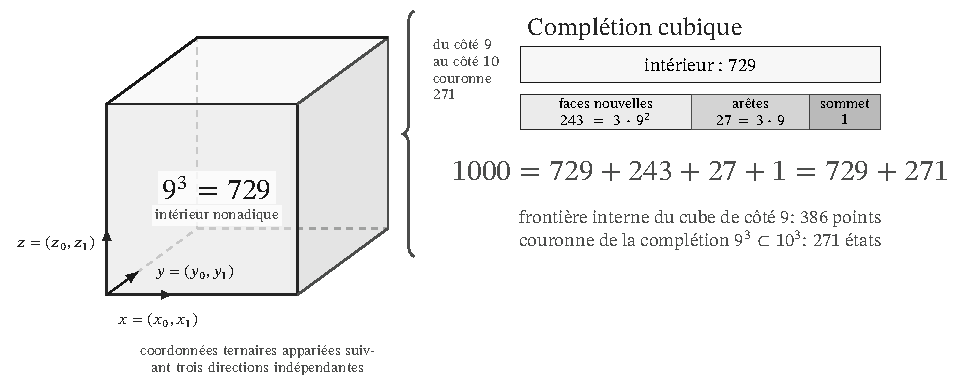
\includegraphics[width=\textwidth]{figures/cubo_emrh_original.pdf}
\caption{Représentation cubique de l'extension de neuf à dix classes par coordonnée. Les strates \(S_1,S_2,S_3\) placent les incidences ajoutées sur les faces, les arêtes et l'apex ; leurs cardinaux forment la couronne de \(271\) éléments. La frontière de \(386\) éléments appartient au cube initial. La perspective géométrique complète la partition de la figure ~\ref{vi:cubo:estratos-fig} ; les séparations graphiques ont une fonction schématique.}
\label{vi:cubo:completacion-3d}
\end{figure}


\subsubsection{Conservation de l'unité et compatibilité dimensionnelle}

La normalisation ne se limite pas à diviser une identité isolée. En dimension
\(d\), le produit \(\widehat E^d\) porte la mesure uniforme
\(\mu_d(\{x\})=10^{-d}\). La projection coordonnée
\(p_d:\widehat E^{d+1}\to\widehat E^d\) supprime la dernière coordonnée.

\begin{proposition}[Compatibilité projective des mesures normalisées]
Pour tout \(d\geq1\),
\[
 (p_d)_*\mu_{d+1}=\mu_d,
 \qquad \mu_d(\widehat E^d)=1.
\]
La masse de la strate comportant \(r\) coordonnées supplémentaires est
\(\binom dr9^{d-r}/10^d\), et la somme des masses de toutes les strates
vaut un.
\end{proposition}
\begin{proof}
Chaque point de \(\widehat E^d\) possède dix préimages. Leur masse totale est
\(10\,10^{-(d+1)}=10^{-d}\). L'égalité pour tout sous-ensemble
s'obtient en sommant sur ses points. La formule stratifiée provient
du même dénombrement que \eqref{vi:cubo:estratos} ; le binôme
\((9+1)^d\) donne la normalisation totale.
\end{proof}

En dimension trois, retirer l'apex laisse une masse \(999/1000\), et
le restituer ajoute \(1/1000\). Renormaliser avant la restitution
définirait une autre mesure : la distinction est pertinente sur le plan opératoire.
En particulier, conservation de la masse probabiliste, conservation des
registres de transport et dissipation thermodynamique sont des affirmations portant sur
des objets différents. La proposition démontre la première et fournit le
support compatible pour étudier la deuxième ; la troisième requiert une
réalisation dynamique et énergétique spécifiée.

La frontière géométrique interne demeure également distincte.
Sur le représentant cartésien \(\{1,\ldots,9\}^3\), retirer
\(\{2,\ldots,8\}^3\) laisse \(386\) points. Cette frontière appartient au
cube initial, tandis que \(\widehat C\setminus C\) appartient à son
extension. La complétion cubique, le développement positionnel en base mille et
la lecture d'incidence exceptionnelle partagent des données du support ;
leurs applications respectives déterminent l'information issue de ces données qu'utilise
chaque représentation.


\subsection{Sélection des régions par fibres orientées}

Pour \(w=(w_1,\ldots,w_6)\), définissons
\[
 r(w)=(w_3,w_1,w_2,w_5,w_6,w_4),\qquad
 s(w)=(w_4,w_5,w_6,w_1,w_2,w_3).
\]
Les identités \(r^3=s^2=I\), \(srs=r^{-1}\) réalisent
\(D_3\). Permuter de la même manière les six composantes de \(U\)
commute avec \(\Psi\). L’énumération précédente vérifie que les
orbites conservent les multiplicités de leurs fibres.

Soient \(f(w)\) le nombre d’émissions sur \(w\), \(m(w)\)
leur multiplicité totale et \(\nu(w)=(n_0,n_1,n_2)\) leur recensement
ternaire. La signature additive conserve la classe diagonale
\(d=[i+j]_9\) de l’origine et le sens \(ES\) ou \(NO\).
Nous écrivons \(\mathcal D(\mathcal O)\) pour l’ensemble de ces
classes sur une orbite.

\begin{proposition}[Régions distinguées du catalogue]
\label{vi:reg:seleccion}
Il existe une unique orbite de six mots avec cinq émissions par
mot et des multiplicités \(432+4\cdot144\). Parmi les orbites
de six mots qui satisfont
\[
 f(w)=1,\quad m(w)=144\quad(w\in\mathcal O),\qquad
 \mathcal D(\mathcal O)=\{0,3,6\},
\]
le recensement \((2,3,1)\) et le recensement \((2,2,2)\) sélectionnent,
chacun, une unique orbite. La marque \(d=6\) avec l’orientation
\(ES\) détermine les représentants
\[
 w^{\rm cl}=010211,\qquad w^{\rm pr}=201101,
 \qquad w^{\rm au}=121200.
\]
\end{proposition}
\begin{proof}
Le tableau complet des \(43\) orbites dans
\ref{vi:reg:tablas} permet d’appliquer les prédicats. L’orbite de
clôture est la seule ayant une fibre de taille cinq et de poids \(1008\) ;
ses cinq poids sont ceux indiqués. La condition diagonale et la
fibre simple de poids \(144\) laissent six orbites. Leurs recensements
sélectionnent respectivement une orbite avec \((2,3,1)\) et une avec
\((2,2,2)\). Appliquer les six permutations de \(D_3\) et
vérifier la classe diagonale et l’orientation dans
\eqref{vi:reg:firmas} fixe les trois représentants écrits.
L’unicité utilise toutes les conditions : si l’on omet l’ensemble des
diagonales, quatre orbites équilibrées de fibre simple
et de poids \(144\) apparaissent.
\end{proof}

Les désignations clôture, propagation et auto-échelle s’appliquent
d’abord à ces régions. La section suivante introduit leurs
caractères d’évaluation. En particulier, la signature multiplicative
\(555555\) distingue une émission transversale de clôture, tandis
que \((5,5)\) est une position du support électronique. Les deux
constructions sont reliées par des opérations ultérieures et non
par l’identité de leurs chiffres.

\subsubsection{Involution spéculaire des composantes régionales}
\label{mono-ampl:regiones}

Sur le bloc régional
\(B=(u^{\rm cl},u^{\rm pr},u^{\rm au})\in(\FF_3^6)^3\),
l’échange est
\[
 \mathfrak cB=(u^{\rm pr},u^{\rm cl},u^{\rm au}).
\]
Son carré est l’identité et il maintient la composante d’auto-échelle.
Si \(q=u^{\rm cl}+u^{\rm pr}+u^{\rm au}\),
\(a=u^{\rm cl}+u^{\rm pr}-u^{\rm au}\) et
\(d=u^{\rm cl}-u^{\rm pr}\), on récupère le bloc par
\[
 u^{\rm au}=2(q-a),\quad s=q-u^{\rm au},\quad
 u^{\rm cl}=2(s+d),\quad u^{\rm pr}=2(s-d).
\]
La démonstration utilise \(2^{-1}=2\) dans \(\FF_3\). L’échange
conserve \(q,a,s\) et change le signe de \(d\). Par conséquent,
l’agrégat symétrique et la différence orientée conservent ensemble
les deux composantes que l’agrégat isolé ne distingue pas.
Cette involution régionale et l’inversion d’une route cardinale
agissent sur des domaines distincts. La composante fixe peut
évoluer pendant le transport tout en étant fixe sous l’échange.

\subsection{Calendrier, monodromie et mémoire}

Le calendrier fini se compose de douze fenêtres nonadiques. Sa
suite de groupes est
\begin{equation}
 0\longrightarrow C_{12}\xrightarrow{[b]\mapsto[9b]}C_{108}
 \xrightarrow{[t]\mapsto[t]_9}C_9\longrightarrow0.
 \label{eq:extension108}
\end{equation}
Pour \(t=9b+r\), \(0\le r<9\), la composition contient
le quotient de transport
\[
 (b,r)+(b',r')=
 \left(b+b'+\left\lfloor\frac{r+r'}9\right\rfloor,
       [r+r']_9\right),
\]
en réduisant la première coordonnée modulo douze. La projection est
exacte car son noyau est constitué des multiples de neuf. Elle n’admet pas de
section homomorphe : celle-ci donnerait \(C_{108}\cong C_{12}\times C_9\),
mais les exposants respectifs sont \(108\) et \(36\).

La monodromie décrit l’action d’un tour de la base de phase
sur sa fibre. Dans la dynamique avec mémoire, l’holonomie nonadique
\(\Gamma_9\) conserve la phase et avance la profondeur. Sa
projection sur la phase et le compteur vérifie
\[
 (r,n)\longmapsto(r,n+1).
\]
Cette formule est une représentation réduite de l’action, non une
définition qui élimine le reste de l’état. Sur des histoires
bidirectionnelles, le compteur peut être étendu à \(\ZZ\) ; sur des
histoires commencées à profondeur zéro, le recul n’est
défini que là où le prédécesseur est conservé. Le calendrier peut
revenir au bout de \(108\) transitions et conserver une mémoire
distincte de l’initiale. Cette distinction sera essentielle lorsque la
particule sera construite comme persistance et non comme répétition d’une
coordonnée visible.

\subsection{Des registres aux opérateurs de prolongement}

Les opérateurs linéaires de représentation sont déterminés sur les
transitions du transport. Si \(x_j^\chi\) est un état régional
et \(\Pi_6\) sa représentation à six composantes, la dépendance est
\[
 b_j^\chi=\Pi_6(x_j^\chi),\qquad
 x_{j+1}^\chi=U_{9j+9}\cdots U_{9j+1}(x_j^\chi).
\]
Les matrices des origines \(X_a\) et des destinations \(Y_a\), en
vecteurs lignes de \(\FF_3^6\), sont
\[
\begin{array}{c|c|c|c}
X_0&Y_0&X_1&Y_1\\\hline
010211&012222&010211&002111\\
012222&010211&002111&110221\\
201101&121221&102011&012222\\
121221&102011&012222&102011\\
121200&112202&121020&010210\\
112202&121020&010210&010200
\end{array}
\]
On a \(\det X_0=1\), \(\det X_1=-1\) dans \(\FF_3\).
La solution unique de \(X_aL_a=Y_a\) est \(L_a=X_a^{-1}Y_a\).
La concaténation des blocs exprimés dans le calendrier
\((L_0,L_0,L_1,L_1)\) produit les longueurs
\(6,12,18,24,30\). La frontière de longueur \(36\) conserve
le terminal et la relation de prolongement. Ces matrices
représentent des transitions : l’inversion linéaire prouve leur unicité
pour le registre donné, tandis que la génération des états
appartient à la composition effective \(U_t\) du TPK.

\subsection{Portée de la construction régionale dans l’étude des masses}

Le recensement a séparé conditions initiales, émissions, régions et
opérateurs représentant leurs transitions. L’étape suivante
évalue les coordonnées régionales et compose le registre dodécaphasique.
Plus loin, l’atlas des particules sera construit sur le même
support mais utilisera une autre classification. Cette continuité préserve
une provenance commune sans transformer une fibre numérique en une
espèce par simple coïncidence de cardinaux ou d’étiquettes.

\clearpage% Reunión focal desde I/sections/aritmetica_historias.tex, leído íntegro.
% Procedencia: technical/PROCEDENCIA_ARITMETICA_HISTORIAS_VI.md.
% Se conservan hist:seccion e hist:doble-varianza para el núcleo común.
% No incluye la representación de Weyl ni la prolongación excepcional de I.
\section{Arithmétique des histoires, composition et raffinement}
\label{vi:hist:seccion-principal}

La persistance d’une particule et l’évaluation de son caractère nécessitent
de distinguer l’histoire transportée des coordonnées qui y sont lues.
Le noyau APP--TRIT--TPK fournit les états admissibles, leurs routes et
les opérations qui conservent leur provenance. Cette section précise trois
structures utilisées lors du passage de ces données à l’atlas : la compatibilité
entre profondeurs, la composition d’histoires avec mémoire et le
transport des observables en sens contraire au raffinement.
Les coefficients algébriques agissent sur des états et des routes déjà spécifiés ;
les relations prouvées ci-dessous conservent cet ordre.

\subsection{Sections compatibles et évaluation de leurs lecteurs}
\label{hist:seccion}

Soit \(X_n\) l’ensemble des états admissibles de profondeur \(n\)
produits par le noyau. Un état enregistre les positions d’APP, les
feuillets additif et multiplicatif, leurs résidus et quotients, le régime
tritique, l’orientation, la phase, la frontière, la route, la retenue et la
mémoire pertinente pour la survie. Ces données satisfont les
relations des opérations qui les ont produites ; elles ne sont pas considérées comme un
produit de coordonnées indépendantes.

Pour \(m\ge n\), la restriction
\(r_{m,n}:X_m\longrightarrow X_n\) conserve l’antécédent de profondeur
\(n\). Les restrictions satisfont
\begin{equation}
 r_{n,n}=\operatorname{id}_{X_n},\qquad
 r_{\ell,n}=r_{m,n}\circ r_{\ell,m}
 \quad(\ell\ge m\ge n).
 \label{vi:hist:restricciones}
\end{equation}
La nouvelle mémoire appartient au prolongement ; la restriction conserve celle
qui était déjà déterminée dans le préfixe.

\begin{definition}[Section numérique compatible]
Une section numérique HMT est une suite d’états de la même généalogie
\begin{equation}
 x=(x_n)_{n\ge0}\in X_\infty:=\varprojlim_n X_n,
 \qquad r_{m,n}(x_m)=x_n\quad(m\ge n).
 \label{vi:hist:limite-inverso}
\end{equation}
Un lecteur est une opération définie sur un domaine déterminé de ces
sections. Une observation finie appartient à un préfixe ; une valeur scalaire
est l’évaluation d’un lecteur. La section et la présentation de cette section
par un lecteur sont donc des objets de types distincts.
\end{definition}

La notation de limite projective réunit la compatibilité des états déjà
construits. L’existence d’un prolongement concret est établie
par les règles d’admissibilité de cette construction, non par la
seule écriture de \(X_\infty\).

Dans le domaine archimédien d’un lecteur, chaque préfixe détermine un
intervalle fermé non vide \(I_n(x)=[a_n(x),b_n(x)]\), avec
\begin{equation}
 I_{n+1}(x)\subseteq I_n(x),\qquad
 b_n(x)-a_n(x)\longrightarrow0.
 \label{vi:hist:cilindros}
\end{equation}
L’évaluation régionale par intervalles et la détermination de ses préfixes ont
été réunies dans la proposition~\ref{vi:dep:prefijos}.

\begin{proposition}[Valeur déterminée par des cylindres compatibles]
Pour toute section de ce domaine, il existe un unique nombre réel
\(\operatorname{ev}(x)\) tel que
\begin{equation}
 \{\operatorname{ev}(x)\}=\bigcap_{n\ge0}I_n(x).
 \label{vi:hist:evaluacion}
\end{equation}
\end{proposition}
\begin{proof}
L’emboîtement rend la suite \(a_n(x)\) croissante et
\(b_n(x)\) décroissante. Toutes deux restent bornées dans l’intervalle initial. Par
complétude de la droite, \(a=\sup_n a_n(x)\) et
\(b=\inf_n b_n(x)\) existent et satisfont \(a\le b\).
La largeur tendant vers zéro impose \(a=b\). Ce point appartient à chaque
intervalle et tout autre point de l’intersection aurait une distance à
celui-ci inférieure ou égale à toutes les largeurs ; il coïnciderait donc avec lui.
\end{proof}

Cette proposition détermine la valeur de chaque section du domaine indiqué.
Une couverture de toute \(\mathbb R\) nécessite de prouver que chaque valeur
appartient à l’image du lecteur ; la définition de la limite projective ne
fournit pas à elle seule cette preuve. De même, l’identification de deux
histoires à partir de leur valeur nécessite un résultat d’injectivité
pour le lecteur considéré. L’évaluation conserve la généalogie comme
antécédent et spécifie exactement quelle partie de celle-ci elle exprime.

\subsection{Algèbre sectorielle des routes et multiplicateurs de mémoire}
\label{vi:hist:algebra}

Fixons un secteur d’états et la catégorie \(\mathcal C\) de leurs
histoires admissibles. Nous écrivons \(vu=v\circ u\) : on parcourt d’abord
\(u\), puis \(v\). Les pas élémentaires sont des opérations de
sélection, de transport et de mise à jour du TPK. La catégorie conserve
leurs extrémités et les conditions permettant de concaténer deux routes.

La fibre tritique locale peut être représentée par
\[
 \mathbb R[J_x]/(J_x^2+\tau(x)1_x),
 \qquad \tau(x)\in\{+1,0,-1\}.
\]
La représentation conserve le régime et son orientation. Pour traiter
des coefficients plus riches, nous admettrons une algèbre réelle associative et
unitale \(A_x\) en chaque objet \(x\). Une transition entre régimes
doit préciser son application sur ces algèbres ; elle ne revient pas à les identifier.

La construction suivante s’applique aux secteurs possédant des transports
unitaux \(\rho_u:A_x\to A_y\), pour \(u:x\to y\), avec
\begin{equation}
 \rho_{\operatorname{id}_x}=\operatorname{id}_{A_x},\qquad
 \rho_v\circ\rho_u=\rho_{vu}.
 \label{vi:hist:accion}
\end{equation}
Pour chaque paire composable \(u:x\to y\), \(v:y\to z\), soit
\(\Omega(v,u)\in Z(A_z)^\times\) un multiplicateur central inversible.
Ses règles sont
\begin{equation}
 \Omega(\operatorname{id}_y,u)
 =\Omega(u,\operatorname{id}_x)=1_y
 \label{vi:hist:normalizacion}
\end{equation}
et, pour \(w:z\to t\),
\begin{equation}
 \rho_w\!\left(\Omega(v,u)\right)\Omega(w,vu)
 =\Omega(w,v)\Omega(wv,u).
 \label{vi:hist:cociclo}
\end{equation}
Ces conditions décrivent la structure de départ du secteur : chaque
application concrète doit fournir ses transports et ses multiplicateurs.
Une réalisation par bimodules conserve ses propres compositions et
n’est pas automatiquement remplacée par l’action stricte
\eqref{vi:hist:accion}.

Soit \(t(u)\) l’extrémité terminale de la flèche \(u\). Sur les sommes
à support fini
\[
 \mathcal H=\bigoplus_{u\in\operatorname{Mor}(\mathcal C)}A_{t(u)}T_u
\]
nous définissons par bilinéarité
\begin{equation}
 (aT_v)(bT_u)=
 a\rho_v(b)\Omega(v,u)T_{vu}
 \label{vi:hist:producto}
\end{equation}
lorsque \(u,v\) sont composables, et zéro sinon. La somme réunit
des histoires avec leurs coefficients ; le produit concatène les histoires et
conserve le multiplicateur de mémoire. Le support fini assure que chaque
produit est défini sans exiger de convergence supplémentaire.

\subsection{Associativité, identités locales et mémoire du calendrier}
\label{vi:hist:asociatividad}

\begin{proposition}[Composition associative du secteur]
Sous \eqref{vi:hist:accion}--\eqref{vi:hist:cociclo}, le produit
\eqref{vi:hist:producto} est associatif. S’il y a un nombre fini d’objets, son unité
est \(\sum_x1_xT_{\operatorname{id}_x}\). Pour un ensemble d’objets
arbitraire, les mêmes expressions sur des ensembles finis d’extrémités
donnent des identités locales pour toute collection finie d’histoires.
\end{proposition}
\begin{proof}
Soient \(u:x\to y\), \(v:y\to z\), \(w:z\to t\), avec des coefficients
\(a\in A_y\), \(b\in A_z\), \(c\in A_t\). Les deux associations
produisent comme coefficients de \(T_{wvu}\)
\begin{align*}
 ((cT_w)(bT_v))(aT_u):\quad&
 c\rho_w(b)\Omega(w,v)\rho_{wv}(a)\Omega(wv,u),\\
 (cT_w)((bT_v)(aT_u)):\quad&
 c\rho_w(b)\rho_w\rho_v(a)
 \rho_w(\Omega(v,u))\Omega(w,vu).
\end{align*}
L’action stricte identifie \(\rho_w\rho_v(a)\) à
\(\rho_{wv}(a)\). La centralité permet de déplacer
\(\Omega(w,v)\) à droite de ce facteur, et l’identité de cocycle
rend égaux les facteurs restants. Les coefficients généraux
\(a,b,c\), qui peuvent ne pas commuter, ne sont pas permutés. Si les trois flèches ne forment pas une
chaîne composable, les deux associations sont nulles du fait de leurs extrémités.
La bilinéarité étend l’égalité aux sommes finies. Enfin,
\eqref{vi:hist:normalizacion} et l’unitalité de chaque \(\rho_u\)
vérifient l’unité. Pour une collection finie, il suffit de sommer les identités
de toutes ses extrémités initiales et terminales, ce qui démontre la dernière
affirmation.
\end{proof}

Le calendrier nonadique fournit une réalisation effective de ces
conditions. Prenons la catégorie à un objet avec des flèches
\(C_9=\mathbb Z/9\mathbb Z\), des coefficients
\(A=\mathbb R[z,z^{-1}]\) et l’action identité. Pour des représentants
\(0\le a,b<9\), nous définissons
\begin{equation}
 c_0(a,b)=\left\lfloor\frac{a+b}{9}\right\rfloor,
 \qquad\Omega(b,a)=z^{c_0(a,b)}.
 \label{vi:hist:carry-calendario}
\end{equation}
La variable formelle \(z\) conserve le nombre de tours. La normalisation
découle de \(c_0(0,a)=c_0(a,0)=0\). Si \([a+b]_9\) désigne le
représentant réduit, la division euclidienne donne
\[
 c_0(a,b)+c_0([a+b]_9,c)
 =\left\lfloor\frac{a+b+c}{9}\right\rfloor
 =c_0(b,c)+c_0(a,[b+c]_9).
\]
Cette égalité prouve le cocycle \eqref{vi:hist:cociclo} pour les
multiplicateurs, et donc l’associativité du calendrier avec mémoire.

Si \(T=T_{[1]_9}\), les règles du produit donnent
\(T^j=T_{[j]_9}\) pour \(0\le j<9\) et \(T^9=zT_{[0]_9}\).
En imposant ensuite \(z^{12}=1\), on obtient \(T^{108}=1\).
Les expressions \(z^kT_{[j]_9}\), \(0\le k<12\), \(0\le j<9\),
forment les \(108\) positions du calendrier résultant. On récupère ainsi
le groupe cyclique \(C_{108}\) et sa projection sur \(C_9\) ; conserver
\(z\) sans cette relation distingue les tours successifs. C’est une
réalisation de la mémoire de calendrier : les autres coordonnées des
histoires TPK restent dans leur domaine propre.

\subsection{Double variance du raffinement et conservation de l’unité}
\label{hist:doble-varianza}

La restriction des états induit un prolongement des observables en sens
contraire. Pour les algèbres de fonctions munies du produit ponctuel
\(D_n=\operatorname{Fun}(X_n,\mathbb R)\), la précomposition définit
\begin{equation}
 r_{m,n}^*:D_n\longrightarrow D_m,
 \qquad r_{m,n}^*f=f\circ r_{m,n}.
 \label{vi:hist:precomposicion}
\end{equation}
L’ordre contravariant
\(r_{\ell,n}^*=r_{\ell,m}^*\circ r_{m,n}^*\) est conservé. Ces applications
sont des homomorphismes unitaux. Si \(r_{m,n}\) est surjective, alors
\(r_{m,n}^*\) est également injective : une différence entre deux fonctions peut
être évaluée en un antécédent d’un point où elles diffèrent.

\begin{lemma}[Indicatrices, unité et évaluation compatible]
Pour \(x\in X_n\), soit \(e_x\) sa fonction indicatrice. Alors
\begin{equation}
 r_{m,n}^*e_x=\mathbf1_{r_{m,n}^{-1}(x)},\qquad
 r_{m,n}^*1_n=1_m.
 \label{vi:hist:unidad}
\end{equation}
Lorsque la fibre \(r_{m,n}^{-1}(x)\) est finie, la première égalité est
la somme finie
\[
 r_{m,n}^*e_x=\sum_{y:\,r_{m,n}(y)=x}e_y.
\]
Pour toute section \(x=(x_n)\in X_\infty\), la règle
\([f]\mapsto f(x_n)\), avec \(f\in D_n\), définit un homomorphisme
unital
\begin{equation}
 \operatorname{Ev}_x:D_{\mathrm{cyl}}\longrightarrow\mathbb R,
 \qquad
 D_{\mathrm{cyl}}=\varinjlim_n(D_n,r_{n+1,n}^*).
 \label{vi:hist:evaluacion-observables}
\end{equation}
\end{lemma}
\begin{proof}
Pour \(y\in X_m\), on a
\((r_{m,n}^*e_x)(y)=1\) exactement lorsque \(r_{m,n}(y)=x\).
C’est la première égalité de \eqref{vi:hist:unidad}. Si la fibre est
finie, ses indicatrices ponctuelles sont orthogonales et leur somme est son indicatrice.
La seconde égalité s’obtient à partir de \(1_n(r_{m,n}(y))=1\), sans aucune
hypothèse sur le cardinal de la fibre.

Pour toute \(f\in D_n\), la naturalité de l’évaluation est
\[
 (r_{m,n}^*f)(y)=f(r_{m,n}(y)).
\]
Dans une section compatible, \(r_{m,n}(x_m)=x_n\), donc
\((r_{m,n}^*f)(x_m)=f(x_n)\). Par conséquent, deux représentants qui
s’identifient à une profondeur commune ont la même évaluation.
L’évaluation ponctuelle préserve somme, produit et unité, ce qui conclut
la preuve de \eqref{vi:hist:evaluacion-observables}.
\end{proof}

Pour les fibres infinies, la formulation au moyen de
\(\mathbf1_{r_{m,n}^{-1}(x)}\) reste valide ; il n’est pas nécessaire d’interpréter une somme
infinie comme une somme algébrique finie. La limite inductive réunit les
observables de profondeur finie avec les identifications induites par
les restrictions. Le prolongement des opérateurs de route exige, en outre,
les carrés de compatibilité de leurs transports avec ces restrictions.

L’unité conservée est la fonction constante égale à un sur le domaine des
possibilités. Une section individuelle sélectionne une histoire compatible
de ce domaine. Le raffinement peut augmenter la profondeur et distinguer
davantage de prolongements tout en préservant l’unité et l’évaluation de chaque
antécédent. Cette conservation unitale fournit le contenu algébrique
précis utilisé ici ; une mesure de probabilité, lorsqu’elle intervient dans
un autre lecteur, nécessite en outre sa normalisation et ses propres règles.

\clearpage% BEGIN NUCLEO_ADITIVO_20260921_SELECCION
\clearpage
% Ampliación demostrativa DF003--DF007. No modifica la fuente integral.
% Propietario común de los archivos Lean citados en estos comentarios:
% output/PAQUETE_ARTICULO_I_INTEGRACION_ESTADO_CAMPOS_20260919/.
% Residencia causal de la primera sección: después de los lectores regionales
% coinductivos y antes de emplear sus registros como entrada de la selección K.
% Residencia causal de la segunda sección: después de la construcción marcada
% Paley--Witt--Golay--Leech y antes de la reconstrucción de la estructura VOA.
% Los dos cortes expositivos conservan el mismo origen APP--TRIT--TPK.

\section[Génération régionale et raffinement]{Compatibilité intégrale de la génération régionale, du raffinement cylindrique et de l'incidence}
\label{act21:sec:df-lectores-cilindros}

La prolongation régionale produit des suites ordonnées de blocs, ainsi que
leurs profondeurs de lecture. La projection archimédienne et l'incidence
ternaire se calculent sur ces mêmes suites. Le lien entre ces deux
réalisations peut s'exprimer entièrement par des opérations entières :
sélection par intervalles rationnels, division euclidienne, élévation de six
trits, lecture de retenue et transformation de Witt. Cette formulation permet
de suivre chaque coefficient depuis son bloc générateur jusqu'à son emploi ultérieur.

La construction utilise les trois lecteurs régionaux déjà obtenus de l'état APP--TRIT--TPK. Nous les désignerons par les indices \(c\in\{\mathrm P,\mathrm E,\mathrm F\}\), correspondant respectivement aux régions de clôture, de propagation et d'auto-échelle. Leur réalisation réelle s'écrira \(v_c\). Les identifications ultérieures \(v_{\mathrm P}=\pi_{\mathrm{HMT}}\), \(v_{\mathrm E}=e_{\mathrm{HMT}}\) et \(v_{\mathrm F}=\varphi_{\mathrm{HMT}}\) conservent cet ordre causal. L'opération qui émet un bloc inspecte les intervalles rationnels du lecteur régional ; la valeur réelle intervient dans la démonstration de correction de cette opération.

\subsection{Émission positionnelle par séparation rationnelle de cellules}
\label{act21:subsec:df-emision-racional}

% Fuente: lean/biblioteca/RegionalPublicationComposition.lean,
% produced_brackets, eventual_publication, joint_eventual_publication,
% search_terminates, stopped_cell_correct, publications_compatible.

Pour chaque région, on dispose de deux suites rationnelles
\(\ell_c(j),u_c(j)\), construites par son lecteur, qui satisfont
\[
 \ell_c(j)\leq v_c\leq u_c(j).
\]
La propriété de séparation des cellules démontrée pour ces lecteurs affirme
que, pour chaque entier \(s>0\), il existe \(J\) tel que, pour tout \(j\geq J\),
\begin{equation}
 \lfloor s\ell_c(j)\rfloor
 =\lceil su_c(j)\rceil-1
 =\lfloor sv_c\rfloor.
 \label{act21:eq:df-separacion-celdas}
\end{equation}
L'évitement des frontières rationnelles par les valeurs régionales est l'hypothèse des théorèmes précédents qui garantit cette séparation. Ici, on emploie sa conclusion opérationnelle, avec les lecteurs et les intervalles qui la produisent.

\begin{definition}[Indice de séparation et préfixe émis]
Pour \(s>0\), soit
\[
 j_c(s)=\min\{j\in\mathbb N:
 \lfloor s\ell_c(j)\rfloor=\lceil su_c(j)\rceil-1\}.
\]
Pour une base entière \(b\geq2\) et une profondeur \(n\geq0\), on définit
\begin{equation}
 P_c(b,n)=\lfloor b^n\ell_c(j_c(b^n))\rfloor.
 \label{act21:eq:df-publicacion-prefijo}
\end{equation}
Le préfixe contient la partie entière et les premières \(n\) positions en base \(b\) ; par conséquent, \(P_c(b,0)\) est la partie entière régionale.
\end{definition}

\begin{theorem}[Terminaison et correction de l'émission]
\label{act21:thm:df-emision-correcta}
L'indice \(j_c(s)\) existe pour tout \(s>0\). Les préfixes émis satisfont
\begin{equation}
 P_c(b,n)=\lfloor b^n v_c\rfloor,
 \qquad
 P_c(b,n)\leq b^n v_c<P_c(b,n)+1.
 \label{act21:eq:df-prefijo-correcto}
\end{equation}
Pour chaque échelle \(s\) il est possible en outre de choisir un unique indice de suffisance \(J(s)\) valide simultanément pour les trois régions.
\end{theorem}

\begin{proof}
L'égalité à partir d'un certain rang de \eqref{act21:eq:df-separacion-celdas} rend non vide
l'ensemble qui définit \(j_c(s)\). Son minimum existe par le bon ordre de
\(\mathbb N\). À tout indice où l'égalité se produit, la borne
inférieure rationnelle fournit
\(\lfloor s\ell_c(j)\rfloor\leq\lfloor sv_c\rfloor\).
La borne supérieure, jointe à l'évitement d'une frontière de cellule, donne
\(\lfloor sv_c\rfloor\leq\lceil su_c(j)\rceil-1\).
Les deux extrémités entières coïncidant, l'entier intermédiaire coïncide avec
elles. Cela démontre \eqref{act21:eq:df-prefijo-correcto}. Pour l'affirmation
conjointe, il suffit de prendre le maximum des trois indices de suffisance obtenus
pour la même échelle. L'indice conjoint contrôle simultanément les trois
émissions, tandis que chaque région conserve ses propres intervalles.
\end{proof}

\begin{proposition}[Compatibilité exacte des préfixes]
\label{act21:prop:df-prefijos-compatibles}
Pour \(n,m\geq0\),
\begin{equation}
 \left\lfloor\frac{P_c(b,n+m)}{b^m}\right\rfloor=P_c(b,n).
 \label{act21:eq:df-truncamiento}
\end{equation}
En particulier, le bloc suivant
\(d_c(b,n)=P_c(b,n+1)\bmod b\) satisfait
\begin{equation}
 P_c(b,n+1)=bP_c(b,n)+d_c(b,n),\qquad 0\leq d_c(b,n)<b.
 \label{act21:eq:df-paso-posicional}
\end{equation}
\end{proposition}

\begin{proof}
Écrivons \(b^n v_c=N+\theta\), avec
\(N=P_c(b,n)\) et \(0\leq\theta<1\). Alors
\(P_c(b,n+m)=b^mN+\lfloor b^m\theta\rfloor\), et le second terme
appartient à \(\{0,\ldots,b^m-1\}\). La division euclidienne par \(b^m\)
récupère \(N\). La spécialisation \(m=1\) produit
\eqref{act21:eq:df-paso-posicional} et sa borne résiduelle.
\end{proof}

\subsection{Blocs régionaux de six trits à profondeur arbitraire}
\label{act21:subsec:df-bloques-arbitrarios}

% Fuente: deltas/integracion/JointRegionalFrontier.lean,
% publish_base729_eq_base3, generated_block_from_longer_prefix,
% generated_block_eq_finite, generated_signature_eq_finite.

L'égalité entière \(729=3^6\) détermine le regroupement de six positions ternaires en un bloc. Pour \(t\geq0\), nous définissons
\begin{equation}
 u_c(t)=P_c(729,t+1)\bmod729,
 \qquad
 B_{c,j}(t)=
 \left\lfloor\frac{u_c(t)}{3^{5-j}}\right\rfloor\bmod3,
 \quad 0\leq j<6.
 \label{act21:eq:df-bloque-y-banda}
\end{equation}
Ainsi, \(B_c(t)\) est un mot ordonné de six trits et
\begin{equation}
 u_c(t)=\sum_{j=0}^{5}B_{c,j}(t)3^{5-j}.
 \label{act21:eq:df-elevacion-banda}
\end{equation}
Le mot et son élévation entière sont deux représentations mutuellement récupérables du même bloc émis.

\begin{theorem}[Stabilité d'extraction à toute profondeur]
\label{act21:thm:df-bloque-estable}
On vérifie, pour tout \(n\),
\[
 P_c(729,n)=P_c(3,6n).
\]
Si \(t<n\), alors
\begin{equation}
 u_c(t)=
 \left\lfloor\frac{P_c(729,n)}{729^{n-t-1}}\right\rfloor\bmod729.
 \label{act21:eq:df-bloque-prefijo-largo}
\end{equation}
En conséquence, toute extension du préfixe préserve tous les
blocs précédemment émis et toutes les signatures calculées dessus.
\end{theorem}

\begin{proof}
La première égalité résulte de ce que les deux préfixes se séparent à la même
échelle, \(729^n=3^{6n}\), et du
théorème~\ref{act21:thm:df-emision-correcta}. Pour la seconde, nous appliquons
\eqref{act21:eq:df-truncamiento} aux profondeurs \(n\) et \(t+1\), puis
nous prenons le résidu modulo \(729\). L'extraction ternaire de
\eqref{act21:eq:df-bloque-y-banda} est déterministe. Toute fonction explicite
de ces dix-huit coordonnées conserve, par conséquent, le même résultat en
étendant le préfixe.
\end{proof}

La construction est quantifiée sur \(t\in\mathbb N\). Une table qui
matérialise cent blocs constitue une évaluation finie de cette
construction ; la formule \eqref{act21:eq:df-bloque-prefijo-largo} détermine
exactement sa compatibilité avec toute extension ultérieure.

\begin{example}[Premier bloc conjoint]
L'évaluation des lecteurs régionaux sélectionnés donne les mots
\[
 B_{\mathrm P}(0)=010211,\qquad
 B_{\mathrm E}(0)=201101,\qquad
 B_{\mathrm F}(0)=121200.
\]
Leur élévation par \eqref{act21:eq:df-elevacion-banda} produit
\[
 u_{\mathrm P}(0)=103,\qquad
 u_{\mathrm E}(0)=523,\qquad
 u_{\mathrm F}(0)=450.
\]
Par exemple,
\(201101_3=2\cdot243+27+9+1=523\).
Les six positions, y compris les zéros initiaux, sont conservées dans la
représentation en bande. Le zéro initial de \(010211\) possède une position
définie, bien que l'écriture décimale de \(103\) en soit dépourvue.
\end{example}

\subsection{Registres de transition et reconstruction des élévations linéaires}
\label{act21:subsec:df-registros-transicion}

% Fuentes: deltas/integracion/RegionalTransitionRecords.lean y
% GeneratedTransitionRecords.lean; lean/biblioteca/TPKLifts.lean.
% Los enlaces reconstruidos son R(0)->R(1) y R(2)->R(3).

Sur \(\mathbb F_3\), nous réunissons deux émissions consécutives de chaque région dans la matrice
\begin{equation}
 R(t)=
 \begin{pmatrix}
 B_{\mathrm P}(t)\\ B_{\mathrm P}(t+1)\\
 B_{\mathrm E}(t)\\ B_{\mathrm E}(t+1)\\
 B_{\mathrm F}(t)\\ B_{\mathrm F}(t+1)
 \end{pmatrix}.
 \label{act21:eq:df-registro-matricial}
\end{equation}
Cette définition fixe à la fois l'ordre régional et l'ordre temporel. Les
quatre premiers registres sont
\[
 X_0=R(0),\quad Y_0=R(1),\quad X_1=R(2),\quad Y_1=R(3).
\]
Ses valeurs, obtenues par extraction des préfixes régionaux, sont
\begin{align*}
 X_0&=\begin{pmatrix}
0&1&0&2&1&1\\0&1&2&2&2&2\\2&0&1&1&0&1\\
1&2&1&2&2&1\\1&2&1&2&0&0\\1&1&2&2&0&2
\end{pmatrix},&
 Y_0&=\begin{pmatrix}
0&1&2&2&2&2\\0&1&0&2&1&1\\1&2&1&2&2&1\\
1&0&2&0&1&1\\1&1&2&2&0&2\\1&2&1&0&2&0
\end{pmatrix},\\[1ex]
 X_1&=\begin{pmatrix}
0&1&0&2&1&1\\0&0&2&1&1&1\\1&0&2&0&1&1\\
0&1&2&2&2&2\\1&2&1&0&2&0\\0&1&0&2&1&0
\end{pmatrix},&
 Y_1&=\begin{pmatrix}
0&0&2&1&1&1\\1&1&0&2&2&1\\0&1&2&2&2&2\\
1&0&2&0&1&1\\0&1&0&2&1&0\\0&1&0&2&0&0
\end{pmatrix}.
\end{align*}

\begin{theorem}[Reconstruction unique des deux liens initiaux]
\label{act21:thm:df-elevaciones-reconstruidas}
Les équations \(X_0L_0=Y_0\) et \(X_1L_1=Y_1\) ont, chacune, une
unique solution dans \(M_6(\mathbb F_3)\). Ces solutions sont
\begin{align*}
 L_0&=\begin{pmatrix}
2&2&2&1&2&1\\2&1&2&2&1&1\\1&0&0&1&0&2\\
0&0&1&1&1&0\\2&2&2&0&2&1\\2&1&2&1&0&0
\end{pmatrix},&
 L_1&=\begin{pmatrix}
2&1&2&0&2&2\\1&2&1&1&2&0\\1&2&1&1&1&2\\
0&1&0&0&2&1\\2&0&2&1&0&1\\0&2&2&2&1&1
\end{pmatrix}.
\end{align*}
Les deux matrices sont inversibles.
\end{theorem}

\begin{proof}
Les matrices
\begin{align*}
 A_0&=\begin{pmatrix}
1&1&2&0&1&2\\0&0&1&0&0&1\\2&1&2&1&0&1\\
0&2&0&1&0&2\\2&1&1&0&2&2\\2&1&1&1&1&2
\end{pmatrix},&
 A_1&=\begin{pmatrix}
1&0&1&2&0&0\\0&0&1&1&2&2\\0&1&2&0&1&1\\
1&1&0&2&0&0\\1&1&2&1&1&2\\1&0&0&0&0&2
\end{pmatrix}
\end{align*}
satisfont \(A_iX_i=X_iA_i=I\), par multiplication dans \(\mathbb F_3\).
Par conséquent, les solutions sont imposées par \(L_i=A_iY_i\) ; la
multiplication produit les deux matrices montrées. Leurs inverses sont
\begin{align*}
 L_0^{-1}&=\begin{pmatrix}
1&2&0&2&0&2\\2&0&2&2&0&0\\2&1&2&0&2&0\\
1&0&0&0&2&0\\0&2&1&1&2&0\\2&2&2&2&2&2
\end{pmatrix},&
 L_1^{-1}&=\begin{pmatrix}
2&0&2&1&2&1\\2&1&0&0&2&0\\2&0&2&2&0&2\\
2&0&0&1&1&0\\1&1&1&1&1&0\\2&0&1&2&2&0
\end{pmatrix}.
\end{align*}
La vérification bilatérale \(L_iL_i^{-1}=L_i^{-1}L_i=I\) démontre la
récupération exacte de chaque mot transformé. Tous les produits
utilisent des résidus \(0,1,2\), avec leur interprétation en \(\mathbb F_3\).
\end{proof}

La lecture causale de ce résultat est précise : les émissions régionales produisent \(R(t)\) ; les registres \(R(0),\ldots,R(3)\) déterminent les deux élévations précédentes ; leurs inverses récupèrent les mots transformés.  
La continuité pour tout \(t\) appartient aux lecteurs coinductifs et au théorème ~\ref{act21:thm:df-bloque-estable}. La reconstruction matricielle démontrée ici a pour domaine les deux liens spécifiés dans son énoncé.

\subsection{Raffinement simultané dans les bases ternaire et décimale}
\label{act21:subsec:df-cilindros-mixtos}

% Fuente: deltas/integracion/RegionalCylinderTransition.lean.

Une émission ternaire de six trits et une émission décimale de trois chiffres
constituent deux lectures de bases différentes. Pour conserver leur relation, on
enregistre l'état
\[
 s=(n,k,N,D),
\]
où \(N\) est un préfixe de profondeur \(n\) en base \(729\), et \(D\) est
un préfixe de profondeur \(k\) en base \(1000\). Leurs cylindres
archimédiens sont
\begin{equation}
 I_{729}(s)=\left[\frac{N}{729^n},\frac{N+1}{729^n}\right),\qquad
 I_{1000}(s)=\left[\frac{D}{1000^k},\frac{D+1}{1000^k}\right).
 \label{act21:eq:df-cilindros}
\end{equation}
L'extrémité supérieure semi-ouverte attribue chaque valeur à une unique cellule d'une base et d'une profondeur données.

\begin{definition}[Défauts entiers de compatibilité]
On définit
\begin{align}
 A(s)&=N1000^k-D729^n,\label{act21:eq:df-defecto-inferior}\\
 B(s)&=(N+1)1000^k-D729^n=A(s)+1000^k.
 \label{act21:eq:df-defecto-superior}
\end{align}
L'état est compatible lorsque
\begin{equation}
 A(s)<729^n,\qquad B(s)>0.
 \label{act21:eq:df-compatibilidad}
\end{equation}
\end{definition}

\begin{lemma}[Critère entier d'intersection]
Les cylindres de \eqref{act21:eq:df-cilindros} ont une intersection non vide si et
seulement si \eqref{act21:eq:df-compatibilidad} est vérifiée.
\end{lemma}

\begin{proof}
Deux intervalles semi-ouverts \([a,b)\) et \([c,d)\), avec \(a<b\) et
\(c<d\), se coupent exactement lorsque \(a<d\) et \(c<b\). En appliquant cette
condition à \eqref{act21:eq:df-cilindros} et en multipliant par les dénominateurs
positifs, nous obtenons
\(N1000^k<(D+1)729^n\) et
\(D729^n<(N+1)1000^k\). Ce sont les deux inégalités de
\eqref{act21:eq:df-compatibilidad}.
\end{proof}

\begin{definition}[Mise à jour des profondeurs et des préfixes]
Pour \(0\leq u<729\) et \(0\leq d<1000\), nous définissons
\begin{align*}
 T_u(n,k,N,D)&=(n+1,k,729N+u,D),\\
 T_{u,d}(n,k,N,D)&=(n+1,k+1,729N+u,1000D+d).
\end{align*}
La première opération raffine uniquement le cylindre ternaire. La seconde  
raffine les deux lectures et conserve les deux profondeurs dans l'état.
\end{definition}

\begin{proposition}[Récurrences exactes de frontière]
\label{act21:prop:df-rec-frontera}
Les mises à jour précédentes satisfont
\begin{align}
 A(T_u s)&=729A(s)+u1000^k,\label{act21:eq:df-rec-ternaria}\\
 A(T_{u,d}s)&=729000A(s)+u1000^{k+1}-d729^{n+1}.
 \label{act21:eq:df-rec-conjunta}
\end{align}
\end{proposition}

\begin{proof}
Pour la première identité,
\[
 (729N+u)1000^k-D729^{n+1}
 =729(N1000^k-D729^n)+u1000^k.
\]
Pour la seconde,
\begin{align*}
 &(729N+u)1000^{k+1}-(1000D+d)729^{n+1}\\
 &\qquad=729000(N1000^k-D729^n)
      +u1000^{k+1}-d729^{n+1}.
\end{align*}
Les deux sont des identités entières antérieures à toute approximation réelle.
\end{proof}

\begin{theorem}[Raffinement des cylindres régionaux générés]
\label{act21:thm:df-refinamiento-generado}
Soit
\[
 s_c(n,k)=(n,k,P_c(729,n),P_c(1000,k)).
\]
Alors \(s_c(n,k)\) est compatible quels que soient \(n,k\). De plus,
\begin{align*}
 T_{u_c(n)}s_c(n,k)&=s_c(n+1,k),\\
 T_{u_c(n),d_c(1000,k)}s_c(n,k)&=s_c(n+1,k+1).
\end{align*}
La division euclidienne des préfixes raffinés récupère exactement les
préfixes précédents. Pour tout \(a,b\geq0\),
\[
 \frac{P_c(729,n+a)-P_c(729,n+a)\bmod729^a}{729^a}
 =P_c(729,n),
\]
et l'identité analogue est vérifiée en base \(1000\).
\end{theorem}

\begin{proof}
Le théorème~\ref{act21:thm:df-emision-correcta} place \(v_c\) simultanément dans
les deux intervalles \eqref{act21:eq:df-cilindros} ; le critère d'intersection donne
la compatibilité. Les identités de mise à jour sont
\eqref{act21:eq:df-paso-posicional} dans chaque base. La récupération s'obtient à partir de
\eqref{act21:eq:df-truncamiento}. Par conséquent, la récurrence du défaut et la
récupération du préfixe sont des conséquences d'une même mise à jour.
\end{proof}

\begin{example}[Premier couple de cylindres régionaux]
Pour \(n=k=1\), l'évaluation des trois régions donne
\[
\begin{array}{c|rr|rr}
 c&N&D&A&B\\\hline
 \mathrm P&2290&3141&211&1211\\
 \mathrm E&1981&2718&-422&578\\
 \mathrm F&1179&1618&-522&478
\end{array}
\]
Dans les trois lignes \(A<729\) et \(B>0\). La première colonne de préfixes
se décompose comme \(2290=3\cdot729+103\),
\(1981=2\cdot729+523\) et \(1179=729+450\) : réapparaissent exactement les
blocs de six trits déjà émis. Les signes différents de \(A\) expriment
la position relative des deux extrémités inférieures, sans altérer la
appartenance commune de la valeur régionale.
\end{example}

\subsection{Sélection du bloc suivant par le lecteur régional}

La compatibilité de deux intervalles exprime une relation entre lectures. La détermination du bloc suivant utilise en outre l'intervalle rationnel produit par la région. Cette opération peut se formuler sans éliminer l'histoire de profondeur.

\begin{definition}[Admissibilité de la prolongation régionale]
\(c,n\) étant fixés, soient \(s=729^{n+1}\) et \(j=j_c(s)\). Un résidu
\(u\in\{0,\ldots,728\}\) est admissible lorsque
\begin{equation}
 \lfloor s\ell_c(j)\rfloor
 \leq729P_c(729,n)+u
 \leq\lceil su_c(j)\rceil-1.
 \label{act21:eq:df-admisibilidad}
\end{equation}
\end{definition}

\begin{theorem}[Unicité de la prolongation compatible avec le lecteur]
\label{act21:thm:df-prolongacion-unica}
La condition \eqref{act21:eq:df-admisibilidad} est équivalente à \(u=u_c(n)\).
Par conséquent, il existe exactement une prolongation admissible de chaque région
à chaque profondeur.
\end{theorem}

\begin{proof}
À l'indice de séparation, les deux extrémités entières de
\eqref{act21:eq:df-admisibilidad} coïncident avec \(P_c(729,n+1)\).
La condition est ainsi équivalente à
\(729P_c(729,n)+u=P_c(729,n+1)\).
Par \eqref{act21:eq:df-paso-posicional}, le côté droit est
\(729P_c(729,n)+u_c(n)\). L'annulation du terme commun donne l'égalité des résidus. Réciproquement, cette égalité satisfait la condition.
\end{proof}

La dépendance effective de cette sélection reste complètement déterminée :
région sélectionnée, lecteur rationnel, profondeur, indice de séparation,
préfixe antérieur et résidu suivant. Le défaut \(A\) résume une relation
de frontière ; l'état \((n,k,N,D)\) et les intervalles régionaux conservent
les données employées par la mise à jour.

\subsection{Signature ternaire, retenue, incidence de Witt et horloge de lecture}
\label{act21:subsec:df-firma-conjunta}

% Fuentes: lean/regional/N69RegionalSignature.lean,
% deltas/integracion/JointRegionalFrontier.lean y JointCylinderSignature.lean.

Une profondeur \(t\) étant fixée, écrivons \(B_{c,j}=B_{c,j}(t)\). Pour chaque colonne \(j\), on calcule les entiers et les résidus suivants :
\begin{align}
 S_j&=B_{\mathrm P,j}+B_{\mathrm E,j}+B_{\mathrm F,j},
 &q_j&=S_j\bmod3,
 &c_j&=\left\lfloor S_j/3\right\rfloor,
 \label{act21:eq:df-firma-qc}\\
 a_j&=(B_{\mathrm P,j}+B_{\mathrm E,j}-B_{\mathrm F,j})\bmod3,
 &w_j&=\sum_c\mathbf1_{B_{c,j}\ne0},
 &\bar w_j&=w_j\bmod3.
 \label{act21:eq:df-firma-axial}
\end{align}
Le résidu de l'expression axiale est pris dans les entiers. Une implémentation
avec des naturels le calcule comme
\((B_{\mathrm P,j}+B_{\mathrm E,j}+3-B_{\mathrm F,j})\bmod3\), qui le conserve
exactement.

La matrice d'incidence ternaire utilisée par le lecteur est
\begin{equation}
 W=\begin{pmatrix}
0&1&1&1&1&1\\
1&0&1&1&2&2\\
1&1&0&2&1&2\\
1&1&2&0&2&1\\
1&2&1&2&0&1\\
1&2&2&1&1&0
\end{pmatrix}.
\label{act21:eq:df-matriz-witt}
\end{equation}
Pour chaque région, deux charges résiduelles sont conservées :
\begin{equation}
 v_c^{\mathrm{res}}=\sum_j B_{c,j}\bmod3,
 \qquad
 v_c^{\mathrm W}=\sum_j(B_cW)_j\bmod3.
 \label{act21:eq:df-cargas-residuales}
\end{equation}
La signature complète du lecteur est
\(\mathcal S(B)=(q,a,c,w,\bar w,v^{\mathrm{res}},v^{\mathrm W})\).
Sa structure conserve séparément le reste de colonne, la retenue, le
contraste axial, le poids de support et les deux lectures de charge.

\begin{theorem}[Récupération exacte et bornes de la signature]
\label{act21:thm:df-recuperacion-firma}
Pour chaque colonne et chaque région, on a
\begin{align}
 S_j&=q_j+3c_j,&0\leq q_j,a_j&<3,&0\leq c_j&\leq2,
 \label{act21:eq:df-recuperacion-total}\\
 B_{\mathrm F,j}&=2(q_j+3-a_j)\bmod3,&0\leq w_j&\leq3,
 &0\leq\bar w_j&<3.
 \label{act21:eq:df-recuperacion-eje}
\end{align}
De plus,
\begin{equation}
 v_c^{\mathrm W}
 =\left(\sum_j\bigl((B_cW)_j\bmod3\bigr)\right)\bmod3.
 \label{act21:eq:df-witt-reduccion}
\end{equation}
Les récupérations énoncées déterminent le total de chaque colonne et sa
coordonnée d'auto-échelle ; le registre régional conserve en outre
les trois bandes ordonnées.
\end{theorem}

\begin{proof}
L'identité \eqref{act21:eq:df-recuperacion-total} est la division euclidienne de
\(S_j\) par \(3\). Chaque terme de \(S_j\) est entre \(0\) et \(2\),
de telle sorte que \(0\leq S_j\leq6\) et \(c_j\leq2\). En \(\mathbb F_3\),
la soustraction des deux congruences qui définissent \(q_j\) et \(a_j\) donne
\(q_j-a_j=2B_{\mathrm F,j}\). Comme l'inverse de \(2\) est \(2\), on
obtient \eqref{act21:eq:df-recuperacion-eje} ; le terme \(3\) permet
d'écrire celle-ci avec des nombres naturels. Les bornes de \(w_j\) résultent de sommer trois
indicateurs. Enfin, réduire une somme entière modulo \(3\) équivaut
à réduire chaque terme et à réduire à nouveau la somme, ce qui prouve
\eqref{act21:eq:df-witt-reduccion}.
\end{proof}

\begin{example}[Signature du premier bloc conjoint]
Les trois bandes initiales produisent
\begin{align*}
 q&=(0,0,2,2,1,2),&a&=(1,2,0,1,1,2),\\
 c&=(1,1,0,1,0,0),&w&=(2,2,2,3,1,2),\\
 v^{\mathrm{res}}&=(2,2,0),&v^{\mathrm W}&=(2,1,1).
\end{align*}
La quatrième colonne a un total \(2+1+2=5\) ; sa signature enregistre \(q_3=2\) et \(c_3=1\), par conséquent \(q_3+3c_3=5\).
La récupération axiale donne \(2(2+3-1)\bmod3=2\), précisément la coordonnée d'auto-échelle.
Les images de Witt, réduites composante par composante, sont
\[
 (2,0,2,1,1,2),\qquad
 (0,0,0,2,0,2),\qquad
 (2,1,1,2,1,0).
\]
Sa somme résiduelle par ligne produit les trois charges \((2,1,1)\).
\end{example}

\begin{definition}[Horloge entière de lecture décimale]
L'indice de transition \(t\) et la profondeur décimale de représentation sont
reliés par
\begin{equation}
 \kappa(t)=\max\{k\in\mathbb N:1000^k\leq3^{6(t+1)}\}.
 \label{act21:eq:df-reloj}
\end{equation}
\end{definition}

\begin{proposition}[Caractérisation et monotonie de l'horloge]
\label{act21:prop:df-reloj}
L'entier \(\kappa(t)\) est déterminé de manière univoque par
\begin{equation}
 1000^{\kappa(t)}\leq729^{t+1}<1000^{\kappa(t)+1}.
 \label{act21:eq:df-reloj-cotas}
\end{equation}
La fonction \(\kappa\) est monotone et satisfait
\(\kappa(20)=\kappa(21)=20\).
\end{proposition}

\begin{proof}
Les puissances de \(1000\) sont strictement croissantes et non bornées ;
il existe donc un unique intervalle de puissances consécutives qui
contient \(729^{t+1}\). La monotonie de cette dernière expression démontre
celle de \(\kappa\). Les deux évaluations finales sont les comparaisons
entières
\[
 1000^{20}\leq729^{21}<1000^{21},\qquad
 1000^{20}\leq729^{22}<1000^{21}.
\]
Ces comparaisons s'effectuent avec des puissances entières exactes.
\end{proof}

L'égalité de profondeur décimale en deux transitions distinctes explique la nécessité de conserver les deux indices : l'horloge de lecture peut rester constante tandis que la bande ternaire avance et que sa signature est mise à jour. L'information chronologique se trouve dans le registre ordonné des transitions.

\subsection{Théorème de composition du bloc, du cylindre et de la signature}

\begin{theorem}[Compatibilité conjointe des lectures régionales]
\label{act21:thm:df-composicion-conjunta}
Pour chaque profondeur \(n\), il existe un unique triplet de blocs
\((u_{\mathrm P},u_{\mathrm E},u_{\mathrm F})\) qui satisfait
l'admissibilité régionale \eqref{act21:eq:df-admisibilidad} dans les trois régions.
Ce triplet est \((u_{\mathrm P}(n),u_{\mathrm E}(n),u_{\mathrm F}(n))\).
Simultanément :
\begin{enumerate}
\item chaque bloc met à jour son cylindre par les récurrences
\eqref{act21:eq:df-rec-ternaria} et \eqref{act21:eq:df-rec-conjunta} ;
\item ses six trits produisent la signature
\(\mathcal S(B_{\mathrm P}(n),B_{\mathrm E}(n),B_{\mathrm F}(n))\);
\item les totaux de colonne se retrouvent comme \(q+3c\), et les charges de Witt sont obtenues à partir des mêmes bandes par
\eqref{act21:eq:df-witt-reduccion} ;
\item tout préfixe de plus grande profondeur renvoie exactement ces
blocs, cylindres tronqués et signatures.
\end{enumerate}
\end{theorem}

\begin{proof}
Nous appliquons le théorème ~\ref{act21:thm:df-prolongacion-unica} à chacun des trois
indices régionaux. L'unicité coordonnée par coordonnée donne l'unicité
conjointe. Nous substituons ces mêmes résidus dans les opérations
\(T_u,T_{u,d}\), ce qui permet d'appliquer le
théorème ~\ref{act21:thm:df-refinamiento-generado}. L'application déterministe de
\eqref{act21:eq:df-bloque-y-banda} produit les bandes utilisées par
\eqref{act21:eq:df-firma-qc}--\eqref{act21:eq:df-cargas-residuales}. Les identités
de récupération sont celles du théorème ~\ref{act21:thm:df-recuperacion-firma}.
Finalement, le théorème ~\ref{act21:thm:df-bloque-estable} et le troncage de
chaque base démontrent la stabilité à plus grande profondeur. À chaque étape, on a conservé l'identité du bloc émis ; aucune des deux
lectures ne requiert de sélectionner un autre bloc.
\end{proof}

La conclusion est une compatibilité opérationnelle entre la contraction
cylindrique et la conservation de l'incidence. Les deux utilisent le même
registre généré, maintiennent les profondeurs et admettent la récupération
entière. Ce résultat est la forme explicite du lien
\[
 \text{bloc régional émis}
 \longrightarrow
 \begin{cases}
 \text{cylindre et frontière entière},\\
 \text{bande, signature, retenue et charge de Witt}.
 \end{cases}
\]
Le développement ultérieur de l'incidence et des champs emploie la deuxième lecture, conservant l'origine commune avec la première.

\subsection{Recensement des calendriers et compatibilité simultanée des biographies régionales}
Les lignes précédentes se regroupent, sans appliquer encore aucun lecteur décimal,
dans les trois biographies de blocs produites par les transitions :
\begin{align}
 B^{\rm cl}
  &=010211|012222|010211|002111|110221,\notag\\
 B^{\rm pr}
  &=201101|121221|102011|012222|102011,
 \label{act21:eq:biografias-tpk-tres-caracteres}\\
 B^{\rm au}
  &=121200|112202|121020|010210|010200.\notag
\end{align}
En effet, les paires consécutives des deux premiers tronçons sont les lignes de \(X_0,Y_0\), et celles des deux derniers sont les lignes de \(X_1,Y_1\). Ainsi, les biographies sont une autre écriture du registre de douze transitions, non une collection de préfixes conventionnels.

Pour vérifier le mot opératoire du calendrier, soit
\(c=c_1c_2c_3c_4\in\{0,1\}^4\) et, pour chaque régime
\(\chi\in\{{\rm cl},{\rm pr},{\rm au}\}\), définissons
\[
 u_0^\chi=b_0^\chi,\qquad
 u_j^\chi=u_{j-1}^\chi L_{c_j}\quad(1\le j\le4).
\]
Pour condenser le recensement, notons par
\[
 N_{\mathrm{ar}}(c):=
 \#\{(j,\chi):u_j^\chi=b_j^\chi,\ 1\le j\le4\},\qquad
 N_{\mathrm{bio}}(c):=
 \#\{\chi:(u_0^\chi,\ldots,u_4^\chi)=B^\chi\}.
\]
La multiplication exacte dans \(\FF_3\) des seize calendriers donne :
\[
\begin{array}{c|c|c}
 c&N_{\mathrm{ar}}(c)&N_{\mathrm{bio}}(c)\\ \hline
0000,0001&6&0\\
0010&9&0\\
0011&12&3\\
0100,0101,0110,0111&3&0\\
1000,1001,1010,1011&0&0\\
1100,1101,1110,1111&0&0
\end{array}
\tag{D}
\label{act21:eq:censo-dieciseis-calendarios}
\]
Le tableau épuise les \(2^4=16\) possibilités et chacune de ses entrées s'obtient
par quatre multiplications d'une ligne par l'une des deux matrices reproduites.
Par conséquent, \(0011\) est l'unique calendrier qui reconstruit
simultanément les trois biographies complètes. En notation opératorielle,
\begin{equation}
 (L_0,L_0,L_1,L_1)
 \label{act21:eq:calendario-0011-interno}
\end{equation}
ce n'est pas une prescription indépendante : c'est la seule lecture binaire compatible
avec les douze arêtes déjà produites par \(U_t\).

Le calendrier \eqref{act21:eq:calendario-0011-interno} produit quatre nouveaux
blocs de six composants. Leurs concaténations forment
\[
 w_6\longrightarrow w_{12}\longrightarrow w_{18}
 \longrightarrow w_{24}\longrightarrow w_{30}.
\]
Les sous-indices de \(w\) indiquent la longueur accumulée. La frontière \(R_{36}\) conserve la structure terminale et ouvre la relation de prolongement ; elle n'est pas renommée comme un dernier bloc périodique qui pourrait se répéter indéfiniment.

L'identité \(L=X^{-1}Y\) démontre l'unicité une fois les
transitions fixées ; elle ne remplace pas leur production par \(U_t\). Réciproquement,
\eqref{act21:eq:censo-dieciseis-calendarios} prouve dans l'article l'unicité
de l'ordre des quatre transports. La chaîne causale est ainsi close :
le recensement APP produit les régions initiales, le TRIT fixe le régime et
l'orientation, le TPK produit le registre des transitions, et ce registre
détermine \(L_0,L_1\) et \(0011\) avant toute réalisation archimédienne.


\clearpage
% Desarrollo reunido K31-07--K31-15. Inserción anterior a registro_k y alpha.
% Mantiene explícita la interfaz del repertorio terminal de ocho bloques.
% Propietarios y localizadores: metadata/K_ALPHA_PROPIETARIOS.md.
\section{Détermination régionale du descripteur dodécaphasique et sélection du registre de couplage}
\label{act21:chap:despliegue-selector-k}

La détermination du registre de couplage articule deux constructions
qu'il convient de déployer dans leur ordre effectif. La première produit les
antécédents du sélecteur à partir des représentations régionales du TPK :
bandes de six trits, signatures de colonne, calendrier de conversion,
descripteur orienté et tableau fonctionnel. La seconde opère sur ces
antécédents et sur le répertoire terminal de huit blocs, énumère leurs
ordonnancements admissibles et sélectionne un unique registre au moyen de deux
conditions simultanées : incidence exceptionnelle et hétérotypie de lecture.
La valeur du registre apparaît au terme de cette composition.

Le présent développement présuppose les représentations régionales obtenues
dans les chapitres précédents à partir d'APP--TRIT--TPK. Son propos est de rendre
explicite chaque opération intermédiaire qui conduit de ces représentations
au sélecteur fini. Sont ensuite incorporées la réalisation du même
registre par incidences signées, l'inversion de Hadamard et la
représentation de la constante de structure fine. Les trois constructions
conservent leurs domaines respectifs : sélection du registre, récupération
à partir de ses canaux et évaluation arithmétique de ses représentations.

\subsection{Bandes régionales, codification et signatures entières}

\subsubsection{Domaines et codification des bandes régionales}

On fixe l'ordre des canaux
\[
 \chi\in\{\pi,e,\varphi\},
 \qquad B_\chi(t)\in\mathbb F_3^6,
 \qquad t\in\mathbb N.
\]
Les symboles de canal identifient les régions déjà engendrées. Chaque
$B_\chi(t)$ conserve la place qu'il occupe dans sa suite de représentations ;
l'indice $t$ compte les blocs ternaires. L'évaluation naturelle d'une
bande $b=(b_0,\ldots,b_5)$ est
\begin{equation}
 \operatorname{enc}_6(b)=
 243b_0+81b_1+27b_2+9b_3+3b_4+b_5,
 \qquad 0\leq\operatorname{enc}_6(b)<729.
 \label{act21:eq:kdes-enc6}
\end{equation}
Son inverse, avec une largeur fixée, est
\[
 \operatorname{dig}_j(n)=
 \left\lfloor\frac{n}{3^{5-j}}\right\rfloor\bmod3,
 \qquad 0\leq j<6.
\]
Ainsi sont retenus les zéros initiaux : les mots $002001$ et $2001$
pourraient partager une écriture entière abrégée, mais le type du
premier contient six positions. Toutes les concaténations qui suivent
utilisent cette largeur.

Dans la fenêtre de cent blocs, la représentation de six cents trits du
canal $\chi$ détermine un entier $P_\chi^{(600)}$. L'extraction s'effectue
par
\begin{equation}
 b_\chi(t)=
 \left\lfloor\frac{P_\chi^{(600)}}{729^{99-t}}\right\rfloor\bmod729,
 \qquad 0\leq t<100,
 \qquad B_\chi(t)=\operatorname{enc}_6^{-1}(b_\chi(t)).
 \label{act21:eq:kdes-extraccion}
\end{equation}
L'entier de six cents trits est une représentation du producteur régional ;
la table de cent lignes est l'évaluation de
\eqref{act21:eq:kdes-extraccion}. Cette séparation permet de remplacer une table
historique par son producteur sans modifier le sélecteur qui l'utilise.

\subsubsection{Résidus, quotients, occupation et orientation}

Pour chaque colonne $j$ et temps $t$, on introduit
\begin{align}
 T_j(t)&=B_\pi(t)_j+B_e(t)_j+B_\varphi(t)_j,\\
 q_j(t)&=T_j(t)\bmod3,
 &c_j(t)&=\left\lfloor T_j(t)/3\right\rfloor,\\
 a_j(t)&=\bigl(B_\pi(t)_j+B_e(t)_j-B_\varphi(t)_j\bigr)\bmod3,\\
 w_j(t)&=\mathbf1_{B_\pi(t)_j\ne0}
       +\mathbf1_{B_e(t)_j\ne0}
       +\mathbf1_{B_\varphi(t)_j\ne0},
 &\bar w_j(t)&=w_j(t)\bmod3.
 \label{act21:eq:kdes-firmas}
\end{align}
La soustraction de la troisième expression s'effectue sur les entiers et se réduit
ensuite. Dans une implémentation sur les naturels, l'expression équivalente
est $(B_\pi+B_e+3-B_\varphi)\bmod3$ ; la soustraction tronquée altérerait le lecteur.

\begin{proposition}[Reconstruction de la somme de colonne]
Pour toutes les bandes admissibles,
\[
 T_j(t)=q_j(t)+3c_j(t),\qquad
 0\leq q_j(t)<3,\quad 0\leq c_j(t)\leq2,
 \quad0\leq w_j(t)\leq3.
\]
\end{proposition}
\begin{proof}
Chaque colonne additionne trois représentants de $\{0,1,2\}$, de sorte que
$0\leq T_j(t)\leq6$. La division euclidienne par trois fournit le reste
et le quotient indiqués. L'occupation compte trois conditions binaires ;
sa borne se déduit directement de cette définition.
\end{proof}

Cette identité conserve le quotient de la somme locale. La reconstruction
des trois bandes individuelles requiert les bandes elles-mêmes ou un lecteur
supplémentaire qui les distingue : une somme de colonne a moins de coordonnées
que le triplet qui la produit. Par conséquent, la ligne temporelle utilisée plus
tard conserve conjointement les trois bandes et les quatre champs
$q,a,c,\bar w$.

\subsection{Horloge de conversion et premier avancement nul}

\subsubsection{Capacité ternaire et profondeur décimale}

Une représentation de $t+1$ bandes contient $6(t+1)$ trits. Le calendrier
de conversion associé est défini par l'entier
\begin{equation}
 d_t=\max\{k\in\mathbb N:1000^k\leq3^{6(t+1)}\}
     =\max\{k\in\mathbb N:1000^k\leq729^{t+1}\}.
 \label{act21:eq:kdes-reloj}
\end{equation}
La définition compare des capacités entières. Le compteur $t$ et la profondeur $d_t$ enregistrent des grandeurs distinctes : une transition ajoute une bande de six trits ; l'horloge compte les puissances complètes de la base décimale mille contenues dans la capacité ternaire accumulée.

\begin{lemma}[Caractérisation entière de l'horloge]
Pour $t,k\in\mathbb N$ on a
\[
 d_t=k\quad\Longleftrightarrow\quad
 1000^k\leq729^{t+1}<1000^{k+1}.
\]
De plus, $d_t\leq d_{t+1}$.
\end{lemma}
\begin{proof}
Les puissances de mille forment une suite strictement croissante et non bornée. La puissance $729^{t+1}$ se situe entre deux termes consécutifs ; l'exposant inférieur est exactement le maximum de \eqref{act21:eq:kdes-reloj}. L'inégalité $729^{t+1}<729^{t+2}$ implique la monotonie du maximum.
\end{proof}

\begin{proposition}[Premier avancement nul]
Le plus petit temps qui satisfait $d_{t+1}=d_t$ est
\[
 t_*=20.
\]
En particulier,
\[
 d_0=0,\quad d_{19}=19,\quad d_{20}=20,
 \quad d_{21}=20,\quad d_{22}=21.
\]
\end{proposition}
\begin{proof}
Les comparaisons entières exactes
\[
 1000^{20}\leq729^{21},\qquad
 729^{22}<1000^{21},\qquad
 1000^{21}\leq729^{23}<1000^{22}
\]
donnent les valeurs aux temps vingt, vingt-et-un et vingt-deux. Pour
$0\leq t\leq20$, l'expression
$729^{t+1}/1000^t=729(729/1000)^t$ est décroissante et sa valeur en vingt
est supérieure ou égale à un. Par conséquent,
$1000^t\leq729^{t+1}<1000^{t+1}$ et $d_t=t$. Aucun temps inférieur à
vingt ne peut satisfaire $d_{t+1}=d_t$ ; en vingt, c'est le cas.
Toutes les comparaisons utilisées sont de puissances entières.
\end{proof}

Le nombre vingt est donc une sortie du critère minimal. La règle qui sélectionne l'instant est ``première avance nulle de l'horloge'' ; l'algorithme et sa preuve peuvent utiliser cette règle sans recevoir vingt comme paramètre externe.

\subsubsection{Retour nonadique et antécédent temporel}

La longueur du retour de phase détermine
\begin{equation}
 r=t_*-9=11.
 \label{act21:eq:kdes-retorno}
\end{equation}
Les requêtes du descripteur ont lieu en $t_*+1$, $r+1$ et $r$.
Cette distribution conserve la relation entre l'instant de pause, la
translation nonadique et la lecture de phase immédiatement associée. Les
temps onze, douze et vingt-et-un désignent des positions du calendrier
régional ; leur différence temporelle reste enregistrée même lorsque deux
temps produisent la même profondeur décimale.

\subsection{Construction orientée du descripteur de vingt-quatre trits}

\subsubsection{Défauts opposés de semi-bande}

On considère les défauts orientés de la coordinatisation régionale
\[
 \delta_+=(0,0,0,1,1,1),\qquad
 \delta_-=(0,0,0,2,2,2)\in\mathbb F_3^6.
\]
Son opposition se vérifie composante par composante :
\[
 \delta_++\delta_-=0\quad\text{en }\mathbb F_3^6.
\]
Le représentant $2$ réalise $-1$ dans la coordinatisation ternaire. La concaténation
des queues de trois positions, dans l'ordre négatif--positif, produit
le mot $222111$. La somme des défauts et la concaténation de leurs
queues sont des opérations distinctes : la première a pour codomaine
$\mathbb F_3^6$, tandis que la seconde conserve l'ordre de deux
segments de longueur trois.

\subsubsection{Charge duale et sélection de phase}

Dans la coordinatisation régionale, la transformation de six coordonnées utilise
\[
 A_{\rm reg}=
 \begin{pmatrix}
 0&1&1&1&1&1\\
 1&0&1&1&2&2\\
 1&1&0&2&1&2\\
 1&1&2&0&2&1\\
 1&2&1&2&0&1\\
 1&2&2&1&1&0
 \end{pmatrix}.
\]
Avec des vecteurs ligne, la charge duale de $b\in\mathbb F_3^6$ est la somme
des coordonnées de $bA_{\rm reg}$. Les sommes entières des lignes de
$A_{\rm reg}$ sont $(5,7,7,7,7,7)$ ; d'où résulte l'expression locale
\begin{equation}
 \eta^\vee(b)=2b_0+b_1+b_2+b_3+b_4+b_5\pmod3.
 \label{act21:eq:kdes-cargadual}
\end{equation}
La phase de lecture à l'instant $r$ est
$\theta_r=(r-1)\bmod3$. Pour chaque canal, on définit
\[
 \varepsilon_\chi(r)=
 \begin{cases}
 1,&\eta^\vee(B_\chi(r))=\theta_r,\\
 2,&\eta^\vee(B_\chi(r))\ne\theta_r.
 \end{cases}
\]
La représentation phase--charge est
\begin{equation}
 D(r)=\varepsilon_\pi(r)B_\pi(r)
      +\varepsilon_e(r)B_e(r)
      +\varepsilon_\varphi(r)B_\varphi(r)
      \quad\text{en }\mathbb F_3^6.
 \label{act21:eq:kdes-fasecarga}
\end{equation}
Le coefficient se détermine par une égalité de charges, avant d'évaluer le mot qui résultera de la combinaison.

\subsubsection{Composition du descripteur}

On désigne par $\Vert$ la concaténation de mots de largeur fixée.
La construction complète est
\begin{equation}
 \begin{split}
 \Omega_{24}={}&
 (B_e(t_*+1)+\delta_-)
 \Vert (\delta_-|_{3,4,5}\Vert\delta_+|_{3,4,5})\\
 &\Vert(B_\pi(r+1)+B_e(r+1))\Vert D(r).
 \end{split}
 \label{act21:eq:kdes-omega}
\end{equation}
Chaque terme de longueur six se calcule en $\mathbb F_3^6$ ; la
concaténation finale a une longueur $6+6+6+6=24$. Cette construction
sépare le descripteur $\Omega_{24}$ des étapes régionales
$w_{24}^{\chi}$ : les deux objets partagent la même longueur, mais leurs producteurs
et leurs places dans la composition sont différents.

\begin{proposition}[Évaluation régionale du descripteur]
Les représentations régionales et le critère de la première avancée nulle
déterminent
\[
 \Omega_{24}=020022\,222111\,211201\,021101,
 \qquad [\Omega_{24}]_3=66241910521.
\]
\end{proposition}
\begin{proof}
Les bandes nécessaires, conservant l'ordre $(\pi,e,\varphi)$, sont
\[
 \begin{array}{c|ccc}
 t&B_\pi(t)&B_e(t)&B_\varphi(t)\\\hline
 11&022212&110001&100021\\
 12&012012&202222&000120\\
 21&221022&020100&211021
 \end{array}
\]
et proviennent de l'extraction \eqref{act21:eq:kdes-extraccion}. Au temps
vingt-et-un,
$020100+000222=020022$ en $\mathbb F_3^6$. Les queues des défauts
apportent $222111$. Au temps douze,
$012012+202222=211201$.

Pour le temps onze, les charges duales sont respectivement $0,1,2$ ; la phase vaut $(11-1)\bmod3=1$. Les coefficients sont $(2,1,2)$ et
\[
 2(022212)+(110001)+2(100021)=021101
 \quad\text{en }\mathbb F_3^6.
\]
La concaténation de ces quatre résultats donne le mot annoncé.
Son évaluation entière s'obtient par Horner en base trois, ou par trois
concaténations successives en base $729$.
\end{proof}

Le tableau précédent joue un rôle vérificateur : chacune de ses entrées provient du producteur régional. La règle de construction \eqref{act21:eq:kdes-omega} est celle qui permet de reproduire le descripteur sans introduire en tant que donnée la chaîne finale de vingt-quatre trits.

\subsection{Panneau fonctionnel et répertoire terminal}

\subsubsection{Neuf positions régionales}

Le panneau fonctionnel conserve les trois premières bandes de chacun des trois canaux, dans l'ordre régional déclaré :
\begin{equation}
 \mathcal P_9=
 \bigl(b_\pi(0),b_\pi(1),b_\pi(2),
       b_e(0),b_e(1),b_e(2),
       b_\varphi(0),b_\varphi(1),b_\varphi(2)\bigr).
 \label{act21:eq:kdes-panel}
\end{equation}
Son évaluation est
\[
 \mathcal P_9=(103,161,103,523,457,301,450,398,438).
\]
Les neuf positions conservent l'origine régionale, bien que la valeur
103 apparaisse deux fois. Le panneau comporte neuf incidences ordonnées et
huit valeurs distinctes. L'énumération ultérieure utilise les incidences ;
la déduplication des candidats s'effectue à une étape postérieure.

\subsubsection{Répertoire non ordonné de huit blocs}

Le répertoire terminal qui intervient dans cette construction est
\begin{equation}
 \mathcal S_{\rm term}=
 \{002001,020111,200110,121012,
   010122,001001,221110,222110\}\subset\mathbb F_3^6.
 \label{act21:eq:kdes-sterm}
\end{equation}
Ses huit éléments sont distincts. La codification entière, ordonnée par
valeur uniquement pour fixer une représentation informatique, est
\[
 \{28,55,98,175,437,498,687,714\}.
\]
La provenance documentaire de ce répertoire est la segmentation terminale du mot de soixante-douze trits et la récupération par positions au moyen des incidences des lecteurs phase--charge et affine. Le sélecteur développé ci-après reçoit le répertoire sans son ordonnancement historique et met à l'épreuve ses $8!$ ordonnancements.

La formulation exacte de l'implémentation réunie maintient ici une
interface explicite : les producteurs régionaux remplacent matériellement
le descripteur, le panneau et les lignes temporelles ; le répertoire
\eqref{act21:eq:kdes-sterm} conserve son producteur documentaire antérieur. Cette
distinction identifie où intervient chaque antécédent. L'appartenance de
huit mots à un répertoire temporel de lecteurs, la sélection de ces
huit mots et la détermination de leur ordre terminal sont trois
énoncés différents. La preuve de sélection terminale démontre le
troisième pour le répertoire déclaré.

La récupération documentaire par positions peut s'exprimer de manière
exacte. Soit $\mathcal I$ le registre des incidences phase--charge et soit
$\mathcal J$ le registre de l'extension affine. Chaque incidence conserve
la position $\ell$ du mot de soixante-douze trits et le mot
émis $u$. Pour $5\leq\ell\leq12$, on forme
\[
 \mathcal S_\ell=
 \{u:(\ell,u)\in\mathcal I\cup\mathcal J\}.
\]
Le récupérateur vérifie que les huit positions apparaissent et que chaque
$\mathcal S_\ell$ est un singleton. Si $s_\ell$ est son élément unique,
la sortie livrée au sélecteur est
\[
 \mathcal S_{\rm term}=\{s_5,s_6,\ldots,s_{12}\}.
\]
La preuve de singleton par position préserve la cohérence des témoins historiques ; l'exportation ultérieure préserve les huit mots et supprime uniquement la mise en ordre historique. Le sélecteur reconstruit l'ordre par l'énumération complète et les conditions terminales, au lieu de le recevoir du registre d'origine.

% RESULTADO_RECUPERADO: K31-10/P10 del inventario REV05.
% Fuente de las incidencias:
% 16_CIERRE_GLOBAL_HMT_MD_2026-07-22/02_LECTURA_DODECAFASICA/continuacion_fases/
% verificar_obstruccion_y_dato_minimo_w72.py, lineas 45--60 y 141--233.
% RESULTADO_OBSTRUCCION_Y_DATO_MINIMO_W72.json, phase_charge_reader.
% Fuente de las bandas: N69_signatures_t0_t99.csv, tiempos impresos abajo.
% Consumidor: PAQUETE_CONTINUIDAD_K_UNIDAD_20260918_BASE_COMPARTIDA/python/
% selector_orbital_original.py, verify_historical_inputs, lineas 159--193.
% No se transfiere la restriccion del lector comparativo al generador completo.
\subsubsection{Incidences temporelles du répertoire terminal et récupération par position}
\label{act21:sec:repertorio-incidencias-completas}

La représentation du répertoire terminal utilise les mêmes blocs régionaux,
les mêmes retenues et le même calendrier qui produisent le descripteur initial
de vingt-quatre trits. Il convient d'expliciter séparément deux opérations de
cette composition. La première récupère huit mots à partir d'incidences
temporelles enregistrées. La seconde présente ces huit mots au sélecteur
dodécaphasique comme un ensemble non ordonné. Le sélecteur rétablit
l'ordre par ses conditions d'incidence, de cylindre et de clôture.
Cette distinction permet de conserver les témoins de provenance sans transformer
l'ordre d'une segmentation historique en donnée d'entrée du sélecteur.

Soit $B_t=(b_{t,0},b_{t,1},b_{t,2})\in(\mathbb F_3^6)^3$ la frontière
régionale déjà engendrée au temps $t$, avec $0\leq t<100$. Dans la coordinatisation
utilisée par le registre historique, la matrice d'incidence est
\[
 A_{\mathrm{hist}}=
 \begin{pmatrix}
 0&1&1&1&1&1\\
 1&0&1&1&2&2\\
 1&1&0&2&1&2\\
 1&1&2&0&2&1\\
 1&2&1&2&0&1\\
 1&2&2&1&1&0
 \end{pmatrix}.
\]
Les mots sont considérés comme des vecteurs ligne. Leurs deux charges et la phase
chronologique sont
\[
 r_{t,i}=\sum_{j=1}^{6}b_{t,i,j},\qquad
 d_{t,i}=\sum_{j=1}^{6}(b_{t,i}A_{\mathrm{hist}})_j,
 \qquad \vartheta_t=t-1\pmod 3.
\]
Toutes les opérations de ces trois expressions ont lieu dans
$\mathbb F_3$. L'indice historique identifie une coordinatisation précise de
l'incidence de Witt ; il maintient explicite la transformation de coordonnées
lorsqu'une autre présentation de cette même incidence est utilisée.

Pour $c\in\{r_t,d_t\}$, $\delta\in\mathbb F_3$ et
$\epsilon\in\{1,-1\}$, nous définissons
\[
 \eta_i(c,\delta,\epsilon)=
 \begin{cases}
  \epsilon,&c_i=\vartheta_t+\delta,\\
  -\epsilon,&c_i\ne\vartheta_t+\delta,
 \end{cases}
 \qquad
 L_{t,c,\delta,\epsilon}
   =\sum_{i=0}^{2}\eta_i(c,\delta,\epsilon)b_{t,i}.
\]
L'orientation $-1$ s'écrit $2$ lors de l'impression des coefficients
ternaires. Outre ces douze lecteurs comparatifs par frontière, le
registre dispose du lecteur affine
\[
 L^{\mathrm{af}}_t
    =\sum_{i=0}^{2}(d_{t,i}+\vartheta_t)b_{t,i}.
\]
L'addition de la phase dans le lecteur affine et la comparaison des charges dans
le lecteur précédent sont des opérations distinctes, toutes deux sur des données déjà
produites par la frontière TPK.

\begin{table}[htbp]
\centering\small
\begin{tabular}{rccc cc}
\toprule
$t$&$b_{t,0}$&$b_{t,1}$&$b_{t,2}$&$r_t$&$d_t$\\
\midrule
8 &200121&212212&110110&011&202\\
11&022212&110001&100021&001&012\\
30&210112&110202&211110&100&012\\
34&121022&000011&112110&220&021\\
37&120121&011202&112221&100&201\\
49&110212&200212&100122&110&201\\
58&111121&022121&122201&122&220\\
67&010012&001220&011120&122&122\\
75&220000&020111&100002&120&021\\
81&122201&020202&201122&202&001\\
90&022112&022110&121010&202&200\\
\bottomrule
\end{tabular}
\caption{Frontières temporelles qui réalisent les incidences imprimées du
répertoire terminal. Chaque entrée de six chiffres conserve l'ordre des
six coordonnées de la frontière régionale.}
\label{act21:tab:terminal-bandas-testigo}
\end{table}

Le tableau suivant déploie toutes les incidences comparatives du
registre sur les douze blocs de la segmentation considérée. Les
lettres $r$ et $d$ désignent respectivement la charge visible et la charge
duale. La colonne $j$ conserve l'indice de position du témoin historique ;
l'opération de livraison au sélecteur oublie cet indice après avoir formé
l'ensemble de mots.

\begin{table}[htbp]
\centering\small
\begin{tabular}{rrcrrc c}
\toprule
$j$&$t$&charge&$\delta$&$\epsilon$&$(\eta_0\eta_1\eta_2)$&$L_{t,c,\delta,\epsilon}$\\
\midrule
4&11&$d$&0& 1&212&021101\\
5&67&$d$&1&$-1$&211&002001\\
5&67&$d$&2& 1&211&002001\\
5&67&$r$&1&$-1$&211&002001\\
5&67&$r$&2& 1&211&002001\\
6&81&$d$&0& 1&222&020111\\
6&81&$r$&2& 1&222&020111\\
7&34&$r$&1&$-1$&111&200110\\
7&75&$d$&1&$-1$&211&200110\\
7&75&$r$&2&$-1$&211&200110\\
8&90&$r$&0& 1&121&121012\\
8&90&$r$&1&$-1$&121&121012\\
9&49&$d$&0&$-1$&121&010122\\
11&11&$d$&2&$-1$&211&221110\\
11&37&$d$&0&$-1$&121&221110\\
12&8&$d$&0&$-1$&111&222110\\
12&8&$r$&1&$-1$&111&222110\\
12&58&$d$&1&$-1$&111&222110\\
12&58&$r$&0&$-1$&111&222110\\
\bottomrule
\end{tabular}
\caption{Incidences phase--charge complètes sur la segmentation terminale  
aux cent frontières du registre. Les coïncidences de mots entre  
lignes conservent leurs temps, orientations et types de charge.}
\label{act21:tab:terminal-incidencias-completas}
\end{table}

Le dixième bloc dispose d'un témoin affine. Dans $t=30$ on a
$d_{30}=(0,1,2)$ et $\vartheta_{30}=2$, d'où
\[
 (d_{30,0}+\vartheta_{30},d_{30,1}+\vartheta_{30},
 d_{30,2}+\vartheta_{30})=(2,0,1)
\]
et, en utilisant les bandes du tableau ~\ref{act21:tab:terminal-bandas-testigo},
\[
 L^{\mathrm{af}}_{30}
 =2(210112)+0(110202)+(211110)
 =(001001)\quad\text{en }\mathbb F_3^6.
\]
L'égalité est coordonnée par coordonnée : avant de réduire modulo trois,  
le vecteur de la somme est $(6,3,1,3,3,4)$.

\begin{proposition}[Récupération intégrale du répertoire par incidences]
\label{act21:prop:repertorio-terminal-ocho-incidencias}
Considérons le registre des incidences comparatives du
tableau~\ref{act21:tab:terminal-incidencias-completas}, augmenté du témoin
affine $(j,t,L)=(10,30,001001)$. Pour chaque position $5\leq j\leq12$,
l'ensemble des mots de sortie de ses incidences est un singleton. L'
extraction de ces huit mots et l'oubli ultérieur de leur ordre
produisent exactement
\[
 \mathcal S_{\mathrm{term}}=
 \{002001,020111,200110,121012,010122,001001,221110,222110\}.
\]
Sa codification en tant que nombres entiers en base trois est
\[
 \{28,55,98,175,437,498,687,714\}.
\]
\end{proposition}
\begin{proof}
La multiplicité d'incidences par position $j=5,6,7,8,9,10,11,12$
est, respectivement,
\[
 (4,2,3,2,1,1,2,4).
\]
À chaque position, toutes les lignes impriment le même mot. Chaque ligne se vérifie en substituant ses trois bandes et les trois coefficients dans la formule de $L$ ; le dixième cas a été calculé explicitement au moyen de $L^{\mathrm{af}}_{30}$. Par exemple, en $t=67$ et avec les coefficients $(2,1,1)$, on obtient
\[
 2(010012)+(001220)+(011120)=(002001)\pmod3.
\]
Les huit résultats sont distincts en tant que mots de longueur six. Leur codification $\sum_{k=1}^{6}w_k3^{6-k}$ donne, dans l'ordre des positions, $(55,175,498,437,98,28,714,687)$. En oubliant l'ordre, on obtient l'ensemble des entiers énoncé. Ainsi, l'extraction préserve chaque mot complet, y compris ses positions nulles, et fournit huit éléments distincts au sélecteur.
\end{proof}

La preuve précédente est une récupération exacte à partir d'incidences
identifiées. Sa donnée d'entrée comprend le registre d'incidences
avec leurs positions et leurs témoins. La sélection orbitale ultérieure reçoit
uniquement $\mathcal S_{\mathrm{term}}$ et le descripteur régional initial ;
elle parcourt les $8!$ ordonnancements et détermine leur compatibilité avec les
frontières fonctionnelles et les incidences orientées de la roue
dodécaphasique. Les deux opérations sont ainsi contiguës, avec des domaines
explicites : provenance temporelle des huit mots et détermination
constructive de leur ordre.

Le tableau comparatif contient les dix-neuf incidences que sa formule produit sur la segmentation de douze blocs aux cent temps déclarés. Cette exhaustivité finie se vérifie en parcourant $100\cdot2\cdot3\cdot2=1200$ évaluations. Le lecteur affine étend la couverture des positions terminales de sept à huit. Ce décompte caractérise le répertoire local de lecteurs qui vient d'être défini ; les autres opérations du TPK conservent les domaines et les fonctions constructives établis dans leurs dérivations respectives.

\subsection{Lecteurs comparatifs, lecteur affine et incidence temporelle}

\subsubsection{Transformation de Witt du sélecteur}

Le sélecteur utilise la coordinatisation à six coordonnées
\[
 A_{\rm ter}=
 \begin{pmatrix}
 0&1&1&1&1&1\\
 1&0&1&2&2&1\\
 1&1&0&1&2&2\\
 1&2&1&0&1&2\\
 1&2&2&1&0&1\\
 1&1&2&2&1&0
 \end{pmatrix}.
\]
On définit $W(b)=bA_{\rm ter}$ dans $\mathbb F_3^6$, ainsi que les charges
\[
 \eta(b)=\sum_{j=0}^5 b_j\pmod3,
 \qquad\eta_{\rm ter}^\vee(b)=\eta(W(b)).
\]
La coordinatisation du descripteur et celle du sélecteur sont reliées par la
permutation $\sigma=(0,1,2,4,5,3)$, écrite comme liste d'images :
\begin{equation}
 (A_{\rm ter})_{ij}=(A_{\rm reg})_{\sigma(i),\sigma(j)}.
 \label{act21:eq:kdes-cambio-carta}
\end{equation}

\begin{lemma}[Compatibilité de la fonctionnelle de charge]
Pour toute bande $b$, on a
\[
 \eta_{\rm ter}^\vee(b)=\eta^\vee(b).
\]
\end{lemma}
\begin{proof}
La somme entière de chaque ligne correspondante des deux matrices coïncide :
elle vaut cinq pour la première ligne et sept pour les cinq autres. Par
distributivité,
\[
 \sum_j\sum_i b_i(A_{\rm ter})_{ij}
 =\sum_i b_i\sum_j(A_{\rm ter})_{ij}
 =\sum_i b_i\sum_j(A_{\rm reg})_{ij}.
\]
La réduction modulo trois donne l'égalité des charges. L'identité des matrices \eqref{act21:eq:kdes-cambio-carta} se vérifie par substitution de ses trente-six entrées et conserve, en outre, le changement de coordonnées.
\end{proof}

L'égalité de la fonctionnelle totale de charge permet de comparer ses
représentations. Les transformations vectorielles restent identifiées
par leurs matrices et par la permutation explicite ; la preuve précédente
conserve cette information de coordonnées.

\subsubsection{Douze lecteurs comparatifs par instant}

On définit la phase temporelle
\[
 \theta(t)=(t+2)\bmod3.
\]
Cette écriture réalise également $(t-1)\bmod3$ pour $t=0$, où la phase
vaut deux. Pour chaque type de charge
$\nu\in\{\eta,\eta_{\rm ter}^\vee\}$, déplacement
$o\in\{0,1,2\}$ et orientation $s\in\{1,2\}$, on prend
\[
 \epsilon_\chi^{\nu,o,s}(t)=s
 \begin{cases}
 1,&\nu(B_\chi(t))=\theta(t)+o\pmod3,\\
 2,&\nu(B_\chi(t))\ne\theta(t)+o\pmod3.
 \end{cases}
\]
Le mot comparatif correspondant est
\begin{equation}
 C_{\nu,o,s}(t)=
 \sum_{\chi\in\{\pi,e,\varphi\}}
 \epsilon_\chi^{\nu,o,s}(t)B_\chi(t)
 \quad\text{en }\mathbb F_3^6.
 \label{act21:eq:kdes-comparativo}
\end{equation}
Les paramètres engendrent douze représentations étiquetées par ligne. Deux
étiquettes peuvent produire le même mot ; les témoins temporels et
les étiquettes restent disponibles dans le calendrier complet.

\subsubsection{Lecteur affine de phase et de charge}

Le lecteur affine emploie des coefficients
\[
 a_\chi^{\rm af}(t)=\eta_{\rm ter}^\vee(B_\chi(t))+\theta(t)
 \pmod3,
\]
et produit
\begin{equation}
 F(t)=\sum_{\chi\in\{\pi,e,\varphi\}}
 a_\chi^{\rm af}(t)B_\chi(t)
 \quad\text{en }\mathbb F_3^6.
 \label{act21:eq:kdes-afin}
\end{equation}
La règle comparative distingue la coïncidence et la différence de charges ; la règle affine additionne charge et phase avant de combiner les bandes. C'est cette différence opératoire qu'utilise la sélection hétérotypique.

\subsubsection{Incidence mot--résidu}

Soit $R$ la rotation cyclique des six positions d'une bande. À la
ligne temporelle $t$, on forme le répertoire résiduel
\[
 \mathcal R(t)=\{R^jv:
      v\in\{q(t),a(t),c(t),\bar w(t)\},\ 0\leq j<6\}.
\]
Les relations d'incidence temporelle sont
\begin{align}
 \mathcal A_{\rm cmp}
 &=\{(C_{\nu,o,s}(t),u):
      0\leq t<100,\ u\in\mathcal R(t),\ \nu,o,s\text{ admissibles}\},\\
 \mathcal A_{\rm af}
 &=\{(F(t),u):0\leq t<100,\ u\in\mathcal R(t)\}.
 \label{act21:eq:kdes-atlas}
\end{align}
Chaque couple relie un mot lu à un résidu de la même ligne.
Le temps se quantifie de manière commune dans les deux coordonnées du couple.
Dans le calendrier employé, les temps $0,\ldots,99$ sont distincts ;
identifier une même ligne et identifier un même temps sont, par conséquent,
des opérations équivalentes.

\begin{proposition}[Compression existentielle du répertoire temporel]
La fonction
\[
 M(v,u)=\mathbf1_{(v,u)\in\mathcal A_{\rm cmp}}
        +2\mathbf1_{(v,u)\in\mathcal A_{\rm af}}
        \in\{0,1,2,3\}
\]
conserve exactement l'existence de chaque type de lecture pour le couple  
$(v,u)$.
\end{proposition}
\begin{proof}
Le premier bit vaut un exactement lorsqu'il existe un temps, un champ
résiduel, une rotation et une étiquette comparative qui produisent le couple.
Le second bit exprime la condition correspondant au lecteur affine.
L'union par disjonction des bits conserve chaque condition d'existence
lors du parcours de toutes les lignes. Un couple peut admettre les deux types et, dans ce
cas, le masque vaut trois.
\end{proof}

La fonction $M$ est un lecteur d'existence. Les temps témoins, leurs multiplicités et les étiquettes individuelles demeurent dans \eqref{act21:eq:kdes-atlas} et dans le calendrier qui les produit. L'implémentation finie emploie $M$ pour décider de l'hétérotypie, tandis que l'archive généalogique conserve les données de provenance plus riches.

\subsection{Énumération de cylindres et candidats décimaux}

\subsubsection{Concaténation de soixante-douze et soixante-dix-huit trits}

Pour un ordonnancement $\tau=(s_1,\ldots,s_8)$ de
$\mathcal S_{\rm term}$, on définit
\[
 P_{72}(\tau)=[\Omega_{24}\Vert s_1\Vert\cdots\Vert s_8]_3.
\]
De manière récursive, on part de $p_0=[\Omega_{24}]_3$ et on calcule
$p_i=729p_{i-1}+[s_i]_3$ pour $1\leq i\leq8$. Cette récurrence
conserve les zéros initiaux de chaque bloc par la multiplication
explicite par $729$. Pour chaque position $b$ du panneau fonctionnel,
\[
 P_{78}(\tau,b)=729P_{72}(\tau)+b.
\]
Les longueurs sont respectivement $24+8\cdot6=72$ et $72+6=78$.
Le cylindre ternaire correspondant est
\begin{equation}
 I_{\tau,b}=
 \left[\frac{P_{78}(\tau,b)}{3^{78}},
       \frac{P_{78}(\tau,b)+1}{3^{78}}\right).
 \label{act21:eq:kdes-cilindro}
\end{equation}

\subsubsection{Intersection exacte avec la grille de douze triades}

La lecture décimale utilise douze triades, c'est-à-dire la grille $N/10^{36}$. On utilise les abréviations $D=10^{36}$ et $Q=3^{78}$.

\begin{lemma}[Extrémités entières du cylindre]
Pour un préfixe entier $p$ de longueur soixante-dix-huit, les numérateurs
des points de la grille qui appartiennent à son cylindre sont
\begin{equation}
 \left\{N\in\mathbb Z:
 \left\lceil\frac{pD}{Q}\right\rceil
 \leq N<
 \left\lceil\frac{(p+1)D}{Q}\right\rceil\right\}.
 \label{act21:eq:kdes-rejilla}
\end{equation}
Chaque cylindre contient au plus un point de cette grille.
\end{lemma}
\begin{proof}
La condition $N/D\in[p/Q,(p+1)/Q)$ est équivalente à
$pD/Q\leq N<(p+1)D/Q$. Pour $N$ entier, la première inégalité
est équivalente à $\lceil pD/Q\rceil\leq N$ ; la seconde est équivalente à
$N<\lceil(p+1)D/Q\rceil$. La longueur de l'intervalle en coordonnée
$N$ est $D/Q<1$, car $10^{36}<3^{78}$. Par conséquent, il peut contenir,
au maximum, un entier.
\end{proof}

Les plafonds sont évalués par division entière :
$\lceil a/Q\rceil=\lfloor(a+Q-1)/Q\rfloor$ pour $a\geq0$.
Toute l'énumération utilise des entiers exacts ; le choix des points de frontière est fixé par l'extrémité droite semi-ouverte.

On conserve d'abord la liste indexée d'incidences
\[
 \mathcal C_{\rm ind}=
 \{(\tau,j,N):N/D\in I_{\tau,\mathcal P_9(j)}\},
 \qquad1\leq j\leq9,
\]
et l'on obtient ensuite l'ensemble des numérateurs
\[
 \mathcal C=\{N:\exists\tau,j\ (\tau,j,N)\in\mathcal C_{\rm ind}\}.
\]
Le passage à $\mathcal C$ élimine des répétitions d'un numérateur, conservées
dans $\mathcal C_{\rm ind}$ avec leur origine.

\begin{lemma}[Récupération de l'ordre à partir du point du cylindre]
Si $(\tau,j,N)\in\mathcal C_{\rm ind}$, le bloc numéro $i$ du
mot de soixante-dix-huit trits se récupère par
\[
 \left\lfloor\frac{N\,729^i}{D}\right\rfloor\bmod729,
 \qquad1\leq i\leq13.
\]
En particulier, les blocs cinquième à douzième récupèrent $\tau$.
\end{lemma}
\begin{proof}
L'appartenance au cylindre signifie
$p\leq QN/D<p+1$, où $p=P_{78}(\tau,\mathcal P_9(j))$.
Par conséquent, $\lfloor QN/D\rfloor=p$. L'extraction des blocs
précédents coïncide avec la division successive du préfixe $p$ par
des puissances de $729$ : tronquer une expansion positionnelle avant d'extraire
un bloc conserve ce bloc. La formule écrite réalise
exactement cette extraction. Les quatre premiers blocs forment
$\Omega_{24}$ et les huit suivants sont l'ordonnancement $\tau$.
\end{proof}

\begin{proposition}[Recensement exact des candidats]
Pour $\Omega_{24}$, $\mathcal S_{\rm term}$ et $\mathcal P_9$
définis précédemment,
\[
 \#\operatorname{Ord}(\mathcal S_{\rm term})=40320,
 \qquad\#\mathcal C_{\rm ind}=21902,
 \qquad\#\mathcal C=19446.
\]
\end{proposition}
\begin{proof}
Les huit blocs sont distincts, donc leurs ordonnements sont les
$8!=40320$ permutations. Pour chaque permutation et chacune des
neuf positions du panneau, on calcule $p=P_{78}(\tau,b)$, on applique
les extrêmes \eqref{act21:eq:kdes-rejilla} et on ajoute son unique entier lorsque
l'intervalle entier n'est pas vide. La somme des cardinaux de ces
intervalles est $21902$. La réunion de leurs entiers contient $19446$
éléments distincts. L'évaluation exhaustive de ces opérations
est certifiée par les théorèmes
\texttt{indexed\_cylinder\_count} et \texttt{candidate\_count} du
sélecteur fini. L'algorithme réalise exactement l'énumération
décrite : permutations, neuf incidences du panneau, limites par
division entière et élimination des doublons.
\end{proof}

Les nombres $21902$ et $19446$ comptent des objets différents. Le premier
compte des incidences indexées qui contiennent un point décimal ; le second
compte des numérateurs distincts. Le nombre total de requêtes de cylindre
est $40320\cdot9=362880$, y compris les cylindres dont l'intersection avec
la grille est vide.

\subsection{Incidence exceptionnelle et condition d'hétérotypie}

\subsubsection{Face exceptionnelle produite par le panneau}

On élève une bande à douze coordonnées par le biais de
\[
 \Gamma(b)=(b,W(b))\in\mathbb F_3^{12}.
\]
Le support d'un mot est l'ensemble des positions de ses coordonnées non nulles, avec les indices humains $1,\ldots,12$. Les premières bandes régionales du panneau produisent
\begin{equation}
 \mathcal B=\operatorname{supp}\Gamma(B_\pi(0))
          \cap\operatorname{supp}\Gamma(B_e(0))
          =\{4,6,9,10\}.
 \label{act21:eq:kdes-cara}
\end{equation}
L'opération utilise les mots régionaux $103$ et $523$ et la matrice de Witt du sélecteur. La face se calcule avant de consulter les coordonnées des candidats.

Pour $N\in\mathcal C$, ses douze triades sont
\begin{equation}
 K_i(N)=\left\lfloor\frac{N}{1000^{12-i}}\right\rfloor\bmod1000,
 \qquad1\leq i\leq12.
 \label{act21:eq:kdes-triadas}
\end{equation}
Le support de couronne est
\[
 \mathcal H(N)=\{i:K_i(N)\geq729\},
 \qquad
 \mathcal C_{\mathcal B}=\{N\in\mathcal C:\mathcal H(N)=\mathcal B\}.
\]
La frontière $729=3^6$ relie la bande de six trits avec la triade décimale. L'évaluation exhaustive de l'égalité des supports donne
\begin{equation}
 \#\mathcal C_{\mathcal B}=79.
 \label{act21:eq:kdes-79}
\end{equation}
Le support conserve les positions, tandis que le registre complet
conserve aussi les douze grandeurs. L'étape suivante utilise cette
information positionnelle conjointement avec des relations entre grandeurs.

\subsubsection{Mots ternaires et différences orientées du candidat}

La $i$-ième bande ternaire du point $N/D$ s'obtient par
\begin{equation}
 T_i(N)=\left\lfloor\frac{N\,729^i}{D}\right\rfloor\bmod729,
 \qquad1\leq i\leq13.
 \label{act21:eq:kdes-tercandidato}
\end{equation}
L'arête orientée $a\to b$ a un résidu
\begin{equation}
 R_{a,b}(N)=(K_a(N)-K_b(N))\bmod729.
 \label{act21:eq:kdes-resarista}
\end{equation}
La soustraction s'effectue en $\mathbb Z$ avant la réduction. Pour cette
arête, on consulte dans les relations \eqref{act21:eq:kdes-atlas} le couple
\[
 \bigl(\operatorname{enc}_6^{-1}(T_b(N)),
  \operatorname{enc}_6^{-1}(R_{a,b}(N))\bigr).
\]
C'est donc une consultation conjointe sur le mot cible et sur la différence orientée des triades.

On écrit $\mathrm{Cmp}(a,b;N)$ lorsque le couple appartient à $\mathcal A_{\rm cmp}$ et $\mathrm{Af}(a,b;N)$ lorsqu'il appartient à $\mathcal A_{\rm af}$.

\subsubsection{Détermination de l'orbite transversale}

Le descripteur de vingt-quatre trits détermine les trois premières triades décimales avant les filtrations terminales. En effet, son cylindre satisfait l'inclusion exacte
\[
 \left[\frac{66241910521}{3^{24}},
       \frac{66241910522}{3^{24}}\right)
 \subseteq
 \left[\frac{234543140}{10^9},
       \frac{234543141}{10^9}\right).
\]
Les deux inégalités aux extrémités se vérifient par des produits croisés
entiers. Tout candidat partage donc les trois positions de
référence $1,2,3$ et leurs représentations $(234,543,140)$.

La translation de pas quatre sur $\mathbb Z/12\mathbb Z$ possède les
quatre orbites
\[
 (1,5,9),\qquad(2,6,10),\qquad(3,7,11),\qquad(4,8,12).
\]
Les trois premières contiennent respectivement l'une des positions de référence ; la quatrième est la seule disjointe de $\{1,2,3\}$. La forêt orientée des pas trois et quatre est fixée au moyen des arêtes
\[
 \begin{array}{lll}
 1\to4,&1\to5,&2\to6,\\
 3\to7,&4\to8,&5\to9,\\
 6\to10,&7\to11,&8\to12.
 \end{array}
\]
Sa première arête a un pas de trois et les autres ont un pas de quatre. Les deux
arêtes internes de l'orbite distinguée sont précisément
$4\to8$ et $8\to12$. Ainsi est fixé le lieu de la condition de
lecture par la géométrie des positions et par le préfixe initial,
avant d'examiner les candidats de la face exceptionnelle.

\subsubsection{Condition terminale d'hétérotypie}

La condition terminale est
\begin{equation}
 \begin{split}
 \mathcal T(N)={}&
 [\mathrm{Cmp}(4,8;N)\wedge\mathrm{Af}(8,12;N)]\\
 &\vee[\mathrm{Af}(4,8;N)\wedge\mathrm{Cmp}(8,12;N)].
 \end{split}
 \label{act21:eq:kdes-heterotipia}
\end{equation}
Les deux affectations de types aux deux arêtes sont admises. La
sélection exige qu'il existe une réalisation de types distincts ; les
étiquettes individuelles et leurs temps restent disponibles dans les
témoins d'incidence.

\begin{theorem}[Sélection terminale du registre de couplage]
Sur le domaine de candidats produit par
$\Omega_{24}$, $\mathcal S_{\rm term}$, $\mathcal P_9$ et le calendrier
régional de cent lignes, existe un unique numérateur qui satisfait
simultanément l'incidence exceptionnelle et l'hétérotypie :
\[
 \{N\in\mathcal C_{\mathcal B}:\mathcal T(N)\}
 =\{234543140729659824621058914794146601\}.
\]
Son registre de douze triades est
\begin{equation}
 K=(234,543,140,729,659,824,621,058,914,794,146,601).
 \label{act21:eq:kdes-kfinal}
\end{equation}
\end{theorem}
\begin{proof}
Le recensement précédent produit les $79$ éléments de
$\mathcal C_{\mathcal B}$. Pour chacun, on extrait ses douze
coordonnées par \eqref{act21:eq:kdes-triadas} ; on calcule les bandes de
destination $T_8,T_{12}$ et les résidus $R_{4,8},R_{8,12}$ ; on consulte
les deux masques du répertoire temporel et on applique la disjonction
\eqref{act21:eq:kdes-heterotipia}. La liste résultante contient exactement
l'entier indiqué, selon l'évaluation exhaustive certifiée par
\texttt{terminal\_selection}. L'égalité de liste avec un singleton
implique existence et unicité dans le domaine déclaré. L'extraction
base mille de cet entier donne \eqref{act21:eq:kdes-kfinal}.

La procédure de sélection reçoit les producteurs et les règles énumérées. L'entier final intervient dans l'énoncé de l'égalité vérifiée, après avoir exécuté la sélection. Cette position logique permet de comparer le résultat sans l'utiliser comme critère de choix.
\end{proof}

\subsubsection{Témoin arithmétique d'appartenance à un cylindre}

Une des incidences du numérateur sélectionné utilise la mise en ordre
\[
 (002001,020111,200110,121012,010122,001001,221110,222110)
\]
et la frontière $438=121020_3$. Pour elle,
\[
 P_{72}=5283881584882673136514102926090957,
\]
\[
 P_{78}=3851949675379468716518781033120308091.
\]
La formule des extrémités entières produit
\begin{align*}
 \left\lceil\frac{P_{78}10^{36}}{3^{78}}\right\rceil
 &=234543140729659824621058914794146601,\\
 \left\lceil\frac{(P_{78}+1)10^{36}}{3^{78}}\right\rceil
 &=234543140729659824621058914794146602.
\end{align*}
L'unique entier de l'intervalle est donc $N_K$. Les treize bandes ternaires de son point décimal sont
\[
 \begin{array}{rrrr}
 020022&222111&211201&021101\\
 002001&020111&200110&121012\\
 010122&001001&221110&222110\\
 121020&&&
 \end{array}
\]
Ce calcul exhibe un témoin concret d'appartenance au domaine énuméré. L'unicité du registre procède de l'examen exhaustif de tous les candidats, outre ce témoin particulier.

\subsection{Composition régionale et continuité des réalisations}

\subsubsection{Composition des générateurs régionaux}

Soit $\operatorname{Sel}(\Omega,\mathcal S,\mathcal P,\mathcal N)$ le
sélecteur défini par l'énumération et les deux filtres précédents.
Les producteurs régionaux satisfont les égalités
\[
 \Omega_{\rm reg}=\Omega_{24},\qquad
 \mathcal P_{\rm reg}=\mathcal P_9,\qquad
 \mathcal N_{\rm reg}=\mathcal N_{100},
\]
où $\mathcal N_{\rm reg}$ se calcule par extraction de bandes et
lecture de signatures. Par congruence de fonctions,
\begin{equation}
 \begin{split}
 &\operatorname{Sel}(\Omega_{\rm reg},\mathcal S_{\rm term},
                    \mathcal P_{\rm reg},\mathcal N_{\rm reg})\\
 &\hspace{10mm}=
 \operatorname{Sel}(\Omega_{24},\mathcal S_{\rm term},
                    \mathcal P_9,\mathcal N_{100})=\{N_K\}.
 \end{split}
 \label{act21:eq:kdes-composicion}
\end{equation}
L'égalité remplace trois interfaces documentaires par leur construction
régionale effective. Le répertoire terminal conserve la provenance
spécifiée dans \eqref{act21:eq:kdes-sterm}.

Le registre se forme alors par les douze divisions euclidiennes de
\eqref{act21:eq:kdes-triadas}. Chaque coordonnée appartient à
$\{0,\ldots,999\}$ et la longueur est douze par construction. L'
implémentation qui prend le premier élément de la liste sélectionnée
est justifiée par l'égalité avec le singleton : la valeur par défaut
d'une opération informatique sur des listes vides n'intervient jamais dans
ce résultat.

\subsubsection{Relation avec les incidences signées et l'inversion}

La construction présente fournit une sélection prospective dans un
domaine fini explicite. Le développement ultérieur du registre
dodécaphasique produit ses canaux orientés à partir de l'état
terminal enrichi et démontre une inversion intégrale par
Hadamard. Cette inversion récupère un registre à partir de canaux
compatibles ; ici, on sélectionne un registre à partir de ses
antécédents régionaux et incidentiels. L'égalité de ses résultats
permet de composer les deux réalisations en maintenant l'origine de chaque
opération.

L'unicité de sélection et l'unicité d'inversion sont des propriétés distinctes. La première quantifie les candidats construits dans ce chapitre. La seconde quantifie les registres qui partagent une signature compatible. Leur conjonction justifie que le registre sélectionné puisse être transporté vers la réalisation signée et être récupéré à partir d'elle, sans convertir une récupération rétrospective en producteur du registre.

\subsubsection{Relation entre les recensements terminaux}

La suite
\[
 40320\ \longrightarrow\ 21902\ \longrightarrow\ 19446
 \ \longrightarrow\ 79\ \longrightarrow\ 1
\]
enregistre successivement des ordonnancements, des incidences indexées avec la grille, des numérateurs distincts, des candidats de la face exceptionnelle et des survivants hétérotypiques. La notation à flèches indique l'ordre des opérations ; le deuxième nombre compte une classe d'objets différente de la première.

Le recensement des catalogues régionaux
$196\cdot197\cdot196\longrightarrow331\longrightarrow2
\longrightarrow1$, développé à l'endroit correspondant, part d'une
autre population : blocs régionaux de trois catalogues et conditions
terminales de Gram, d'occupation, de distance et d'orientation. Les deux recensements
conservent leurs domaines. Leur convergence vers une même représentation
s'exprime par l'identification de leurs lecteurs et de leurs sorties ;
les chiffres intermédiaires décrivent des opérations différentes et restent
documentés séparément.

\subsubsection{Composition régionale de la constante de structure fine}

La sortie $K$ intervient ensuite dans la composition régionale
ordonnée et dans la retenue en base mille. Son emploi ultérieur conserve les
douze positions et la frontière de lecture. Le couplage avec la racine
analytique et les représentations à profondeur arbitraire utilise cette
même sortie, avec les coordonnées régionales déjà engendrées et les
règles de la coordinatisation analytique. Cette dépendance prépare le chapitre
consacré aux deux réalisations corrélées de la constante de
structure fine.

La portée de ce chapitre est précise : production du descripteur et de ses antécédents régionaux, détermination du domaine fini, sélection unique sur ce domaine et composition matérielle avec les producteurs. La récurrence analytique de tous les degrés et la compatibilité des retenues infinies sont développées ensuite avec leurs démonstrations propres.

\subsection{Certification exécutable et traçabilité des opérations}

Le développement formel conserve la correspondance entre les
définitions mathématiques et leurs réalisations exécutables. Les preuves
des signatures et de l'horloge se trouvent dans
\texttt{N69RegionalSignature.lean} ; l'extraction des bandes et la
reproduction des cent lignes, dans
\texttt{GeneratedN69Rows.lean} ; le critère minimal et la construction
de $\Omega_{24}$, dans \texttt{RegionalW24.lean}. La compatibilité des
deux matrices de Witt est réunie dans
\texttt{WittReaderCompatibility.lean}.

Les lecteurs temporels, les rotations, les résidus orientés et la
condition hétérotypique sont formalisés dans
\texttt{TerminalReaders.lean}. L'énumération et les recensements sont
formalisés dans \texttt{Terminal}\allowbreak\texttt{Orbital}\allowbreak\texttt{Selection.lean}. Le panneau
régional se relie par \texttt{Regional}\allowbreak\texttt{Panel}\allowbreak\texttt{Bridge.lean}, et la
composition \eqref{act21:eq:kdes-composicion} s'exprime en
\texttt{Selected}\allowbreak\texttt{From}\allowbreak%
\texttt{Regional}\allowbreak\texttt{Inputs.lean}.

Les vérifications finies d'énumération utilisent l'évaluation native de Lean ; leurs rapports enregistrent \texttt{Lean.ofReduceBool}, ainsi que les axiomes logiques habituels de la bibliothèque. La reconstruction régionale du descripteur utilise des preuves du noyau et une réduction ordinaire. Cette distinction décrit les mécanismes de vérification réellement employés. Les reçus de compilation certifient ses modules et dépendances déclarés ; les preuves mathématiques conservent les domaines, producteurs et hypothèses qui ont été explicités dans le corps du chapitre.

\subsection{Recensement complet des cylindres et sélection de la frontière terminale}
\label{act21:censo:terminal-completo}

La lecture terminale utilise conjointement deux informations : la compatibilité des cylindres régionaux et un profil d'incidence avec des canaux et des positions étiquetés. Dans cette section, on construit les catalogues complets, on énumère leurs triplets et on démontre l'effet de chaque condition du lecteur. Le point de départ est constitué des sorties régionales déjà produites dans la section~\ref{sec:generacion}, et non de valeurs introduites pour définir le transport APP--TRIT--TPK. La réduction à une matrice appartient à une lecture ultérieure de ces sorties et conserve l'ordre des trois canaux.

Le résultat est un théorème de recensement à structure de départ explicite.
Le profil de Gram, des poids, des distances et des marges est déclaré comme donnée du
lecteur terminal. L'exhaustivité de l'énumération démontre ce que sélectionne
ce profil sur les catalogues fixés ; elle ne démontre pas, à elle seule, que le
profil soit une loi universelle ni qu'il puisse être reconstruit à partir du seul triplet
qui le satisfait finalement. Cette séparation permet d'intégrer la preuve
finie complète sans inverser sa généalogie.

\subsubsection{Des sorties régionales aux catalogues ternaires}

Soient \(x_\pi,x_e,x_\varphi\in[0,1)\) les parties fractionnaires des
trois coordonnées régionales déjà construites. On utilise leurs cylindres
exprimés à mille positions décimales,
\[
 J_\chi^{(1000)}=
 \left[\frac{d_\chi}{10^{1000}},
       \frac{d_\chi+1}{10^{1000}}\right),
 \qquad \chi\in\{\pi,e,\varphi\}.
\]
Les entiers \(d_\chi\) sont des lectures finies de sortie. La longueur mille
est suffisante pour les entiers qui suivent, comme on le vérifie par les
deux bornes de chaque intervalle ; ce n'est pas une profondeur supposée infinie.
Définissons
\begin{equation}
 p=30,\quad r=1050,\quad L=p+r=1080,\quad k=171,
 \qquad D=3^L,\quad Q=1000^k,
 \label{act21:censo:parametros}
\end{equation}
et
\[
 P_\chi=\lfloor3^{30}x_\chi\rfloor,\qquad
 T_\chi=\lfloor Qx_\chi\rfloor.
\]
Ici, \(k\) compte des triades décimales et ne désigne pas le registre dodécaphasique \(K\). On a \(1000^{171}\leq3^{1080}<1000^{172}\).

\begin{lemma}[Extraction stable d'un entier]
\label{act21:censo:estabilidad}
Pour \(d,m,h\in\mathbb Z\), avec \(m,h>0\), la valeur de
\(\lfloor mx\rfloor\) est constante en \([d/h,(d+1)/h)\) si et seulement si
\begin{equation}
 \left\lfloor\frac{md}{h}\right\rfloor
 =\left\lfloor\frac{m(d+1)-1}{h}\right\rfloor.
 \label{act21:censo:prueba-estabilidad}
\end{equation}
Lorsqu'elle est satisfaite, chacun des deux membres donne cette valeur.
\end{lemma}
\begin{proof}
Le minimum de \(mx\) est atteint à l'extrémité gauche. Son supremum
est \(m(d+1)/h\) et n'est pas atteint. Le plus grand entier que peut prendre
\(\lfloor mx\rfloor\) est
\(\lceil m(d+1)/h\rceil-1\), égal au second membre car
le numérateur et le dénominateur sont des entiers. L'égalité des extrémités
de l'intervalle de valeurs prouve l'affirmation.
\end{proof}

La preuve de stabilité se vérifie sur les trois canaux pour
\(m=3^{30},Q,3^{1080}\). Le dernier choix sera utilisé uniquement
pour une comparaison ultérieure, pas pour sélectionner le profil. Les
premières trente positions récupérées sont précisément les cinq
étapes de six trits du transport régional :
\begin{center}\small
\begin{tabular}{@{}c l r@{}}\toprule
Canal&Préfixe de trente trits&\(P_\chi\)\\\midrule
\(\pi\)&\texttt{010211012222010211002111110221}&29152671743887\\
\(e\)&\texttt{201101121221102011012222102011}&147887858824447\\
\(\varphi\)&\texttt{121200112202121020010210010200}&127247717616687\\\bottomrule
\end{tabular}
\end{center}
La coïncidence conserve la prolongation déjà construite ; la lecture décimale
n'est pas utilisée pour remplacer rétroactivement ses matrices de transport.

Un canal étant fixé, une queue de \(r\) trits se représente par
\(0\leq R<3^r\). Son cylindre et le cylindre des \(k\) premières
triades sont
\begin{equation}
 I_{\chi,R}=\left[\frac{P_\chi3^r+R}{D},
                       \frac{P_\chi3^r+R+1}{D}\right),\qquad
 J_{\chi,T}=\left[\frac{T_\chi}{Q},\frac{T_\chi+1}{Q}\right).
 \label{act21:censo:dos-cilindros}
\end{equation}
Le catalogue inclut toutes les queues pour lesquelles ces deux cylindres
ont une intersection non vide.

\begin{proposition}[Catalogue par intersection exacte]
\label{act21:censo:catalogos}
Les queues compatibles sont les entiers de l'intervalle \([a_\chi,b_\chi]\),
avec
\begin{align}
 a_\chi&=\max\left(0,
       \left\lfloor\frac{T_\chi D}{Q}\right\rfloor-P_\chi3^r\right),
       \label{act21:censo:extremo-a}\\
 b_\chi&=\min\left(3^r-1,
       \left\lfloor\frac{(T_\chi+1)D-1}{Q}\right\rfloor-P_\chi3^r\right).
       \label{act21:censo:extremo-b}
\end{align}
Pour les cylindres régionaux fixés, les troncatures n'interviennent pas et l'on obtient
\begin{equation}
\begin{array}{c|r|r|r}
 \chi&a_\chi\bmod729&b_\chi\bmod729&b_\chi-a_\chi+1\\\hline
 \pi&67&262&196\\
 e&584&51&197\\
 \varphi&117&312&196
\end{array}
\label{act21:censo:tabla-catalogos}
\end{equation}
\end{proposition}
\begin{proof}
Écrivons \(N=P_\chi3^r+R\). Deux intervalles semi-ouverts de
\eqref{act21:censo:dos-cilindros} se coupent exactement lorsque
\[
 NQ<(T_\chi+1)D,\qquad (N+1)Q>T_\chi D.
\]
La deuxième inégalité est équivalente à  
\(N\geq\lfloor T_\chi D/Q\rfloor\) ; la première, à  
\(N\leq\lfloor((T_\chi+1)D-1)/Q\rfloor\). Soustraire  
\(P_\chi3^r\) et conserver \(0\leq R<3^r\) prouve les formules.  
L'évaluation par divisions entières des \(T_\chi\) extraits par  
\eqref{act21:censo:prueba-estabilidad} donne le tableau. Comme \(r\geq6\),  
\(P_\chi3^r\equiv0\pmod{729}\), de sorte que le reste de la première  
extrémité s'obtient également directement de  
\(\lfloor T_\chi D/Q\rfloor\bmod729\).
\end{proof}

Les six derniers trits d'une queue forment le mot
\(\nu_6(R\bmod729)\), où \(\nu_6\) est l'écriture ternaire
de longueur six, y compris ses zéros initiaux. D'après le tableau, chaque
catalogue possède moins de \(729\) éléments consécutifs, de sorte que
cette réduction y est injective. Ainsi, les trois catalogues de frontière
sont entièrement décrits, sans choisir les triplets finaux :
\begin{equation}
 \begin{split}
 \mathcal B_\pi&=\{\nu_6(67+i):0\leq i<196\},\\
 \mathcal B_e&=\{\nu_6((584+j)\bmod729):0\leq j<197\},\\
 \mathcal B_\varphi&=\{\nu_6(117+\ell):0\leq\ell<196\}.
 \end{split}
 \label{act21:censo:fronteras-explicitas}
\end{equation}
Exiger que l'extrémité gauche de \(I_{\chi,R}\) appartienne à
\(J_{\chi,T}\) serait une autre condition : elle perdrait le premier cylindre
qui coupe la frontière et donnerait \(195,196,195\). Le recensement utilise l'intersection des cylindres complets, conformément à sa définition.

\subsubsection{Profil déclaré et indicateurs de compatibilité}

Pour \(u,v\in\mathbb F_3^6\), soient
\(g(u,v)=\sum u_iv_i\in\mathbb F_3\),
\(n(u)=g(u,u)\), \(w(u)=\#\{i:u_i\ne0\}\) et
\(h(u,v)=\#\{i:u_i\ne v_i\}\). Les deux dernières fonctions prennent
des valeurs entières ; les deux premières, des valeurs dans \(\mathbb F_3\).
Le profil local du lecteur, en ordre \((\pi,e,\varphi)\), est
\begin{equation}
 \begin{split}
 (g_{\pi e},g_{\pi\varphi},g_{e\varphi})&=(2,2,0),\qquad
 (n_\pi,n_e,n_\varphi)=(0,0,0),\\
 (w_\pi,w_e,w_\varphi)&=(3,3,3),\qquad
 (h_{\pi e},h_{\pi\varphi},h_{e\varphi})=(2,5,3).
 \end{split}
 \label{act21:censo:perfil-local}
\end{equation}
Les mots sont ordonnés comme dans \eqref{act21:censo:fronteras-explicitas}.
Nous utiliserons \([E]\in\{0,1\}\) pour l'indicateur d'une condition \(E\).
Pour chaque paire de canaux \(\chi,\psi\), la matrice rectangulaire
\(A_{\chi\psi}\) a l'entrée \([g(u,v)=g_{\chi\psi}]\).
La matrice \(A^{h}_{\chi\psi}\) multiplie cette entrée par
\([h(u,v)=h_{\chi\psi}]\). Soient \(D_\chi^n\) la matrice diagonale
de \([n(u)=0]\), et \(D_\chi^{nw}\) celle de
\([n(u)=0][w(u)=3]\).

\begin{theorem}[Énumération exhaustive par sommes finies]
\label{act21:censo:teorema-conteo}
Le produit des trois catalogues contient \(7\,567\,952\) triplets.
Les conditions successives de \eqref{act21:censo:perfil-local} laissent
\begin{equation}
 7\,567\,952\longrightarrow275\,794\longrightarrow6235
 \longrightarrow3127\longrightarrow331.
 \label{act21:censo:cadena-local}
\end{equation}
Ces quatre comptages sont, respectivement,
\begin{align}
 N_g&=\operatorname{tr}(A_{\pi e}A_{e\varphi}A_{\varphi\pi}),
 \nonumber\\
 N_{gn}&=\operatorname{tr}(D_\pi^n A_{\pi e}
             D_e^n A_{e\varphi}D_\varphi^n A_{\varphi\pi}),
 \nonumber\\
 N_{gnw}&=\operatorname{tr}(D_\pi^{nw} A_{\pi e}
             D_e^{nw} A_{e\varphi}D_\varphi^{nw} A_{\varphi\pi}),
 \nonumber\\
 N_{gnwh}&=\operatorname{tr}(D_\pi^{nw} A^h_{\pi e}
             D_e^{nw} A^h_{e\varphi}D_\varphi^{nw} A^h_{\varphi\pi}).
 \label{act21:censo:trazas}
\end{align}
Tous les produits et traces de cette formule sont calculés dans les entiers,  
non dans le corps de trois éléments.
\end{theorem}
\begin{proof}
La taille du produit est \(196\cdot197\cdot196\). En développant
une trace de \eqref{act21:censo:trazas}, ses indices parcourent exactement un
triplet de mots. Le terme vaut un s'il satisfait toutes les conditions
représentées et zéro sinon. Chaque triplet est compté une fois.
Les matrices diagonales ajoutent les conditions individuelles ; les facteurs
rectangulaires ajoutent les conditions par paires. Cela démontre que les
traces sont précisément les cardinaux annoncés.

Pour expliciter son évaluation, une fois fixés les indices \(i,j\) des deux premiers canaux, on forme les ensembles d'indices \(\ell\) du troisième qui satisfont chaque condition par paires. On intersecte leurs indicateurs, on ajoute les indicateurs individuels pertinents et on additionne leur cardinal. La somme finale parcourt \(0\leq i<196\), \(0\leq j<197\). La substitution des mots de \eqref{act21:censo:fronteras-explicitas} et du profil \eqref{act21:censo:perfil-local} donne, dans cet ordre, \(275794,6235,3127,331\). Le supplément enregistre les quatre contributions de chacun des \(196\) indices \(i\) et les \(331\) triplets complets ; son programme évalue ces sommes avec des indicateurs binaires exacts et vérifie scalairement chaque survivant. Aucun échantillon ni aucune tolérance n'intervient.
\end{proof}

\subsubsection{Incidence étiquetée et charge d'orientation}

Pour un triplet survivant, soit \(B\in\mathbb F_3^{3\times6}\) sa
matrice de lignes ordonnées. Le second profil exige
\begin{equation}
 \operatorname{rank}_{\mathbb F_3}B=3,\qquad
 w_{\mathrm{col}}(B)=(1,1,2,2,3,0),\qquad
 q_{\partial}(B)=(1,2,2,1,2,0),
 \label{act21:censo:perfil-columnas}
\end{equation}
où \(w_{\mathrm{col}}\) compte les éléments non nuls de chaque
colonne et \(q_{\partial}\) additionne ses entrées modulo trois. Il s'agit d'un profil
de colonnes étiquetées ; les permuter sans transporter le profil définit un autre
lecteur. Notons \(\mathcal F\) l'ensemble des \(331\) triplets
du théorème précédent.

\begin{proposition}[Réduction du recensement au couple terminal]
\label{act21:censo:dos-matrices}
Les sommes d'indicateurs sur \(\mathcal F\), en exigeant successivement
le rang, les poids de colonne et les sommes de colonne, sont
\begin{equation}
 \sum_{B\in\mathcal F}[\operatorname{rank}B=3]=331,
 \qquad N_{\mathrm{rango,pesos}}=18,
 \qquad N_{\mathrm{rango,pesos,sumas}}=2.
 \label{act21:censo:conteo-columnas}
\end{equation}
Avec des indices de catalogue commençant à un, les deux triplets finaux sont
\((120,197,157)\) et \((129,197,148)\), et leurs matrices sont
\[
 B_0=\begin{pmatrix}0&2&0&2&2&0\\0&0&1&2&2&0\\1&0&1&0&1&0\end{pmatrix},
 \qquad
 B_1=\begin{pmatrix}0&2&1&0&2&0\\0&0&1&2&2&0\\1&0&0&2&1&0\end{pmatrix}.
\]
\end{proposition}
\begin{proof}
Dans chaque triplet de l'ensemble déjà énuméré, on calcule le rang par élimination en \(\mathbb F_3\), on compte les éléments non nuls des six colonnes et on les additionne modulo trois. Les produits des indicateurs de \eqref{act21:censo:perfil-columnas} donnent \eqref{act21:censo:conteo-columnas}.
La substitution des deux indices finaux en
\eqref{act21:censo:fronteras-explicitas} donne les matrices exposées. La liste
complète des survivants et les filtres exacts du supplément permettent
de reproduire l'élimination sans supposer ces deux matrices comme domaine.
\end{proof}

L'orientation \(\sigma=(1,1,-1)=(1,1,2)\in\mathbb F_3^3\)
sélectionne la droite
\(\langle\sigma\rangle=\{(0,0,0),(1,1,2),(2,2,1)\}\).
Les charges des lignes de \(B_0,B_1\) sont \((0,2,0)\) et \((2,2,1)\) ;
seule la seconde appartient à cette droite. On retrouve ainsi la dernière étape
du sélecteur de la section~\ref{act21:censo:dos-matrices}, désormais précédée de
la construction et de l'énumération de son domaine complet. La lecture stable
de \(\lfloor3^{1080}x_\chi\rfloor\), effectuée après les filtres,
donne les frontières \texttt{021020}, \texttt{001220}, \texttt{100210},
avec les mêmes rangs \((129,197,148)\). Cette comparaison ultérieure ne définit
pas le profil et ne participe pas aux sommes d'indicatrices.

\subsubsection{Information conservée et portée du résultat}

Le procédé conserve le préfixe de trente trits, la queue compatible, l'ordre régional, la position de chaque trit et l'orientation. La réduction modulo \(729\) conserve ici l'identité de chaque candidat car l'intervalle des queues a une longueur inférieure à \(729\) ; cette injectivité n'est pas affirmée pour une histoire arbitraire. Le recensement de \(331\) démontre également que le profil local isolé ne sélectionne pas une seule matrice : les marges étiquetées et la charge apportent des conditions effectives supplémentaires.

On a donc récupéré une énumération finie intégrale et son sélecteur sur des cylindres de sortie, avec un profil de lecture explicite. La construction du registre signé utilise en outre son lecteur de mémoire et ses canaux, comme cela est spécifié ci-dessous ; la matrice visible ne se confond pas avec ce registre par égalité du nombre de composants. Ce compte ne démontre pas non plus l'universalité du profil, ne génère pas à nouveau les coordonnées régionales et ne décide pas d'une affirmation sur alpha ou sur le continu complet.

\clearpage
% END NUCLEO_ADITIVO_20260921_SELECCION
% Incorporación focal de dependencias anteriores; no sustituye al núcleo común.
% Procedencia detallada: technical/CIERRE_DEPENDENCIAS_ANTERIORES_VI.md.
% Los valores de prueba se publican después de sus operadores; no son entradas.
\section{Coordonnées engendrées, action et normalisation électronique}
\label{vi:dep:seccion}\label{sec:k-registro}

La construction des collections utilise des résultats des étapes précédentes :
les caractères régionaux, le registre dodécaphasique, la droite d’action et la
section électronique. Nous réunissons ici les opérations qui les relient et les
preuves nécessaires à leur composition. Leur ordre est causal : les régions et leurs
registres sont produits sur APP par TRIT et TPK ; les évaluations réelles
sont effectuées ensuite ; le choix des unités intervient lors de la réalisation des
grandeurs dimensionnelles.

Les conditions initiales et la sélection régionale ont été développées dans
la section précédant l’arithmétique des histoires. Le domaine du registre
incidentiel, ses dénombrements et la reconstruction du registre sont définis
expressément ci-dessous. La sélection d’une collection concrète de
visites et de traces est une opération supplémentaire à l’évaluation d’un registre :
elle nécessite de fixer ses multiplicités, le transport de frontière et la
couverture des traces admises. Les formules de reconstruction qui sont
démontrées ici permettent d’évaluer et de vérifier ce registre ; son
inversibilité ne sélectionne pas à elle seule la collection incidentielle.

\subsection{Lecteurs régionaux et compatibilité de l’évaluation}
\label{vi:dep:regiones}

La clôture, la propagation et l’auto-échelle sont trois régions d’une même
génération. La région de clôture comporte cinq émissions et une multiplicité
\(432+4\cdot144=1008\). Dans la jauge orientée du catalogue, ses émissions
sont
\[
\begin{array}{c|r}
(501,614,498,169,272,272)&432\\
(810,923,870,169,272,272)&144\\
(810,983,810,169,272,272)&144\\
(870,923,810,169,272,272)&144\\
(870,923,810,418,674,521)&144.
\end{array}
\]
Le mot ternaire commun est \(010211\) ; les représentants de propagation
et d’auto-échelle sont \(201101\) et \(121200\). Le recensement et l’orientation
précèdent les évaluations qui suivent.

Aux cinq positions du lecteur de clôture, la projection uniforme
\(P_5=\mathbf1\mathbf1^{\mathsf T}/5\), avec
\(P_5\lambda=\lambda\) et \(\mathbf1^{\mathsf T}\lambda=1\), détermine
\(\lambda=\mathbf1/5\). Cette normalisation des positions du lecteur
est distincte de la distribution des germes indiquée dans le tableau.
Dans le régime elliptique \(J^2=-I\), la multiplication donne
\[
(I+aJ)(I+bJ)=(1-ab)I+(a+b)J.
\]
Pourvu que \(1-ab\ne0\), la pente composée est
\(a\oplus b=(a+b)/(1-ab)\). Deux duplications de \(1/5\) donnent
\(5/12\) et \(120/119\). Le compensateur positif \(1/q\), \(q>1\),
qui ramène la pente à un satisfait
\[
\frac{120/119-1/q}{1+(120/119)/q}=1,
\qquad q=239.
\]
Par conséquent, le caractère de clôture de ce lecteur est
\begin{equation}
 \Pi_{\rm cl}=4\left(4\arctan\frac15-\arctan\frac1{239}\right).
 \label{vi:dep:lector-clausura}
\end{equation}
La règle de composition, sa compensation et le choix de la branche angulaire
fixent cette valeur ; l’identité angulaire conventionnelle la reconnaît comme \(\pi\).

Le caractère de propagation se réalise dans une collection formelle commutative
\(P_t\), normalisée par \(P_0=1\), \(P'_0=1\) et
\(P_{t+s}=P_tP_s\). Si \(P_t=\sum_{n\ge0}a_nt^n\), la comparaison
du coefficient de \(s^nt\) donne
\[
 (n+1)a_{n+1}=a_n,\qquad a_0=1.
\]
Ainsi, \(a_n=1/n!\) ; la représentation à une unité de paramètre est
\(\Pi_{\rm pr}=\sum_{n\ge0}1/n!\), reconnue comme \(e\).
L’unité et le signe du générateur appartiennent au lecteur : la seule loi
de semi-groupe admettrait d’autres générateurs.

Pour l’auto-échelle, TRIT sélectionne les modes
\((\Sigma,\Pi,\Pi)\). Leurs trois transitions cycliques sont
\(\Sigma\to\Pi\), \(\Pi\to\Pi\) et \(\Pi\to\Sigma\). Leur matrice
d’incidence, dans l’ordre aréal--volumétrique, est
\begin{equation}
 F=\begin{pmatrix}0&1\\1&1\end{pmatrix}.
 \label{vi:dep:incidencia-hojas}
\end{equation}
Le vecteur propre positif normalisé comme \((1,x)^{\mathsf T}\)
satisfait \(x=\lambda\), \(1+x=\lambda x\) ; par conséquent,
\(x^2-x-1=0\). Sa racine positive est la coordonnée d’auto-échelle
\(\varphi\). Cette équation reconnaît le caractère de l’incidence déjà
produite par le calendrier.

\begin{proposition}[Évaluation régionale par intervalles compatibles]
\label{vi:dep:prefijos}
Les trois lecteurs précédents disposent d’intervalles rationnels de largeur
arbitrairement petite. Leurs préfixes décimaux finis sont déterminés par
raffinement et sont compatibles par troncature.
\end{proposition}
\begin{proof}
Pour \(0<x<1\), deux sommes alternées consécutives de
\(\sum_{j\ge0}(-1)^jx^{2j+1}/(2j+1)\) encadrent \(\arctan x\).
Le premier terme omis borne l’erreur. Cela fournit des intervalles
rationnels pour \eqref{vi:dep:lector-clausura}.
Si \(E_n=\sum_{j=0}^n1/j!\), alors, pour \(n\ge1\),
\[
 E_n<\Pi_{\rm pr}<E_n+
 \frac{n+2}{(n+1)(n+1)!}.
\]
La borne résulte de la majoration des quotients successifs de la queue par
\(1/(n+2)\). Enfin, \(F^n\) a pour entrées
\(F_{n-1},F_n,F_{n+1}\), où \(F_0=0,F_1=1\) et
\(F_{n+1}=F_n+F_{n-1}\). L’identité
\(F_{n+1}^2-F_nF_{n+2}=(-1)^n\) montre que deux quotients consécutifs
encadrent \(\varphi\) avec une largeur \(1/(F_nF_{n+1})\).
On peut prendre l’intersection des intervalles successifs pour conserver
l’emboîtement. Après la reconnaissance conventionnelle, l’irrationalité de
\(\pi,e,\varphi\) assure qu’aucune coordonnée ne se trouve sur une frontière
décimale rationnelle. Pour chaque profondeur finie, un intervalle
suffisamment étroit tient dans une unique cellule décimale. Son indice
détermine le préfixe et l’emboîtement démontre leur compatibilité.
\end{proof}

\subsection{Coordinatisation dodécaphasique signée de l’état TPK plein}
\label{vi:dep:estado-pleno}

L’évolution qui produit le registre est formulée sur l’état complet du
Topological Phase Kernel. Notons
\(\mathsf{TPKFullState}\) l’espace des états qui conserve conjointement
position APP, régime TRIT, route, feuillet, orientation, retenue, frontière,
mémoire, registre incidentiel et coordonnées terminales. Dans une coordinatisation canonique,
\[
 X=(X_{\rm APP},X_{\rm TRIT},X_{\rm ruta},X_{\rm mem},
       C_{\rm term},U_{12}^{\rm sgn},X_{\partial},\ldots).
\]
La dynamique de cent huit pas agit par la composition
\begin{equation}
 X_{\rm term}
 =\bigl(\mathcal U_{108}\circ\cdots\circ\mathcal U_1\bigr)(X_{\rm seed}),
 \qquad
 \mathcal U_t=\mathsf{Upd}_t\circ\mathsf{Tra}_t\circ\mathsf{Sel}_t,
 \label{vi:dep:estado-terminal-108}
\end{equation}
où \(\mathsf{Sel}_t\) applique le sélecteur tritique de phase,
\(\mathsf{Tra}_t\) transporte feuillet, route et orientation, et
\(\mathsf{Upd}_t\) incorpore la retenue et la mémoire produites à
l’instant \(t\). Chaque facteur agit donc sur l’état plein et la
composition conserve la généalogie des douze fenêtres nonadiques.

Le registre incidentiel de la section suivante est la coordonnée
\(\mathcal R_{12}(X_{\rm term})\). Son évaluation par les canaux
\(90/120\) définit
\[
 \mathcal E_{108}^{90,120}\circ\mathcal R_{12}:
 \mathsf{TPKFullState}\longrightarrow\mathbb Z^{25},
 \qquad
 X\longmapsto C(X)=(b^{90}(X),b^{120}(X),Q(X)).
\]
La projection dodécaphasique signée est
\[
 \mathcal S_{12}:=\operatorname{pr}_{U_{12}^{\rm sgn}}:
 \mathsf{TPKFullState}\longrightarrow\mathbb Z^{12}.
\]
Sur le sous-réseau compatible produit par la dynamique, les deux coordinatisations
satisfont l’identité opératoire
\begin{equation}
 \mathcal S_{12}
 =\Pi_H\circ\mathcal E_{108}^{90,120}\circ\mathcal R_{12}
 =\Pi_H\circ\operatorname{pr}_{C}.
 \label{vi:dep:identidad-productor-e108}
\end{equation}
Ainsi, la signature dodécaphasique est obtenue par projection et évaluation du même
état qui conserve le registre ; son domaine inclut l’orientation et la mémoire
qui interviennent dans chaque dénombrement. La projection brute
\(\rho_{108}:\mathsf{TPKFullState}\to\mathsf{CT108RawProjection}\)
désigne, en revanche, la coordinatisation qui oublie ces coordonnées après la
production. Cette séparation des types fixe l’ordre causal entre génération,
représentation signée et lecture réduite.

\subsection{Des incidences temporelles au registre dodécaphasique}
\label{vi:dep:registro}\label{subsec:k-registro-integral}

\begin{definition}[Domaine du registre incidentiel orienté]
\label{vi:dep:libro-dominio}
Un registre \(\mathscr L\) contient une collection finie non vide de routes,
leurs visites identifiées et une collection finie de traces. Chaque route
conserve une visite par instant pendant les \(108\) premiers instants,
et les visites ultérieures qu’utilisent ses traces. Une visite conserve
\[
 v=(\gamma,t,i,j,s,\tau,w,\varepsilon_\partial),
\]
où \(\gamma\) identifie la route, \(t\) son instant, \(1\le i,j\le9\)
sa position APP, \(s\in\{\Sigma,\Pi,0\}\) son feuillet,
\(\tau\in\{-1,0,1\}\) son orientation tritique et \(w\) sa multiplicité
entière positive. La coordinatisation incidentielle évalue
\[
 n_v=
 \begin{cases}
 i+j,&s=\Sigma,\\
 ij,&s=\Pi,\\
 9,&s=0.
 \end{cases}
 \qquad
 r_v=1+((n_v-1)\bmod9),\quad q_v=(n_v-r_v)/9.
\]
La lecture \(n_v=9\) fixe la convention de seuil de cette coordinatisation.
Pour \(r_v=9\), l’étiquette \(\varepsilon_\partial\) distingue
couronne et intérieur ; elle ne s’obtient pas uniquement à partir du résidu.

Une trace \(\theta=(v_1,\ldots,v_N)\) parcourt des instants consécutifs d’une
même route. Elle conserve une multiplicité \(u(\theta)\in\mathbb N_{>0}\)
et une unité de longueur réduite
\(\lambda(\theta)\in\mathbb N_{>0}\), avec
\[
 N\lambda(\theta)=120(1+3j(\theta)),\qquad j(\theta)\in\mathbb N_0.
\]
Son canal est
\(\sigma(\theta)=\operatorname{sgn}(\sum_{a=1}^N\tau(v_a))\).
La collection dénombrée dans les canaux \(120\) comprend les traces de
signe non nul. La longueur réduite et le nombre d’instants sont
reliés par \(\lambda\) ; ils ne sont pas identifiés l’un à l’autre.
\end{definition}

La définition spécifie le domaine de l’évaluation, y compris les
données qui doivent être transmises au lecteur. Ses multiplicités et la collection
de traces appartiennent à la sélection dynamique du registre. Une énumération
du domaine ou une vérification de format ne remplace pas cette sélection.

La génération conserve un registre \(\mathscr L\) de visites et de traces.
La coordinatisation temporelle le divise en fenêtres
\(E_m=\{9m-8,\ldots,9m\}\), \(1\le m\le12\),
équivalentes aux positions \(m=\beta+1\) du registre
\(\mathcal R_{12}\). Chaque fenêtre retient sa sous-route,
son orientation, son incrément de frontière et ses incidences locales.
Chaque visite enregistre position APP, feuillet arithmétique, instant, multiplicité
et orientation de frontière. À chaque évaluation \(n_v\) est conservée la
division \(n_v=r_v+9q_v\), avec \(1\le r_v\le9\). Dans la fenêtre
\(m\), le lecteur incidentiel exprime
\begin{align}
 A_m&=\sum_{v\in\mathscr L_m}w(v)
      \mathbf1_{\{1,3,5,7\}}(r_v),\notag\\
 C_m&=\sum_{j\ge0}
       \bigl(\nu^-_{120,m}(j)-\nu^+_{120,m}(j)\bigr),\notag\\
 V_m&=\sum_{v\in\mathscr L_m}w(v)
      \mathbf1_{\{9\}}(r_v)\,\varepsilon_{\partial}(v).
 \label{vi:dep:incidencias}
\end{align}
Ici les traces de chaque fenêtre ont un support fini,
\(\varepsilon_{\partial}=+1\) dans la couronne et \(-1\) à l’intérieur,
et les étiquettes \(\pm,120\) appartiennent au transport conservé.
La multiplicité \(w\) et les traces \(\nu\) sont celles obtenues par ce
transport ; elles ne sont pas reconstruites en choisissant une valeur de \(\alpha\).

En termes de traces identifiées, la seconde somme a pour
expression finie
\[
 C_m=-\sum_{\theta:\,t(v_1)\in E_m}u(\theta)\sigma(\theta).
\]
En effet, regrouper par \(j(\theta)\) et par signe produit
\(\nu^-_{120,m}(j)-\nu^+_{120,m}(j)\). Cette égalité spécifie
l’opération effectivement appliquée à chaque registre ; elle conserve
séparés le canal, la multiplicité et la longueur.

\begin{proposition}[Mise à jour et concaténation du registre]
\label{vi:dep:libro-actualizacion}
La collection de visites et de traces admises par le transport étant fixée, leurs
dénombrements sont mis à jour par des incréments entiers. Lorsqu’on ajoute une
visite \(v\) de la fenêtre \(m\), l’incrément de \((A_m,C_m,V_m)\) est
\[
 \left(w(v)\mathbf1_{\{1,3,5,7\}}(r_v),\,0,\,
 w(v)\mathbf1_{\{9\}}(r_v)\varepsilon_\partial(v)\right).
\]
Lorsqu’une trace \(\theta\) dont l’origine appartient à \(E_m\) est achevée,
l’incrément est \((0,-u(\theta)\sigma(\theta),0)\).
Pour deux segments consécutifs, le dénombrement de leur concaténation est
la somme des dénombrements des visites et des traces contenues dans chaque
segment, plus celui des traces qui franchissent leur jonction.
\end{proposition}
\begin{proof}
Chaque somme de \eqref{vi:dep:incidencias} est indexée par des identifiants
de visites ou de traces ; ajouter un identifiant ajoute donc
exactement le terme écrit. Pour la concaténation, les visites
se répartissent entre les deux segments. Les traces se répartissent en
celles contenues dans le premier, celles contenues dans le second et celles
qui traversent la jonction. L’additivité des sommes entières prouve
la formule. Conserver les identifiants et les prolongements
en attente évite de compter deux fois une trace ou d’en perdre une qui
n’est pas encore terminée. La réduction décimale est appliquée après le
dénombrement ; les quotients de cette réduction restent dans la mémoire.
\end{proof}

La réduction décimale de ces trois dénombrements produit
\begin{equation}
 z_m=100[A_m]_{10}+10[C_m]_{10}+[V_m]_{10},
 \qquad 0\le z_m<1000.
 \label{vi:dep:bloque-incidencial}
\end{equation}
Soient \((D_3z)_i=z_i-z_{i+3}\),
\((D_4z)_i=z_i-z_{i+4}\), avec des indices dans \(\ZZ/12\ZZ\), et
\(Q(z)=\sum_i z_i\). Le lecteur conserve
\(\mathcal D(z)=(D_3z,D_4z,Q(z))\). La réduction décimale oublie des
multiples de dix de chaque dénombrement, tandis que le registre original conserve
les visites et les transports qui les ont engendrés.
La lecture des événements de code pair sur cette même histoire,
sa décomposition \(12=1+5+6\) et son inversion entière sont
développées dans la proposition \ref{vi:prop:eventos}. Ce vecteur
d’événements ne remplace pas le présent registre d’incidences :
les domaines et les coordonnées conservées restent distincts.

\begin{proposition}[Conjugaison incidentielle et réduction décimale]
\label{vi:dep:conjugacion-incidencial}
Soit \(\varrho(m)=13-m\). Considérons une conjugaison du registre
qui envoie les visites et les traces de la fenêtre \(m\) sur celles de
\(\varrho(m)\) par des bijections qui conservent leurs multiplicités.
Supposons qu’elle conserve la classe arithmétique et l’étiquette de frontière
des visites, et échange les canaux positif et négatif des
traces. Alors les dénombrements de \eqref{vi:dep:incidencias} satisfont
\begin{equation}
 (A_m^\dagger,C_m^\dagger,V_m^\dagger)
 =(A_{\varrho(m)},-C_{\varrho(m)},V_{\varrho(m)}).
 \label{vi:dep:conjugacion-recuentos}
\end{equation}
En écrivant \(u_m=[C_m]_{10}\), leurs blocs décimaux vérifient
\begin{equation}
 z_m^\dagger=z_{\varrho(m)}
       +100\mathbf1_{\{u_{\varrho(m)}\ne0\}}-20u_{\varrho(m)}.
 \label{vi:dep:conjugacion-bloque}
\end{equation}
\end{proposition}
\begin{proof}
Les bijections conservent chaque terme de \(A_m\) et \(V_m\).
L’échange des canaux permute \(\nu^-\) et \(\nu^+\),
ce qui change le signe de \(C_m\). On obtient
\eqref{vi:dep:conjugacion-recuentos}. Si \(C=10q+u\),
\(0\le u<10\), la division euclidienne de \(-C\) donne
\[
 [-C]_{10}=10\mathbf1_{\{u\ne0\}}-u,
 \qquad
 \left\lfloor\frac{-C}{10}\right\rfloor
 =-q-\mathbf1_{\{u\ne0\}}.
\]
Dans \eqref{vi:dep:bloque-incidencial}, seul le chiffre
intermédiaire change. Sa différence est
\(10([-C]_{10}-[C]_{10})=100\mathbf1_{\{u\ne0\}}-20u\),
ce qui démontre \eqref{vi:dep:conjugacion-bloque}. La seconde
identité conserve simultanément le quotient entier de la réduction.
\end{proof}

La proposition précise l’action sur le registre avant de transporter
sa représentation décimale. Son application à l’inversion d’une route
conserve également la convention de lecture des extrémités. Soit
\(\gamma=(x_0,\ldots,x_n)\) une route enrichie et soit \(f\) une
observable entière évaluée avant chaque avancée. La route inverse
\(\gamma^{-1}=(x_n,\ldots,x_0)\) vérifie
\begin{equation}
 \sum_{k=0}^{n-1}f(x_{n-k})
 =\sum_{k=0}^{n-1}f(x_k)+f(x_n)-f(x_0).
 \label{vi:dep:conjugacion-frontera}
\end{equation}
En effet, le membre de gauche somme les indices \(1,\ldots,n\) ;
le premier terme de celui de droite somme \(0,\ldots,n-1\). Leur différence
est exactement le terme de frontière indiqué. L’identité s’applique
à chaque observable incidentielle avec ses données conservées. Les extrémités
sont comptabilisées dans les dénombrements entiers avant réduction modulo dix ;
sur une route fermée le terme s’annule, tandis que dans une fenêtre
ouverte il peut modifier son bloc. Les traces qui traversent une jonction
sont conservées au moyen de la partition de la
proposition~\ref{vi:dep:libro-actualizacion}.

Ainsi les dénombrements sont reliés à la conjugaison des routes de la
section~\ref{vi:sec:conjugacion}, en maintenant déclarée l’action
concrète sur chaque incidence. La négation d’un canal et l’inversion
d’une route sont des opérations sur le registre ; leur réduction décimale est la
représentation qui vient d’être calculée.

\begin{proposition}[Image entière et reconstruction du registre]
\label{vi:dep:imagen-integral}
Soient \(b,c\in\ZZ^{12}\), \(q\in\ZZ\), avec des indices de zéro à onze.
Définissons
\[
 w_i=c_i-b_{i+1},\qquad P_0=0,\qquad
 P_i=\sum_{j=0}^{i-1}w_j,\qquad T_w=\sum_{i=0}^{11}P_i.
\]
Il existe un unique \(k\in\ZZ^{12}\) tel que
\(D_3k=b\), \(D_4k=c\), \(Q(k)=q\), si et seulement si
\begin{equation}
 b_i=w_i+w_{i+1}+w_{i+2},\qquad
 \sum_iw_i=0,\qquad q+T_w\equiv0\pmod{12}.
 \label{vi:dep:condiciones-imagen}
\end{equation}
Dans ce cas,
\begin{equation}
 k_i=\frac{q+T_w}{12}-P_i.
 \label{vi:dep:inversa-incidencial}
\end{equation}
\end{proposition}
\begin{proof}
Si \(k\) existe, alors
\(c_i-b_{i+1}=k_i-k_{i+1}\). La somme cyclique de ces différences
est nulle, leur somme de longueur trois est \(b_i\), et
\(k_i=k_0-P_i\). En sommant les douze coordonnées,
\(q=12k_0-T_w\), ce qui prouve les conditions nécessaires et la formule.
Réciproquement, les conditions rendent la formule entière et
cyclique. Ses différences de longueur trois sont \(b_i\), et celles de
longueur quatre sont \(w_i+b_{i+1}=c_i\). Sa somme est \(q\).
La différence entre deux solutions a toutes ses différences
consécutives nulles et sa somme nulle ; elle est donc nulle.
\end{proof}

La reconstruction est une opération sur l’image typée, non une
sélection rétrospective de ses arguments. En particulier,
\(\mathcal D(z)=\mathcal D(z')\) implique \(z=z'\).
Comme l’expression d’un entier de \([0,999]\) en trois chiffres est unique,
deux triplets de dénombrements expriment le même registre si et seulement s’ils coïncident
composante par composante modulo dix.

Le changement de représentation signé utilise le bloc
\begin{equation}
 H_4=\begin{pmatrix}
 1&1&1&1\\1&1&-1&-1\\
 1&-1&1&-1\\1&-1&-1&1
 \end{pmatrix},\qquad H_4^2=4I_4.
 \label{vi:dep:hadamard}
\end{equation}
L’opérateur \(H_{12}\) applique \(H_4\) aux trois orbites ordonnées
\((1,4,7,10)\), \((2,5,8,11)\), \((3,6,9,12)\).
Sur le sous-réseau
\(\mathcal L_H=\{U\in\ZZ^{12}:H_{12}U\equiv0\pmod4\}\),
les applications
\begin{equation}
 U=H_{12}K,\qquad K=\tfrac14H_{12}U
 \label{vi:dep:K-reversible}
\end{equation}
sont inverses. La congruence exprime exactement le caractère entier de la
seconde application, et \(H_{12}^2=4I\) prouve les deux compositions.

Le registre signé est également calculé directement à partir des coordonnées
transversales, avant de reconstruire \(K\). Avec des indices de zéro à onze,
soient, pour \(r=0,1,2\),
\[
 S_r=\sum_{j=0}^3c_{r+3j},\quad
 a_0=\frac{q+2S_0+S_1}{3},\quad
 a_1=a_0-S_0,\quad a_2=a_1-S_1,
 \qquad d_{r,j}=b_{r+3j}.
\]
L’application harmonique exprime par orbites
\begin{equation}
 \Pi_H^{(r)}(b,c,q)=
 (a_r,d_{r,1}-d_{r,3},d_{r,0}+d_{r,2},d_{r,0}-d_{r,2}).
 \label{vi:dep:PiH}
\end{equation}
Pour prouver la formule sur l’image entière, soit \(k\) son
antécédent. Si \(s_r=\sum_jk_{r+3j}\), alors
\(S_r=s_r-s_{r+1}\) et \(q=s_0+s_1+s_2\), avec des indices d’orbite
modulo trois. La résolution donne \(s_r=a_r\). Pour les quatre coordonnées
\((x_0,x_1,x_2,x_3)\) d’une orbite,
\(d_j=x_j-x_{j+1}\). Leurs trois combinaisons dans
\eqref{vi:dep:PiH} sont respectivement
\(x_0+x_1-x_2-x_3\), \(x_0-x_1+x_2-x_3\) et
\(x_0-x_1-x_2+x_3\). Avec \(a_r=\sum_jx_j\), elles sont
exactement \(H_4(x_0,x_1,x_2,x_3)^{\mathsf T}\).
La composition effective est ainsi
\(\mathscr L\to(b,c,q)\to\Pi_H(b,c,q)=U\to H_{12}U/4=K\).
L’antécédent utilisé dans cette démonstration vérifie l’identité ;
ce n’est pas un argument de l’application \(\Pi_H\).

Pour l’état terminal de \eqref{vi:dep:estado-terminal-108}, la coordonnée
produite avant la représentation signée est
\begin{align}
 b^{90}={}&(-495,-116,-684,108,601,-90,
              -173,-88,313,560,-397,461),\notag\\
 b^{120}={}&(-425,-281,-481,671,-255,30,
               475,-543,680,251,6,-128),\notag\\
 Q_{\rm TPK}={}&6263.
 \label{vi:dep:canales-terminales}
\end{align}
En substituant ces vingt-cinq champs dans \eqref{vi:dep:PiH}, les trois
orbites signées sont
\begin{align*}
 U_{\rm term}^{(1)}&=(2378,-452,-668,-322),\\
 U_{\rm term}^{(2)}&=(1406,998,-204,-28),\\
 U_{\rm term}^{(3)}&=(2479,-551,-371,-997).
\end{align*}
L’entrelacement par colonnes produit
\begin{equation}
 U_{\rm term}=\mathcal S_{12}(X_{\rm term})
 =(2378,1406,2479,-452,998,-551,-668,-204,-371,-322,-28,-997).
 \label{vi:dep:U-terminal}
\end{equation}
La transformée orbitale \(H_{12}/4\) est définie sur ce sous-réseau par
la divisibilité exacte de chaque bloc de quatre. Par conséquent, la chaîne
\begin{equation}
 X_{\rm term}\xrightarrow{\mathcal R_{12}}\mathscr L(X_{\rm term})
 \xrightarrow{\mathcal E_{108}^{90,120}}C_{\rm term}
 \xrightarrow{\Pi_H}U_{\rm term}
 \xrightarrow{H_{12}/4}K
 \label{vi:dep:cadena-terminal-completa}
\end{equation}
est une composition typée allant de l’état plein à son sceau périodique.
Les propositions~\ref{vi:dep:libro-actualizacion} et
\ref{vi:dep:imagen-integral} fournissent, respectivement, la mise à jour
finie du registre et l’inverse entière de la dernière représentation.

Le registre engendré fournit le témoin ordonné
\begin{equation}
 K=(234,543,140,729,659,824,621,058,914,794,146,601).
 \label{vi:dep:K-testigo}
\end{equation}
Le zéro initial de \(058\) fait partie de la lecture par blocs.
Pour le vérifier au moyen de la proposition~\ref{vi:dep:imagen-integral}, ses différences
et sa somme sont
\[
\begin{split}
b={}&(-495,-116,-684,108,601,-90,-173,-88,313,560,-397,461),\\
c={}&(-425,-281,-481,671,-255,30,475,-543,680,251,6,-128),\\
q={}&6263.
\end{split}
\]
Dans les trois orbites précédentes, le registre signé est
\[
 \begin{aligned}
 U^{(1)}&=(2378,-452,-668,-322),\\
 U^{(2)}&=(1406,998,-204,-28),\\
 U^{(3)}&=(2479,-551,-371,-997).
 \end{aligned}
\]
Appliquer \(H_4/4\) à ces trois vecteurs reproduit
\eqref{vi:dep:K-testigo}. Ces identités vérifient la représentation des
incidences ; leur genèse reste celle du registre
\eqref{vi:dep:incidencias}.

\subsection{\texorpdfstring{Représentation périodique de \(K\) et normalisation de \(\alpha\)}{Représentation périodique de K et normalisation d’alpha}}
\label{vi:dep:alpha}

Fixons \(B=1000\), l’origine de phase et les douze positions. Écrivons
\[
 N_K=\sum_{j=1}^{12}K_jB^{12-j},\qquad
 \kappa=\frac{N_K}{B^{12}-1}.
\]
C’est l’évaluation périodique exacte du registre. La multiplication
par \(B^{12}-1\) et la division euclidienne successive récupèrent ses douze
blocs, y compris tout zéro initial. Pour
\(\rho K=(K_2,\ldots,K_{12},K_1)\), la même concaténation donne
\(\kappa(\rho K)=B\kappa(K)-K_1\). Par conséquent, la réversibilité
du registre conserve une origine de phase spécifiée.

\begin{proposition}[Période minimale de la représentation rationnelle]
\label{vi:dep:periodo-minimo-k}
Le prolongement périodique du registre \eqref{vi:dep:K-testigo}
a une période minimale de \(12\) blocs en base \(1000\) et de
\(36\) chiffres en base \(10\).
\end{proposition}
\begin{proof}
Les douze composantes de \(K\) sont distinctes. Toute translation
cyclique non nulle inférieure à douze identifierait deux composantes si elle était
une période. Par conséquent, la période minimale des blocs est douze.

La concaténation de leurs blocs de trois chiffres, y compris \(058\),
produit une période décimale de longueur \(36\). Ce développement est
canonique : il n’est pas ultimement constant au chiffre \(9\).
Soit \(d\) sa période décimale minimale. Alors \(d\mid36\),
car les décalages qui préservent un mot périodique forment
un sous-groupe cyclique. En regroupant les chiffres trois par trois, la période
minimale des blocs est le plus petit \(k>0\) tel que \(d\mid3k\), c’est-
à-dire \(d/\gcd(d,3)\). Aucun diviseur propre de \(36\)
ne satisfait \(d/\gcd(d,3)=12\). Il s’ensuit que \(d=36\).
\end{proof}

Cette période appartient à la coordonnée rationnelle du registre, avec
l’origine de phase fixée. La composition suivante conserve en outre les
coordonnées régionales et les quotients de normalisation de sa sortie.

Soient \(P_j,E_j,\Phi_j\) les blocs fractionnaires des trois
caractères régionaux déjà construits, et prolongeons \(K_j\) avec une période de
douze. La composition des registres est
\begin{equation}
 Z_j=P_j+E_j-\Phi_j-K_j,
 \qquad
 A_j=Z_j+c_{j+1}-Bc_j.
 \label{vi:dep:normalizacion-alpha}
\end{equation}
Le quotient entier \(c_j\) transporte la continuation vers la position
observée. Dans une fenêtre finie, on fixe d’abord \(c_{N+1}\), puis
\[
 c_j=\left\lfloor\frac{Z_j+c_{j+1}}B\right\rfloor,
 \qquad A_j=Z_j+c_{j+1}-Bc_j.
\]
La division euclidienne détermine de manière unique \(0\le A_j<B\).
Comme \(-1998\le Z_j\le1998\), l’ensemble
\(\{-2,-1,0,1,2\}\) est stable pour ces quotients.

\begin{theorem}[Composition exacte à profondeur illimitée]
\label{vi:dep:alpha-completa}
L’évaluation complète de la normalisation, dans la convention décimale
canonique, est
\begin{equation}
 \alpha_A=\pi+e-\varphi-4-\kappa.
 \label{vi:dep:alpha-A}
\end{equation}
Il existe un unique développement canonique \((A_j)\), avec des blocs entre zéro
et \(B-1\), et une suite bornée de quotients entiers qui satisfont
\eqref{vi:dep:normalizacion-alpha} et \(c_1=0\).
\end{theorem}
\begin{proof}
Les parties entières régionales sont \(3,2,1\). Par convergence absolue,
\[
 y:=\sum_{j\ge1}Z_jB^{-j}
   =(\pi-3)+(e-2)-(\varphi-1)-\kappa.
\]
Les premiers blocs sont \(141,718,618,234\), de sorte que
\(Z_1=7\). La somme de la queue a une valeur absolue au plus
égale à \(1998\sum_{j\ge2}B^{-j}=0.002\) ; en particulier \(0<y<1\).
Prenons le développement canonique \(y=\sum A_jB^{-j}\), en choisissant le
développement terminal et non celui ultimement constant \(B-1\) si une
frontière se présente. Posons
\[
 c_j=\sum_{r\ge0}(Z_{j+r}-A_{j+r})B^{-r-1}.
\]
L’égalité des valeurs complètes montre que chaque \(c_j\) est
l’opposé d’une somme finie d’entiers pondérés par des puissances de
\(B\) ; il est donc entier, et \(c_1=0\). Séparer le premier terme
donne \(Bc_j=Z_j-A_j+c_{j+1}\). Les bornes des queues rendent la
suite bornée. Plus précisément, la queue de \(Z\) est dans \([-2,2]\)
et la queue canonique de \(A\) dans \([0,1)\), de sorte que
\(-3<c_j\le2\). Étant entier, \(c_j\) appartient à l’ensemble
\(\{-2,-1,0,1,2\}\) indiqué.
Réciproquement, la somme de la récurrence jusqu’à \(N\) donne
\[
 \sum_{j=1}^N A_jB^{-j}
 =\sum_{j=1}^N Z_jB^{-j}-c_1+c_{N+1}B^{-N}.
\]
Le caractère borné annule le dernier terme à la limite. L’unicité du
développement canonique de \(y\) détermine \(A\), et la formule des queues
détermine alors tous les \(c_j\).
\end{proof}

L’évaluation finie \(\kappa_{36}=N_K/B^{12}\) diffère de
\(\kappa\) de \(B^{-12}\kappa\). En outre, imposer
\(c_{13}=0\) dans une fenêtre de douze blocs ne remplace pas le quotient
de la continuation complète. Dans le registre exprimé, la continuation
donne \(c_{13}=-1\) : le douzième bloc est \(662\), tandis que la
fenêtre tronquée avec un quotient terminal nul donne \(663\). L’évaluation
complète commence par
\[
 \alpha_A=0.007297352569283800997285105472380662999\ldots.
\]
La période de \(K\) n’impose pas de période à \((A_j)\), car dans
\eqref{vi:dep:normalizacion-alpha} interviennent également les trois
registres régionaux et les quotients entiers.

Dans les formules suivantes, \(\alpha\) désigne cette sortie positionnelle
complète \(\alpha_A\). La voie analytique des vacances possède son opérateur
propre ; un polynôme tronqué d’ordre neuf et la racine de ce polynôme
ne sont pas identifiés ici à l’opérateur complet. Les compositions de
masses qui suivent ne nécessitent pas de promouvoir cette approximation en
une égalité entre les deux voies infinies.

\subsection{Construction tridimensionnelle du préfacteur électronique}
\label{vi:dep:prefactor}

Soit \(\mathcal A_3=\{1,\ldots,9\}^3\), muni de la mesure uniforme, et
\(\rho_9(n)=1+((n-1)\bmod9)\). Sur ce domaine agissent
\[
 \Sigma(x)=\rho_9(x_1+x_2+x_3),\qquad
 \Pi(x)=\rho_9(x_1x_2x_3).
\]
Dans \(\ell^2(\mathcal A_3)\), soient \(P\) et \(Q\) les moyennes
conditionnelles sur les fibres de \(\Sigma\) et \(\Pi\),
respectivement. Chacune est idempotente et autoadjointe : dans chaque
fibre, elle remplace un vecteur par sa composante constante et conserve
orthogonalement cette composante. Ce sont donc des projecteurs orthogonaux.

Les fibres additives ont pour cardinal \(81\). Les multiplicatives ont
pour cardinaux
\[
m=(36,36,108,36,36,108,36,36,297).
\]
L’incidence conjointe
\(N_{ab}=\#\{x:\Sigma(x)=a,\Pi(x)=b\}\) est \(9N_0\), où
\begin{equation}
 N_0=\begin{pmatrix}
0&1&1&0&1&1&0&1&4\\1&0&1&1&0&1&1&0&4\\
1&0&2&0&1&2&0&0&3\\0&1&1&0&1&1&0&1&4\\
1&0&1&1&0&1&1&0&4\\0&0&2&1&0&2&0&1&3\\
0&1&1&0&1&1&0&1&4\\1&0&1&1&0&1&1&0&4\\
0&1&2&0&0&2&1&0&3
\end{pmatrix}.
 \label{vi:dep:incidencia-cubica}
\end{equation}
Cette matrice est obtenue en dénombrant les \(729\) triplets. Elle est également
reproduite, sans arrondi, avec
\(N_{ab}=\sum_{i,j,k=1}^9
\mathbf1_{\{a\}}(\rho_9(i+j+k))
\mathbf1_{\{b\}}(\rho_9(ijk))\).
Dans les bases normalisées de fonctions constantes sur chaque fibre,
l’entrelacement a pour matrice \(C_{ab}=N_{ab}/\sqrt{81m_b}\).

\begin{proposition}[Norme de la non-commutativité des deux feuillets]
\label{vi:dep:norma-PQ}
Les projecteurs précédents satisfont
\begin{equation}
 \|[P,Q]\|=\frac{\sqrt3}{4}.
 \label{vi:dep:prefactor-valor}
\end{equation}
\end{proposition}
\begin{proof}
Dans l’espace des neuf fibres additives, \(PQP\) a pour matrice
\(M=CC^{\mathsf T}\). La multiplication des matrices de
\eqref{vi:dep:incidencia-cubica} donne la valeur propre un sur le vecteur
constant et, sur les deux générateurs non constants,
\[
 \frac14\quad\hbox{sur}\quad(1,-1,0,1,-1,0,1,-1,0),
 \qquad
 \frac7{132}\quad\hbox{sur}\quad(1,1,-2,1,1,-2,1,1,-2).
\]
Sur les coordonnées \(\{3,6,9\}\) de somme nulle, il agit par
\(1/18\), avec une multiplicité de deux. Sur chacun des ensembles
\(\{1,4,7\}\) et \(\{2,5,8\}\), les vecteurs de somme nulle
appartiennent au noyau ; ils donnent quatre dimensions. Ces sous-espaces
orthogonaux totalisent les neuf dimensions.

Pour un vecteur propre unitaire \(u\in\operatorname{ran}P\) de
\(PQP\) de valeur propre \(0<\lambda<1\), le vecteur
\(v=(Qu-\lambda u)/\sqrt{\lambda(1-\lambda)}\) est unitaire et
orthogonal à \(\operatorname{ran}P\). Dans la base \((u,v)\),
\[
 P=\begin{pmatrix}1&0\\0&0\end{pmatrix},\quad
 Q=\begin{pmatrix}\lambda&\sqrt{\lambda(1-\lambda)}\\
 \sqrt{\lambda(1-\lambda)}&1-\lambda\end{pmatrix}.
\]
Le commutateur a pour norme \(\sqrt{\lambda(1-\lambda)}\).
Les blocs correspondant à \(\lambda=0,1\) commutent. Parmi les
valeurs propres calculées, le maximum est atteint en \(\lambda=1/4\),
car \(\lambda(1-\lambda)\) est croissante sur \([0,1/2]\).
Sa racine carrée est \(\sqrt3/4\).
\end{proof}

Dans le bloc extrémal, \(S=2P-I\) et
\(J=4[P,Q]/\sqrt3\) satisfont
\[
 S^2=I,\qquad J^2=-I,\qquad SJ=-JS.
\]
Les quatre matrices \(I,S,J,SJ\) sont linéairement indépendantes,
de sorte qu’elles réalisent \(\mathrm{Cl}_{1,1}\simeq M_2(\RR)\).
Les éléments \(n_\pm=(S\pm J)/2\) vérifient
\(n_\pm^2=0\) et \(n_+n_-+n_-n_+=I\), par développement direct.
Le préfacteur de l’équation électronique provient ainsi de deux évaluations
d’APP en dimension trois et de leur commutateur, avant toute masse
de référence.

\subsection{Lecture de frontière et composition électronique basale}
\label{vi:dep:basal}

L’incidence \eqref{vi:dep:incidencia-hojas} possède un vecteur propre
positif \(r=(1,\varphi)^{\mathsf T}\). La normalisation
\(p_{ij}=F_{ij}r_j/(\varphi r_i)\) produit
\[
 P_{\rm av}=\begin{pmatrix}0&1\\\varphi^{-2}&\varphi^{-1}\end{pmatrix},
 \qquad \mu=\frac{(1,\varphi^2)}{1+\varphi^2}.
\]
L’identité \(\varphi^{-2}+\varphi^{-1}=1\) prouve que les lignes
ont pour somme un. Comme \(F\) est symétrique, les poids proportionnels à
\(r_i^2\) satisfont l’équilibre détaillé ; ainsi \(\mu P_{\rm av}=\mu\).
L’incidence est irréductible et comporte une autorétention, de sorte que
cette distribution stationnaire est unique. La fréquence chronologique
\((1/3,2/3)\) compte les trois instants du calendrier ; \(\mu\)
pondère ses trajectoires admissibles de mémoire un.

L’opérateur qui conserve les feuillets, fixe la normalisation volumétrique
à un et marque l’aréale par le caractère de clôture est
\(D_\pi=\operatorname{diag}(\pi,1)\). Par récurrence,
\[
 F^n=\begin{pmatrix}F_{n-1}&F_n\\F_n&F_{n+1}\end{pmatrix}.
\]
Le quotient des retours diagonaux marqués est
\[
 \Theta_n=\pi\frac{F_{n-1}}{F_{n+1}}
 \longrightarrow\frac{\pi}{\varphi^2}.
\]
La convergence se déduit de la valeur propre dominante \(\varphi\), ou des
quotients consécutifs déjà bornés. Le lecteur
\(\mathcal R(x,y)=x/y^2\), sous l’échange des arguments,
exprime également
\begin{equation}
 \rho_A=\frac{\pi}{\varphi^2},\qquad
 \rho_E=\frac{\varphi}{\pi^2},\qquad
 \varphi^3\rho_A^2\rho_E=1.
 \label{vi:dep:dos-orientaciones}
\end{equation}
La dernière égalité se vérifie en multipliant les fractions.
Elle relie deux orientations du même lecteur et ne sélectionne pas les
autres coefficients de l’équation électronique.

Le retour central typé a pour longueur \(27\), avec un support
\(\ZZ/9\ZZ\times\FF_3\). Les cinq positions de la microfibre
s’insèrent, dans la jauge régionale fixée, comme
\((4,0),(5,0),(6,0),(6,1),(6,2)\).
Le complément possède \(27-5=22\) positions. Son incidence avec les
trois états de phase tritique comporte \(5\cdot3=15\) paires.
On obtient ainsi les entiers \(-22\) et \(15\) utilisés par le
lecteur électronique ; l’orientation fixe le signe du premier terme.
La composition cubique utilise trois copies de la coordonnée de fermeture,
de sorte que son évaluation est \(\alpha^3\). Le support, l’insertion
régionale et cette règle de composition sont des données opératoires distinctes ;
un dénombrement isolé ne remplace pas leur déclaration.

Le défaut global et son retour nonadique s’expriment par
\begin{equation}
 d_4=\frac{\pi-e\log\pi}{270},\qquad
 \Delta_4=d_4\left(1+\frac{\pi}{729}\right).
 \label{vi:dep:delta4}
\end{equation}
Le dénominateur \(270\) appartient à la couronne privée de son unité de
clôture ; \(729=9^3\) au support cubique. La fonction
\(f(x)=x-e\log x\) atteint son minimum nul en \(x=e\), car
\(f'(x)=1-e/x\) y change de signe. Comme \(\pi\ne e\),
on obtient \(d_4>0\) et \(\Delta_4>0\).

\begin{definition}[Coordonnée électronique basale]
\label{vi:dep:electron-basal}
La composition des lecteurs précédents est
\begin{equation}
 \varepsilon_e^{(0)}=
 \frac{\sqrt3}{4}
 \left[\exp\left(\frac{\varphi}{\pi^2}\right)-22\alpha^3\right]
 (1+15\Delta_4).
 \label{vi:dep:formula-basal}
\end{equation}
\end{definition}
L’exponentielle agit sur l’orientation \(\rho_E\) de
\eqref{vi:dep:dos-orientaciones} ; la lecture de vacance corrige cette
composante et le dernier facteur conserve le retour du défaut global.
Pour \(0<\alpha<0.01\), tous les facteurs sont positifs :
\(\exp(\varphi/\pi^2)>1\), \(22\alpha^3<22\cdot10^{-6}<1\)
et \(\Delta_4>0\). C’est une coordonnée adimensionnelle. Sa présence
dans une coordinatisation de masse est définie après la construction de l’échelle.

\subsection{Échelle déterminantale et constante de Planck réduite}
\label{vi:dep:planck}

Le bloc local \eqref{vi:dep:hadamard} a pour déterminant \(-16\).
Sa forme normale de Smith est \(\operatorname{diag}(1,2,2,4)\).
En effet, le plus grand diviseur des entrées est un ; les mineurs
d’ordre deux sont pairs et l’un vaut deux en valeur absolue. Les mineurs
d’ordre trois sont, par l’identité de la comatrice, de valeur absolue quatre,
et le déterminant a pour valeur absolue seize. Les diviseurs
déterminantaux sont \(1,2,4,16\), dont les rapports successifs donnent les
quatre facteurs de Smith. Par conséquent,
\begin{equation}
 G_H=\operatorname{coker}H_4
 \simeq\ZZ/2\ZZ\oplus\ZZ/2\ZZ\oplus\ZZ/4\ZZ,
 \qquad |G_H|=16.
 \label{vi:dep:conucleo}
\end{equation}

Le lecteur normé local multiplie la même coordonnée \(\alpha\)
une fois pour chaque classe de ce conoyau et applique une fois la coordonnée
d’auto-échelle. Sa définition produit
\begin{equation}
 \Sigma_H=\varphi\prod_{g\in G_H}\alpha
         =\varphi\alpha^{16}.
 \label{vi:dep:sigma-H}
\end{equation}
L’ordre du conoyau détermine l’exposant de ce lecteur. La forme
normale de Smith et le choix du lecteur normé remplissent des fonctions
distinctes : la première ne transforme pas n’importe quelle fonctionnelle du bloc en
l’expression \eqref{vi:dep:sigma-H}.

\begin{proposition}[Décade d’action]
\label{vi:dep:decada}
La sortie \eqref{vi:dep:sigma-H} satisfait
\(10^{-34}<\Sigma_H<10^{-33}\) ; sa valuation décimale est \(-34\).
\end{proposition}
\begin{proof}
Les évaluations régionales et positionnelles donnent les intervalles
\(1.618<\varphi<1.619\) et \(0.007297<\alpha<0.007298\).
Par positivité,
\[
 \frac{1618\,7297^{16}}{10^{99}}
 <\Sigma_H<
 \frac{1619\,7298^{16}}{10^{99}}.
\]
Les inégalités entières
\(1618\,7297^{16}>10^{65}\) et
\(1619\,7298^{16}<10^{66}\) prouvent le résultat sans utiliser de
constante d’action externe.
\end{proof}

La décade et la mantisse sont des représentations d’étapes différentes.
Avant de construire la seconde, le lecteur régional sélectionne le retour
persistant de la microfibre de clôture. La projection
\(p_{\rm ret}(u_1,\ldots,u_6)=(u_4,u_5,u_6)\) appliquée aux
cinq émissions de \ref{vi:dep:regiones} produit le bloc
\(b_\pi=(169,272,272)\) quatre fois et
\(b_\pi^-=(418,674,521)\) une fois. Ces multiplicités dénombrent des
lignes régionales, non les multiplicités des germes \(432,144\).

\begin{proposition}[Sélecteur équivariant du retour régional]
\label{vi:dep:selector169}
Parmi les règles qui conservent les permutations des cinq régions,
sélectionnent le bloc terminal de multiplicité maximale, sont équivariantes
sous les permutations de ses trois positions et retiennent une position fixe
sous le stabilisateur du bloc, la coordonnée sélectionnée est unique
et vaut \(\rho_\pi=169\).
\end{proposition}
\begin{proof}
La projection des cinq lignes montre que le bloc de multiplicité
maximale est unique et est \(b_\pi\). Son stabilisateur dans
\(\mathfrak S_3\) échange les deux positions de valeur \(272\)
et fixe uniquement la position de valeur \(169\). Retenir cette position
est compatible avec toute permutation simultanée des coordonnées.
De manière équivalente, la valeur s’exprime sans choisir de position initiale
comme
\(\operatorname{sing}(b_\pi)=\sum_j(b_\pi)_j
-2\operatorname{moda}(b_\pi)=169\).
\end{proof}

La graduation par longueur exprime un mot de longueur \(n\)
au moyen du caractère \(\chi_z([w])=z^{|w|}\). La concaténation
additionne les longueurs, de sorte que
\(\chi_z([uv])=\chi_z([u])\chi_z([v])\). Comme les émissions
régionales appartiennent à \(\mathcal U_6\), l’impulsion du retour
apparaît comme \(\rho_\pi z^6\). Le degré six correspond à la
longueur de l’émission, non à la longueur d’une marche fermée qui
parcourt plusieurs ancrages du graphe.

Le poids de prolongement s’obtient dans la droite déterminant du
transport bicouche. Pour une involution réelle \(R\) en dimension deux,
avec \(\operatorname{tr}R=0\), soient
\[
 x_A=\frac{50\pi}{9}\alpha,\qquad
 \mathcal T(x_A,y)=\exp(-x_AI_2-yR).
\]
La coordonnée orientée \(y\) est encore formelle. Dans une base propre
de \(R\), les deux entrées sont \(e^{-x_A-y}\) et
\(e^{-x_A+y}\). Par conséquent,
\[
 \bigwedge^2\mathcal T=\det\mathcal T
 =e^{-2x_A}=D_A.
\]
La dépendance en \(y\) s’annule. La multiplicativité par
concaténation détermine le caractère de prolongement \(k\mapsto D_A^k\) :
tout caractère de valeur élémentaire \(D_A\) doit avoir cette valeur
en \(k=1+\cdots+1\). Cette construction précède l’évaluation
de la coordonnée angulaire conjuguée.

Le lecteur régional d’ordre cinq emploie les valeurs propres \(9,5\)
du bloc central \(\bigl(\begin{smallmatrix}7&2\\2&7\end{smallmatrix}\bigr)\),
l’orbite de quatre positions et le calendrier de douze fenêtres.
Sa règle graduée fixe
\begin{align}
 H_5={}&\frac12\sqrt{\frac{1000\alpha}{\varphi}}-\alpha
       +\frac9{16}\alpha^2-\frac59\alpha^3
       +\frac7{48}\alpha^4-\frac1{54}\alpha^5,\notag\\
 D_A={}&\exp\left(-\frac{100\pi\alpha}{9}\right),\notag\\
 \mathcal C_\pi={}&169\alpha^6+
                  \frac{D_A\alpha^7}{1-D_A\alpha},\notag\\
 \eta_{\rm ret}={}&H_5-\frac{90}{\pi}\mathcal C_\pi.
 \label{vi:dep:mantisas}
\end{align}
Dans cette règle, les quotients sont
\(9/16=9/4^2\), \(5/9\), \(7/48=(\operatorname{tr}B_c/2)/(4\cdot12)\)
et \(1/54=1944/104976\). Leur affectation aux degrés et les signes
font partie du lecteur gradué. L’entier \(169\) est la représentation
du sélecteur démontré dans la proposition \ref{vi:dep:selector169}.
Sa donnée régionale est antérieure à l’évaluation de \(\alpha\) ; le
lecteur analytique la compose ensuite avec la coordonnée de fermeture.

La queue de \(\mathcal C_\pi\) possède une construction par renouvellement.
L’impulsion \(\rho_\pi z^6\) et la continuation stricte appartiennent
à des termes distincts. Après avoir enregistré une seule fois l’impulsion,
la continuation est normalisée par l’unité de la droite déterminant ;
chaque nouveau pas la multiplie par \(D_A\). L’orientation de la
jauge régionale place ce retour dans le secteur compensateur qui
est soustrait du caractère de cinquième degré.
Avec un paramètre formel \(z\), la règle
\begin{equation}
 R(z)=D_Az^7+D_AzR(z)
 \label{vi:dep:renovacion}
\end{equation}
détermine de manière unique
\(R(z)=D_Az^7/(1-D_Az)\). Cela peut être prouvé par comparaison des
coefficients ou par inversion de la série formelle \(1-D_Az\).
La normalisation du premier retour, outre le rapport récurrent,
est essentielle à cette unicité. Comme \(0<D_A<1\) et \(\alpha<1\),
l’évaluation en \(z=\alpha\) converge absolument.

\begin{proposition}[Positivité et rapport de retour d’action]
\label{vi:dep:positividad-accion}
Sur la branche engendrée, \(0<\eta_{\rm ret}<H_5\). Le rapport
\begin{equation}
 R_{\rm act}=\frac{H_5}{\eta_{\rm ret}}
 \label{vi:dep:Ract}
\end{equation}
est positif, supérieur à un et adimensionnel.
\end{proposition}
\begin{proof}
Les bornes \(0.007<\alpha<0.008\) et \(\varphi<1.619\) donnent
\(\tfrac12\sqrt{1000\alpha/\varphi}>1\). La somme des valeurs absolues
des termes négatifs restants de \(H_5\) est inférieure à
\(0.008001\), de sorte que \(H_5>0.99\).
Comme \(D_A<1\), \(\pi>3\) et \(\alpha<0.008\),
\[
 0<\frac{90}{\pi}\mathcal C_\pi
 <30\left(169(0.008)^6+
                  \frac{(0.008)^7}{1-0.008}\right)<10^{-6}.
\]
On en déduit \(0<\eta_{\rm ret}<H_5\). Le rapport de deux coordonnées
d’action dans la même base est adimensionnel et ne change pas lors d’un changement d’échelle
de cette base.
\end{proof}

Soit \(\mathcal U_S\) une base de la droite d’action. Les deux
sections, antérieure et postérieure au retour, sont
\begin{equation}
 \hbar_{\rm pre}=H_5\,10^{-34}\mathcal U_S,
 \qquad
 \hbar_{\rm ret}=\eta_{\rm ret}\,10^{-34}\mathcal U_S.
 \label{vi:dep:hbar}
\end{equation}
Sa lecture physique est la construction proposée de la constante de Planck
réduite, avec la section de retour explicitée. L’unité
\(\mathcal U_S\mapsto\mathrm{J\,s}\) est une réalisation métrologique
postérieure. Le coefficient de \(\Sigma_H\) dans sa décade n’est pas
\(H_5\) : le déterminant exprime l’échelle et le lecteur régional
exprime la coordonnée qui occupe cette échelle. Pour chaque section,
\(h=2\pi\hbar\) exprime l’action d’un tour complet.

\subsection{Coordonnées angulaires et horloge de la réalisation absolue}
\label{vi:dep:reloj}

La paire angulaire utilise les coordonnées adimensionnelles déjà engendrées :
\begin{equation}
 A_{\deg}=1000\alpha,\qquad
 C^*_{\deg}=2(\eta_{\rm ret}+\alpha),\qquad
 x=\frac{\pi}{180}A_{\deg},\quad
 y=\frac{\pi}{180}C^*_{\deg}.
 \label{vi:dep:angulos}
\end{equation}
La première opération décale d’un bloc le développement en base mille.
La seconde est la représentation bidirectionnelle de la coordonnée régionale :
de manière équivalente,
\(y=\pi(H_5+\alpha)/90-\mathcal C_\pi\).
Cette égalité se déduit en substituant \eqref{vi:dep:mantisas} ; elle
n’introduit pas de règle supplémentaire de sélection du contre-angle.
La coordinatisation d’un tour comporte \(360\) unités angulaires ou \(2\pi\)
radians. Ainsi, pour une coordonnée relevée,
\[
 \hbar\theta_{\rm rad}
 =h\frac{\theta_{\deg}}{360}.
\]
Le facteur \(10^{-34}\) reste dans la droite d’action et ne
s’insère pas dans les coordonnées angulaires.

Les canaux positifs sont
\[
 q_+=e^{-x-y},\qquad q_-=e^{-x+y}.
\]
On récupère la paire par
\(x=-\tfrac12\log(q_+q_-)\),
\(y=\tfrac12\log(q_-/q_+)\). L’échange des canaux conserve
\(x\) et change le signe de \(y\). L’opérateur muni des projecteurs
orientés \(P_\pm\),
\(T=q_+P_++q_-P_-\) conserve ces étiquettes en exprimant ses deux
valeurs propres.

Pour une unité temporelle interne \(t_0>0\), la fermeture de \(108\)
pas détermine
\begin{equation}
 \omega_0=\frac{2\pi}{108t_0},\qquad
 E_{\rm clk}=\hbar_{\rm ret}\omega_0,
 \qquad m_{\rm clk}=\frac{E_{\rm clk}}{c_{\rm int}^{2}}.
 \label{vi:dep:reloj-absoluto}
\end{equation}
Ces formules produisent des dimensions de fréquence, d’énergie et de masse.
La vitesse et la longueur s’obtiennent par la réponse des
mêmes canaux, comme le précisent les identités suivantes. Les exprimer
en secondes, en joules ou en unités de masse nécessite les coordinatisations
correspondantes ; ces coordinatisations ne modifient ni les canaux ni la section
électronique qui est normalisée par rapport à l’horloge.

\subsubsection{Identité entre vitesse constitutive et vitesse de l’horloge}

Dans le domaine \(x>|y|\), les deux canaux satisfont \(0<q_\pm<1\).
Sur la réalisation à deux feuillets, munie de projecteurs de rang un
\(P_+,P_-\), on définit la réponse temporelle
\[
 \mathsf V=(I-T^{90})(I-T^{120})^{-1}
          =r_+P_++r_-P_-,
 \qquad r_\pm=\frac{1-q_\pm^{90}}{1-q_\pm^{120}}>0.
\]
L’inverse existe car les deux valeurs propres de \(T^{120}\) sont inférieures
à un. La lecture symétrique de la réponse est
\[
 \mathcal E=
 \log[(1-q_+^{90})(1-q_-^{90})]
 -\log[(1-q_+^{120})(1-q_-^{120})]
 =\log(r_+r_-).
\]
Soient \(u_S,u_C,u_T\) les bases positives d’action, de vitesse et de
temps, et \(u_L=u_Cu_T\) la base de longueur. Les lectures
cinématique et constitutive sont
\[
 c_{\rm int}=e^{-\mathcal E}u_C,\qquad
 c_{\rm vac}=(r_+r_-)^{-1}u_C.
\]

\begin{proposition}[Réalisation commune de propagation et de masse absolue]
\label{vi:dep:velocidad-comun}
Dans une même coordinatisation dimensionnelle,
\[
 c_{\rm int}=c_{\rm vac}=\widehat c\,u_C,
 \qquad \widehat c=(\det\mathsf V)^{-1}=(r_+r_-)^{-1}.
\]
Pour \(t_0=\tau_0u_T\), avec \(\tau_0>0\), la longueur élémentaire est
\[
 \ell_0=c_{\rm int}t_0=\tau_0\widehat c\,u_L.
\]
La masse chronologique de \eqref{vi:dep:reloj-absoluto} conserve, par
conséquent, la forme
\[
 m_{\rm clk}=
 \frac{2\pi\,\eta_{\rm ret}\,10^{-34}}
      {108\,\tau_0\,\widehat c^{\,2}}\,
 \frac{\mathcal U_S}{u_Tu_C^2}.
\]
\end{proposition}
\begin{proof}
L’identité \(\mathcal E=\log(r_+r_-)\) donne
\(e^{-\mathcal E}=(r_+r_-)^{-1}\) ; le rang un de chaque feuillet donne
\(\det\mathsf V=r_+r_-\). L’échange des feuillets permute les
facteurs et conserve leur produit. La longueur s’obtient en multipliant
la même vitesse par \(t_0\). Substituer ces expressions et
\eqref{vi:dep:hbar} dans \eqref{vi:dep:reloj-absoluto} produit la
formule massique. Le facteur \(\mathcal U_S/(u_Tu_C^2)\) a la
dimension d’une masse ; il n’intervient pas dans la sélection des canaux.
\end{proof}

Pour une route homogène de \(n>0\) transitions, les lectures additives
\(T(\gamma)=nt_0\) et \(L(\gamma)=n\ell_0\) donnent
\(L(\gamma)/T(\gamma)=c_{\rm vac}\). Si le canal varie selon
l’arête, on additionne leurs longueurs ; le quotient est alors la vitesse
moyenne de ces arêtes, pas nécessairement une vitesse locale commune.

L’égalité des sections demeure sous les changements de coordinatisation. Si
\(u_C'=du_C\), \(u_T'=\eta u_T\), avec \(d,\eta>0\), alors
\[
 \widehat c'=\widehat c/d,\qquad
 \tau_0'=\tau_0/\eta,\qquad u_L'=d\eta u_L,
 \qquad
 \tau_0'\widehat c'u_L'=\ell_0.
\]
En particulier, choisir la base adaptée \(u_C'=c_{\rm vac}\)
rend \(\widehat c'=1\), mais la coordonnée du lecteur dans la
coordinatisation interne reste \((r_+r_-)^{-1}\).

\subsection{Deux lecteurs de la trajectoire électronique et évaluation bêta}
\label{vi:dep:beta}

La trajectoire centrale commence en \((r,c)=(5,5)\), avec
l’orientation \((h,v)=(1,1)\). TRIT répète le cycle \((+1,-1,0)\).
Dans le premier régime, on lit \(r+c\) puis on avance de
\(c\mapsto1+((c-1+h)\bmod9)\) ; dans le second, on lit \(rc\) puis
on avance de \(r\mapsto1+((r-1+v)\bmod9)\) ; dans le régime
zéro, on lit \(9\), sans déplacement. On exprime la classe modulo
trois de la racine numérique de la lecture. Après les pas \(27,54,81\),
on inverse simultanément \(h,v\). La représentation de \(108\)
pas conserve la trajectoire complète et donne
\begin{equation}
 a=100000220,\quad b=120200000,\quad
 \gamma_e=(a^3b^3)^2,
 \quad\tau_e=(+,+,+,-,-,-,+,+,+,-,-,-).
 \label{vi:dep:trayectoria-electron}
\end{equation}
L’identité se vérifie en parcourant les neuf instants de chaque
fenêtre ; au troisième bloc, l’inversion remplace \(a\) par \(b\),
et le second parcours de \(54\) pas répète la représentation.
L’état conserve également ses coordonnées de mémoire.

Le premier lecteur mesure les désaccords cycliques de la représentation ternaire :
\[
 D_k=\#\{t\in\ZZ/108\ZZ:\gamma_e(t)\ne\gamma_e(t+k)\}.
\]
Comme le mot exprimé est de période \(54\), chaque désaccord
apparaît avec son translaté de \(54\) ; tous les \(D_k\) sont pairs.
Dans la moitié \(a^3b^3\), le dénombrement des désaccords pour
\(k=1,3,4,27,36\) donne respectivement \(27,28,34,24,16\).
En le doublant,
\[
 (D_1,D_3,D_4,D_{27},D_{36})=(54,56,68,48,32).
\]
Par conséquent,
\begin{equation}
 K_D=\left(D_{27}+D_{36},D_1,\frac{D_4-D_3}{2}\right)
     =(80,54,6).
 \label{vi:dep:KD}
\end{equation}

Le second lecteur agit sur l’orientation des douze fenêtres.
Définissons, avec des indices cycliques,
\[
 C_k=\sum_{r=0}^{11}\tau_r\tau_{r+k},\quad
 A_\ell=\sum_{r=0}^{11}\left(\sum_{j=0}^{\ell-1}\tau_{r+j}\right)^2,
 \quad P_6=\sum_{r=0}^{5}\tau_r\tau_{r+6}.
\]
La combinaison entière primitive orientée qui annule la partie diagonale
de \(A_3,A_4\) est \(\Omega=4A_3-3A_4\) : ses coefficients
satisfont \(3u+4v=0\), \(\gcd(u,v)=1\), et l’on fixe \(u>0\).
Le développement du carré prouve
\[
 A_\ell=\ell C_0+
     2\sum_{k=1}^{\ell-1}(\ell-k)C_k,
 \qquad\Omega=-2C_1-4C_2-6C_3.
\]
Pour \(\tau_e\), on obtient
\(C_0=12,C_1=4,C_2=-4,C_3=-12\),
\(A_3=44,A_4=32,P_6=6\). D’où
\begin{equation}
 K_\Omega=(\Omega,54,P_6)=(80,54,6)=K_D.
 \label{vi:dep:KOmega}
\end{equation}
La seconde composante conserve le demi-retour de \(108\) pas ;
elle n’est pas introduite par l’annulation diagonale. L’égalité des deux
lecteurs a été prouvée sur la trajectoire centrale spécifiée ;
elle ne s’étend pas par définition à toutes les collections de l’atlas.

\begin{definition}[Coordonnée électronique postérieure au retour]
La composition électronique complète est
\begin{equation}
 \varepsilon_e^\beta
  =\varepsilon_e^{(0)}
      R_{\rm act}^{80-54\alpha+6\Delta_4}.
 \label{vi:dep:electron-beta}
\end{equation}
\end{definition}
La positivité de \eqref{vi:dep:formula-basal} et
\eqref{vi:dep:Ract} permet de définir cette puissance au moyen du
logarithme réel. Le triplet entier provient indifféremment des deux
lecteurs centraux qui viennent d’être calculés. L’évaluation relative
préserve la constante de Planck réduite par le rapport de ses
sections, et la réalisation absolue utilise en outre
\eqref{vi:dep:reloj-absoluto} et la coordinatisation dimensionnelle déclarée.

Dans les tableaux hérités, \(\mathfrak e_0\) désigne la
coordonnée basale \(\varepsilon_e^{(0)}\) dans la coordinatisation qui y est
spécifiée. La section \(\hbar_{\rm int}\) utilisée pour une
évaluation de survie doit être déclarée dans la même coordinatisation :
pour la réalisation postérieure au retour du présent développement,
c’est \(\hbar_{\rm ret}\). Les lignes historiques conservent la
convention déclarée dans leur tableau d’origine et ne sont pas recalculées par un
changement silencieux de cette section.

Si \(\mathcal U_E\) est la base d’énergie de l’évaluation
électronique, \(E_e=\varepsilon_e^\beta\mathcal U_E\). Lorsqu’on emploie
le quantum chronologique comme base, le coefficient est
\[
 \widehat\varepsilon_e
   =\varepsilon_e^\beta\frac{\mathcal U_E}{E_{\rm clk}},
 \qquad E_e=\widehat\varepsilon_e E_{\rm clk}.
\]
L’égalité conserve l’objet et transforme sa coordonnée. Ainsi,
le nombre présenté dans une coordinatisation en MeV ne peut pas être multiplié
sans conversion par n’importe quel autre quantum d’énergie. L’électron
conserve sa construction structurelle lorsqu’il est exprimé par rapport à une
échelle chronologique : il n’est pas remplacé par la masse de ce quantum.

La comparaison métrologique s’applique au résultat de cette composition,
avec la version de \(\alpha\), la section d’action, le lecteur
\(\Delta_4\) et la coordinatisation des unités déclarées. En particulier,
\(d_4\) et \(\Delta_4\) ne sont pas interchangeables : les remplacer
simultanément dans le facteur basal et dans l’exposant modifie le
résultat selon le rapport positif
\[
 \frac{1+15\Delta_4}{1+15d_4}
 R_{\rm act}^{6(\Delta_4-d_4)}>1.
\]
Les formules conservées permettent de localiser cette différence sans
l’attribuer à une masse externe ni sélectionner à nouveau la trajectoire.

\clearpage\section{La particule comme classe de sections persistantes
}
\label{vi:sec:particula}

La construction matérielle commence dans l’état produit par APP, TRIT et
TPK. APP fournit les positions et les deux opérations arithmétiques ;
TRIT distingue le régime et l’orientation de leurs transitions ; TPK
transporte cette information avec les quotients, les incidences de
frontière et la mémoire. Lors du prolongement de l’état, une évaluation finie
reste liée aux évaluations qui la précèdent. La notion de
particule s’appuie sur cette compatibilité et sur sa représentation matérielle.
Sa masse sera une observable de la section ainsi construite.


Cette séquence détermine le sens des trois objets qui seront
utilisés : l’état généalogique conserve l’extension complète ; la route
enregistre son histoire observable ; la représentation matérielle fait agir
cette histoire sur un espace d’états et permet d’évaluer des observables.
La distinction est essentielle même lorsque les trois objets partagent
une même étiquette électronique ou une même coordonnée de l’atlas.


\subsection{Extension, histoire observable et section compatible
}
\label{vi:subsec:extension-persistente}

Soient $\mathcal S_m$ les états admissibles survivants jusqu’à la profondeur
$m$, obtenus par le prolongement du TPK, et soient
$\rho_{n,m}:\mathcal S_n\to\mathcal S_m$, pour $n\geq m$, leurs
applications de restriction. La compatibilité du raffinement signifie

\begin{equation}
 \rho_{m,m}=I,\qquad
 \rho_{n,m}\rho_{p,n}=\rho_{p,m}\quad(p\geq n\geq m).
 \label{vi:eq:sistema-estados}
\end{equation}
Une extension survivante est un élément

\begin{equation}
 x=(x_m)_{m\geq0}\in\Omega^{\mathrm{surv}}_{\mathrm{HMT}}
 :=\varprojlim_m\mathcal S_m,
 \qquad \rho_{n,m}(x_n)=x_m.
 \label{vi:eq:extension-superviviente}
\end{equation}
L’existence et l’admissibilité de ces états proviennent de la
construction du noyau formel. L’expression de limite projective décrit
les compatibilités que conserve un état déjà engendré.


Soit $\mathcal R_m$ l’espace des histoires observables à la profondeur $m$.
Le lecteur de route $\operatorname{sh}_m:\mathcal S_m\to\mathcal R_m$
et la restriction $\operatorname{tr}_{n,m}$ satisfont

\begin{equation}
 \operatorname{tr}_{n,m}\operatorname{sh}_n
 =\operatorname{sh}_m\rho_{n,m}.
 \label{vi:eq:naturalidad-ruta}
\end{equation}
Ainsi, le lecteur transmet les restrictions de l’état à ses histoires.
La route de $x$ est la collection
$\gamma_x=(\gamma_x^{[m]})_m$, où
$\gamma_x^{[m]}=\operatorname{sh}_m(x_m)$.


\begin{proposition}[Compatibilité de l’histoire exprimée
]
\label{vi:prop:historia-compatible}
Pour toute extension \eqref{vi:eq:extension-superviviente}, ses histoires
finies satisfont
$\operatorname{tr}_{n,m}(\gamma_x^{[n]})=\gamma_x^{[m]}$.

\end{proposition}
\begin{proof}
En appliquant \eqref{vi:eq:naturalidad-ruta} à l’état $x_n$, on obtient

\[
 \operatorname{tr}_{n,m}(\gamma_x^{[n]})
 =\operatorname{sh}_m(\rho_{n,m}x_n)
 =\operatorname{sh}_m(x_m)=\gamma_x^{[m]}.
\]
La seconde égalité utilise précisément la condition de limite projective.

\end{proof}

La proposition établit la descente de l’extension à l’histoire.
Son contenu n’inclut pas l’injectivité du lecteur : deux extensions
peuvent exprimer une même histoire finie et conserver des mémoires différentes.
C’est pourquoi, lorsqu’on réutilise une route, son état de provenance est maintenu,
au lieu de le reconstruire à partir d’un chiffre ou d’un mot visible.


Sur chaque histoire $\gamma_x^{[m]}$, on considère le fibré discret
$\mathcal B_{\gamma_x^{[m]}}$ d’états matériels de la représentation
déclarée. Soient
$\mathscr E_m(x)=\Gamma(\mathcal B_{\gamma_x^{[m]}})$ ses espaces
de sections, avec les restrictions
$p_{n,m}:\mathscr E_n(x)\to\mathscr E_m(x)$ compatibles avec celles
de l’état. Une section persistante est une collection

\begin{equation}
 s=(s_m)_{m\geq m_0},\qquad s_m\in\mathscr E_m(x),\qquad
 p_{n,m}s_n=s_m\quad(n\geq m\geq m_0).
 \label{vi:eq:seccion-persistente}
\end{equation}
La profondeur initiale $m_0$ permet de décrire un état depuis toute
coupure à partir de laquelle sa représentation est définie. L’information
antérieure qui intervient dans ses observables demeure dans le registre
transporté par l’extension.


\subsection{Identité sous raffinement et équivalence des représentations
}
\label{vi:subsec:identidad-material}

Fixons les groupes de symétries internes $G_m$ qui agissent sur les fibres
matérielles et préservent les observables déclarées. Deux sections
persistantes $s$ et $s'$ représentent la même identité matérielle lorsque,
à partir d’un certain niveau $m_1$, il existe une collection $g_m\in G_m$ telle que

\begin{equation}
 s'_m=g_ms_m,\qquad
 p_{n,m}g_n=g_mp_{n,m},
 \label{vi:eq:equivalencia-persistente}
\end{equation}
et que les caractères observables du registre généalogique coïncident. Les
symétries admissibles sont fixées avant de former le quotient ; leur action
transporte le feuillet, l’orientation, la mémoire et la représentation avec
les lois correspondantes.


\begin{proposition}[Équivalence compatible des sections
]
\label{vi:prop:equivalencia-persistente}
La relation \eqref{vi:eq:equivalencia-persistente}, sur les collections qui
portent les mêmes types de représentation et d’observables, est une relation
d’équivalence. Ses classes sont indépendantes du retrait d’un nombre
fini de niveaux initiaux, pourvu que leur information
généalogique transportée soit conservée.

\end{proposition}
\begin{proof}
L’identité de chaque $G_m$ donne la réflexivité. L’inverse d’une collection
compatible est encore compatible : de
$p_{n,m}g_n=g_mp_{n,m}$ se déduit
$p_{n,m}g_n^{-1}=g_m^{-1}p_{n,m}$. Cela donne la symétrie.
Si $s'=gs$ et $s''=hs'$, à partir du plus grand des deux niveaux initiaux,
on a $s''_m=h_mg_ms_m$ et
$p_{n,m}h_ng_n=h_mg_mp_{n,m}$. La composition préserve également les
observables, et prouve la transitivité. Toutes ces relations se formulent
sur une queue commune ; changer le point initial dans cette queue
conserve la classe. La dernière affirmation concerne le changement de
présentation, non l’effacement de la mémoire de l’état.

\end{proof}

\begin{definition}[Particule matérielle persistante
]
\label{vi:def:particula}
Une particule HMT--MD est une classe $[s]_{\mathrm{pers}}$ de sections
\eqref{vi:eq:seccion-persistente} sous
\eqref{vi:eq:equivalencia-persistente}, accompagnée de son extension et de son
registre de provenance, qui admet une représentation matérielle
irréductible ou un bloc minimal invariant et une sortie spectrale stable
sous le couplage spécifié.

\end{definition}

La définition réunit des conditions de différents niveaux. Le prolongement
et le registre appartiennent à l’état HMT. La représentation et le
couplage appartiennent à sa réalisation matérielle. La stabilité
spectrale se rapporte à l’opérateur et au domaine utilisés par ce
couplage. Cette organisation permet d’étudier conjointement identité,
charge, spin et masse sans transformer une observable particulière en définition
de toutes les autres.


Le retour nonadique illustre la distinction entre identité et état
instantané. Pour le lecteur de phase $g$ et le registre de mémoire
$\mathcal B$, peuvent coexister

\begin{equation}
 g(k+9)=g(k),\qquad
 p_{k+9,k}(s_{k+9})=s_k,\qquad
 \mathcal B_{k+9}\ne\mathcal B_k.
 \label{vi:eq:persistencia-fase-memoria}
\end{equation}
La première égalité est périodique ; la seconde exprime la persistance ; la
troisième enregistre l’avancée. Le retour de phase appartient à l’histoire
d’une même identité matérielle, tandis que l’état conserve le fait qu’un
tour supplémentaire a été effectué.


\subsection{L’espèce comme fibre : portée de l’atlas fini
}
\label{vi:subsec:especie-fibra}

L’atlas construit par les opérations APP--TRIT--TPK a pour support
$\mathcal C_{81}=\{1,\ldots,9\}^2$. Ses quatre orientations par
cellule forment le domaine de $324$ routes orientées. L’application de
registre $\mathcal R$ distingue $56$ configurations de route, tandis que le
classificateur interne

\begin{equation}
 q:\mathcal C_{81}\longrightarrow\Sigma_{13}
 \label{vi:eq:clasificador-especies}
\end{equation}
réunit $13$ types de collection et de niveau. Ces recensements et leurs règles sont
développés dans le corps consacré à l’atlas ; ici, on précise quel objet
ils transmettent à la définition de la particule.


Pour $y\in\Sigma_{13}$, la fibre $q^{-1}(y)$ conserve toutes ses
cellules et tous ses registres. L’ordre interne de chaque fibre de
$\mathcal R$ étant fixé, soit $k(c)$ le rang de la cellule au sein de celle-ci. Sa
présentation finie est

\begin{equation}
 \mathfrak S_y^{\mathrm{atlas}}
 =\{(\mathcal R(c),k(c)):q(c)=y\}.
 \label{vi:eq:multiseccion-atlas}
\end{equation}
Le rang est ajouté pour séparer les cellules qui possèdent le même registre de
collection ; il ne sélectionne pas une masse. La paire $(\mathcal R(c),k(c))$
récupère la cellule dans la coordinatisation ordonnée parce que la seconde donnée
individualise sa position dans la fibre de la première.


Si $\pi_{81}:\Omega^{\mathrm{surv}}_{\mathrm{HMT}}\to
\mathcal C_{81}$ est le lecteur cellulaire, le relèvement de l’espèce est

\begin{equation}
 \widetilde{\mathfrak S}_y
 =\{x\in\Omega^{\mathrm{surv}}_{\mathrm{HMT}}:
                  q(\pi_{81}x)=y\}.
 \label{vi:eq:multiseccion-enriquecida}
\end{equation}
Cette préimage contient des extensions, tandis que
\eqref{vi:eq:multiseccion-atlas} contient des présentations finies. La
construction et le domaine du lecteur $\pi_{81}$ font partie du passage
entre les deux. Une particule concrète se réalise comme section persistante
au sein de la multisection enrichie correspondante.


\begin{theorem}[Point fixe central et sélection équivariante
]
\label{vi:thm:selector-central}
Soit $\rho_c(r,s)=(10-r,10-s)$ l’inversion cellulaire. Dans les fibres
$\rho_c$-stables du classificateur \eqref{vi:eq:clasificador-especies},
avec une action triviale sur l’étiquette $y$, une sélection ponctuelle
équivariante ne peut prendre de valeurs que dans la cellule $(5,5)$. La fibre
électronique de niveau zéro contient cet unique point fixe ; aucune autre
fibre n’admet une telle sélection.

\end{theorem}
\begin{proof}
Résoudre $\rho_c(r,s)=(r,s)$ donne $r=s=5$. Si $a(y)\in q^{-1}(y)$
est une sélection équivariante et si $y$ reste fixe, alors
$a(y)=a(\rho_c y)=\rho_c a(y)$. Sa valeur doit être le point fixe
$(5,5)$. L’atlas situe cette cellule dans la fibre électronique de niveau
zéro, dont le cardinal vaut un. Pour toute autre fibre, la condition
de sélection produirait un point fixe qui ne lui appartient pas.

\end{proof}

La conséquence est constructive : les autres espèces sont présentées par
orbites ou multisections, et une réalisation qui nécessite une droite
particulière doit déclarer sa représentation et son couplage. L’électron
fournit le cas central de rang un sans transformer toutes
les collections en copies de ce cas. En outre, la cellule $(5,5)$, la signature
centrale brute, la signature régionale $555555$ et l’origine relative d’une
droite d’action conservent leurs domaines propres. L’unicité du point
n’identifie pas ces registres entre eux.


\subsection{Du registre matériel à l’observable de masse
}
\label{vi:subsec:particula-observable}

La chaîne utilisée par l’observable de masse conserve l’ordre

\begin{equation}
 \begin{gathered}
 \text{extension}\longrightarrow\text{route}\longrightarrow
 \text{registre}\longrightarrow\text{signature entière}\\
 \longrightarrow\text{caractère}\longrightarrow\text{tours}\longrightarrow
 \text{opérateur matériel}.
 \end{gathered}
 \label{vi:eq:cadena-material}
\end{equation}
Chaque flèche retient les données nécessaires à la suivante. La signature est
une lecture du registre ; le caractère évalue cette signature avec les
coefficients internes déjà construits ; les tours incorporent son
raffinement ; l’opérateur agit finalement dans la représentation de la
fibre sélectionnée par le couplage. Sa sortie peut être un scalaire,
un multiplet ou une distribution spectrale, selon cette représentation.
La comparaison métrologique a lieu après cette construction.


Une espèce est décrite par la charge, la représentation de spin, la couleur,
la saveur, la génération, la configuration de route et l’opérateur matériel. Ces données
expliquent pourquoi deux préparations de masses coïncidentes peuvent
conserver des informations différentes, et pourquoi une même identité peut
exprimer des observables différentes sous des couplages distincts. L’identité
réside dans la classe persistante et dans ses transports admissibles ;
la mesure est une lecture de cette identité dans le codomaine déclaré.


La même hiérarchie sépare une extension persistante d’une section
d’horizon fini. Si $\operatorname{Ext}_L(s)\ne\varnothing$ et
$\operatorname{Ext}_{L+1}(s)=\varnothing$, l’horizon $L$ enregistre
une obstruction au prolongement. Une participation intermédiaire de ce
type dans une composition ne crée pas, à elle seule, une nouvelle espèce
asymptotique. De même, une résonance exige l’opérateur de
survie et son pôle, en plus de l’identité de la section qu’elle
transporte. Ainsi est préservée la différence entre persistance,
prolongement fini et évaluation spectrale.

\clearpage\section{Conjugaison, orientation et retour des sections matérielles
}
\label{vi:sec:conjugacion}

L’identité persistante de la section~\ref{vi:sec:particula} admet
des opérations d’inversion à différents niveaux de sa structure.
L’inversion cellulaire agit dans l’atlas ; la conjugaison dodécaphasique
agit dans le registre d’orientation ; le relèvement d’une boucle agit
dans une fibre ; une rotation spinorielle agit dans un espace de
représentation. Spécifier ces domaines permet de composer les
opérations et d’expliquer quelles informations sont conservées à chaque retour.


\subsection{Involution dodécaphasique et parité des observables
}
\label{vi:subsec:conjugacion-registro}

Soit $\mathcal T_{12}=\{-1,0,1\}^{12}$ l’espace ambiant des registres
tritiques de douze positions. Le domaine admissible du TPK est le
sous-ensemble muni des compatibilités de route déjà construites. L’opération
sur l’espace ambiant est

\begin{equation}
 C_M:\mathcal T_{12}\longrightarrow\mathcal T_{12},\qquad
 (C_M\tau)_j=-\tau_{11-j},\quad 0\leq j<12.
 \label{vi:eq:cm}
\end{equation}
La restriction aux registres admissibles utilise la stabilité de ce
domaine sous la conjugaison. L’ordre inversé et le changement de signe
sont des composantes simultanées de l’opération.


\begin{proposition}[Parité linéaire et quadratique du registre
]
\label{vi:prop:paridad-registro}
On a $C_M^2=I$. Si $a_j=a_{11-j}$ et
$L_a(\tau)=\sum_ja_j\tau_j$, alors
$L_a(C_M\tau)=-L_a(\tau)$. Si une forme quadratique
$Q_b(\tau)=\sum_{j,k}b_{jk}\tau_j\tau_k$ satisfait
$b_{jk}=b_{11-j,11-k}$, alors $Q_b(C_M\tau)=Q_b(\tau)$.

\end{proposition}
\begin{proof}
À chaque position,
$[C_M(C_M\tau)]_j=-(-\tau_{11-(11-j)})=\tau_j$.
Pour la fonctionnelle linéaire, substituer $k=11-j$ dans la somme donne
$L_a(C_M\tau)=-\sum_ka_{11-k}\tau_k=-L_a(\tau)$.
Dans l’expression quadratique, les deux changements de signe s’annulent et
la substitution $(r,s)=(11-j,11-k)$ récupère $Q_b$ par la
symétrie de ses coefficients.

\end{proof}

L’orientation linéaire et les corrélations de mémoire ont donc
des lois différentes. Même une composition de ces observables doit
conserver leurs parités : si $L_a$ est impair, son caractère exponentiel
satisfait

\begin{equation}
 \exp(L_a(C_M\tau))=\exp(L_a(\tau))^{-1}.
 \label{vi:eq:caracter-inverso}
\end{equation}
L’égalité exprime une inversion multiplicative. L’invariance d’un
opérateur matériel complet s’étudie sur cet opérateur, avec ses
canaux et sa représentation, et se démontre par la covariance
correspondante.


L’inversion cellulaire du théorème~\ref{vi:thm:selector-central} est
$\rho_c:\mathcal C_{81}\to\mathcal C_{81}$, tandis que $C_M$ a pour
domaine \eqref{vi:eq:cm}. Toutes deux sont des involutions, mais pour
les comparer, on requiert l’application de registre de la route et sa loi de
transport. Cette donnée évite de remplacer la conjugaison d’une histoire
par l’inversion d’une coordonnée isolée de l’atlas.


\subsection{Relèvement aux antisections et conservation de la masse
}
\label{vi:subsec:antisecciones}

La conjugaison s’applique à la particule au moyen de deux applications
compatibles. L’application de base $C_m^{\mathrm b}$ transporte l’état
$x_m$ vers son état conjugué $\bar x_m$ ; le relèvement
$\widetilde C_m:\mathscr E_m(x)\to\mathscr E_m(\bar x)$
transporte ses sections matérielles. Soient $t_m$ le lecteur du
registre dodécaphasique et $\bar p_{n,m}$ les restrictions dans la
collection conjuguée. Leurs conditions sont la conservation de
l’admissibilité, l’involutivité et la compatibilité :

\begin{equation}
 \begin{aligned}
 \rho_{n,m}C_n^{\mathrm b}&=C_m^{\mathrm b}\rho_{n,m},
 &t_m(C_m^{\mathrm b}x_m)&=C_Mt_m(x_m),\\
 \bar p_{n,m}\widetilde C_n&=\widetilde C_mp_{n,m},
 &\widetilde C_{m,\bar x}\widetilde C_{m,x}&=I.
 \end{aligned}
 \label{vi:eq:levantamiento-cm}
\end{equation}
Dans la première ligne, le lecteur exprime le registre d’orientation
de l’histoire. Le transport restant de l’état accompagne cette
représentation. La seconde ligne donne les lois du relèvement ;
les indices $x,\bar x$ explicitent ses deux fibres de départ.
Si $s$ est persistante, son antisection est
$\bar s=(\widetilde C_ms_m)_m$.


\begin{proposition}[Persistance de l’antisection
]
\label{vi:prop:antiseccion-persistente}
Les conditions \eqref{vi:eq:levantamiento-cm} transportent les sections
persistantes vers des sections persistantes et restituent la section lorsqu’on
conjugue deux fois. Si elles transportent en outre les symétries internes par
$g_m\mapsto\widetilde C_mg_m\widetilde C_m^{-1}$, elles induisent une
involution sur les classes matérielles de la
définition~\ref{vi:def:particula}.

\end{proposition}
\begin{proof}
La compatibilité donne
$\bar p_{n,m}\bar s_n=\widetilde C_mp_{n,m}s_n
=\widetilde C_ms_m=\bar s_m$.
L’involutivité restitue $s$. Pour $s'_m=g_ms_m$, leurs
antisections sont reliées au moyen de
$\widetilde C_mg_m\widetilde C_m^{-1}$. La loi de restriction
dans \eqref{vi:eq:levantamiento-cm} conserve la compatibilité de cette
collection, qui appartient aux groupes internes par la condition de
l’énoncé. Ainsi, la construction descend aux classes.

\end{proof}

La représentation de charge utilise la partie impaire du registre
matériel. Si $\mathfrak q$ est le caractère de charge déclaré, sa
loi est $\mathfrak q(\bar s)=-\mathfrak q(s)$. La charge élémentaire
qui intervient lorsqu’on exprime cette coordonnée dans une droite dimensionnelle est
la sortie interne déjà construite ; la représentation s’applique ensuite
à l’état, sans utiliser de charge cible pour choisir son registre.


Pour la masse, on a besoin de la covariance de son opérateur. Soient
$\widehat M_s$ et $\widehat M_{\bar s}$ les opérateurs autoadjoints
des deux réalisations, et soit $\mathcal C$ leur opérateur d’entrelacement
unitaire ou antiunitaire. Leur domaine se transporte au moyen de
$\mathcal C\operatorname{Dom}(\widehat M_s)
=\operatorname{Dom}(\widehat M_{\bar s})$. La condition opératorielle est

\begin{equation}
 \mathcal C\widehat M_s\mathcal C^{-1}
 =\widehat M_{\bar s}.
 \label{vi:eq:covariancia-masa}
\end{equation}

\begin{proposition}[Conservation spectrale sous conjugaison
]
\label{vi:prop:masa-conjugada}
Sous \eqref{vi:eq:covariancia-masa}, le transport d’une section
propre de masse $m\in\mathbb R$ conserve cette valeur propre. La mesure
spectrale se transporte au moyen de
$E_{\bar s}(B)=\mathcal C E_s(B)\mathcal C^{-1}$ pour tout
borélien réel $B$. En particulier, une réalisation scalaire conserve
la masse lors du passage à l’antisection.

\end{proposition}
\begin{proof}
Si $\widehat M_s\psi=m\psi$, la covariance donne
$\widehat M_{\bar s}\mathcal C\psi
=\mathcal C(m\psi)=m\mathcal C\psi$ ; la dernière égalité
vaut aussi dans le cas antiunitaire parce que $m$ est réel. Le calcul
fonctionnel réel des opérateurs autoadjoints transporte leurs
projecteurs spectraux et prouve la seconde affirmation.

\end{proof}

Dans un registre de bande, la même condition peut se voir sous une forme
élémentaire. Étant donnée une lecture réelle $E_0(\tau)$, soient
$E_\pm=(E_0\pm E_0\circ C_M)/2$ et soit $\xi\in\{+1,-1\}$
l’orientation de feuillet. Alors

\begin{equation}
 E_{\mathrm{band}}(\tau,\xi)=E_+(\tau)+\xi E_-(\tau),\qquad
 E_{\mathrm{band}}(C_M\tau,-\xi)=E_{\mathrm{band}}(\tau,\xi).
 \label{vi:eq:banda-paridad}
\end{equation}
L’égalité s’obtient en utilisant le fait que $E_+$ est pair et $E_-$ impair.
Elle explique comment l’énergie de bande peut être conservée en transportant
simultanément registre et feuillet ; son identification à la masse d’une
réalisation concrète utilise \eqref{vi:eq:covariancia-masa}.


Le registre électronique
$\tau_e=(+,+,+,-,-,-,+,+,+,-,-,-)$ satisfait $C_M\tau_e=\tau_e$.
Cette égalité concerne le mot de douze positions. La paire
$(\tau_e,\xi)$ conserve une orientation supplémentaire que la
conjugaison change. La distinction permet de maintenir le centre
électronique unique et, à la fois, les réalisations conjuguées de charge ;
un mot fixe ne devient pas une preuve de neutralité.


\subsection{Holonomie de signe et bande de persistance
}
\label{vi:subsec:mobius}

Soit $\ell$ une boucle de retour du lecteur matériel d’une extension
survivante. Son groupe de tours est $\langle\ell\rangle\simeq
\mathbb Z$. Sur ce groupe, on déclare le caractère de signe

\begin{equation}
 \varepsilon:\langle\ell\rangle\longrightarrow\{+1,-1\},
 \qquad \varepsilon(\ell)=-1.
 \label{vi:eq:holonomia-signo}
\end{equation}
Le groupe de tours enregistre combien de fois la boucle est parcourue ; son
type est différent de la phase finie $C_9$. Le fibré d’intervalles
associé au caractère est

\begin{equation}
 \mathcal M_\ell=([0,1]\times[-1,1])/
                  \bigl((0,u)\sim(1,-u)\bigr).
 \label{vi:eq:banda-mobius}
\end{equation}

\begin{theorem}[Retour orienté sur la bande
]
\label{vi:thm:retorno-mobius}
Le fibré \eqref{vi:eq:banda-mobius} est un ruban de Möbius.
Son transport sur $\ell$ change le signe de la fibre et sur
$\ell^2$ le restitue. Par conséquent, un vecteur non nul de cette droite
requiert deux tours pour son retour orienté. Cela conserve la
distinction entre retour d’orientation et retour de l’état complet.

\end{theorem}
\begin{proof}
La relation d’extrémités de \eqref{vi:eq:banda-mobius} est l’application
linéaire $u\mapsto-u$, de déterminant négatif. Elle donne la droite réelle
non orientable sur le cercle et sa bande
d’intervalles correspondante. Composer deux transports produit $u\mapsto u$.
La mémoire de l’extension ne fait pas partie de ce quotient de signe ;
sa mise à jour continue d’obéir au transport du TPK et à
\eqref{vi:eq:persistencia-fase-memoria}.

\end{proof}

Un paramétrage d’un tour de la base au moyen de $2\pi$
représente la restitution du revêtement au moyen de $4\pi$. Si le
lecteur temporel attribue $108$ pas au tour pertinent, le
relèvement orienté se ferme à $216$ pas. Ces attributions
requièrent la boucle et le lecteur indiqués ; elles ne divisent pas l’histoire en
deux particules successives de $108$ pas.


\begin{proposition}[Décomposition des observables sur le revêtement double
]
\label{vi:prop:observables-paridad}
Soit $p:\widetilde X\to X$ un revêtement principal double, d’involution
$\iota$. Pour $f\in C^0(\widetilde X,\mathbb R)$,

\[
 f^+=\frac{f+f\circ\iota}{2},\qquad
 f^-=\frac{f-f\circ\iota}{2}
\]
donnent $f=f^++f^-$, avec $f^+\circ\iota=f^+$ et
$f^-\circ\iota=-f^-$. La première partie descend à $X$ ; la
seconde représente une section de la droite de signe associée. Sur
la droite de Möbius, toute section globale continue possède un zéro.

\end{proposition}
\begin{proof}
Les identités s’obtiennent en substituant $\iota^2=I$. La partie
invariante est constante dans chaque fibre et définit une fonction sur le
quotient. La partie anti-invariante satisfait la loi de transition
de la représentation de signe. Sur le cercle, une section de cette
droite est représentée par une fonction réelle continue $u$ sur $[0,1]$
telle que $u(1)=-u(0)$. Si l’extrémité vaut zéro, il y a déjà un zéro ; dans le cas
contraire, les extrémités ont des signes opposés et le théorème des
valeurs intermédiaires fournit un zéro intérieur.

\end{proof}

La décomposition distingue deux classes d’observables sur un
même revêtement. Elle permet de représenter une information impaire d’orientation
et des données paires conservées. Pour l’appliquer à un registre matériel, on
utilise le relèvement \eqref{vi:eq:levantamiento-cm} ; le caractère
de signe décrit la droite transportée, non toutes les données de la
particule.


\subsection{Réseau bidirectionnel et conjugaison des canaux
}
\label{vi:subsec:reticulo-bidireccional}

Le registre angulaire entier exprime deux coordonnées

\begin{equation}
 W_+=6n_A+s_C,\qquad W_-=6n_A-s_C,
 \qquad (n_A,s_C)\in\mathbb Z^2.
 \label{vi:eq:reticulo-ida-retorno}
\end{equation}
Les coefficients $n_A,s_C$ sont des lectures internes de route. Le facteur
$6$ appartient à la normalisation dodécaphasique de ce registre.


\begin{proposition}[Indice du réseau et échange des lectures
]
\label{vi:prop:indice-bidireccional}
L’image de \eqref{vi:eq:reticulo-ida-retorno} a pour indice $12$
dans $\mathbb Z^2$ et pour forme normale de Smith $\operatorname{diag}(1,12)$.
Elle est caractérisée par $W_++W_-\equiv0\pmod{12}$. L’opération
$s_C\mapsto-s_C$ échange $W_+$ et $W_-$.

\end{proposition}
\begin{proof}
La matrice de l'application est
$\bigl(\begin{smallmatrix}6&1\\6&-1\end{smallmatrix}\bigr)$.
Le plus grand commun diviseur de ses entrées est $1$ et son déterminant
est $-12$, ce qui donne les facteurs invariants indiqués. Les
coordonnées inverses sont
$n_A=(W_++W_-)/12$ et $s_C=(W_+-W_-)/2$.
Si la somme est divisible par $12$, les deux entiers ont la même
parité et les deux expressions sont entières. La condition est également
nécessaire par la somme de \eqref{vi:eq:reticulo-ida-retorno}.
L’affirmation sur l’échange se vérifie en substituant $-s_C$.

\end{proof}

Dans la représentation angulaire réelle, les coordonnées déjà engendrées
$a=A_{\mathrm{rad}}$ et $b=C^*_{\mathrm{rad}}$ produisent les
canaux $q_\pm=\exp[-(a\pm b)]$. Dans le domaine $a>|b|$, tous deux
appartiennent à $(0,1)$. Soit $R^*=R$, $R^2=I$ la graduation des
feuillets et soit $C$ un échange unitaire tel que $CRC^{-1}=-R$.
Pour $T(b)=\exp[-(aI+bR)]$, on obtient

\begin{equation}
 CT(b)C^{-1}=T(-b),\qquad
 CP_\pm C^{-1}=P_\mp,\quad P_\pm=(I\pm R)/2.
 \label{vi:eq:conjugacion-canales}
\end{equation}
En effet, la conjugaison transforme l’exposant et chaque terme
de sa série convergente. Cette preuve transmet l’échange aux
canaux. Le réseau entier et l’opérateur réel ont des domaines
différents et expriment la même opération d’échange à travers
leurs applications de lecture déclarées.


\subsection{Représentation spinorielle du bloc électronique
}
\label{vi:subsec:spin-electron}

La construction APP tridimensionnelle des projecteurs de somme et de
produit sélectionne un plan principal électronique par le mode
tritique $(1,-1,0)^3$. Sa dérivation et l’évaluation des
projecteurs sont incluses parmi les antécédents du présent
article. Dans une base orthonormale de ce plan, leurs restrictions
sont

\begin{equation}
 P=\begin{pmatrix}1&0\\0&0\end{pmatrix},\qquad
 Q=\begin{pmatrix}1/4&\sqrt3/4\\\sqrt3/4&3/4\end{pmatrix},
 \qquad S=2P-I,\quad J=\frac4{\sqrt3}[P,Q].
 \label{vi:eq:bloque-electronico}
\end{equation}
Cette représentation reçoit les deux projecteurs construits et
conserve leur orientation. La multiplication donne
$S^*=S$, $J^*=-J$, $S^2=I$, $J^2=-I$ et $SJ=-JS$.
Concrètement, $S=\operatorname{diag}(1,-1)$ et
$J=\bigl(
\begin{smallmatrix}0&1\\-1&0\end{smallmatrix}\bigr)$.

Soit $\mathscr S_e=E_e\otimes_{\mathbb R}\mathbb C$ la
complexification du plan réel. L’unité scalaire $i$ appartient
au corps de cette représentation ; $J$ reste
l’endomorphisme réel provenant des projecteurs.


\begin{proposition}[Triplet hermitien et représentation des rotations
]
\label{vi:prop:spin}
Dans $\mathscr S_e$, définissons

\begin{equation}
 \sigma_1=SJ,\qquad \sigma_2=-iJ,\qquad \sigma_3=S.
 \label{vi:eq:terna}
\end{equation}
Ces opérateurs sont hermitiens, de trace nulle, et satisfont

\begin{equation}
 \sigma_a\sigma_b=\delta_{ab}I+
 i\sum_c\epsilon_{abc}\sigma_c,
 \qquad L_a=\sigma_a/2,\qquad
 [L_a,L_b]=i\sum_c\epsilon_{abc}L_c,
 \quad\sum_aL_a^2=\tfrac34I.
 \label{vi:eq:spin-algebra}
\end{equation}
Ils constituent la représentation irréductible de spin $1/2$ sur
le bloc électronique.

\end{proposition}
\begin{proof}
Les relations de $S,J$ donnent $(SJ)^*=SJ$, $(-iJ)^*=-iJ$ et
$\sigma_a^2=I$. Les produits cycliques sont
$(SJ)(-iJ)=iS$, $(-iJ)S=iSJ$ et $S(SJ)=J=i(-iJ)$ ;
inverser l’ordre change le signe. Cela prouve l’identité de
produit et les commutateurs. Dans la base de
\eqref{vi:eq:bloque-electronico}, les trois matrices sont

\[
 \begin{pmatrix}0&1\\1&0\end{pmatrix},\quad
 \begin{pmatrix}0&-i\\i&0\end{pmatrix},\quad
 \begin{pmatrix}1&0\\0&-1\end{pmatrix}.
\]
Leur trace est nulle et, avec $I$, elles engendrent $M_2(\mathbb C)$.
Un sous-espace invariant par les trois est invariant par toute cette
algèbre et ne peut être que $0$ ou $\mathscr S_e$. Enfin,
sommer $L_a^2=I/4$ donne la valeur $3I/4$ de l’opérateur quadratique.

\end{proof}

La reconnaissance de ce triplet comme matrices de Pauli est postérieure
à \eqref{vi:eq:bloque-electronico}. La norme et le produit
$\langle X,Y\rangle=\tfrac12\operatorname{tr}(XY)$ dans
l’espace réel des matrices hermitiennes de trace nulle donnent son espace
de directions. Pour $n\in\mathbb R^3$, $|n|=1$, soient

\begin{equation}
 H_e(n)=\sum_an_a\sigma_a,\qquad
 h_e(n)=\tfrac12H_e(n),\qquad
 \Pi_\pm(n)=\tfrac12(I\pm H_e(n)).
 \label{vi:eq:helicidad}
\end{equation}

\begin{proposition}[Décomposition directionnelle et double retour
]
\label{vi:prop:helicidad}
Les opérateurs $\Pi_\pm(n)$ sont des projecteurs orthogonaux de
rang un et $h_e(n)\Pi_\pm(n)=\pm\tfrac12\Pi_\pm(n)$.
Le groupe de rotations autour de $n$ est

\begin{equation}
 U_n(\theta)=e^{-i\theta H_e(n)/2}
 =\cos(\theta/2)I-i\sin(\theta/2)H_e(n),\qquad
 U_n(2\pi)=-I,\quad U_n(4\pi)=I.
 \label{vi:eq:retorno-spin}
\end{equation}
\end{proposition}
\begin{proof}
La partie antisymétrique de \eqref{vi:eq:spin-algebra} s’annule
lorsqu’elle est contractée avec $n_an_b$, de sorte que $H_e(n)^2=I$.
Il en découle l’idempotence, l’orthogonalité et la somme
$\Pi_++\Pi_-=I$. Ils sont hermitiens et de trace un, donc leur
rang vaut un. Multiplier par $H_e(n)/2$ donne les valeurs propres.
Séparer les puissances paires et impaires de l’exponentielle produit
\eqref{vi:eq:retorno-spin} et sa loi de groupe. La normalisation
angulaire se vérifie par

\[
 U_n(\theta)H_e(v)U_n(\theta)^*
 =H_e\bigl(v\cos\theta+(n\times v)\sin\theta
       +n(n\cdot v)(1-\cos\theta)\bigr),
\]
qui résulte de la multiplication avec l’identité de produit du
triplet. L’action induite sur les directions est une rotation
d’angle $\theta$ ; le relèvement spinoriel porte sa moitié.

\end{proof}

Si $n$ se réalise comme direction de propagation, $h_e(n)$ est
l’hélicité adimensionnelle. L’inversion de cette direction satisfait
$H_e(-n)=-H_e(n)$ et $\Pi_\pm(-n)=\Pi_\mp(n)$.
Cette opération change les étiquettes directionnelles ; la conjugaison
de charge transporte le registre matériel au moyen de
\eqref{vi:eq:levantamiento-cm}. La chiralité se définit au moyen de
la graduation relativiste correspondant à la représentation et à
ses projecteurs, distincts de \eqref{vi:eq:helicidad}.


L’évaluation scalaire électronique agit comme
$\varepsilon_e^\beta I$ sur $\mathscr S_e$ et commute avec
le triplet et avec $\Pi_\pm(n)$. L’information rotationnelle conserve
la structure de cette évaluation sans introduire d’autre facteur dans
la masse. De son côté, le ruban de Möbius transporte une droite
réelle autour d’une boucle et l’holonomie nonadique transporte
phase et mémoire. Les trois retours peuvent intervenir dans une
même réalisation ; leurs domaines et leurs opérateurs d’entrelacement déterminent la
composition précise.


\clearpage\section{Classification des persistances : atlas, collections et observables internes
}
\label{vi:sec:atlas}

La classification commence dans le support sur lequel agit le transport.
Les noms physiques s’interprètent après la construction de leurs invariants.
Cette priorité permet de distinguer une position, une histoire et une espèce :
la position appartient à l’atlas fini ; l’histoire conserve les transitions
qui la produisent ; le type de persistance réunit des histoires compatibles avec une
même classification. Une masse évaluée est une lecture ultérieure de cet objet.


\subsection{Parité, profondeur et multisections
}

Sur la copie positionnelle d’APP, on considère

\[
 I_9=\{1,\ldots,9\},\qquad \mathcal C=I_9\times I_9.
\]
La paire ordonnée conserve les deux axes. Nous définissons le classificateur de parité

\[
 f(r,c)=
 \begin{cases}
 \ell,&r,c\text{ impairs},\\
 \nu,&r\text{ impair},\ c\text{ par},\\
 d,&r\text{ par},\ c\text{ impair},\\
 u,&r,c\text{ pairs},
 \end{cases}
 \qquad g(r,c)=\max\{|r-5|,|c-5|\}.
\]
Les symboles de la première application nomment initialement des classes internes.
La seconde mesure la profondeur combinatoire par rapport au centre. L’association
ultérieure à des secteurs physiques doit conserver ces définitions.


\begin{figure}[H]
\centering
\begin{tikzpicture}[x=.55cm,y=.55cm, every node/.style={font=\small}]
  \draw[step=1,black!13,very thin] (.5,.5) grid (9.5,9.5);
  \foreach \k in {1,...,9} {
    \node[below] at (\k,.35) {$\k$};
    \node[left] at (.35,\k) {$\k$};
  }
  \node[below] at (5,-.3) {coordenada $c$};
  \node[rotate=90] at (-.7,5) {coordenada $r$};
  \foreach \r in {1,...,9} {
    \foreach \c in {1,...,9} {
      \pgfmathtruncatemacro{\pr}{mod(\r,2)}
      \pgfmathtruncatemacro{\pc}{mod(\c,2)}
      \ifnum\pr=1
        \ifnum\pc=1
          \draw[fill=black] (\c,\r) circle (.075);
        \else
          \draw[fill=white] (\c,\r+.105)--(\c-.105,\r-.075)--(\c+.105,\r-.075)--cycle;
        \fi
      \else
        \ifnum\pc=1
          \draw[fill=black!45] (\c,\r-.105)--(\c-.105,\r+.075)--(\c+.105,\r+.075)--cycle;
        \else
          \draw[fill=black!70] (\c-.075,\r-.075) rectangle (\c+.075,\r+.075);
        \fi
      \fi
    }
  }
  \draw[black!65,dashed] (3,3) rectangle (7,7);
  \draw[black!65,dashed] (1,1) rectangle (9,9);
  \draw[line width=.65pt] (5,5) circle (.28);
  \draw[->,black!50] (2,3) to[bend right=10] (8,7);
  \node[fill=white,inner sep=2pt] at (7.6,4.55) {$\rho_{\mathrm c}$};
  \begin{scope}[shift={(11,8.7)}]
    \draw[fill=black] (0,0) circle (.075);
    \node[right] at (.35,0) {$\ell$: impar--impar};
    \draw[fill=white] (0,-.995)--(-.105,-1.175)--(.105,-1.175)--cycle;
    \node[right] at (.35,-1.1) {$\nu$: impar--par};
    \draw[fill=black!45] (0,-2.305)--(-.105,-2.125)--(.105,-2.125)--cycle;
    \node[right] at (.35,-2.2) {$d$ : pair--impair
};
    \draw[fill=black!70] (-.075,-3.375) rectangle (.075,-3.225);
    \node[right] at (.35,-3.3) {$u$ : pair--pair
};
    \node[anchor=west,text width=4.4cm,align=left,font=\footnotesize]
      at (-.15,-5.9) {Les lignes discontinues montrent les strates de rayon combinatoire $2$ et $4$. Le centre est l’unique point fixe de l’inversion cellulaire.
};
  \end{scope}
\end{tikzpicture}
\caption[Classification sur l’atlas positionnel
]{Classification sur l’atlas positionnel. Les marques distinguent les
quatre classes internes de parité, antérieures à leurs réalisations physiques.
La profondeur se mesure avec $g(r,c)=\max(|r-5|,|c-5|)$.
La flèche illustre $(2,3)\mapsto(8,7)$ sous l’inversion cellulaire ;
elle ne représente ni une trajectoire dynamique ni un changement de saveur.
Le cercle central marque $(5,5)$, de profondeur nulle.
}
\label{vi:fig:atlas}
\end{figure}


\begin{definition}[Multisection de collection et de profondeur
]
Pour chaque paire réalisée \(y=(f,g)\), on définit

\[
 \mathfrak S_y=\{(r,c)\in\mathcal C:(f(r,c),g(r,c))=y\}.
\]
Son relèvement aux états persistants est la préimage par la projection
sur l’atlas, en conservant les feuillets, les orientations et la mémoire de l’extension.

\end{definition}

\begin{proposition}[Recensement des multisections
]
\label{vi:prop:censo13}
L’atlas contient \(81\) cellules et exactement \(13\) multisections non vides.
Leur distribution est

\[
\begin{array}{c|c|c|r}
\text{classe}&\text{profondeurs}&\text{cardinaux}&\text{total}\\\hline
\ell&0,2,4&1,8,16&25\\
\nu&1,2,3,4&2,4,6,8&20\\
d&1,2,3,4&2,4,6,8&20\\
u&1,3&4,12&16
\end{array}
\]
\end{proposition}
\begin{proof}
Dans \(I_9\), il y a \(5\) impairs et \(4\) pairs. Les quatre classes ont pour
cardinaux \(25,20,20,16\). Pour la classe impair--impair, les carrés
centrés de rayons \(0,2,4\) contiennent \(1,9,25\) points ; les
différences sont \(1,8,16\). Pour impair--pair, les rectangles accumulés
aux rayons \(1,2,3,4\) contiennent \(2,6,12,20\) points, dont les
différences sont \(2,4,6,8\). Échanger les axes prouve le cas
pair--impair. Dans pair--pair, il y a \(4\) points jusqu’au rayon \(1\) et \(16\)
jusqu’au rayon \(3\), donc les strates ont \(4,12\) points.
Ce sont des ensembles disjoints et leur réunion est \(\mathcal C\).

\end{proof}

Ce recensement explique le sens de chaque cardinal avant tout tableau
de particules. La profondeur \(g\) ne s’identifie pas non plus à elle seule à
l’indice d’une génération physique : cette identification utilise les applications
de réalisation du secteur correspondant.


\subsection{Conjugaison centrale et sélection d’une cellule
}

L’inversion cellulaire est

\[
 \rho_{\mathrm c}(r,c)=(10-r,10-c).
\]
Elle conserve la parité et la profondeur et agit donc dans chaque
multisection. Son unique point fixe satisfait \(2r=2c=10\) : c’est \((5,5)\).
Les \(80\) cellules restantes se regroupent en \(40\) paires. Il y a ainsi
\(41\) orbites, dont une seule est ponctuelle.


\begin{proposition}[Obstruction à la sélection ponctuelle non centrale
]
Si l’on exige que le sélecteur d’une cellule dépende uniquement de la paire
famille--profondeur et soit équivariant pour \(\rho_{\mathrm c}\), il ne
peut exister que dans la multisection centrale.

\end{proposition}
\begin{proof}
L’inversion agit trivialement sur la paire \(y\). L’équivariance de
\(a(y)\in\mathfrak S_y\) exige
\(a(y)=a(\rho_{\mathrm c}y)=\rho_{\mathrm c}a(y)\).
Par conséquent, \(a(y)\) devrait être l’unique point fixe \((5,5)\).
Dans la multisection centrale, c’est précisément le choix disponible.

\end{proof}

La conséquence est structurelle. Le traitement de l’électron au moyen d’une
fibre de rang \(1\) n’autorise pas à traiter de cette manière toutes les autres
collections. Hors du centre, l’orbite, la multisection et les orientations
qu’elle conserve appartiennent à l’objet évalué.


\subsection{Configurations de route et mémoire de position
}

La coordinatisation chronologique attribue à chaque cellule le sextuplet

\[
 \mathcal R(r,c)=
 (n_A,s_C,k_{\Delta_4},b_{120},b_{\zeta},\tau_{12})_{r,c}.
\]
Les cinq coordonnées entières proviennent du registre orienté ; la dernière
conserve le mot dodécaphasique. Deux cellules appartiennent à la même collection
de route lorsque ces six lectures coïncident. C’est un quotient différent
de celui de famille--profondeur.


Dans le recensement fini documenté de cette coordinatisation apparaissent \(56\) collections.
L’histogramme des tailles est

\[
 41\times1,\quad10\times2,\quad2\times3,\quad1\times4,\quad2\times5.
\]
Les identités
\[
 41+10+2+1+2=56,\qquad
 41+20+6+4+10=81
\]
vérifient le nombre de classes et la couverture du support. La reproduction
du recensement requiert les sextuplets produits par le transport, et pas seulement ces
deux sommes. Le dossier de données conserve les \(81\) lignes et les
\(56\) classes complètes.


L’ordre lexicographique étant fixé dans chaque fibre, soit \(\kappa_{\mathrm{pos}}\)
le rang de la cellule. Alors

\[
 (r,c)\longmapsto\bigl(\mathcal R(r,c),\kappa_{\mathrm{pos}}(r,c)\bigr)
\]
est injective. Il faut \(5\) valeurs de mémoire de position parce qu’il
existe des fibres de taille \(5\) ; le principe des tiroirs empêche un
relèvement injectif uniforme avec moins de valeurs. Cette mémoire n’est ni la couleur
ni l’exposant massique, bien que tous interviennent ensuite dans une même histoire.


\subsection{Couleur résiduelle, saveur et feuillets
}

Dans les \(36\) cellules de première coordonnée paire, l’observable de couleur
résiduelle se définit par

\[
 \operatorname{col}(r,c)=r-c\pmod3.
\]
Pour chaque \(r\) pair, les \(9\) valeurs de \(c\) parcourent \(3\)
fois chaque classe. Il en résulte la répartition exacte

\[
 36=12+12+12.
\]
L’inversion centrale transforme cette observable en son opposée, car

\[
 (10-r)-(10-c)=-(r-c).
\]
Elle fixe la classe \(0\) et échange \(1\) et \(2\). La représentation
de couleur utilise ultérieurement ce support ternaire et ses opérateurs ;
le nombre de résidus ne remplace pas la construction de la représentation.


La saveur distingue les classes et les réalisations du secteur, tandis que la couleur
résiduelle distingue les positions à l’intérieur du support ternaire correspondant.
Le feuillet, en revanche, identifie l’évaluation arithmétique qui participe à
une transition. L’échange de feuillets agit sur une histoire ; ce n’est pas
une opération de changement de nom de saveur. Cette distinction permet de
formuler séparément les mélanges, les conjugaisons et les évaluations
de masse.


\subsection{Le domaine des orientations
}

Chaque cellule admet \((h,v)\in\{\pm1\}^2\), de sorte que

\[
 \mathcal C^{\mathrm{or}}=\mathcal C\times\{\pm1\}^2,
 \qquad |\mathcal C^{\mathrm{or}}|=324.
\]
L’orientation canonique de \(81\) routes et le domaine complet de \(324\)
sont deux domaines distincts. Un lecteur peut descendre à une collection dans la
première coordinatisation et cesser d’être constant lorsqu’on considère les quatre
orientations. C’est pourquoi chaque affirmation sur la coïncidence des lecteurs
identifie son domaine avant d’exprimer le recensement.


La structure finie combine donc positions, configurations de route,
multisections, orbites de conjugaison et observables résiduelles. Aucune
de ces partitions ne remplace les autres. Le développement massique suivant
agit sur leurs relèvements persistants, en maintenant l’information dont
chaque évaluation a besoin.


\clearpage\section{Du registre de trajectoire à l’opérateur de masse
}
\label{vi:sec:operador-masa}

La construction distingue deux opérations. D’abord, la dynamique produit
un registre de la trajectoire. Ensuite, une fonctionnelle extrait des coordonnées
entières et les évalue au moyen des constantes internes déjà obtenues.
Conserver cet ordre explique comment la masse peut être une grandeur de la
persistance sans épuiser sa structure.


\subsection{Lecture chronologique et événements orientés
}

Soit \(d_1,\ldots,d_{108}\) la lecture numérique d’une route enrichie.
Dans la coordinatisation déclarée, le support d’action est \(\{1,3,5,7\}\), et

\[
 n_A=\#\{t:d_t\in\{1,3,5,7\}\}.
\]
On conserve en outre les \(12\) événements des blocs de \(9\) pas :

\[
 e_m=\sigma_m\#\{t:9m+1\le t\le9m+9,\ d_t\in\{2,4,6,8\}\},
 \quad 0\le m<12,
\]
où \(\sigma=(+,+,+,-,-,-,+,+,+,-,-,-)\). Le support de cet
extracteur est une partie explicite de la coordinatisation de lecture ; sa fonction ne
doit pas être confondue avec le sélecteur ternaire de phase du TPK.


La distribution des événements est pertinente même lorsque leurs sommes
coïncident. Pour la voir, nous introduisons

\[
 p_i=e_i+e_{i+6},\quad a_i=e_i-e_{i+6},\quad
 s_C=\sum_{i=0}^{5}p_i,\quad M_i=p_i-p_5\ (0\le i<5).
\]

\begin{proposition}[Reconstruction entière des événements
]
\label{vi:prop:eventos}
La transformation \((e_0,\ldots,e_{11})\mapsto(s_C,M_0,\ldots,M_4,a_0,\ldots,a_5)\)
est injective sur \(\mathbb Z^{12}\). Son image est caractérisée par

\[
 s_C-\sum_{i=0}^4M_i\equiv0\pmod6,
 \qquad p_i\equiv a_i\pmod2\quad(0\le i<6),
\]
où \(p_5=(s_C-\sum M_i)/6\) et \(p_i=p_5+M_i\) pour \(i<5\).

\end{proposition}
\begin{proof}
Sommer les six expressions de \(p_i\) donne
\(s_C=6p_5+\sum_{i<5}M_i\). Cela récupère les \(p_i\), puis

\[
 e_i=\frac{p_i+a_i}{2},\qquad
 e_{i+6}=\frac{p_i-a_i}{2}.
\]
Les congruences sont nécessaires pour que ces quantités soient entières et
suffisantes pour que les formules définissent une préimage entière. Substituer
dans la transformation directe récupère toutes les coordonnées.

\end{proof}

La décomposition \(12=1+5+6\) acquiert ainsi un sens opératoire :
le total, les différences et les orientations récupèrent les événements.
La division par \(6\) appartient à cette reconstruction. Lorsque le caractère
utilise \(s_C/6\), \(s_C\) reste la somme entière ; une coordonnée déjà
divisée n’est pas divisée une seconde fois.


\subsection{Mémoire torsionnelle et signature
}

Pour chaque occurrence de \(9\), la lecture conserve son prédécesseur.
Nous définissons, avec des indices cycliques,

\[
 j_2(d)=\begin{cases}0,&d=9,\\1,&d\in\{2,4,6,8\},\\-1,&d\in\{1,3,5,7\},\end{cases}
 \quad z_t=\mathbf1_{\{d_t=9\}}j_2(d_{t-1}).
\]
Alors
\[
 T_z=\sum_{t=1}^{108}z_t,\quad
 C_z=\sum_{t\in\{27,54,81,108\}}z_t,\quad
 k_{\Delta_4}=T_z-2C_z.
\]
La première somme conserve la mémoire accumulée et la seconde distingue les
fermetures de couronne. Éliminer les prédécesseurs avant d’évaluer ces
expressions altère l’objet lu.


Avec \(\tau_m=\operatorname{sgn}(e_m)\), les autres coordonnées sont

\[
 b_{120}=\sum_{a=0}^{3}\operatorname{sgn}(e_a+e_{a+4}+e_{a+8}),
 \qquad b_{\zeta}=\sum_{m=0}^{11}\tau_m\tau_{m+3},
\]
où le second indice est modulo \(12\). On obtient la signature

\[
 L_{\mathrm{tick}}(\gamma)
 =\sigma(\gamma)=(n_A,s_C,k_{\Delta_4},b_{120},b_{\zeta})\in\mathbb Z^5.
\]
Cette application est déterministe dans la coordinatisation déclarée. Les signes et les
corrélations expliquent pourquoi la composition doit se réaliser sur le
registre avant d’extraire les \(5\) entiers : la somme des signatures ne
représente pas, en général, la composition de deux histoires.


\subsubsection{Terme de couture dans la concaténation \(108\to1080\)
}
\label{vi:subsubsec:costura-108-1080}

Le prolongement de la lecture chronologique doit conserver le prédécesseur
effectif de chaque événement. Soient
\(d^{(b)}=(d^{(b)}_1,\ldots,d^{(b)}_{108})\), \(0\le b<10\), dix
mots consécutifs, et définissons

\[
 a_b=d^{(b)}_1,\qquad q_b=d^{(b)}_{108},\qquad q_{-1}=q_9.
\]
Notons \(T_z^{\sqcup}\) la somme des dix lecteurs évalués
séparément, en utilisant \(q_b\) comme prédécesseur cyclique de \(a_b\), et
\(T_z^{\Vert}\) le lecteur du mot concaténé, qui utilise
\(q_{b-1}\) comme prédécesseur effectif de \(a_b\).


\begin{lemma}[Correction exacte de couture
]
\label{vi:lem:costura-108-1080}
Avec \(\Delta T_z=T_z^{\Vert}-T_z^{\sqcup}\),

\begin{equation}
 \Delta T_z=
 \sum_{b=0}^{9}\mathbf1_{\{a_b=9\}}
 \bigl(j_2(q_{b-1})-j_2(q_b)\bigr).
 \label{vi:eq:delta-costura-tz}
\end{equation}
Si les couronnes sont situées en \(t\equiv0\pmod{27}\), alors

\begin{equation}
 \Delta C_z=0,
 \qquad
 \Delta k_{\Delta_4}=\Delta T_z.
 \label{vi:eq:delta-costura-k}
\end{equation}
\end{lemma}

\begin{proof}
Hors des dix débuts de bloc, chaque événement conserve le même
prédécesseur dans les deux évaluations. Si \(a_b\ne9\), l’indicatrice qui définit
\(z_t\) annule également l’éventuelle différence de prédécesseur. Si \(a_b=9\),
le terme séparé est \(j_2(q_b)\) et le terme concaténé est
\(j_2(q_{b-1})\) ; leur différence est le terme de
\eqref{vi:eq:delta-costura-tz}. La somme des dix blocs donne la
première identité. Les nouveaux débuts occupent les positions
\(108b+1\equiv1\pmod{27}\), jamais une couronne. Par conséquent, la couture ne
modifie pas \(C_z\), et la définition
\(k_{\Delta_4}=T_z-2C_z\) donne
\eqref{vi:eq:delta-costura-k}.

\end{proof}

La correction atteint réellement la valeur \(-2\). Il suffit de prendre un unique
début \(a_b=9\), avec \(q_{b-1}=1\), \(q_b=2\), et d’exiger
\(a_r\ne9\) aux autres débuts. Alors
\(j_2(q_{b-1})-j_2(q_b)=-1-1=-2\). Ce mot est un contrôle du lecteur
de couture ; il n’est promu ni en route survivante, ni en particule, ni en signature
physique.


La longueur \(1080\) répète dix stations de phase, non dix copies
d’une profondeur invariable. Le transport correct est la composition
ordonnée

\[
 \mathcal H_9\circ\mathcal H_8\circ\cdots\circ\mathcal H_0.
\]
Seule une preuve supplémentaire de stationnarité permettrait de la remplacer par
\(\mathcal H_{108}^{10}\). La formule de couture conserve précisément
la mémoire que cette substitution pourrait effacer.



\subsection{Caractère et spécialisation interne
}

Soit \(X=(X_A,X_C,X_4,X_{120},X_{270})\). Le caractère formel est

\[
 \chi(\sigma;X)=\exp\!\left(n_AX_A+s_CX_C+k_{\Delta_4}X_4+
 b_{120}X_{120}+b_{\zeta}X_{270}\right).
\]
Pour chaque \(X\), il satisfait
\(\chi(\sigma+\sigma';X)=\chi(\sigma;X)\chi(\sigma';X)\)
parce que l’exposant est linéaire en la signature. C’est une loi sur les signatures ; elle
n’affirme pas que l’extracteur est additif sur les routes sans conserver l’interface.


La spécialisation emploie les coordonnées internes construites précédemment :

\[
 X_A=A_{\mathrm{rad}},\quad X_C=C^*_{\mathrm{rad}}/6,
 \quad X_4=\Delta_4,\quad X_{120}=s_{120},\quad
 X_{270}=\zeta_{270}:=135\Delta_4^2.
\]
Le caractère est adimensionnel et positif. Son effet est une homothétie sur
la droite de masse. La forme exponentielle détermine comment agissent les
coefficients ; leur provenance est fixée dans les registres et les constructions
antérieurs.


\subsection{Hiérarchie bicouche et conservation des deux généalogies
}

Nous écrivons \(x=A_{\mathrm{rad}}\), \(y=C^*_{\mathrm{rad}}\). Dans la
chambre \(x>y>0\), les canaux sont

\[
 q_+=e^{-x-y},\qquad q_-=e^{-x+y},\qquad0<q_+<q_-<1.
\]
Pour une involution \(R\), avec \(P_\pm=(I\pm R)/2\), l’opérateur
des deux canaux est

\[
 T=q_+P_++q_-P_-.
\]
Ses moments scalaire et orienté s’expriment sous la forme

\[
 c_n=q_-^n+q_+^n,\qquad s_n=q_-^n-q_+^n.
\]
Multiplier ces expressions prouve

\[
 c_n^2-s_n^2=4e^{-2nx},\quad
 c_{m+n}=\frac{c_mc_n+s_ms_n}{2},\quad
 s_{m+n}=\frac{s_mc_n+c_ms_n}{2}.
\]
Les deux suites satisfont

\[
 X_{n+2}=c_1X_{n+1}-e^{-2x}X_n,\qquad X\in\{c,s\}.
\]
Ces relations montrent que les hauteurs partagent un même opérateur.
On ne définit pas de collection différente de moments pour chaque espèce.


\begin{proposition}[Semi-groupe des hauteurs
]
\[
 \langle90,120\rangle=\{90,120\}\cup\{30r:r\ge6\}.
\]
\end{proposition}
\begin{proof}
Après division par \(30\), il suffit d’étudier \(\langle3,4\rangle\).
Les entiers \(6,7,8\) sont \(3+3,3+4,4+4\) ; ajouter \(3\) produit
tous les entiers suivants. En dessous de \(6\), les seuls
éléments positifs sont \(3,4\).

\end{proof}

Les hauteurs \(360=4\cdot90=3\cdot120\) illustrent la différence entre
égalité d’évaluation et mémoire de composition. Le quotient algébrique
identifie les deux exposants ; le registre conserve si le transport
a employé quatre étapes d’un type ou trois de l’autre.


La spécialisation raffinée a pour exposant

\[
 \log\chi_{\mathrm{ref}}=n_Ax+\frac{s_C}{6}y+k_{\Delta_4}\Delta_4
 +b_{\zeta}\zeta_{270}+\sum_{h\in\langle90,120\rangle}N_hs_h,
 \qquad N_h=\eta_h+b_{120}\mathbf1_{\{h=120\}}.
\]
La paire \((\eta_{120},b_{120})\) est conservée même si l’évaluation utilise
sa somme. On conserve également séparés \(s_{270}\) et
\(\zeta_{270}\) : le premier est un moment bicouche et le second une
expression quadratique du raffinement.


\begin{proposition}[Convergence de l’évaluation raffinée
]
Si \(\sum_h|N_hs_h|<\infty\), le caractère raffiné définit un scalaire
positif fini et ses évaluations tronquées convergent vers lui.

\end{proposition}
\begin{proof}
L’hypothèse donne la convergence absolue de l’exposant. La continuité de
l’exponentielle permet de passer à la limite ; l’exponentielle d’un réel fini est
strictement positive.

\end{proof}

La convergence évalue une suite de coefficients déjà spécifiée.
La sélection de ces coefficients par la route est une opération différente,
et doit accompagner toute évaluation attribuée à une espèce.


La notation \(\chi_{\mathrm{full}}\) conservée dans certaines formules
d’évaluation des secteurs désigne ce même caractère
\(\chi_{\mathrm{ref}}\), avec les mêmes arguments et coefficients.
Le changement de symbole n’ajoute ni autre spécialisation ni autre tour.


\subsection{Lecteurs de déplacement et d’autocorrélation
}

La même route admet deux lectures du retour :

\[
 K_D=\left(D_{27}+D_{36},D_1,\frac{D_4-D_3}{2}\right),\qquad
 K_\Omega=(\Omega,54,P_6).
\]
La première application conserve les défauts de déplacement ; la seconde, la mémoire de
retour et l’autocorrélation. Dans le recensement complet de \(324\) orientations,
il y a \(14\) profils de la première, \(9\) de la seconde et \(40\) paires
conjointes. Les \(18\) coïncidences ont pour valeur \((80,54,6)\).
On n’en infère pas l’égalité des deux opérateurs sur tout l’atlas.


Pour la route électronique, les déplacements sont

\[
 (D_1,D_3,D_4,D_{27},D_{36})=(54,56,68,48,32).
\]
La substitution produit \(K_D=(80,54,6)\), coïncidant avec
\(K_\Omega\). Son exposant est

\[
 \kappa_e=80-54\alpha+6\Delta_4.
\]
La trajectoire électronique est construite dans
\eqref{vi:dep:trayectoria-electron} ; ses lecteurs de déplacement et
d’autocorrélation sont évalués, respectivement, dans
\eqref{vi:dep:KD} et \eqref{vi:dep:KOmega}. La coïncidence
\(K_D=K_\Omega=(80,54,6)\) appartient au théorème de fermeture bêta de la
sous-section~\ref{vi:dep:beta}. Ici, cette exception centrale est conservée et
l’opération s’étend aux fibres de l’atlas.


\subsection{Opérateur sur une fibre et section dimensionnelle
}

Soit \(\mathscr H_M\) l’espace de Hilbert fini de base orthonormale
\((e_\gamma)\) étiquetée par les routes d’une multisection. Pour
\(r\in\{D,\Omega\}\), l’opérateur de retour est défini par
\(B_M^re_\gamma=\kappa_\gamma^re_\gamma\), avec des exposants réels ;
il est donc autoadjoint. Soit \(M_M^{(0)}\) l’opérateur basal positif,
dont la connexion avec le caractère est fixée ci-dessous.
Le rapport adimensionnel des
sections d’action est \(R_{\mathrm{act}}>0\). On définit

\[
 M_M^{\beta,r}=R_{\mathrm{act}}^{B_M^r/2}
 M_M^{(0)}R_{\mathrm{act}}^{B_M^r/2}.
\]

\begin{proposition}[Positivité et restriction scalaire
]
L’opérateur \(M_M^{\beta,r}\) est positif. Si les deux opérateurs sont
diagonaux dans la base de routes, chaque valeur basale \(m_\gamma^{(0)}\)
se transforme en

\[
 m_\gamma^\beta=m_\gamma^{(0)}R_{\mathrm{act}}^{\kappa_\gamma}.
\]
\end{proposition}
\begin{proof}
Soit \(S=R_{\mathrm{act}}^{B_M^r/2}\), autoadjoint et inversible.
Pour tout \(v\),
\(\langle v,SM_M^{(0)}Sv\rangle=\langle Sv,M_M^{(0)}Sv\rangle\ge0\).
Dans la base diagonale, les deux facteurs \(S\) multiplient chaque valeur
par \(R_{\mathrm{act}}^{\kappa_\gamma/2}\) ; leur produit donne la formule.

\end{proof}

La section absolue de masse s’obtient à partir de l’action et de l’horloge :

\[
 \omega_0=\frac{2\pi}{108t_0},\qquad
m_{\mathrm{clk}}=\hbar_{\mathrm{ret}}\omega_0c_{\mathrm{int}}^{-2}.
\]
Dans la coordinatisation normalisée par rapport à l’électron, l’opérateur basal précédent est

\[
 M_M^{(0)}e_\gamma
 =m_e^{(0)}\,
   \chi_{\mathrm{ref}}(\sigma_\gamma-\sigma_e,
                       \eta_\gamma-\eta_e)e_\gamma.
\]
Ici, \(m_e^{(0)}\) est la réalisation de la coordonnée électronique
basale, avec son préfacteur, son raffinement et sa base dimensionnelle.
Si \(E_e^{(0)}=\varepsilon_e^{(0)}\mathcal U_E\), alors

\[
 m_e^{(0)}=\varepsilon_e^{(0)}\mathcal U_Ec_{\mathrm{int}}^{-2}
 =b_e\,m_{\mathrm{clk}},\qquad
 b_e=\varepsilon_e^{(0)}\frac{\mathcal U_E}{E_{\mathrm{clk}}}.
\]
Dans la coordinatisation \(\mathcal U_E=E_{\mathrm{clk}}\), on obtient
\(b_e=\varepsilon_e^{(0)}\) ; dans une autre coordinatisation, le quotient
de bases indiqué est conservé. Si les coordonnées de tour sont déjà
relatives à l’électron, on omet une seconde soustraction de \(\eta_e\).
Cette égalité relie l’opérateur à la signature de chaque route et conserve
explicitement la normalisation électronique. Un choix différent de
section de référence doit également transporter cette normalisation.
L’échelle de la constante réduite de Planck appartient à cette construction
dimensionnelle. Le caractère et le facteur de retour agissent ensuite comme
scalaires. L’électron conserve sa structure : il ne s’identifie pas au
quantum chronologique \(m_{\mathrm{clk}}\).


Pour deux routes dans la même coordinatisation absolue,

\[
 \frac{m_Y^\beta}{m_X^\beta}
 =\chi_{\mathrm{ref}}(\sigma_Y-\sigma_X,\eta_Y-\eta_X)
 R_{\mathrm{act}}^{\kappa_Y-\kappa_X}.
\]
La section dimensionnelle commune s’annule. La différence des exposants de
retour ne s’annule pas sauf si elle est nulle. Cette identité conserve la
distinction entre échelle absolue et structure relative d’une collection.


\subsection{Le secteur de propagation nulle
}

L’exponentielle prend des valeurs strictement positives. La coordinatisation nulle se
construit avant ce caractère, dans la réalisation déployée

\[
 \mathcal A_{\mathrm{sp}}=\mathbb R[R]/(R^2-1),\quad
 z=r_+P_++r_-P_-,\quad N(z)=r_+r_-.
\]
Les directions \(\mathbb RP_+\) et \(\mathbb RP_-\) ont une norme
nulle. Une propagation transportée dans l’une d’elles appartient à ce secteur ;
la lecture matérielle bicouche emploie le couplage des deux. De cette manière,
le photon et le secteur gluonique conservent leur place dans la théorie même
s’ils ne constituent pas une ligne du caractère positif. La réalisation de leurs
représentations est exposée avec les secteurs correspondants.


% BEGIN AMPLIACION_MEMORIA_COMPATIBILIDAD_20260922
\section{\HMTLang{Composition de l’action, de la fréquence propre et de la réciprocité radiale}{Composition de l’action, de la fréquence propre et de la réciprocité radiale}
}
\label{delta22:vi:composicion}
\HMTLang{L’opérateur de masse précédent reçoit la signature, le caractère et les tours de l’histoire enrichie. La section d’action fixe son échelle absolue et participe également au contre-angle et au correcteur de retour. La composition suivante explicite cette conjonction : une même coordonnée structurelle de route détermine la masse, la fréquence propre, deux lectures radiales réciproques et, dans la réalisation canonique spécifiée, la pondération thermique.}{L’opérateur de masse précédent reçoit la signature, le caractère et les tours de l’histoire enrichie. La section d’action fixe son échelle absolue et participe également au contre-angle et à la correction de retour. La composition suivante explicite cette conjonction : une coordonnée structurelle de route détermine la masse, la fréquence propre, deux lectures radiales réciproques et, dans la réalisation canonique spécifiée, la pondération thermique.}
\HMTLang{L’ordre APP--TRIT--TPK, état enrichi et structure discrète conjointe du continu est conservé ; les coordonnées régionales et \(\alpha\) sont des sorties précédemment engendrées. La sélection de \(K\), l’incidence et l’orientation restent dans leurs antécédents. Les opérations de ce paragraphe sont des compositions ultérieures des lecteurs déjà construits.}{L’ordre APP--TRIT--TPK, état enrichi et structure discrète conjointe du continu est conservé ; les coordonnées régionales et \(\alpha\) sont des sorties précédemment engendrées. La sélection de \(K\), l’incidence et l’orientation restent dans leurs antécédents. Les opérations de cette section sont des compositions ultérieures des lecteurs déjà construits.}


\subsection{\HMTLang{Restitution radiale de la section d’action}{Récupération radiale de la section d’action}
}
\HMTLang{Avec la paire angulaire dans une même unité, nous écrivons}{Avec la paire angulaire dans la même unité, écrivons}

\[
 A=1000\alpha,\quad C^*=2(\eta_{\rm ret}+\alpha),\quad
 \xi=C^*/A,\quad
 R_\star=\left(\frac{1-\xi}{1+\xi}\right)^{1/4},\quad q=R_\star^4.
\]
\HMTLang{Sur la branche positive \(0<\eta_{\rm ret}<499\alpha\), on a \(0<q<499/501\). L’inversion explicite est}{Sur la branche positive \(0<\eta_{\rm ret}<499\alpha\), on a \(0<q<499/501\). L’inverse explicite est}

\begin{equation}
 \eta_{\rm ret}=\alpha\frac{499-501q}{1+q},\qquad
 \hbar_{\rm ret}=10^{-34}\mathcal U_S\eta_{\rm ret},\qquad
 R_{\rm act}=\frac{H_5(1+q)}{\alpha(499-501q)}.
 \label{delta22:vi:accion}
\end{equation}
\begin{proof}
\HMTLang{L’identité \(q=(1-\xi)/(1+\xi)\) donne \(\xi=(1-q)/(1+q)\). La substituer dans \(\eta_{\rm ret}=\alpha(500\xi-1)\) prouve la première formule ; les deux autres utilisent les définitions de la section d’action et du correcteur \(R_{\rm act}=H_5/\eta_{\rm ret}\). Pour les deux orientations, soit \(\varepsilon=\pm1\) et conservons \(q_\varepsilon=(1-\varepsilon\xi)/(1+\varepsilon\xi)\). Alors}{L’identité \(q=(1-\xi)/(1+\xi)\) donne \(\xi=(1-q)/(1+q)\). La substitution dans \(\eta_{\rm ret}=\alpha(500\xi-1)\) prouve la première formule ; les deux autres utilisent les définitions de la section d’action et de la correction \(R_{\rm act}=H_5/\eta_{\rm ret}\). Pour les deux orientations, soit \(\varepsilon=\pm1\) et conservons \(q_\varepsilon=(1-\varepsilon\xi)/(1+\varepsilon\xi)\). Alors}

\[
 \eta_{\rm ret}=\alpha\left[500\varepsilon
 \frac{1-q_\varepsilon}{1+q_\varepsilon}-1\right].
\]
\HMTLang{La transformation \((\varepsilon,q_\varepsilon)\mapsto(-\varepsilon,q_\varepsilon^{-1})\) conserve l’expression et, avec elle, \(\hbar_{\rm ret}\) et \(R_{\rm act}\).}{La transformation \((\varepsilon,q_\varepsilon)\mapsto(-\varepsilon,q_\varepsilon^{-1})\) conserve l’expression et donc \(\hbar_{\rm ret}\) et \(R_{\rm act}\).}

\end{proof}
\HMTLang{Cette restitution conserve la marque d’orientation, \(\alpha\), \(H_5\) et la base dimensionnelle. La signature et les tours continuent de provenir du registre de route.}{Cette récupération conserve la marque d’orientation, \(\alpha\), \(H_5\) et la base dimensionnelle. La signature et les tours continuent de provenir du registre de route.}


\subsection{\HMTLang{Section longitudinale, horloge induite et cotransformation électronique}{Section longitudinale, horloge induite et cotransformation électronique}
}
\label{delta22:vi:longitud}
\HMTLang{Soient \(L_\star>0\) la section longitudinale de référence et \(c_{\rm int}>0\) la vitesse constitutive dans la coordinatisation choisie. Nous écrivons \(\alpha_{\rm HMT}\) et \(\pi_{\rm HMT}\) pour les coordonnées déjà engendrées par l’état enrichi ; ce ne sont pas des données métrologiques qui sélectionnent cette construction. Dans les formules précédemment établies qui suivent, \(\alpha:=\alpha_{\rm HMT}\) et \(\pi:=\pi_{\rm HMT}\). L’incidence marquée contient}{Soient \(L_\star>0\) la section longitudinale de référence et \(c_{\rm int}>0\) la vitesse constitutive dans la carte choisie. Nous écrivons \(\alpha_{\rm HMT}\) et \(\pi_{\rm HMT}\) pour les coordonnées déjà engendrées par l’état enrichi ; ce ne sont pas des données métrologiques sélectionnant cette construction. Dans les formules précédemment établies ci-dessous, \(\alpha:=\alpha_{\rm HMT}\) et \(\pi:=\pi_{\rm HMT}\). L’incidence marquée contient}

\begin{equation}
 N=12\cdot4\cdot120=5760,
 \qquad r_N=\frac{N-1}{4N}=\frac{5759}{23040},
 \qquad
 L_\alpha=\alpha_{\rm HMT}^{16}r_NL_\star .
 \label{delta22:vi:Lalpha}
\end{equation}
\HMTLang{Le coefficient \(r_N\) est l’espérance diagonale du retour résiduel de Hadamard, \(\Delta(CC^*)=r_NI\). Le canal complémentaire \(1/(4N)\) est conservé comme complément, mais n’est pas ajouté à l’observable longitudinale. Par conséquent, \(L_\alpha\) est construit avant l’horloge et avant toute lecture gravitationnelle.}{Le coefficient \(r_N\) est l’espérance diagonale du retour résiduel de Hadamard, \(\Delta(CC^*)=r_NI\). Le canal complémentaire \(1/(4N)\) est conservé comme complément, mais n’est pas ajouté à l’observable longitudinale. Ainsi, \(L_\alpha\) est construit avant l’horloge et avant toute lecture gravitationnelle.}


\HMTLang{L’horloge de \(108\) pas est la réalisation circulaire ultérieure de cette longueur :}{L’horloge à \(108\) pas est la réalisation circulaire ultérieure de cette longueur :}

\begin{equation}
 t_0=\frac{\pi_{\rm HMT}L_\alpha}{54c_{\rm int}},\qquad
 \omega_0=\frac{2\pi_{\rm HMT}}{108t_0}=\frac{c_{\rm int}}{L_\alpha},
 \qquad R_{108}=\frac{c_{\rm int}}{\omega_0}=L_\alpha .
 \label{delta22:vi:reloj-longitudinal}
\end{equation}
\HMTLang{Une section d’action retournée \(\hbar_{\rm ret}>0\) étant fixée, on définit l’énergie et la masse de l’horloge, et alors seulement le facteur électronique :}{Pour une section d’action retournée fixée \(\hbar_{\rm ret}>0\), l’énergie et la masse de l’horloge sont définies d’abord, et alors seulement le facteur électronique :}

\begin{equation}
 Q_L=\frac{\hbar_{\rm ret}c_{\rm int}}{L_\alpha},\qquad
 E_{\rm clk}=Q_L,\qquad
 m_{\rm clk}=\frac{Q_L}{c_{\rm int}^2},\qquad
 E_e^{(0)}=\varepsilon_e^{(0)}U_E,\qquad
 b_e(Q_L)=\frac{E_e^{(0)}}{Q_L}.
 \label{delta22:vi:escala-longitudinal}
\end{equation}
\HMTLang{Dans ce qui suit, \(b_e\) abrège la fonction évaluée \(b_e(Q_L)\).}{Ci-après, \(b_e\) abrège la fonction évaluée \(b_e(Q_L)\).}
\HMTLang{On conserve l’un des lecteurs de retour \(r\in\{D,\Omega\}\). Le caractère raffiné est celui construit dans le paragraphe précédent, avec convergence et tours relatives à l’électron conservées.}{L’un des lecteurs de retour \(r\in\{D,\Omega\}\) est conservé. Le caractère raffiné est celui construit dans la section précédente, en conservant la convergence et les tours relatives à l’électron.}
\HMTLang{La coordonnée électronique basale et son exposant, dérivés précédemment, sont}{La coordonnée électronique basale et son exposant, dérivés ci-dessus, sont}

\[
 d_4=\frac{\pi-e\log\pi}{270},\quad
 \Delta_4=d_4\left(1+\frac\pi{729}\right),\quad
 \varepsilon_e^{(0)}=\frac{\sqrt3}{4}
 \left[e^{\varphi/\pi^2}-22\alpha^3\right](1+15\Delta_4),\quad
 \kappa_e=80-54\alpha+6\Delta_4.
\]
\HMTLang{Pour une route à réalisation scalaire positive,}{Pour une route à réalisation scalaire positive,}

\begin{equation}
 \Xi_\Gamma=b_e\,
 \chi_{\rm ref}(\sigma_\Gamma-\sigma_e,\eta_\Gamma-\eta_e)
 R_{\rm act}^{\kappa_\Gamma^r},\qquad
 m_\Gamma^\beta=m_{\rm clk}\Xi_\Gamma.
 \label{delta22:vi:xi}
\end{equation}
\HMTLang{Cette formule emploie les tours absolues avant de prendre leur différence ; lorsque le registre fournit déjà les tours relatives, cette différence n’est prise qu’une seule fois. Le terme de hauteur \(120\) conserve également son inclusion unique dans le caractère. Dans l’état central,}{Cette formule utilise les tours absolues avant de prendre leur différence ; lorsque le registre fournit déjà les tours relatives, cette différence n’est prise qu’une seule fois. Le terme de hauteur \(120\) conserve de même son inclusion unique dans le caractère. À l’état central,}

\[
 m_e^\beta=\frac{\varepsilon_e^{(0)}U_E}{c_{\rm int}^2}
 R_{\rm act}^{\kappa_e}.
\]
\HMTLang{L’égalité se vérifie en simplifiant \(Q_L\) entre \(m_{\rm clk}\) et \(b_e(Q_L)\). Ainsi, la normalisation électronique complète est conservée. L’action intervient dans l’échelle absolue, dans \(R_{\rm act}\) et dans le contre-angle qui détermine les canaux constitutifs. Aucune correction décimale dépendant de l’espèce n’apparaît : la décade de la section d’action reste exclusivement dans la branche absolue action--horloge--masse.}{L’égalité découle de la simplification de \(Q_L\) entre \(m_{\rm clk}\) et \(b_e(Q_L)\). Cela conserve la normalisation électronique complète. L’action intervient dans l’échelle absolue, \(R_{\rm act}\), et le contre-angle déterminant les canaux constitutifs. Aucune correction décimale dépendant de l’espèce n’apparaît : la décade de la section d’action reste exclusivement dans la branche absolue action--horloge--masse.}


\HMTLang{La covariance de coordinatisation empêche de figer \(b_e\). Avec \(c_{\rm int}\), \(E_e^{(0)}\) et toutes les données adimensionnelles de la route fixés ---caractère raffiné, exposants et \(R_{\rm act}\)---, la cotransformation des sections longitudinale et d’action s’écrit}{La covariance de carte empêche de figer \(b_e\). Avec \(c_{\rm int}\), \(E_e^{(0)}\) et toutes les données adimensionnelles de la route fixés---le caractère raffiné, les exposants et \(R_{\rm act}\)---, la cotransformation des sections longitudinale et d’action s’écrit}

\[
 L_\star\longmapsto\lambda L_\star,\qquad
 \hbar_{\rm ret}\longmapsto\mu\hbar_{\rm ret},\qquad \lambda,\mu>0,
\]
\HMTLang{alors}{then}
\begin{equation}
 L_\alpha\longmapsto\lambda L_\alpha,\qquad
 Q_L,m_{\rm clk}\longmapsto\frac{\mu}{\lambda}(Q_L,m_{\rm clk}),
 \qquad b_e\longmapsto\frac{\lambda}{\mu}b_e,\qquad
 m_{\rm clk}b_e=\frac{E_e^{(0)}}{c_{\rm int}^2}.
 \label{delta22:vi:be-cotransformacion}
\end{equation}
\HMTLang{Par conséquent, la variation des sections cotransforme le facteur électronique et n’altère ni les masses déjà construites ni leurs tableaux.}{Par conséquent, faire varier les sections cotransforme le facteur électronique et n’altère ni les masses déjà construites ni leurs tableaux.}


\HMTLang{Dans les identités suivantes, on abrège \(m_\Gamma=m_\Gamma^\beta\), en conservant la normalisation électronique complète.}{Dans les identités suivantes, \(m_\Gamma=m_\Gamma^\beta\) est utilisé comme abréviation, en conservant la normalisation électronique complète.}

\begin{proposition}[\HMTLang{Fréquence propre et longueur réduite}{Fréquence propre et longueur d’onde réduite}
]
\HMTLang{Avec \(E_\Gamma=m_\Gamma c_{\rm int}^2\), \(\Omega_\Gamma=E_\Gamma/\hbar_{\rm ret}\), \(\nu_\Gamma=\Omega_\Gamma/(2\pi_{\rm HMT})\) et \(R_{108}=L_\alpha\), on a}{Avec \(E_\Gamma=m_\Gamma c_{\rm int}^2\), \(\Omega_\Gamma=E_\Gamma/\hbar_{\rm ret}\), \(\nu_\Gamma=\Omega_\Gamma/(2\pi_{\rm HMT})\) et \(R_{108}=L_\alpha\), on a}

\[
 E_\Gamma=E_{\rm clk}\Xi_\Gamma,\quad
 \Omega_\Gamma=\omega_0\Xi_\Gamma,\quad
 \nu_\Gamma=\frac{\Xi_\Gamma}{108t_0},\quad
 \bar\lambda_\Gamma=\frac{\hbar_{\rm ret}}{m_\Gamma c_{\rm int}}
 =\frac{R_{108}}{\Xi_\Gamma}.
\]
\end{proposition}
\begin{proof}
\HMTLang{Substituer \eqref{delta22:vi:xi} et les définitions de \(m_{\rm clk}\) et de \(E_{\rm clk}\) produit les quatre identités. Pour deux routes positives, le quotient des fréquences est le quotient des masses ; la propriété multiplicative du caractère conserve la signature et les tours relatives, avec \(R_{\rm act}^{\kappa_Y^r-\kappa_X^r}\).}{Substituer \eqref{delta22:vi:xi} et les définitions de \(m_{\rm clk}\) et de \(E_{\rm clk}\) donne les quatre identités. Pour deux routes positives, le rapport des fréquences égale le rapport des masses ; la propriété multiplicative du caractère conserve la signature et les tours relatives avec \(R_{\rm act}^{\kappa_Y^r-\kappa_X^r}\).}

\end{proof}

\subsection{\HMTLang{Rigidité conjointe de l’action et de la lecture radiale}{Rigidité conjointe de l’action et de la lecture radiale}
}
\HMTLang{Dans cette sous-section, nous abrégeons \(\hbar=\hbar_{\rm ret}\). Soit \(M=M^{\beta,r}\) l’opérateur de masse déjà construit sur une fibre massive finie et strictement positive. Nous définissons, après \(M\),}{Dans cette sous-section, nous abrégeons \(\hbar=\hbar_{\rm ret}\). Soit \(M=M^{\beta,r}\) l’opérateur de masse déjà construit sur une fibre massive finie et strictement positive. Après \(M\), définissons}

\[
 X=\frac{M}{m_{\rm clk}},\qquad
 H=Mc_{\rm int}^2=Q_LX,\qquad
 \Lambda=L_\alpha X^{-1},\qquad
 \mathcal R_g=L_\alpha X.
\]
\begin{theorem}[\HMTLang{Deux relations conservées et coefficient gravitationnel unique}{Deux relations conservées et coefficient gravitationnel unique}
]
\HMTLang{Les lectures précédentes satisfont}{Les lectures précédentes satisfont}
\begingroup

\renewcommand{\theHequation}{delta22.R01}
\begin{equation}
 H\Lambda=\hbar c_{\rm int}I.
 \tag{R01}\label{delta22:vi:R01}
\end{equation}
\endgroup
\begingroup
\renewcommand{\theHequation}{delta22.R02}
\begin{equation}
 \mathcal R_g\Lambda=\Lambda\mathcal R_g=L_\alpha^2I.
 \tag{R02}\label{delta22:vi:R02}
\end{equation}
\endgroup
\HMTLang{Si la réalisation physique identifie ultérieurement la lecture radiale réduite au moyen de \(\mathcal R_g=(G/c_{\rm int}^2)M\), alors il existe un unique coefficient compatible :}{Si la réalisation physique identifie ultérieurement la lecture radiale réduite par \(\mathcal R_g=(G/c_{\rm int}^2)M\), alors il existe un unique coefficient compatible :}
\begingroup

\renewcommand{\theHequation}{delta22.G.unica}
\begin{equation}
 \boxed{G=\frac{c_{\rm int}^3L_\alpha^2}{\hbar}.}
 \label{delta22:vi:G-unica}
\end{equation}
\endgroup
\end{theorem}
\begin{proof}
\HMTLang{Les définitions et \(Q_L=\hbar c_{\rm int}/L_\alpha\) donnent directement (R01) et (R02). On en obtient \(\mathcal R_g=L_\alpha^2H/(\hbar c_{\rm int})\). Substituer \(H=Mc_{\rm int}^2\) et le comparer à \(\mathcal R_g=(G/c_{\rm int}^2)M\) produit \eqref{delta22:vi:G-unica}. Si \(G'\) satisfait les mêmes lectures, \((G'-G)M/c_{\rm int}^2=0\) ; l’inversibilité de \(M\) impose \(G'=G\). Le secteur nul est traité séparément et n’est pas inversé. En particulier, \(G\) se déduit après l’opérateur de masse et n’intervient pas dans sa construction.}{Les définitions et \(Q_L=\hbar c_{\rm int}/L_\alpha\) donnent directement (R01) et (R02). Elles impliquent \(\mathcal R_g=L_\alpha^2H/(\hbar c_{\rm int})\). La substitution de \(H=Mc_{\rm int}^2\) et la comparaison avec \(\mathcal R_g=(G/c_{\rm int}^2)M\) donnent \eqref{delta22:vi:G-unica}. Si \(G'\) satisfait les mêmes lectures, alors \((G'-G)M/c_{\rm int}^2=0\) ; l’inversibilité de \(M\) impose \(G'=G\). Le secteur nul est traité séparément et n’est pas inversé. En particulier, \(G\) est déduit après l’opérateur de masse et n’intervient pas dans sa construction.}

\end{proof}

\HMTLang{Si \(X\) est seulement semi-défini, on se restreint à \((\ker X)^\perp\). Avec la pseudo-inverse \(X^+\), \(\Lambda^+=L_\alpha X^+\) et \(P=P_{(\ker X)^\perp}\), les relations deviennent \(H\Lambda^+=\hbar c_{\rm int}P\) et \(\mathcal R_g\Lambda^+=L_\alpha^2P\). Le secteur nul conserve son traitement propre et ne produit pas de détermination vide de \(G\).}{Si \(X\) est seulement semi-défini positif, la construction est restreinte à \((\ker X)^\perp\). Avec la pseudo-inverse \(X^+\), \(\Lambda^+=L_\alpha X^+\) et \(P=P_{(\ker X)^\perp}\), les relations deviennent \(H\Lambda^+=\hbar c_{\rm int}P\) et \(\mathcal R_g\Lambda^+=L_\alpha^2P\). Le secteur nul conserve son traitement séparé et ne donne pas de détermination vide de \(G\).}


\HMTLang{Pour toute section d’action positive \(\hbar_a\), soit \(Q_{L,a}:=\hbar_a c_{\rm int}/L_\alpha=E_{P,a}\) l’énergie longitudinale de Planck dans cette même section. La même preuve donne \(G_a=c_{\rm int}^3L_\alpha^2/\hbar_a\) et conserve \(\hbar_aG_a/c_{\rm int}^3=L_\alpha^2\). La représentation au moyen de l’horloge est un corollaire, non la prémisse de la déduction :}{Pour toute section d’action positive \(\hbar_a\), soit \(Q_{L,a}:=\hbar_a c_{\rm int}/L_\alpha=E_{P,a}\) l’énergie longitudinale de Planck dans cette même section. La même preuve donne \(G_a=c_{\rm int}^3L_\alpha^2/\hbar_a\) et conserve \(\hbar_aG_a/c_{\rm int}^3=L_\alpha^2\). La représentation par l’horloge est un corollaire, non la prémisse de la déduction :}

\begin{corollary}[\HMTLang{Forme circulaire}{Forme circulaire}
]
\begin{equation}
 t_0=\frac{\pi_{\rm HMT}L_\alpha}{54c_{\rm int}}
 \quad\Longrightarrow\quad
 G_a=\left(\frac{54}{\pi_{\rm HMT}}\right)^2
 \frac{c_{\rm int}^5t_0^2}{\hbar_a}.
 \label{delta22:vi:G-circular}
\end{equation}
\end{corollary}

\begin{theorem}[\HMTLang{Réciprocité des lectures radiales}{Réciprocité des lectures radiales}
]
\HMTLang{Avec la convention réduite \(r_{g,\Gamma}^{(a)}=G_am_\Gamma/c_{\rm int}^2\),}{Avec la convention réduite \(r_{g,\Gamma}^{(a)}=G_am_\Gamma/c_{\rm int}^2\),}

\[
 r_{g,\Gamma}^{(a)}=\frac{\hbar_{\rm ret}}{\hbar_a}R_{108}\Xi_\Gamma,
 \qquad
 r_{g,\Gamma}^{(a)}\bar\lambda_\Gamma
 =\frac{\hbar_{\rm ret}}{\hbar_a}R_{108}^2.
\]
\HMTLang{Dans la même section \(a={\rm ret}\),}{Dans la même section \(a={\rm ret}\),}

\begin{equation}
 r_{g,\Gamma}=R_{108}\Xi_\Gamma,\qquad
 \bar\lambda_\Gamma=R_{108}/\Xi_\Gamma,\qquad
 r_{g,\Gamma}\bar\lambda_\Gamma=R_{108}^2.
 \label{delta22:vi:radios}
\end{equation}
\end{theorem}
\begin{proof}
\HMTLang{Substituer \(G_a\) et \(m_\Gamma=\hbar_{\rm ret}\omega_0\Xi_\Gamma/c_{\rm int}^2\) donne \(r_g^{(a)}=(\hbar_{\rm ret}/\hbar_a)R_{108}^2\omega_0\Xi_\Gamma/c_{\rm int}\). L’identité \(R_{108}\omega_0=c_{\rm int}\) prouve la première formule ; multiplier par \(R_{108}/\Xi_\Gamma\) donne la seconde. Le choix d’une même section annule le quotient des actions.}{Substituer \(G_a\) et \(m_\Gamma=\hbar_{\rm ret}\omega_0\Xi_\Gamma/c_{\rm int}^2\) donne \(r_g^{(a)}=(\hbar_{\rm ret}/\hbar_a)R_{108}^2\omega_0\Xi_\Gamma/c_{\rm int}\). L’identité \(R_{108}\omega_0=c_{\rm int}\) prouve la première formule ; la multiplication par \(R_{108}/\Xi_\Gamma\) donne la seconde. Choisir la même section annule le rapport des actions.}

\end{proof}
\HMTLang{La convention \(2Gm/c^2\) introduirait un facteur deux dans le produit et constituerait un autre lecteur. Ici, les longueurs sont des lectures du même état : dans les coordonnées logarithmiques, leurs déplacements sont \(\log\Xi_\Gamma\) et \(-\log\Xi_\Gamma\). Leur moyenne géométrique est \(R_{108}=L_\alpha\). L’identification physique de \(\mathcal R_g\) est expressément déclarée dans le théorème précédent ; elle ne redéfinit pas l’opérateur massique.}{La convention \(2Gm/c^2\) introduirait un facteur deux dans le produit et constituerait un lecteur différent. Ici, les longueurs sont des lectures du même état : dans les coordonnées logarithmiques, leurs déplacements sont \(\log\Xi_\Gamma\) et \(-\log\Xi_\Gamma\). Leur moyenne géométrique est \(R_{108}=L_\alpha\). L’identification physique de \(\mathcal R_g\) est explicitement énoncée dans le théorème précédent ; elle ne redéfinit pas l’opérateur de masse.}


\subsection{\HMTLang{Lecture thermique du spectre et compatibilité conjointe}{Lecture thermique du spectre et compatibilité conjointe}
}
\HMTLang{La transduction thermique est une application linéaire positive entre les droites dimensionnelles orientées de température et d’énergie : \(k_B:\mathcal L_\Theta\to\mathcal L_E\). La distribution uniforme des trois états locaux a pour information \(-3(1/3)\log(1/3)=\log3\). Une section positive de température \(\Theta_{108}\), normalisée par l’énergie d’une décision chronologique, détermine de manière unique le transducteur au moyen de}{La transduction thermique est une application linéaire positive entre les droites dimensionnelles orientées de température et d’énergie : \(k_B:\mathcal L_\Theta\to\mathcal L_E\). La distribution uniforme sur les trois états locaux a pour information \(-3(1/3)\log(1/3)=\log3\). Une section positive de température \(\Theta_{108}\), normalisée par l’énergie d’une décision chronologique, détermine de manière unique le transducteur au moyen de}

\[
 k_B\Theta_{108}\log3=E_{\rm clk}.
\]
\HMTLang{Dans des bases positives \(u_E,u_\Theta\), soient \(E_{\rm clk}=\epsilon u_E\), \(\Theta_{108}=\theta u_\Theta\) et \(k_B(u_\Theta)=b u_E\). L’équation donne \(b=\epsilon/(\theta\log3)>0\), ce qui prouve l’existence et l’unicité. Sous \(u'_E=s_Eu_E\), \(u'_\Theta=s_\Theta u_\Theta\), on a \(b'=(s_\Theta/s_E)b\), \(\epsilon'=\epsilon/s_E\), \(\theta'=\theta/s_\Theta\) ; l’identité est conservée. La coordonnée individuelle du transducteur maintient ces bases et la section thermique comme données déclarées. L’action et la période fixent préalablement \(E_{\rm clk}=h_{\rm ret}/(108t_0)\).}{Dans des bases positives \(u_E,u_\Theta\), soient \(E_{\rm clk}=\epsilon u_E\), \(\Theta_{108}=\theta u_\Theta\) et \(k_B(u_\Theta)=b u_E\). L’équation donne \(b=\epsilon/(\theta\log3)>0\), prouvant l’existence et l’unicité. Sous \(u'_E=s_Eu_E\), \(u'_\Theta=s_\Theta u_\Theta\), on a \(b'=(s_\Theta/s_E)b\), \(\epsilon'=\epsilon/s_E\) et \(\theta'=\theta/s_\Theta\) ; l’identité est conservée. La coordonnée individuelle du transducteur conserve ces bases et la section thermique comme données déclarées. L’action et la période fixent préalablement \(E_{\rm clk}=h_{\rm ret}/(108t_0)\).}
\HMTLang{Dans la réalisation canonique à cette température, avec une origine énergétique commune et un potentiel chimique nul,}{Dans la réalisation canonique à cette température, avec une origine énergétique commune et un potentiel chimique nul,}

\[
 \beta_{108}=(k_B\Theta_{108})^{-1},\qquad
 \beta_{108}E_\Gamma=(\log3)\Xi_\Gamma,\qquad
 e^{-\beta_{108}E_\Gamma}=3^{-\Xi_\Gamma}.
\]
\HMTLang{La preuve substitue \(E_\Gamma=E_{\rm clk}\Xi_\Gamma\). Pour la fibre finie, son expression opératorielle complète est}{La preuve substitue \(E_\Gamma=E_{\rm clk}\Xi_\Gamma\). Pour la fibre finie, son expression opératorielle complète est}

\[
 S(\rho):=-\operatorname{Tr}(\rho\log\rho),\qquad
 Z=\operatorname{Tr}(3^{-X}),\qquad
 \rho_{108}=3^{-X}/Z.
\]
\[
 S(\rho_{108})=\log Z+(\log3)\operatorname{Tr}(\rho_{108}X).
\]
\HMTLang{La dernière égalité provient de \(\log\rho_{108}=-(\log3)X-(\log Z)I\) et de \(\operatorname{Tr}\rho_{108}=1\). Si les valeurs propres sont regroupées avec des multiplicités physiques \(g_\Gamma\), \(Z=\sum_\Gamma g_\Gamma3^{-\Xi_\Gamma}\). On compte les états de la réalisation ; les descriptions équivalentes d’une histoire conservent leur identification. En dimension infinie, on exige \(3^{-X}\) de classe trace et, pour une entropie finie, \(\operatorname{Tr}(X3^{-X})<\infty\).}{La dernière égalité découle de \(\log\rho_{108}=-(\log3)X-(\log Z)I\) et de \(\operatorname{Tr}\rho_{108}=1\). Si les valeurs propres sont regroupées avec des multiplicités physiques \(g_\Gamma\), alors \(Z=\sum_\Gamma g_\Gamma3^{-\Xi_\Gamma}\). Les états de la réalisation sont comptés ; les descriptions équivalentes d’une histoire conservent leur identification. En dimension infinie, \(3^{-X}\) doit être de classe trace et une entropie finie requiert en outre \(\operatorname{Tr}(X3^{-X})<\infty\).}


\HMTLang{Ici, \(S\) est l’entropie adimensionnelle de von Neumann ; l’entropie dimensionnelle s’obtient au moyen du transducteur \(k_B\).}{Ici, \(S\) est l’entropie adimensionnelle de von Neumann ; l’entropie dimensionnelle s’obtient au moyen du transducteur \(k_B\).}


\HMTLang{La composition complète, dans une même section d’action et en utilisant \(R_{108}=L_\alpha\), devient}{La composition complète, sur la même section d’action et en utilisant \(R_{108}=L_\alpha\), est}

\begin{equation}
 \boxed{\Xi_\Gamma=\frac{m_\Gamma}{m_{\rm clk}}
 =\frac{\Omega_\Gamma}{\omega_0}
 =\frac{r_{g,\Gamma}}{L_\alpha}
 =\frac{L_\alpha}{\bar\lambda_\Gamma}
 =\frac{E_\Gamma}{k_B\Theta_{108}\log3}.}
 \label{delta22:vi:compatibilidad}
\end{equation}
\HMTLang{Cette égalité identifie les lectures d’une même section ; la généalogie qui la produit demeure dans \(b_e\), le caractère raffiné et l’exposant de retour. En \(\Xi=1\), les lectures radiales coïncident et l’énergie est \(E_{\rm clk}\) ; l’existence d’une espèce en ce point dépend du spectre effectivement construit. L’identité conjointe fournit un contrôle de compatibilité entre les réalisations dimensionnelles et conserve la distinction entre énergie propre, action, température et mémoire de route.}{Cette égalité identifie les lectures de la même section ; la généalogie qui la produit demeure dans \(b_e\), le caractère raffiné et l’exposant de retour. En \(\Xi=1\), les lectures radiales coïncident et l’énergie est \(E_{\rm clk}\) ; la présence d’une espèce en ce point dépend du spectre effectivement construit. L’identité conjointe fournit un contrôle de compatibilité entre les réalisations dimensionnelles et conserve la distinction entre énergie propre, action, température et mémoire de route.}


% END AMPLIACION_MEMORIA_COMPATIBILIDAD_20260922
\clearpage\section{Trajectoire électronique, spectre de retour et conservation de la masse
}
\label{vi:sec:trayectoria-espectral-masa}

Cette section développe, sur l’opérateur de masse déjà construit, la partie
dynamique qui conserve la trajectoire électronique. Elle n’introduit ni seconde
définition de l’électron ni calibration supplémentaire. La chaîne causale est la
même que celle de l’article :

\[
 \mathrm{APP}\longrightarrow\mathrm{TRIT}\longrightarrow\mathrm{TPK}
 \longrightarrow X_{\rm enr}
 \longrightarrow\mathcal C_{\rm cont}^{\rm disc}
 \longrightarrow (\Gamma_e,\tau_e,\sigma_e)
 \longrightarrow M^\beta .
\]
Les coordonnées $\pi_{\rm HMT},\varphi_{\rm HMT},e_{\rm HMT}$ et
$\alpha_{\rm HMT}$ sont des sorties HMT corrélées engendrées à partir de l’état
enrichi ; elles ne sont pas introduites comme données conventionnelles. L’analyse de Fourier
qui apparaît plus bas s’applique au mot déjà produit et ne sélectionne pas la route.


\subsection{Objets centraux distincts et mémoire de la fibre
}

La cellule fixe $(5,5)$, la donnée de frontière $111111$, l’émission transversale
$555555$ et l’orientation $\tau_e=(+++---)^2$ ne sont pas des noms d’un même
objet. L’involution cellulaire

\[
 \rho_c(r,c)=(10-r,10-c)
\]
possède un unique point fixe, $(5,5)$. En celui-ci,

\[
 5+5=1+9,\qquad 5\cdot5=7+2\cdot9,
\]
tandis qu’en $(8,2)$ et $(2,8)$ la somme est conservée mais le quotient
du produit change. La cellule fixe détermine l’exception centrale ; le registre de
frontière et l’émission transversale conservent d’autres coordonnées de l’état.


En particulier, la fibre de $555555$ dans le canal de produit contient
$24$ positions orientées. Après une avancée du TPK, elle se distribue en

\[
 555177,\qquad 555717,\qquad 555771,
\]
avec huit positions par sortie. La valeur suivante n’est pas fonction de la signature
scalaire isolée : pour reconstruire l’évolution, il faut conserver la classe de
mémoire et l’orientation. Cette distinction est la raison pour laquelle l’opérateur
de masse agit sur des fibres de routes et non sur une liste de chiffres.


\subsection{Support cellulaire exact de la trajectoire centrale
}

La trajectoire de~\eqref{vi:dep:trayectoria-electron} commence en
$(r,c,h,v)=(5,5,1,1)$. Chaque bloc TRIT $(+1,-1,0)$ fait avancer une fois chaque
coordonnée et conserve un pas de seuil. Aux extrémités de chaque bloc, on
a $r=c$ ; au pas intermédiaire,

\[
 c-r\equiv h\pmod 9.
\]
Neuf blocs parcourent toutes les positions de la diagonale correspondante.
Les inversions simultanées de $(h,v)$ aux pas $27,54,81$ ajoutent la
diagonale conjuguée sans réinitialiser l’état. Par conséquent, la projection
cellulaire des $108$ pas a pour support exact

\begin{equation}
 \operatorname{Supp}_{\rm cell}(\Gamma_e)
 =\left\{(r,c)\in\{1,\ldots,9\}^2:
 c-r\equiv0,1,-1\pmod9\right\},
 \qquad
 \left|\operatorname{Supp}_{\rm cell}(\Gamma_e)\right|=27.
 \label{vi:eq:soporte-electron-27}
\end{equation}
L’égalité s’obtient par la règle de mise à jour, non par un comptage
rétrospectif. Elle décrit une morphologie discrète de trajectoire dans le tore
positionnel. Sa réalisation comme ruban de Möbius requiert en outre le transport
d’orientation et le recollement de la section~\ref{vi:sec:conjugacion} ; on
n’identifie pas le support fini à une forme matérielle tridimensionnelle.


\subsection{Deux histoires, une orientation sectorielle et une reconstruction exacte
}

La biographie centrale contient les histoires

\begin{equation}
 e_{++}=(2,2,5,-4,-3,-2)^2,
 \qquad
 e_{--}=(4,3,2,-2,-2,-5)^2.
 \label{vi:eq:historias-electronicas}
\end{equation}
Toutes deux s’expriment dans la coordinatisation sectorielle fixe
$\Sigma_{12}=(+++---)^2$. L’orientation absolue de la récurrence se
transporte séparément ; on n’identifie pas le signe d’une histoire à
l’étiquette sectorielle. Les deux histoires ont une somme nulle et le même histogramme
de valeurs absolues, mais pas la même mémoire positionnelle.


Pour une histoire $e=(e_0,\ldots,e_{11})$, nous définissons

\begin{equation}
 p_i=e_i+e_{i+6},\qquad a_i=e_i-e_{i+6},
 \qquad s_C=\sum_{i=0}^{5}p_i,
 \qquad M_i=p_i-p_5\quad(0\leq i<5).
 \label{vi:eq:codificador-memoria-electron}
\end{equation}
Le décodeur est

\begin{equation}
 p_5=\frac{s_C-\sum_{i=0}^{4}M_i}{6},\quad
 p_i=p_5+M_i,\quad
 e_i=\frac{p_i+a_i}{2},\quad e_{i+6}=\frac{p_i-a_i}{2}.
 \label{vi:eq:decodificador-memoria-electron}
\end{equation}
Les conditions d’intégralité sont la divisibilité par six de la première
expression et la parité commune de $p_i$ et de $a_i$. Pour
\eqref{vi:eq:historias-electronicas}, on obtient

\[
 M^{++}=(8,8,14,-4,-2),\qquad
 M^{--}=(18,16,14,6,6),\qquad a=0.
\]
Substituer ces données dans~\eqref{vi:eq:decodificador-memoria-electron}
restitue les douze composantes. La distinction des histoires est ainsi prouvée
même si une lecture partielle coïncide. On n’en conclut pas que leurs masses doivent être
différentes : un lecteur de masse peut être invariant sous un transport qui
conserve moins de coordonnées que l’état enrichi.


\subsection{Identité spectrale du lecteur de retour
}

Soit $\tau=(\tau_0,\ldots,\tau_{11})\in\{-1,+1\}^{12}$ et soient les indices
cycliques. Nous définissons

\begin{equation}
 C_s(\tau)=\sum_{j=0}^{11}\tau_j\tau_{j+s},
 \qquad
 \Omega(\tau)=-2C_1-4C_2-6C_3,
 \qquad
 P_6(\tau)=\frac{C_6}{2}.
 \label{vi:eq:lectores-correlacion}
\end{equation}
La première égalité est la forme développée de
$\Omega=4A_3-3A_4$ déjà démontrée dans
\eqref{vi:dep:KOmega}. Pour rendre visibles les modes qui transportent la
correction, nous introduisons, après avoir produit $\tau$,

\begin{equation}
 T_k(\tau)=\sum_{j=0}^{11}\tau_j
 e^{-2\pi i k j/12},\qquad 0\leq k<12.
 \label{vi:eq:dft-retorno}
\end{equation}

\begin{proposition}[Décomposition spectrale exacte
]
Pour tout mot réel de longueur douze,

\begin{align}
 C_s&=\frac1{12}\sum_{k=0}^{11}|T_k|^2
          \cos\!\left(\frac{2\pi ks}{12}\right),\label{vi:eq:wiener-khinchin-finito}\\
 \Omega&=\frac1{12}\sum_{k=0}^{11}|T_k|^2w_k,
 \quad
 w_k=-2\cos\theta_k-4\cos2\theta_k-6\cos3\theta_k,
 \quad\theta_k=\frac{2\pi k}{12},\label{vi:eq:omega-espectral}\\
 P_6&=\frac1{24}\sum_{k=0}^{11}|T_k|^2(-1)^k.
 \label{vi:eq:p6-espectral}
\end{align}
\end{proposition}
\begin{proof}
En développant $|T_k|^2$ apparaît
$\sum_{j,\ell}\tau_j\tau_\ell e^{-2\pi ik(j-\ell)/12}$.
La somme sur $k$ vaut douze lorsque $j-\ell$ coïncide avec le déplacement
prescrit et zéro sinon. C’est l’orthogonalité finie des caractères
et elle démontre~\eqref{vi:eq:wiener-khinchin-finito}. Insérer successivement
$s=1,2,3$ dans~\eqref{vi:eq:lectores-correlacion} produit
\eqref{vi:eq:omega-espectral} ; $s=6$ produit
\eqref{vi:eq:p6-espectral}.

\end{proof}

Pour $\tau_e=(+++---)^2$, on peut écrire, avec
$z_k=e^{-2\pi ik/12}$,

\begin{equation}
 T_k=(1+(-1)^k)(1-z_k^3)(1+z_k+z_k^2).
 \label{vi:eq:factorizacion-tk-electron}
\end{equation}
Seuls $k=2,6,10$ subsistent, avec

\[
 T_2=4-4i\sqrt3,\qquad T_6=4,\qquad
 T_{10}=4+4i\sqrt3,
\]
et, par conséquent,
\begin{equation}
 |T_2|^2=64,\qquad |T_6|^2=16,\qquad |T_{10}|^2=64.
 \label{vi:eq:potencias-espectrales-electron}
\end{equation}
Les poids $w_2,w_6,w_{10}$ sont $7,4,7$. En conséquence,

\begin{equation}
 \Omega(\tau_e)=\frac{64\cdot7+16\cdot4+64\cdot7}{12}=80,
 \qquad P_6(\tau_e)=6.
 \label{vi:eq:omega-p6-electron}
\end{equation}
Cela récupère le second lecteur de~\eqref{vi:dep:KOmega} à partir des modes
de la trajectoire. Le mot alterné $(+-)^6$, qui conserve le même
histogramme de signes, a $|T_6|^2=144$ et produit $\Omega=48$ ; il constitue
un contrôle négatif du fait que l’ordre, et pas seulement le comptage, intervient.
Les translations cycliques multiplient $T_k$ par une phase et conservent
$|T_k|^2$, de sorte que le lecteur ne récupère pas à lui seul l’origine temporelle.


La contribution de retour à l’exposant électronique s’exprime par

\begin{equation}
 \kappa_e=
 \frac1{12}\sum_{k=0}^{11}|T_k|^2
 \left(w_k+\frac{\Delta_4}{2}(-1)^k\right)-54\alpha_{\rm HMT}
 =80-54\alpha_{\rm HMT}+6\Delta_4.
 \label{vi:eq:kappa-espectral-electron}
\end{equation}
Cette identité n’introduit pas d’hamiltonien spatial : elle démontre que le
correcteur de masse déjà défini est une fonctionnelle spectrale exacte du mot
de retour.


\subsection{Extension de l’équation électronique aux multisections
}

Le registre d’une route $\gamma$ fournit
$\sigma_\gamma=(n_A,s_C,k_\Delta,b_{120},b_\zeta)$ et les coordonnées de
tour $\eta_\gamma=(\eta_h)_h$. Dans une coordinatisation commune, le caractère raffiné est

\begin{equation}
 \begin{aligned}
 \log\chi_{\rm ref}(\sigma_\gamma,\eta_\gamma)
 &=n_Ax+\frac{s_C}{6}y+k_\Delta\Delta_4+b_\zeta\zeta_{270}
   +b_{120}s_{120}+\sum_{h\in\langle90,120\rangle}\eta_hs_h\\
 &=n_Ax+\frac{s_C}{6}y+k_\Delta\Delta_4+b_\zeta\zeta_{270}
   +\sum_{h\in\langle90,120\rangle}N_hs_h,\\
 N_h&:=\eta_h+b_{120}\mathbf1_{\{h=120\}}.
 \end{aligned}
 \label{vi:eq:caracter-refinado-explicito}
\end{equation}
où $x=A_{\rm rad}$, $y=C^*_{\rm rad}$,
$\zeta_{270}=135\Delta_4^2$ et $s_h=q_-^h-q_+^h$. Les deux lignes sont la
même évaluation : $b_{120}$ n’apparaît qu’une seule fois, comme terme explicite ou
absorbé dans $N_{120}$. Pour une tour infinie, on exige la convergence absolue
de la dernière série. Cette formule conserve séparément la torsion $\zeta_{270}$,
les deux feuillets et les deux compositions de hauteur $360=4\cdot90=3\cdot120$.


Dans la base de routes d’une fibre, soit
$B^r e_\gamma=\kappa_\gamma^r e_\gamma$, avec $r=D$ ou $\Omega$. La loi
opératorielle de la section~\ref{vi:sec:operador-masa} donne, dans sa coordinatisation diagonale,

\begin{equation}
 \boxed{
 \frac{m_\gamma^\beta}{m_e^\beta}=
 \chi_{\rm ref}(\sigma_\gamma-\sigma_e,
                 \eta_\gamma-\eta_e)
 R_{\rm act}^{\kappa_\gamma-\kappa_e}.}
 \label{vi:eq:ley-masas-trayectoria}
\end{equation}
L’équation électronique est la section de référence de cette identité, non
un chiffre expérimental utilisé pour choisir des routes. Les étiquettes physiques sont
attribuées après la construction des fibres, des représentations et des canaux ; la ressemblance
numérique ne remplace pas cet appariement prospectif.


\subsection{Critère opératoriel de transport à masse fixe
}

Nous définissons la coordonnée adimensionnelle

\begin{equation}
 \Lambda_\gamma:=\log\frac{m_\gamma^\beta}{m_e^\beta}
 \label{vi:eq:lambda-masa-ruta}
\end{equation}
dans une coordinatisation commune avec des masses positives. Ce symbole n’est ni la longueur
réciproque $\Lambda=L_\alpha X^{-1}$ ni la coordonnée
$\bar\lambda_\Gamma$ employée dans d’autres sections.


Soit $\mathscr D$ un domaine fini de routes stable sous un transport TPK
bijectif $F:\mathscr D\to\mathscr D$, et soit
$V_Fe_\gamma=e_{F\gamma}$ son opérateur de permutation. Alors

\begin{equation}
 [M^\beta,V_F]e_\gamma
 =m_e^\beta\left(e^{\Lambda_{F\gamma}}-e^{\Lambda_\gamma}\right)
 e_{F\gamma}.
 \label{vi:eq:conmutador-masa-transporte}
\end{equation}
Par conséquent,
\begin{equation}
 [M^\beta,V_F]=0
 \quad\Longleftrightarrow\quad
 \Lambda_{F\gamma}=\Lambda_\gamma
 \quad\text{pour toute }\gamma\in\mathscr D.
 \label{vi:eq:criterio-conservacion-masa}
\end{equation}
En utilisant~\eqref{vi:eq:caracter-refinado-explicito}, la condition est

\begin{equation}
 \delta n_Ax+\frac{\delta s_C}{6}y
 +\delta k_\Delta\Delta_4+\delta b_\zeta\zeta_{270}
 +\sum_h\delta N_hs_h
 +\delta\kappa\log R_{\rm act}=0.
 \label{vi:eq:balance-conservacion-masa}
\end{equation}
Ici,
\(
 \delta N_h=\delta\eta_h+
 \delta b_{120}\mathbf1_{\{h=120\}},
\)
de sorte que la différence conserve les coordonnées de tour originales et
ajoute le terme d’incidence de $b_{120}$ exactement une fois.
Elle se vérifie après avoir produit $F$ au moyen du TPK ; on ne sélectionne pas
$F$ rétrospectivement par la valeur de la masse. Le critère permet que
les événements et la mémoire changent pourvu que la coordonnée totale soit conservée.
Il n’affirme ni que tout transport TPK conserve la masse ni qu’il épuise la dynamique
d’un système lié. Ses hypothèses sont : domaine stable, transport
bijectif, coordinatisation fixe, masses positives et convergence des tours.


\subsection{Résultat conjoint
}

Les équations~\eqref{vi:eq:soporte-electron-27},
\eqref{vi:eq:decodificador-memoria-electron},
\eqref{vi:eq:kappa-espectral-electron},
\eqref{vi:eq:ley-masas-trayectoria} et
\eqref{vi:eq:criterio-conservacion-masa} ferment une même chaîne. La
trajectoire centrale parcourt exactement vingt-sept cellules ; ses histoires
conservent une mémoire réversible ; le retour possède trois modes non nuls qui
produisent $(\Omega,P_6)=(80,6)$ ; la loi des masses étend la section
électronique aux multisections ; et le commutateur identifie exactement
quels transports préservent la masse. Morphologie cellulaire, spectre de retour et
grandeur sont des lecteurs coordonnés du même état enrichi, non des
observables interchangeables.


\clearpage\section{Complétion graduée des canaux et principe d’exclusion}
\label{vi:sec:fock-pauli}

La construction d’une particule fournit un espace de canaux, ses
étiquettes et les opérateurs qui transportent orientation et mémoire. La
composition de plusieurs particules ajoute une question distincte : comment
ces canaux s’échangent et comment leurs occupations sont dénombrées. Ici,
on construit cette strate à partir des données déjà produites par
APP--TRIT--TPK. La masse et l’hamiltonien peuvent agir ensuite sur
l’espace obtenu ; leurs valeurs n’interviennent pas dans la démonstration des
règles d’occupation.

La parité employée est celle du transport de feuillet dans la représentation
d’une particule. Ce n’est ni le signe de la charge, ni la parité d’un entier
visible, ni la troisième coordonnée du TRIT considérée isolément.
Les différentes lectures conservent leurs applications. La
section~\ref{vi:sec:conjugacion} construit le retour orienté et la
représentation spinorielle ; cette section développe l’algèbre
multiparticulaire correspondant à une graduation et à une règle
d’échange déclarées.

\subsection{Espace fini de canaux et caractère de parité}
\label{vi:subsec:canales-graduados}

Une profondeur \(K\) étant fixée, soit \(S_K\) l’ensemble fini des
canaux de la réalisation considérée. Ses éléments conservent les
données de route et de représentation qui distinguent encore les états :
feuillet, orientation, frontière, mémoire, saveur, couleur et composante de
spin lorsqu’ils appartiennent au secteur. Le quotient qui définit \(S_K\)
s’effectue avant de construire l’occupation ; il n’identifie pas deux canaux
par la seule égalité de leurs masses.

L’espace d’une particule est
\begin{equation}
 \mathcal H_K=\bigoplus_{s\in S_K}V_s,
 \qquad\langle e_{s,a},e_{t,b}\rangle=\delta_{st}\delta_{ab},
 \label{vi:eq:espacio-canales-fock}
\end{equation}
où \(V_s\) porte la multiplicité de représentation déclarée.
Chaque \(e_{s,a}\) est un mode complet, non une cellule de l’atlas sans
étiquettes. Son produit intérieur positif appartient à cette réalisation
finie et explicite la normalisation utilisée ci-dessous.

La donnée de parité est un caractère compositionnel du transport,
\begin{equation}
 p:\operatorname{Mor}(\mathsf P_{\mathrm{TPK}})
 \longrightarrow\mathbb Z/2\mathbb Z,
 \qquad p(\gamma\eta)=p(\gamma)+p(\eta).
 \label{vi:eq:caracter-paridad-fock}
\end{equation}
Sur les canaux où cette graduation est réalisée,
l’involution d’holonomie \(J_p\) satisfait
\(J_pe=(-1)^{p(e)}e\). Par conséquent,
\[
 \mathcal H_K=\mathcal H_{K,\bar0}\oplus\mathcal H_{K,\bar1},
 \qquad \Pi_{\bar0}=\frac{I+J_p}{2},\quad
 \Pi_{\bar1}=\frac{I-J_p}{2}.
\]
Les deux projecteurs sont orthogonaux car \(J_p^*=J_p\) et
\(J_p^2=I\). L’égalité \eqref{vi:eq:caracter-paridad-fock} assure
que composer les transports conserve la graduation. Lorsqu’une réalisation
n’a pas fourni ce caractère, la complétion qui suit est une
construction relative à son choix explicite, non une attribution
statistique obtenue à partir de l’apparence d’une route.

\subsection{Échange gradué et projecteurs de permutation}
\label{vi:subsec:intercambio-graduado}

Pour des vecteurs homogènes, on définit l’échange
\begin{equation}
 \tau_p(v\otimes w)=(-1)^{p(v)p(w)}w\otimes v.
 \label{vi:eq:intercambio-graduado}
\end{equation}
Le signe est négatif exactement lorsque les deux modes appartiennent au
secteur impair. L’échange ne modifie pas les étiquettes d’un mode :
il transporte le mode complet d’une position tensorielle à une autre.

\Needspace{10\baselineskip}
\begin{proposition}[Représentation graduée des permutations]
\label{vi:prop:permutaciones-graduadas}
Les échanges adjacents \(\tau_{p,j}\) sur
\(\mathcal H_K^{\otimes n}\) sont unitaires et satisfont
\[
\begin{gathered}
 \tau_{p,j}^2=I,\qquad
 \tau_{p,j}\tau_{p,k}=\tau_{p,k}\tau_{p,j}\quad(|j-k|>1),\\
 \tau_{p,j}\tau_{p,j+1}\tau_{p,j}
 =\tau_{p,j+1}\tau_{p,j}\tau_{p,j+1}.
\end{gathered}
\]
Ils définissent donc une représentation unitaire \(U_p\) de
\(\mathfrak S_n\).
\end{proposition}
\begin{proof}
Appliquer deux fois un échange donne le signe
\((-1)^{2p(v)p(w)}=1\) et restaure les deux vecteurs. Les opérateurs
qui agissent sur des paires disjointes commutent. Sur un triplet homogène
de degrés \(a,b,c\), les deux membres de la relation à trois
échanges produisent le même ordre final et le signe
\((-1)^{ab+ac+bc}\). Chaque opérateur permute une base orthonormale
en la multipliant par des signes de module un ; il est donc unitaire.
\end{proof}

La moyenne
\[
 P_n^p=\frac1{n!}\sum_{\pi\in\mathfrak S_n}U_p(\pi)
\]
est le projecteur orthogonal sur les tenseurs invariants par
l’échange gradué. Sur un espace homogène pair, il coïncide avec le
symétriseur ordinaire ; sur un espace homogène impair, il coïncide avec
l’antisymétriseur. Si \(U\) désigne la permutation sans signe,
\begin{equation}
 S_n=\frac1{n!}\sum_\pi U(\pi),\qquad
 A_n=\frac1{n!}\sum_\pi\operatorname{sgn}(\pi)U(\pi).
 \label{vi:eq:simetrizadores-fock}
\end{equation}

\begin{proposition}[Symétrisation et antisymétrisation exactes]
\label{vi:prop:proyectores-fock}
On a \(S_n^*=S_n^2=S_n\) et \(A_n^*=A_n^2=A_n\).
Pour \(n\ge2\), \(S_nA_n=0\). Leurs images sont, respectivement,
\(\operatorname{Sym}^n\mathcal H\) et \(\bigwedge^n\mathcal H\).
\end{proposition}
\begin{proof}
L’adjonction remplace chaque permutation par son inverse et laisse
les sommes invariantes. Dans le carré de chaque moyenne, toute
permutation \(\rho\) apparaît \(n!\) fois ; dans la seconde moyenne,
son coefficient est \(\operatorname{sgn}(\rho)\). Cela prouve
l’idempotence. Le produit des deux projecteurs inclut la somme
des signes de toutes les permutations, qui est nulle pour
\(n\ge2\). Enfin, leurs images sont les tenseurs invariants
et alternés par leurs propres formules de moyenne.
\end{proof}

\subsection{Algèbre universelle et normalisation des états d’occupation}
\label{vi:subsec:fock-construccion}

Soit \(T(\mathcal H)=\bigoplus_{n\ge0}\mathcal H^{\otimes n}\)
l’algèbre tensorielle. La complétion algébrique graduée est le
quotient par l’idéal engendré par
\begin{equation}
 v\otimes w-(-1)^{p(v)p(w)}w\otimes v.
 \label{vi:eq:ideal-fock}
\end{equation}
La propriété universelle du quotient signifie que toute application
linéaire graduée des canaux vers une algèbre qui vérifie ces
relations se prolonge de manière unique en un homomorphisme du
quotient. La règle d’échange, une fois déclarée, fixe ainsi le
produit des occupations sans recourir à des énergies cibles.

\begin{theorem}[Décomposition symétrique et extérieure]
\label{vi:thm:fock-graduado}
Si \(d_0=\dim\mathcal H_{\bar0}\) et
\(d_1=\dim\mathcal H_{\bar1}\), la complétion graduée possède
la décomposition
\begin{equation}
 \mathcal F(\mathcal H)=
 \mathcal F_+(\mathcal H_{\bar0})\otimes
 \mathcal F_-(\mathcal H_{\bar1}),
 \label{vi:eq:fock-producto}
\end{equation}
\[
 \mathcal F_+(\mathcal H_{\bar0})=
 \bigoplus_{m\ge0}\operatorname{Sym}^m\mathcal H_{\bar0},
 \qquad
 \mathcal F_-(\mathcal H_{\bar1})=
 \bigoplus_{k=0}^{d_1}\bigwedge^k\mathcal H_{\bar1}.
\]
Le secteur de nombre total \(n\) est
\[
 \mathcal F_n(\mathcal H)=
 \bigoplus_{k=0}^{\min(n,d_1)}
 \operatorname{Sym}^{n-k}\mathcal H_{\bar0}
 \otimes\bigwedge^k\mathcal H_{\bar1}.
\]
\end{theorem}
\begin{proof}
Des bases homogènes ordonnées étant fixées, les relations
\eqref{vi:eq:ideal-fock} permettent de placer d’abord les facteurs pairs
puis les impairs. Les pairs commutent ; les impairs anticommutent,
et le carré d’un impair est nul car on travaille en caractéristique
zéro. Chaque monôme s’écrit comme
\[
 e_1^{m_1}\cdots e_{d_0}^{m_{d_0}}
 f_{i_1}\cdots f_{i_k},
 \qquad m_j\ge0,\quad i_1<\cdots<i_k.
\]
La réalisation par des tenseurs symétriques et alternés rend
ces monômes linéairement indépendants. Elle fournit l’application
inverse et démontre la décomposition. Les regrouper selon
\(m_1+\cdots+m_{d_0}+k=n\) donne le dernier énoncé.
\end{proof}

La complétion de Hilbert déclare orthonormaux les vecteurs
d’occupation normalisés \(|\boldsymbol m;I\rangle\), où
\(\boldsymbol m\in\mathbb N_0^{d_0}\) et
\(I\subset\{1,\ldots,d_1\}\). Dans le secteur bosonique de degré
\(n=\sum_jm_j\), la normalisation tensorielle est
\[
 |\boldsymbol m\rangle=
 \sqrt{\frac{n!}{\prod_jm_j!}}\,
 S_n(e_1^{\otimes m_1}\otimes\cdots\otimes
 e_{d_0}^{\otimes m_{d_0}}).
\]
Pour \(I=\{i_1<\cdots<i_k\}\), le vecteur extérieur est
\[
 |I\rangle=\frac1{\sqrt{k!}}\sum_{\pi\in\mathfrak S_k}
 \operatorname{sgn}(\pi)
 f_{i_{\pi(1)}}\otimes\cdots\otimes f_{i_{\pi(k)}}.
\]
Dans la première formule, il y a \(n!/\prod m_j!\) tenseurs distincts ;
dans la seconde, il y en a \(k!\). Les dénombrer prouve que les deux normes valent un.
Le degré zéro est \(\mathbb C|0\rangle\) ; ce vide d’occupation
n’est identifié ni à la coordinatisation constitutive du vide électromagnétique
ni à une vacance du registre TPK.

\subsection{Création fermionique et dérivation des relations CAR}
\label{vi:subsec:car-construccion}

Soit \(I\) un sous-ensemble ordonné de modes impairs et
\(r_j(I)=\#\{i\in I:i<j\}\). On définit
\begin{align}
 a_j^\dagger|I\rangle&=
 \begin{cases}
 0,&j\in I,\\
 (-1)^{r_j(I)}|I\cup\{j\}\rangle,&j\notin I,
 \end{cases}\notag\\
 a_j|I\rangle&=
 \begin{cases}
 (-1)^{r_j(I)}|I\setminus\{j\}\rangle,&j\in I,\\
 0,&j\notin I.
 \end{cases}
 \label{vi:eq:creacion-fermi}
\end{align}
Le signe compte les transpositions nécessaires pour insérer ou retirer
le mode en maintenant l’ordre de la base extérieure. Il n’utilise ni sa masse,
ni sa charge, ni le signe d’une valeur scalaire exprimée. Les matrices des
deux applications sont adjointes et leurs normes sont \(1\), sauf dans le
cas trivial sans modes impairs.

\begin{theorem}[Relations canoniques d’anticommutation]
\label{vi:thm:car-construidas}
Les opérateurs de \eqref{vi:eq:creacion-fermi} satisfont
\[
 \{a_i,a_j^\dagger\}=\delta_{ij}I,\qquad
 \{a_i,a_j\}=0,\qquad
 \{a_i^\dagger,a_j^\dagger\}=0.
\]
Ce sont des relations exactes sur la totalité de
\(\mathcal F_-(\mathcal H_{\bar1})\).
\end{theorem}
\begin{proof}
Pour \(i=j\), le produit \(a_j^\dagger a_j\) est l’identité
sur les vecteurs qui contiennent \(j\) et zéro sur les autres ;
\(a_ja_j^\dagger\) possède les actions complémentaires. Leur somme
est \(I\). Deux insertions ou deux retraits du même mode donnent zéro.
Pour \(i\ne j\), si une opération est empêchée, les deux termes
de l’anticommutateur correspondant sont nuls. Si les deux compositions
sont admissibles, elles produisent le même ensemble d’occupations. Changer
l’ordre modifie d’une unité le nombre de modes qui précèdent
l’une des insertions ou l’un des retraits ; les signes sont opposés. Cela
prouve les trois anticommutateurs sur chaque vecteur de la base.
\end{proof}

\begin{corollary}[Exclusion et occupation d’un mode complet]
\label{vi:cor:pauli-ocupacion}
Pour \(N_j=a_j^\dagger a_j\),
\[
 N_j^*=N_j,\qquad N_j^2=N_j,\qquad
 \operatorname{Spec}(N_j)\subset\{0,1\}.
\]
Un même mode complet admet au plus une occupation fermionique.
\end{corollary}
\begin{proof}
Les CAR donnent
\[
 N_j^2=a_j^\dagger a_ja_j^\dagger a_j
 =a_j^\dagger(I-a_j^\dagger a_j)a_j=N_j,
\]
car \(a_j^2=(a_j^\dagger)^2=0\). L’autoadjonction est immédiate ;
une valeur propre d’un idempotent autoadjoint vaut \(0\) ou \(1\).
\end{proof}

La preuve construit CAR avant de déduire Pauli : elle n’introduit pas
l’exclusion comme restriction supplémentaire d’un tableau de particules.
Elle explique également les générateurs réels employés dans la
proposition~\ref{vi:prop:car-real} : cette proposition agit maintenant
sur l’algèbre extérieure explicite. Son interprétation de Majorana
conserve les conditions de la section~\ref{vi:sec:topologia}.

\subsection{Création bosonique, CCR et domaine des particules en nombre fini}
\label{vi:subsec:ccr-construccion}

Sur la base bosonique normalisée, on définit
\begin{equation}
 b_j^\dagger|\boldsymbol m\rangle=
 \sqrt{m_j+1}\,|\boldsymbol m+\boldsymbol e_j\rangle,
 \qquad
 b_j|\boldsymbol m\rangle=
 \sqrt{m_j}\,|\boldsymbol m-\boldsymbol e_j\rangle,
 \label{vi:eq:creacion-bose}
\end{equation}
avec une valeur nulle dans la seconde expression lorsque \(m_j=0\).
Les facteurs proviennent de la normalisation des tenseurs symétriques.
Le domaine commun \(\mathcal D_{\mathrm{fin}}\) est la somme directe
algébrique des secteurs de nombre : les vecteurs n’ont qu’un
nombre fini de composantes d’occupation non nulles. Il est dense et
invariant sous les applications précédentes.

\begin{theorem}[Relations canoniques de commutation]
\label{vi:thm:ccr-construidas}
Dans \(\mathcal D_{\mathrm{fin}}\),
\[
 [b_i,b_j^\dagger]=\delta_{ij}I,\qquad
 [b_i,b_j]=[b_i^\dagger,b_j^\dagger]=0.
\]
Les opérateurs de nombre \(N_j^B=b_j^\dagger b_j\) satisfont
\(N_j^B|\boldsymbol m\rangle=m_j|\boldsymbol m\rangle\).
\end{theorem}
\begin{proof}
Pour un même mode,
\(b_jb_j^\dagger|\boldsymbol m\rangle=(m_j+1)|\boldsymbol m\rangle\)
et \(b_j^\dagger b_j|\boldsymbol m\rangle=m_j|\boldsymbol m\rangle\).
La différence est l’identité. Pour des modes distincts, les facteurs
affectent des coordonnées d’occupation différentes ; ils commutent donc.
Les formules de nombre découlent de l’application consécutive des deux
opérations de \eqref{vi:eq:creacion-bose}.
\end{proof}

S’il existe un mode pair, \(b_j\) et \(b_j^\dagger\) sont des opérateurs
non bornés dans la complétion de Hilbert : leurs normes sur
\(|m_j\rangle\) croissent comme des racines de \(m_j\). Les égalités
précédentes ont donc un domaine explicite et ne sont pas présentées
comme des identités entre matrices finies sur tout l’espace bosonique.
Les opérateurs fermioniques agissent sur le second facteur de
\eqref{vi:eq:fock-producto} ; les bosoniques, sur le premier. Sur
le domaine commun, les opérateurs de ces deux facteurs commutent.

\begin{proposition}[Défaut exact d’une coupure bosonique dure]
\label{vi:prop:corte-bosonico}
Dans un mode, soit \(P_N\) la projection sur
\(|0\rangle,\ldots,|N\rangle\) et soit \(b^{(N)}=P_NbP_N\).
Sur cet espace fini,
\[
 [b^{(N)},(b^{(N)})^\dagger]
 =I-(N+1)|N\rangle\langle N|.
\]
\end{proposition}
\begin{proof}
Pour \(m<N\), la création et l’annihilation conservent le calcul
\((m+1)-m=1\). En \(|N\rangle\), la création tronquée est
nulle et le produit inverse vaut \(N\) ; le commutateur vaut
\(-N=1-(N+1)\). Ce sont tous les vecteurs de la base.
\end{proof}

La correction réside au dernier niveau de la coupure, non dans la loi
d’occupation. Un calcul fini peut vérifier les CCR loin de cette
frontière et doit conserver le terme de bord lorsqu’il inclut le
niveau terminal. Cette distinction est indispensable pour qu’un
certificat matriciel ne confonde pas une troncature avec la
complétion bosonique complète.

\subsection{Ce que signifie « le même état » dans le principe de Pauli}
\label{vi:subsec:pauli-etiquetas-hojas}

L’exclusion se rapporte au même vecteur d’un mode complet. Deux
canaux peuvent partager une cellule, une masse ou une signature réduite et rester
linéairement indépendants par leur spin, leur feuillet, leur couleur,
leur saveur ou une autre coordonnée conservée par le transport. Ces deux
vecteurs admettent un produit extérieur non nul. Si un quotient
physique les identifie, ce quotient doit agir avant d’affirmer
combien de modes indépendants existent.

\begin{proposition}[Critère d’indépendance pour une occupation double]
\label{vi:prop:pauli-gram}
Pour deux vecteurs d’un espace de canaux,
\[
 \|u\wedge v\|^2
 =\|u\|^2\|v\|^2-|\langle u,v\rangle|^2.
\]
En particulier, deux modes orthonormaux produisent un état extérieur
de norme un et deux vecteurs proportionnels produisent zéro.
\end{proposition}
\begin{proof}
La réalisation extérieure de degré deux est
\((u\otimes v-v\otimes u)/\sqrt2\). Développer sa norme donne
la formule. L’égalité dans Cauchy--Schwarz caractérise la
dépendance linéaire ; l’orthonormalité donne une norme au carré égale à un.
\end{proof}

Pour un canal orbital \(u\) et deux composantes de spin
orthogonales \(\xi_+,\xi_-\), les modes
\(u\otimes\xi_+\) et \(u\otimes\xi_-\) sont distincts et leur
produit extérieur peut être occupé. Il n’existe pas de double occupation
d’un même mode : il existe une occupation de deux composantes distinctes
de la représentation. Il en va de même pour deux feuillets lorsque ceux-ci
restent des composantes indépendantes de la réalisation.

Le mot électronique central peut être fixe sous \(C_M\), tandis que
la représentation de charge distingue électron et positron. Cette
coïncidence de mot n’identifie pas leurs modes complets ni
ne décide de leur occupation. L’involution de mot, l’inversion
cellulaire et l’échange des facteurs de Fock conservent les
domaines différenciés de la section~\ref{vi:sec:conjugacion}.

Si \(r\) modes fermioniques orthonormaux possèdent la même valeur
d’une observable partielle, leur occupation totale peut prendre les valeurs
\(0,1,\ldots,r\). Chaque \(N_j\) reste un projecteur ;
la somme \(\sum_{j=1}^rN_j\) n’en est pas nécessairement un. Cette
conséquence distingue la dégénérescence spectrale et l’exclusion d’un
mode, deux propriétés qu’un chiffre de masse isolé ne sépare pas.

\subsection{Dimensions finies et transport par raffinement}
\label{vi:subsec:fock-refinamiento}

\begin{proposition}[Recensement des occupations]
\label{vi:prop:censo-fock}
Pour \(d\) modes,
\[
 \dim\bigwedge^n\mathbb C^d=\binom dn,
 \qquad
 \dim\operatorname{Sym}^n\mathbb C^d=\binom{d+n-1}{n}
 \quad(d\ge1).
\]
La première dimension est nulle pour \(n>d\). Dans l’espace
gradué, les dimensions de nombre total \(n\) s’obtiennent
en additionnant les produits des deux dimensions pour
\(k=0,\ldots,\min(n,d_1)\).
\end{proposition}
\begin{proof}
Une base extérieure se choisit au moyen de sous-ensembles de \(n\) modes
distincts. Une base symétrique se choisit au moyen de
\((m_1,\ldots,m_d)\in\mathbb N_0^d\) de somme \(n\).
Le placement de \(d-1\) séparateurs entre \(n\) occupations
dénombre ces compositions faibles et donne le second coefficient binomial.
La formule graduée découle de \eqref{vi:eq:fock-producto} par
sommes directes et produits tensoriels.
\end{proof}

Soient \(T:\mathcal H_K\to\mathcal H_L\) les opérateurs d’entrelacement
de raffinement déclarés, qui conservent la graduation et les
données de canal correspondantes. Chacun induit
\begin{equation}
 \Gamma(T)=\bigoplus_{n\ge0}T^{\otimes n}|_{\mathcal F_n},
 \qquad T^{\otimes0}=I_{\mathbb C}.
 \label{vi:eq:segunda-cuantizacion-transporte}
\end{equation}

\begin{theorem}[Compatibilité de la complétion avec le transport]
\label{vi:thm:fock-naturalidad}
Si \(T\) conserve le degré, alors
\(T^{\otimes n}P_n^p=P_n^{p'}T^{\otimes n}\).
Si, en outre, \(\|T\|\le1\), \(\Gamma(T)\) est un opérateur
borné de norme au plus \(1\) sur Fock et
\[
 \Gamma(T_2T_1)=\Gamma(T_2)\Gamma(T_1),\qquad
 \Gamma(I)=I.
\]
Par conséquent, les carrés compatibles de raffinement
des canaux induisent des carrés compatibles d’occupations.
\end{theorem}
\begin{proof}
La conservation du degré fait commuter \(T^{\otimes n}\)
avec chaque échange adjacent ; par la
proposition~\ref{vi:prop:permutaciones-graduadas}, il commute
avec les permutations et leur moyenne. Les restrictions
sont ainsi bien définies. Leur norme est bornée par
\(\|T\|^n\le1\), de sorte que la somme directe est bornée.
Les identités et les compositions se vérifient à chaque degré
et, par continuité, dans la complétion.
\end{proof}

La contractivité est une condition suffisante qui permet de traiter
la somme bosonique sans restrictions supplémentaires. Aux degrés finis,
les puissances existent pour toute application linéaire, mais leur
somme n’est pas toujours bornée : pour un mode bosonique et \(T=2I\),
\(\Gamma(T)|n\rangle=2^n|n\rangle\). Dans le secteur extérieur
fini, il n’y a que \(d_1+1\) degrés, de sorte que toute
application linéaire de ce secteur possède une seconde quantification
finie bornée. La différence relève du domaine, non de la causalité.

\begin{proposition}[Transport des créations et annihilations]
\label{vi:prop:fock-transporte-adjunto}
Soit \(T:\mathcal H_K\to\mathcal H_L\) un transport borné
qui conserve le degré. Pour \(f\in\mathcal H_K\) et
\(g\in\mathcal H_L\), sur le domaine algébrique des particules
en nombre fini, on a
\begin{align}
 \Gamma(T)c_K^\dagger(f)
 &=c_L^\dagger(Tf)\Gamma(T),
 \label{vi:eq:fock-transporte-creacion}\\
 c_L(g)\Gamma(T)
 &=\Gamma(T)c_K(T^*g).
 \label{vi:eq:fock-transporte-aniquilacion}
\end{align}
Les indices indiquent la fibre sur laquelle agit chaque opérateur.
Si \(T\) est isométrique, la seconde identité se spécialise en
\[
 c_L(Tf)\Gamma(T)=\Gamma(T)c_K(f),
 \qquad
 N_{L,Tf}\Gamma(T)=\Gamma(T)N_{K,f},
\]
où \(N_{K,f}=c_K^\dagger(f)c_K(f)\) et, pour un mode unitaire,
\(N_{L,Tf}\) est son opérateur d’occupation transporté.
\end{proposition}
\begin{proof}
Dans un produit symétrique ou extérieur, appliquer \(T\) à chaque facteur
commute avec l’insertion de \(f\), qui devient \(Tf\). Cela
démontre \eqref{vi:eq:fock-transporte-creacion}. L’annihilation
contracte chaque facteur avec le mode observé. Pour chaque facteur \(v\),
\[
 \langle g,Tv\rangle=\langle T^*g,v\rangle.
\]
Les signes extérieurs, ou gradués, sont conservés car \(T\)
préserve le degré ; les normalisations symétriques sont égales dans
les deux membres. La somme des contractions démontre
\eqref{vi:eq:fock-transporte-aniquilacion}. Si \(T^*T=I\), on
substitue \(g=Tf\). La composition des identités de création
et d’annihilation donne ensuite celle d’occupation. Toutes les opérations
considérées préservent le domaine des particules en nombre fini ; lorsque
\(\|T\|\le1\), \(\Gamma(T)\) possède en outre l’extension bornée
du théorème~\ref{vi:thm:fock-naturalidad}.
\end{proof}

L’identité générale conserve l’adjoint \(T^*\) et est valide sans
isométrie. La nécessité de la condition isométrique apparaît lors du
transport du même mode. Par exemple, si \(T=tI\), avec
\(0<t<1\), pour un mode unitaire \(f\) et le vide \(\Omega\),
\[
 c(tf)\Gamma(T)f=t^2\Omega,
 \qquad \Gamma(T)c(f)f=\Omega.
\]
La formule générale donne correctement
\(\Gamma(T)c(T^*tf)f=t^2\Omega\). On conserve ainsi le
transport par contractions, avec son adjoint explicite, et la
spécialisation isométrique de l’occupation.

\subsection{Symétrie d’échange et registre d’un composé}
\label{vi:subsec:pauli-composicion}

La composition de la section~\ref{vi:subsec:composicion-registro}
agit d’abord sur les histoires et leurs frontières. Fock organise
l’occupation des canaux ; \(\mathfrak C_{12}\) organise le
registre de liaison. Ce sont des opérations coordonnées qui ne se
remplacent pas l’une l’autre. En particulier, l’antisymétrisation ne
supprime pas la mémoire de l’ordre de couplage.

Soit \(\mathcal D\subset\mathcal H^{\otimes n}\) l’espace
engendré par les expressions de constituants admissibles pour une
interface. La linéarisation de la composition s’écrit
\(C_{\mathcal T}:\mathcal D\to\mathcal H_{\mathrm{comp}}\).
Lorsqu’un groupe fini \(G\) d’échanges conserve
l’admissibilité et la frontière, la compatibilité concrète est
\[
 C_{\mathcal T}U(g)=V(g)C_{\mathcal T},\qquad g\in G,
\]
où \(U,V\) sont des représentations unitaires et \(V\) transporte
les registres composés, y compris leurs données de feuillet et de mémoire.
L’équation est la condition
d’échange de cette réalisation ; elle ne se déduit pas du simple
recensement des expressions.

\begin{proposition}[Descente de la composition au secteur statistique]
\label{vi:prop:composicion-estadistica}
Soit \(\chi:G\to\{+1,-1\}\) le caractère du secteur
d’échange. Sous la compatibilité précédente,
\[
 P_\chi^{\mathrm{comp}}C_{\mathcal T}
 =C_{\mathcal T}P_\chi^{\mathrm{in}},
\]
où
\[
 P_\chi^{\mathrm{in}}=\frac1{|G|}\sum_g\chi(g)U(g),
 \qquad
 P_\chi^{\mathrm{comp}}=\frac1{|G|}\sum_g\chi(g)V(g).
\]
\end{proposition}
\begin{proof}
Multiplier chaque égalité d’entrelacement par
\(\chi(g)/|G|\) et sommer donne exactement l’identité.
Les moyennes sont des projecteurs par le même calcul que dans
la proposition~\ref{vi:prop:proyectores-fock}.
\end{proof}

Le résultat justifie la composition au sein d’un secteur symétrique
ou alterné lorsque la frontière possède le transport requis.
Si une permutation change le canal physique de liaison, on
conserve les arbres distincts et leurs interrelations ; on ne les
identifie pas par une symétrisation qui oublie cette frontière.

\subsubsection{Antisymétrie chromatique et reste de l’état baryonique}

Dans la réalisation baryonique, la
proposition~\ref{vi:prop:singlete-barion} construit le vecteur
chromatique \(|\varepsilon\rangle\), qui change de signe
sous une transposition. Après regroupement des facteurs de l’état
complet, un vecteur factorisé a la forme
\[
 \Psi=|\varepsilon\rangle_{\mathrm{col}}
 \otimes\Phi_{\mathrm{espín,sabor,orbital,hoja}}.
\]
L’échange de deux constituants agit simultanément
sur les deux facteurs. Si \(U_{\mathrm{rest}}(\pi)\Phi=\Phi\),
alors l’état complet change de signe et appartient au
secteur fermionique. Réciproquement, pour un vecteur factorisé
avec le singulet chromatique non nul, l’alternance totale exige
que le reste soit symétrique sous ces mêmes permutations.
La preuve consiste à factoriser
\(U_{\mathrm{tot}}(\pi)=U_{\mathrm{col}}(\pi)\otimes
U_{\mathrm{rest}}(\pi)\) et à simplifier le signe chromatique.

Le mot « reste » inclut explicitement la saveur et le feuillet.
Échanger les couleurs sans transporter ces composantes n’est pas
la permutation de deux modes complets. Pour un état non
factorisable, on applique le projecteur alterné à l’espace
tensoriel complet, sans le remplacer par une règle scalaire.

\subsubsection{Compatibilité des projecteurs physiques}

Les projecteurs de couleur, de canal et de statistique peuvent être combinés
par produit lorsqu’ils commutent. Si \(P,Q\) sont des projecteurs
orthogonaux et \([P,Q]=0\), alors
\((PQ)^*=PQ\), \((PQ)^2=PQ\) et
\(\operatorname{im}(PQ)=\operatorname{im}P\cap\operatorname{im}Q\).
L’inclusion dans les deux images est directe ; pour un vecteur
dans l’intersection, \(PQv=v\). S’ils ne commutent pas, leur produit
ne représente généralement pas le projecteur des deux conditions
simultanées : la réalisation doit construire le sous-espace
commun ou l’ordre physique des opérations.

Cette précision conserve le sens des projecteurs
singulet et de Pauli qui interviennent dans les composés de la
section~\ref{vi:sec:familias-compuestos}. Le couplage
sélectionne un secteur ; la masse composée est évaluée après
la construction du registre de liaison de ce secteur.

\subsection{Action de l’opérateur matériel et portée de l’identification physique}
\label{vi:subsec:fock-alcance}

Soit \(B=B^*\) un opérateur d’un canal déjà obtenu à partir de la
dynamique interne et qui conserve la graduation. Au degré \(n\),
il agit par
\[
 d\Gamma_n(B)=\sum_{j=1}^n
 I^{\otimes(j-1)}\otimes B\otimes I^{\otimes(n-j)}.
\]
La somme commute avec les permutations graduées et se restreint
à \(\mathcal F_n\). Si \(B\ge0\), chaque restriction est positive.
Dans une base propre, sa valeur est la somme des occupations
multipliées par les valeurs propres de \(B\), avec les occupations
permises par les preuves précédentes. C’est l’action
d’une observable additive sur des canaux indépendants ;
elle n’identifie pas l’opérateur d’un composé lié à la
somme des masses isolées de ses constituants.

Dans la somme de Hilbert bosonique, \(d\Gamma(B)\) possède le
domaine naturel
\[
 \left\{\psi=(\psi_n):
 \sum_n\|d\Gamma_n(B)\psi_n\|^2<\infty\right\}.
\]
Chaque bloc est autoadjoint en dimension finie, et leur somme
directe sur ce domaine est autoadjointe. L’opérateur de liaison
ou de canaux ouverts n’est ajouté que lorsqu’il a été construit
par la dynamique correspondante. La formation d’un pôle
complexe suit le traitement de
\ref{vi:subsec:resonancias-familias}.

On a donc obtenu des résultats algébriques complets :
projecteurs de symétrie, bases normalisées, CAR et CCR sur
leurs domaines, exclusion d’un mode, recensements d’occupation et
compatibilité avec les opérateurs d’entrelacement de raffinement. Le point
de départ de ces résultats est déclaré dans
\eqref{vi:eq:espacio-canales-fock},
\eqref{vi:eq:caracter-paridad-fock} et
\eqref{vi:eq:intercambio-graduado}.

Lorsque la réalisation des rotations satisfait
\(U(2\pi)=(-1)^p\), la même graduation coordonne la
restauration de l’orientation à \(4\pi\) et la complétion
extérieure. Cette compatibilité n’est pas remplacée par une
coïncidence entre deux signes. L’identification avec le
théorème relativiste de spin--statistique nécessite en outre
la représentation lorentzienne, la localité et la positivité
de la réalisation physique. Les secteurs de tressage qui ne
passent pas aux permutations restent dans le codomaine de
la section~\ref{vi:sec:topologia} ; ils ne sont pas forcés à entrer
dans cette complétion bosonique ou fermionique.

\clearpage\section{Réalisations sectorielles, composition matérielle et spectres de collections
}
\label{vi:sec:familias-compuestos}

L’atlas de la section~\ref{vi:sec:atlas} et le lecteur de la
section~\ref{vi:sec:operador-masa} ont des fonctions complémentaires. Le
premier classe les supports, les profondeurs et les orbites ; le second conserve la
chronologie de chaque trajectoire et détermine son opérateur de masse. Leur application
à une collection requiert de maintenir les deux structures. Une égalité entre
valeurs de masse n’identifie pas les routes ; une égalité entre cellules n’identifie pas non plus
les histoires, les représentations ou les états composés.


Cette section développe les réalisations sectorielles de cette
construction. Les constantes internes, la paire angulaire, l’échelle absolue
et les lecteurs bidirectionnels sont ceux déjà construits à partir
d’APP--TRIT--TPK. La représentation physique précise quelle information de
l’état est observée ; la comparaison métrologique s’effectue après avoir fixé
cette représentation. L’exposé conserve, en particulier, la différence
entre un opérateur de fibre, une évaluation exacte pour une signature déclarée
et une raie spectrale individualisée par un couplage.


\subsection{Descripteurs de collection et critère spectral d’individualisation
}
\label{vi:subsec:descriptor-familia}

Pour un état élémentaire, nous écrivons

\[
 X=(\mathfrak c,\rho,g,f,q,\epsilon,\varsigma,\mathfrak a).
\]
Ici, \(\mathfrak c\) est la classe sectorielle, \(\rho\) la représentation,
\(g\) la génération physique, \(f\) la saveur, \(q\) la charge,
\(\epsilon\) l’orientation de feuillet, \(\varsigma\) la parité statistique
et \(\mathfrak a\) les données du couplage. La profondeur combinatoire
de l’atlas et la génération physique restent des coordonnées de types
différents. La saveur distingue les composantes d’une représentation de
collection ; la couleur distingue les composantes de la représentation chromatique ;
le feuillet et son orientation conservent la provenance opératorielle de la
trajectoire. Aucune de ces étiquettes ne remplace le registre des événements.


Soit \(\mathcal P_{\rm adm}\) l’ensemble des descripteurs physiques admissibles,
soit \(\mathcal R_{\rm adm}\) le registre des routes enrichies produit par
l’atlas et soit \(\mathcal D\) l’espace des descripteurs d’incidence qui
conservent classe sectorielle, représentation, profondeur, charge, couleur,
orientation et données de couplage. Nous définissons

\[
 d_{\mathcal P}:\mathcal P_{\rm adm}\longrightarrow\mathcal D,
 \qquad
 d_{\mathcal R}:\mathcal R_{\rm adm}\longrightarrow\mathcal D,
\]
où \(d_{\mathcal P}(X)\) exprime les exigences structurelles de l’état
\(X\) et \(d_{\mathcal R}(\gamma)\) exprime les mêmes coordonnées conservées
par la route \(\gamma\). La fibre, l’orbite ou la multisection produite par le
descripteur est le produit fibré

\begin{equation}
 F_X=d_{\mathcal R}^{-1}\!\bigl(d_{\mathcal P}(X)\bigr)
 =\mathcal R_{\rm adm}\times_{\mathcal D}\{d_{\mathcal P}(X)\}.
 \label{vi:eq:fibra-descriptor}
\end{equation}
Pour les descripteurs réalisables de l’article, \(F_X\) est finie et non vide.
Sur
\(\mathcal H_X=\ell^2(F_X)\otimes V_{\rho_X}\) agissent les deux opérateurs
\(M_X^{\beta,D}\) et \(M_X^{\beta,\Omega}\) de la
section~\ref{vi:sec:operador-masa}. Comme ils sont diagonaux dans la base de
routes, leur mesure spectrale conjointe est

\begin{equation}
 E_X(B)=\sum_{\gamma\in F_X}
 \mathbf1_B\bigl(m_D(\gamma),m_\Omega(\gamma)\bigr)
 |\gamma\rangle\langle\gamma|\otimes I_{V_{\rho_X}},
 \qquad B\subset\mathbb R_{>0}^2.
 \label{vi:eq:familias-pvm}
\end{equation}
Conserver cette mesure permet de distinguer deux fibres même si leurs moyennes
coïncident. Une fonctionnelle scalaire des deux lecteurs ne s’applique que
lorsqu’elle fait partie de la représentation déclarée. Si le couplage
conserve plusieurs valeurs, la sortie est un spectre avec multiplicités.


\begin{proposition}[Critère de raie spectrale
]
\label{vi:prop:familias-linea}
Soient \(M\) un opérateur autoadjoint sur une fibre finie et \(P\) un
projecteur de préparation. Le canal exprime exclusivement la valeur \(m\)
si et seulement si

\[
 E_M(\{m\})P=P,
 \qquad\text{équivalemment}\qquad (M-mI)P=0.
\]
L’égalité \(PMP=mP\), à elle seule, détermine une compression scalaire,
mais ne garantit pas que le support spectral préparé soit ponctuel.

\end{proposition}
\begin{proof}
Par le théorème spectral, \(\ker(M-mI)\) est l’image de
\(E_M(\{m\})\). Les deux premières conditions expriment que
\(\operatorname{im}P\) est contenue dans cet espace propre. Pour vérifier
la dernière distinction, prenons \(M=\operatorname{diag}(1,3)\) et le projecteur
sur \((1,1)/\sqrt2\). Alors \(PMP=2P\), tandis que la distribution
de masse préparée a pour support \(\{1,3\}\), non \(\{2\}\).

\end{proof}

L’individualisation conserve ainsi la portée de chaque résultat. La fibre
et l’opérateur sont des objets déterminés ; le passage à une raie utilise le
projecteur et la condition spectrale indiqués. Cette formulation s’appliquera
de la même manière aux collections chargées, neutres et composées.


\subsection{Leptons chargés : centre électronique et multisections de génération
}
\label{vi:subsec:leptones-cargados}

Les trois multisections chargées possèdent les rangs \(1,8,16\) aux profondeurs
\(G_0,G_2,G_4\). Elles partagent la représentation de charge et la trivialité
de couleur, mais ni le rang du support ni le registre de la trajectoire.
L’électron occupe le centre \((5,5)\) ; les réalisations muonique et
tauique conservent leurs multisections jusqu’au couplage
spectral. La conjugaison de leurs représentations est traitée au moyen des
opérateurs de la section~\ref{vi:sec:conjugacion}, non au moyen d’un nouveau
choix de masses.


La coordonnée électronique basale \(\mathfrak e_0\) fournit la coordinatisation
angulaire intermédiaire

\begin{equation}
 \mathfrak m_X^{(0)}=\mathfrak e_0
 \exp\left(n_A(X)x+\frac{s_C(X)}6y\right),
 \qquad x=A_{\mathrm{rad}},\quad y=C^*_{\mathrm{rad}}.
 \label{vi:eq:carta-angular-familias}
\end{equation}
Dans cette formule, \(\mathfrak e_0\) est la section basale et non la fermeture
électronique bêta. Le retour bidirectionnel appartient à l’étape ultérieure
de la construction. Les deux étapes conservent leur propre normalisation.


Les registres nominaux récupérés pour les deux configurations non centrales
expriment

\[
 (n_A,s_C)_\mu=(42,-3),\qquad (n_A,s_C)_\tau=(64,0),
\]
et leurs signatures complètes déclarées sont

\begin{equation}
 \sigma_\mu=(42,-3,8,0,2),\qquad
 \sigma_\tau=(64,0,25,-1,6).
 \label{vi:eq:firmas-muon-tau}
\end{equation}
Pour expliquer l’effet de chaque coordonnée, notons \(\mathcal E_j\)
les lectures successives d’une signature déclarée :

\begin{align}
 \mathcal E_0(\sigma)&=n_Ax+s_Cy/6,\notag\\
 \mathcal E_1(\sigma)&=\mathcal E_0(\sigma)+k_{\Delta_4}\Delta_4,\notag\\
 \mathcal E_2(\sigma)&=\mathcal E_1(\sigma)+b_{120}s_{120},\notag\\
 \mathcal E_3(\sigma)&=\mathcal E_2(\sigma)+b_\zeta\zeta_{270},
 \qquad\zeta_{270}=135\Delta_4^2.
 \label{vi:eq:etapas-e3-sectoriales}
\end{align}
Le symbole \(\mathcal E_3\) désigne ici un exposant d’évaluation,
non une espèce ni un mode supplémentaire. Le supplément bêta qui conserve ces
signatures emploie la normalisation explicite
\(m_X^{[3]}=m_e^\beta\exp\mathcal E_3(\sigma_X)\).
C’est une évaluation relative aux signatures du supplément ; elle ne remplace pas
la construction route par route de \(M_X^{\beta,D}\) et de
\(M_X^{\beta,\Omega}\).


La différence des signatures donne, sans approximation,

\begin{equation}
 \log\frac{m_\tau^{[3]}}{m_\mu^{[3]}}
 =22x+\frac12y+17\Delta_4-s_{120}+4\zeta_{270}.
 \label{vi:eq:razon-tau-muon}
\end{equation}
La démonstration consiste à soustraire les exposants de
\eqref{vi:eq:etapas-e3-sectoriales}. Le terme angulaire, la mémoire
torsionnelle et les deux lectures de retour restent identifiés dans le
résultat. Les évaluations conservées sont

\begin{align*}
 m_\mu^{[3]}&=105.658360294435829303\ldots\ \mathrm{MeV}/c^2,\\
 m_\tau^{[3]}&=1776.860917631432295595\ldots\ \mathrm{MeV}/c^2.
\end{align*}
Leur statut documentaire est celui d’une évaluation exacte lorsque la signature récupérée est fixée.
La sélection physique de cette signature au sein de la multisection et le critère
de raie spectrale sont des opérations différentes et sont conservées comme telles.


Au centre électronique, le rang vaut un et les lecteurs coïncident en
\((80,54,6)\). L’histoire active
\((2,2,5,-4,-3,-2)^2\) conserve plus d’informations que son enveloppe
historique \((4,3,5,-4,-3,-5)^2\), bien que toutes deux partagent le motif de
signes. Cette distinction relie la particularité électronique à la
mémoire de position des événements : les collections ne sont pas définies seulement par
la forme visuelle d’un mot de signes.


\subsection{Neutrinos : neutralité, spectre de masse et transport de saveur
}
\label{vi:subsec:neutrinos-familias}

Le support neutrinique possède une dimension \(20=2+4+6+8\), répartie entre
quatre profondeurs. Ses trois étiquettes de saveur
\(\nu_e,\nu_\mu,\nu_\tau\) et ses trois valeurs propres possibles de masse
appartiennent à la réalisation physique du secteur, non au recensement des
profondeurs. La neutralité électrique conserve l’orientation, la
mémoire de feuillet et l’holonomie spinorielle. C’est pourquoi elle n’élimine pas les
variables qui interviennent dans le mélange.


Le registre neutre sépare les contributions de deux demi-cycles. Si
\(\mathcal I_m\) est le bloc de \(9\) itérations de la phase \(m\),
\(\theta_t\) marque la visite à \(9\), \(\epsilon_t\) conserve le feuillet
et \(\omega_t\) son orientation de couronne, le lecteur local est

\[
 T_\nu(m)=\sum_{t\in\mathcal I_m}\omega_t\epsilon_t\theta_t,
 \qquad e_m^\nu=T_\nu(m)-T_\nu(m+6).
\]
\subsubsection{Annulations exactes de l’extracteur antipodal
}
\label{vi:subsubsec:cancelaciones-antipodales}

Les indices de cette sous-section se lisent dans \(\mathbb Z/12\mathbb Z\) et
on adopte \(\operatorname{sgn}(0)=0\). Soit \(A_r\) le décalage de
phase \((A_rT)(m)=T(m+r)\). Pour le registre neutre,

\begin{equation}
 e^\nu=(I-A_6)T_\nu,
 \qquad e^\nu_{m+6}=-e^\nu_m.
 \label{vi:eq:extractor-antipodal}
\end{equation}
On définit
\[
 B_a^\nu=e_a^\nu+e_{a+4}^\nu+e_{a+8}^\nu,
 \qquad
 \tau_m^\nu=\operatorname{sgn}(e_m^\nu),
 \qquad
 c_m^\nu=\tau_m^\nu\tau_{m+3}^\nu.
\]

\begin{proposition}[Annulation des deux lecteurs scalaires antipodaux
]
\label{vi:prop:cancelaciones-antipodales}
L’extracteur neutre satisfait

\begin{equation}
 B_{a+2}^\nu=-B_a^\nu,\qquad
 b_{120}^\nu:=\sum_{a=0}^{3}\operatorname{sgn}(B_a^\nu)=0,
 \label{vi:eq:cancelacion-b120}
\end{equation}
et
\begin{equation}
 c_{m+3}^\nu=-c_m^\nu,\qquad
 b_\zeta^\nu:=\sum_{m=0}^{11}c_m^\nu=0.
 \label{vi:eq:cancelacion-bzeta}
\end{equation}
\end{proposition}

\begin{proof}
Par~\eqref{vi:eq:extractor-antipodal},

\[
 B_{a+2}^\nu
 =e_{a+2}^\nu+e_{a+6}^\nu+e_{a+10}^\nu
 =-e_{a+8}^\nu-e_a^\nu-e_{a+4}^\nu=-B_a^\nu.
\]
Les quatre termes de \(b_{120}^\nu\) s’annulent dans les paires
\((0,2)\) et \((1,3)\), même lorsque l’un d’eux est nul. De même,
\(\tau_{m+6}^\nu=-\tau_m^\nu\), d’où

\[
 c_{m+3}^\nu
 =\tau_{m+3}^\nu\tau_{m+6}^\nu
 =-\tau_{m+3}^\nu\tau_m^\nu=-c_m^\nu.
\]
La somme des douze termes s’annule par paires alternées.

\end{proof}

Les annulations scalaires ne détruisent pas l’information orientée. Dans le
sous-espace anti-invariant

\[
 S_-:=\ker(A_6+I),
 \qquad J:=A_3\big|_{S_-},
\]
on a \(J^2=-I\). Comme le décalage est unitaire,
\(J^*=J^{-1}=-J\) : le registre conserve une structure complexe orientée.
De plus,

\[
 e^\nu=(I-A_6)T_\nu=2P_-T_\nu,
 \qquad P_-=(I-A_6)/2,
\]
de sorte que le vecteur antipodal complet reste disponible même si ses
deux contractions scalaires s’annulent.


Le retour cyclique \(A_{12}=I\) concerne cette représentation de phase ;
il n’équivaut pas au retour de l’état TPK complet, qui conserve retenue, feuillet,
frontière et mémoire. Pour la même raison,
\eqref{vi:eq:cancelacion-b120}--\eqref{vi:eq:cancelacion-bzeta} n’annulent pas
les coefficients généraux \(b_{120}\) et \(b_\zeta\) d’une route non
antipodale et ne modifient ni les masses, ni les signatures composées, ni le transport
PMNS. La couture longitudinale utilisée lors du prolongement du registre est
contrôlée indépendamment par le
lemme~\ref{vi:lem:costura-108-1080}.



Cette différence maintient l’information orientée même lorsque sa somme
totale est nulle. L’opérateur complet utilise en outre les prédécesseurs
torsionnels, les vacances et le transport entre feuillets. Le passage au
sous-espace physique requiert le projecteur neutre de rang \(3\),

\[
 M_\nu=P_\nu\mathcal M_\nu P_\nu
 \quad\text{sur }\operatorname{im}P_\nu.
\]
Les valeurs propres de cette compression sont les masses dans l’échelle interne
action--horloge--masse. Les angles de mélange agissent entre leurs repères ;
ils ne remplacent pas l’échelle et n’engendrent pas rétrospectivement les valeurs propres.
La compression coïncide avec la restriction de l’opérateur complet lorsque
\(\operatorname{im}P_\nu\) est un sous-espace réducteur de
\(\mathcal M_\nu\).


Le registre permet de réunir un noyau de Gram avant de diagonaliser.
Pour chaque type de donnée
\(r\in\{\mathrm{car},\mathrm{hoj},\mathrm{ori},\mathrm{vac},\mathrm{hol}\}\),
soit \(\Xi_r(c)\) le vecteur produit par la cellule ou la route \(c\).
Nous définissons

\begin{equation}
 K_{\mathrm{reg}}(c,d)=
 \sum_{r:N_r>0}\frac{\langle\Xi_r(c),\Xi_r(d)\rangle}{N_r},
 \qquad N_r=\sum_a\|\Xi_r(a)\|^2.
 \label{vi:eq:gram-neutrinos}
\end{equation}
L’omission d’un terme de norme totale nulle est fixée avant
l’évaluation. Elle conserve un domaine bien défini et n’introduit pas d’ajustement.


\begin{proposition}[Positivité et rang du registre neutre
]
\label{vi:prop:gram-neutrinos}
Le noyau \(K_{\mathrm{reg}}\) est hermitien et semi-défini positif.
Pour une agrégation tridimensionnelle \(G\), la condition \(\det G\ne0\)
certifie que les données agrégées séparent trois directions. Pour toute
matrice carrée inversible \(G\), son facteur polaire

\[
 U_G=G(G^*G)^{-1/2}
\]
est unitaire. Ce facteur ne détermine pas à lui seul les repères spectraux
des opérateurs chargé et neutre.

\end{proposition}
\begin{proof}
Pour des coefficients \(z_c\), la forme quadratique de
\eqref{vi:eq:gram-neutrinos} est

\[
 \sum_{c,d}\overline z_cK_{\mathrm{reg}}(c,d)z_d
 =\sum_{r:N_r>0}N_r^{-1}
 \left\|\sum_c z_c\Xi_r(c)\right\|^2\ge0.
\]
Le rang est la dimension de l’image des vecteurs agrégés. Pour la
dernière affirmation,
\(U_G^*U_G=(G^*G)^{-1/2}G^*G(G^*G)^{-1/2}=I\) ;
l’inversibilité et l’égalité des dimensions donnent également \(U_GU_G^*=I\).
La formule utilise la matrice \(G\), tandis qu’un repère spectral exige de
diagonaliser l’opérateur de masse correspondant.

\end{proof}

Si \(F_\ell,F_\nu:\mathbb C^3\to\mathcal H\) sont des repères orthonormaux
complets du même sous-espace physique, alors
\(U_{\mathrm{PMNS}}=F_\ell^*F_\nu\) est unitaire. Si leurs images sont
distinctes, le produit n’est qu’une contraction ; l’unitarité exige
l’égalité des sous-espaces transportés. En présence de dégénérescences,
le mélange est déterminé comme classe double par les changements de repère dans
les blocs dégénérés, non comme une matrice numérique choisie par convention.


La construction minimale de phase

\[
 \Phi_K=I+(e^{i\pi/6}-1)|b_K\rangle\langle b_K|,
 \qquad\|b_K\|=1,
\]
reste un contrôle négatif documenté : elle est unitaire, mais la meilleure
permutation de son identification angulaire donne
\(\theta_{13}\simeq17.02^\circ\), incompatible avec la comparaison de ce
modèle réduit. Le résultat concerne la phase de rang un. Il ne
remplace pas le noyau complet \eqref{vi:eq:gram-neutrinos} et ne permet pas de
présenter comme validée une matrice de mélange qui n’a pas passé son propre
contrôle de rang et d’angles.


\subsubsection{Autoconjugaison neutre et possibilité d’un secteur stérile
}

L’alternative Dirac--Majorana utilise la représentation fermionique. Une
structure réelle neutre doit satisfaire

\[
 \mathcal C_\nu^2=I,\qquad
 \mathcal C_\nu M_\nu=M_\nu\mathcal C_\nu,\qquad
 \mathcal C_\nu H_\nu=H_\nu\mathcal C_\nu,
\]
avec \(\mathcal C_\nu\) antiunitaire et une réalification compatible.
La commutation avec la masse préserve sa partie réelle. Pour l’hamiltonien
autoadjoint, en revanche, l’antiunitarité conjugue également le facteur
\(i\) : si \(U_\nu(t)=\exp(-itH_\nu/\hbar)\), alors

\[
 \mathcal C_\nu U_\nu(t)\mathcal C_\nu^{-1}=U_\nu(-t).
\]
Par conséquent, les modes fixes \(\psi=\mathcal C_\nu\psi\) définissent une
structure réelle neutre, mais les conditions écrites ne suffisent pas à
y restreindre toute l’évolution de Schr\"odinger. La conservation de
cette partie fixe requiert que \(\mathcal C_\nu\) commute avec le groupe
\(U_\nu(t)\) ; la proposition~\ref{vi:prop:conjugacion-evolucion}
démontre la condition correspondante sur son générateur. Une
réalisation de Majorana doit déclarer en outre la compatibilité de
l’autoconjugaison avec la représentation fermionique et sa dynamique.
Une charge conservée non nulle qui change
de signe par \(\mathcal C_\nu\) maintient les modes conjugués séparés
dans la réalisation de Dirac. L’involution de mot de la
section~\ref{vi:sec:conjugacion} et la neutralité électrique, considérées
isolément, ne décident pas de cette alternative.


Un secteur stérile requiert un projecteur non nul \(P_s\) tel que
\(P_sP_{\mathrm{act}}=0\) et \(P_sJ_{\mathrm{débil}}=0\).
Si \([P_s,M_\nu]=0\), il est réducteur et ne se mélange pas au secteur actif.
Si \(P_sM_\nu P_{\mathrm{act}}\ne0\), il existe un mélange et le projecteur
cesse de commuter avec la masse. Par conséquent, une profondeur supplémentaire de
l’atlas ne compte pas automatiquement comme quatrième espèce neutrinique.


\subsection{Quarks : saveur, orbite chromatique et transport d’échelle
}
\label{vi:subsec:quarks-familias}

L’état quark conserve le n-uplet

\[
 (\sigma_{ud},g,[\gamma]_{\mathrm{col}},\mathfrak M,\mathscr L),
\]
qui distingue le type haut ou bas, la génération, l’orbite de couleur,
la multisection et le registre. La section~\ref{vi:sec:atlas} construit le
résidu chromatique \(\kappa_{\mathrm{col}}(r,c)=r-c\pmod3\) et les
trois classes de \(12\) cellules. L’indice de couleur agit à l’intérieur du
support ; la saveur conserve l’information de génération et de signature que ce
résidu n’identifie pas.


Les six paires angulaires nominales sont

\[
\begin{array}{c|r r|r r}
 f&n_A&s_C&W_+&W_-\\\hline
 u&11&7&73&59\\
 d&17&8&110&94\\
 c&61&8&374&358\\
 s&41&-3&243&249\\
 t&100&-1&599&601\\
 b&71&-5&421&431
\end{array}
\qquad W_\pm=6n_A\pm s_C.
\]
Ces derniers entiers réécrivent le même exposant :

\[
 n_Ax+s_Cy/6
 =\frac{W_+(x+y)+W_-(x-y)}{12}.
\]
Additionner et soustraire \(W_\pm\) récupère \(n_A\) et \(s_C\), de sorte que
cette présentation conserve les deux canaux. Les six paires appartiennent
à la coordinatisation angulaire documentée ; on ne remplit pas de zéros les trois
coordonnées restantes pour fabriquer une signature complète. Leurs opérateurs
de couleur et les évaluations angulaires sont préservés comme résultats de
portée différente.


\begin{proposition}[Dégénérescence chromatique d’une masse de saveur
]
\label{vi:prop:masa-color}
Soient \(V_{\mathrm{col}}\simeq\mathbb C^3\) la représentation chromatique
fondamentale et \(U\) son action unitaire irréductible. La réduction

\[
 \mathbb E_{\mathrm{col}}(M)=
 \int_{SU(3)}U(g)MU(g)^*\,dg
\]
est un multiple de \(I_3\). Si \(M\) commute déjà avec l’action, ses trois
composantes chromatiques ont la même valeur de masse de saveur.

\end{proposition}
\begin{proof}
L’invariance de la mesure de Haar donne
\(U(h)\mathbb E_{\mathrm{col}}(M)U(h)^*=
\mathbb E_{\mathrm{col}}(M)\). Le lemme de Schur rend cet
opérateur scalaire. Comme la trace est conservée, le scalaire est
\(\operatorname{Tr}M/3\). Si \(M\) est invariant dès le début,
l’intégrale renvoie \(M\).

\end{proof}

La preuve explique ce qu’élimine le quotient de couleur : la dépendance du
chiffre par rapport au représentant rouge, vert ou bleu. Elle n’élimine pas les
routes chromatiques qui interviennent ensuite dans un état lié. Elle ne
transforme pas non plus cette réduction en sélecteur de saveur.


La masse courante se présente comme une section dans une échelle et un schéma
déclarés, \(m_q(\mu,\mathscr R)\). Si \(t=\log\mu\) et si la connexion
induit \(\gamma_m(g(t))\), le transport satisfait

\[
 \left(\frac{d}{dt}+\gamma_m(g(t))\right)m_q=0,
 \qquad
 m_q(t_2)=\mathcal P\exp\left(-\int_{t_1}^{t_2}
 \gamma_m(g(t))\,dt\right)m_q(t_1).
\]
La connexion et son endomorphisme sont des données du transport, non des nombres
choisis pour égaler un tableau. Un résidu physique n’a de sens
qu’après avoir situé les deux sections dans la même échelle et le même schéma.


Le mélange CKM agit sur une autre coordonnée : le repère de saveur. Une fois
construite la matrice unitaire interne, l’opérateur bas, exprimé dans
le repère haut, est \(B_d^{(u)}=V_{\mathrm{CKM}}B_dV_{\mathrm{CKM}}^*\).
La conjugaison unitaire conserve le polynôme caractéristique, car

\[
 \det(zI-VB_dV^*)=\det\bigl(V(zI-B_d)V^*\bigr)=\det(zI-B_d).
\]
On comprend ainsi la fonction des angles : ils relient des repères, sans
devenir des générateurs rétrospectifs des valeurs propres de masse.


\subsection{Coordinatisations de masse nulle : photon et représentation adjointe de couleur
}
\label{vi:subsec:nulo-familias}

Le domaine nul est séparé avant d’appliquer le caractère positif. Dans la
réalisation totale,

\[
 \mathcal H_{\mathrm{phys}}=\mathcal H_0\oplus\mathcal H_+,
 \qquad M|_{\mathcal H_0}=0,\qquad M|_{\mathcal H_+}>0.
\]
L’exponentielle d’une signature finie ne s’annule pas. C’est pourquoi une coordinatisation nulle
ne s’obtient pas en attribuant à une route positive une signature arbitrairement
grande et en appelant zéro son approximation.


Le photon appartient à la coordinatisation électromagnétique, avec sa représentation
de jauge et ses deux polarisations transversales physiques. Les gluons
appartiennent à la représentation adjointe chromatique, de dimension \(8\).
L’égalité de leurs masses nulles n’identifie pas les deux représentations.
La fibre, la jauge, les polarisations et les canaux de couplage
continuent de faire partie de l’état.


Une propagation orientée de masse nulle est également compatible. Dans la
coordinatisation documentée,

\[
 c_\pm=\frac{c}{1\pm\varepsilon},\qquad
 \varepsilon=q_-^{90}-q_+^{90},\qquad0<\varepsilon<1.
\]
Alors \(c_\pm>0\) et

\[
 \frac{2}{c_+^{-1}+c_-^{-1}}=c.
\]
L’identité provient de la somme de \((1+\varepsilon)/c\) et de
\((1-\varepsilon)/c\). L’asymétrie des deux lectures conserve son
information d’orientation ; elle n’exprime pas à elle seule un terme de masse.


\subsection{Bosons massifs et secteur scalaire
}
\label{vi:subsec:bosones-familias}

Les descripteurs de \(W\), de \(Z\) et du secteur scalaire ne sont pas contraints
d’entrer dans l’une des \(13\) multisections fermioniques. Ils conservent leur
représentation et leur domaine de réalisation. Les lectures nominales
documentées sont

\[
\begin{array}{c|c|c|c|c}
 X&\text{route nominale}&\text{direction}&(n_A,s_C)&(W_+,W_-)\\\hline
 W&15/37&E\text{--}O&(94,-1)&(563,565)\\
 Z&20/23&E\text{--}O&(95,-1)&(569,571)\\
 H&24/29&N\text{--}S&(97,9)&(591,573)
\end{array}
\]
Ces noms de route appartiennent au registre nominal conservé. Leur
réunion avec le domaine orienté complet doit retenir les données de
trajectoire, de représentation et de projecteur. Les dénombrements cardinaux
exprimés, respectivement \((23,44,11,30)\), \((33,45,10,20)\) et
\((40,34,22,12)\), sont conservés avec la direction et ne sont pas remplacés
par une seule étiquette.


Pour \(W\) et \(Z\), on récupère les signatures complètes

\[
 \sigma_W=(94,-1,0,-2,4),\qquad
 \sigma_Z=(95,-1,-11,0,-4).
\]
La lecture \eqref{vi:eq:etapas-e3-sectoriales} produit, pour ces signatures,

\[
 m_W^{[3]}=80378.964909704547024865\ldots\ \mathrm{MeV}/c^2,
\]
\[
 m_Z^{[3]}=91187.533444313407844855\ldots\ \mathrm{MeV}/c^2.
\]
Leur rapport conserve exactement la différence des registres évalués :

\[
 \log\frac{m_Z^{[3]}}{m_W^{[3]}}
 =x-11\Delta_4+2s_{120}-8\zeta_{270}.
\]
En revanche, la coordonnée nominale \((97,9)\) du secteur scalaire appartient
à la coordinatisation angulaire \(\mathbb Z^2\) documentée : cette écriture ne lui attribue
ni une signature \(\mathbb Z^5\) ni un raffinement d’ordre
\(3\). Sa réalisation comme excitation scalaire exige le projecteur
scalaire et les couplages de jauge et fermioniques correspondants.


Pour une espèce instable, le résultat physique est un pôle de l’opérateur
des canaux, non uniquement l’évaluation d’un caractère positif. La
sous-section~\ref{vi:subsec:resonancias-familias} construit cette lecture et
sépare masse de pôle et largeur. Dans le registre documentaire conservé,
les chiffres précédents sont des évaluations conditionnées par la signature ;
l’individualisation de la route, du projecteur et du pôle constitue la réalisation
sectorielle qui doit les accompagner.


\subsection{Grammaire finie des compositions matérielles
}
\label{vi:subsec:gramatica-compuestos}

Soient \(\mathcal Q_a\), \(a\in\mathbb Z/3\mathbb Z\), les trois
classes de couleur de l’atlas, chacune de cardinal \(12\). Le dual formel
\(q^\vee\) conserve le support conjugué et change l’orientation de
charge et de couleur. Ce n’est pas la simple cellule \(\rho_{\mathrm c}(q)\) dépourvue
de ces données. Les expressions mésoniques et baryoniques sont définies par

\begin{align}
 \mathfrak M&=\{q\otimes(q')^\vee:
 q,q'\in\mathcal Q_a\text{ pour un certain }a\},\notag\\
 \mathfrak B&=\mathcal Q_0\times\mathcal Q_1\times\mathcal Q_2.
 \label{vi:eq:gramatica-meson-barion}
\end{align}
Les paires sont ordonnées et les positions de couleur du triplet sont
fixées. La neutralité résiduelle vaut, respectivement,
\(a-a=0\) et \(0+1+2=0\pmod3\).


\begin{proposition}[Recensement compositionnel interne
]
\label{vi:prop:censo-compuestos}
La grammaire contient \(432\) expressions mésoniques, \(1728\)
expressions baryoniques et \(372\) flèches chargées compatibles, réparties
en \(320\) leptoniques et \(52\) quark. Ces cardinaux comptent
des expressions et des flèches internes, non des espèces physiques ni des prédictions
indépendantes de masses.

\end{proposition}
\begin{proof}
Pour chaque couleur, on choisit une paire ordonnée de \(12\) cellules ; par conséquent,
\(|\mathfrak M|=3\cdot12^2=432\). Les trois positions du baryon donnent
\(|\mathfrak B|=12^3=1728\). Les transitions lepton--neutrino de
même profondeur ne partagent que \(G_2,G_4\) ; dans les deux directions, on
obtient \(2(8\cdot4+16\cdot8)=320\).


Pour les transitions haut--bas, on exige en outre l’égalité de couleur.
Dans \(G_1\), les multiplicités chromatiques sont \((2,1,1)\) et
\((0,1,1)\) ; dans \(G_3\), ce sont \((4,4,4)\) et \((2,2,2)\).
Il y a \(2+24=26\) paires d’une direction et \(52\) des deux. Ajouter
\(320+52\) complète le recensement. Tous les facteurs proviennent de l’atlas
antérieur à l’évaluation des masses.

\end{proof}

Les \(81\) identités des cellules complètent les flèches neutres
de cette grammaire, mais une identité compositionnelle ne devient pas pour
autant un boson neutre. La représentation et le canal de réalisation
sont les données qui distinguent les deux notions.


\subsection{Composition du registre et mémoire de liaison
}
\label{vi:subsec:composicion-registro}

Un composé contient plus d’informations que la liste de ses
constituants. Soient \(L_1,L_2\) des registres enrichis, \(g\) le
transport qui aligne phase, feuillet et orientation, et \(B\) la sous-trace
identifiée à la frontière commune. Dans les coordonnées d’action et
d’événements, la composition est

\begin{equation}
 (n,e)_1\star_{(g,B)}(n,e)_2
 =\bigl(n_1+n_2-n_B,\ e_1+ge_2-e_B\bigr).
 \label{vi:eq:composicion-frontera}
\end{equation}
La soustraction évite de compter deux fois une même sous-trace ; le transport
conserve l’orientation à l’interface. Les prédécesseurs torsionnels et
les marques de couronne se composent au même niveau avant d’appliquer de nouveau
\(L_{\mathrm{tick}}\). La décomposition réversible des événements
de la proposition~\ref{vi:prop:eventos} permet de transporter le registre
complet sans le réduire à son total.


Pour un arbre ordonné \(\mathcal T\) de \(n\) constituants, on obtient

\begin{equation}
 (\Gamma_1,\ldots,\Gamma_n;\mathcal T,\partial)
 \xmapsto{\mathfrak C_{12}^{(n)}}L_Y
 \xmapsto{L_{\mathrm{tick}}}\sigma_Y
 \longmapsto (\eta_Y,M_Y).
 \label{vi:eq:cadena-compuesto}
\end{equation}
La frontière \(\partial\) comprend les transports et les sous-traces de chaque
arête de l’arbre. Une fois fixées ces données admissibles, chaque composition
est une opération explicite. Le caractère s’applique à la signature finale ;
il ne sélectionne pas préalablement l’arbre par la masse d’arrivée.


\begin{proposition}[Compatibilité du parenthésage
]
\label{vi:prop:cociclo-compuesto}
Dans une coordinatisation de registres où
\(L_1\star L_2=L_1+L_2+\mathfrak b(L_1,L_2)\), les deux
parenthésages d’un triplet admissible coïncident si et seulement si

\begin{align*}
 \mathfrak b(L_1,L_2)+\mathfrak b(L_1\star L_2,L_3)
 =\mathfrak b(L_2,L_3)+\mathfrak b(L_1,L_2\star L_3).
\end{align*}
L’égalité est exigée dans le domaine où les deux arbres représentent la
même interface orientée.

\end{proposition}
\begin{proof}
Développer \((L_1\star L_2)\star L_3\) donne
\(L_1+L_2+L_3+\mathfrak b(L_1,L_2)+\mathfrak b(L_1\star L_2,L_3)\).
Développer \(L_1\star(L_2\star L_3)\) donne la même somme de trois
registres et les deux termes du second membre. Leur égalité équivaut
exactement à l’identité énoncée.

\end{proof}

La loi cocyclique assure l’indépendance d’un parenthésage équivalent ;
elle n’identifie pas des arbres physiquement différents. Deux structures de liaison
qui conservent des canaux différents restent des réalisations distinctes
jusqu’à disposer d’un opérateur d’entrelacement des registres, des projecteurs et des opérateurs.


\subsubsection{Un témoin fini de l’information que perdrait une somme de signatures
}

L’extracteur réduit historique d’événements se définit par

\[
 F_0(n,e)=\left(n,\sum_m e_m,K_0(e),
 \sum_{a=0}^3\operatorname{sgn}(e_a+e_{a+4}+e_{a+8}),
 \sum_m\tau_m\tau_{m+3}\right),
\]
où \(\tau_m=\operatorname{sgn}(e_m)\) et
\(K_0(e)=\sum_{\tau_m=0}\Sigma_{12}(m)\), avec
\(\Sigma_{12}=(+,+,+,-,-,-)^2\). Sa troisième coordonnée est une
lecture d’événements nuls ; ce n’est pas la torsion forte
\(k_{\Delta_4}=T_z-2C_z\) de la
section~\ref{vi:sec:operador-masa}.


Considérons les registres des routes

\[
 a=(1,3,-1,+1),\quad b=(6,7,-1,+1),\quad c=(1,2,-1,-1),
\]
avec
\begin{align*}
 e(a)&=(5,4,4,-4,-4,-6)^2,\\
 e(b)&=(4,5,4,-4,-6,-4)^2,\\
 e(c)&=(1,4,1,-2,-4,-3)^2.
\end{align*}
Ils ont \(F_0(a)=F_0(b)=(8,-2,0,0,-12)\) et
\(F_0(c)=(28,-6,0,-4,-12)\). En superposant les registres,

\[
 F_0(a\boxplus c)=(36,-8,0,0,-12),\qquad
 F_0(b\boxplus c)=(36,-8,0,-2,-12).
\]
Les entrées projetées sont égales et les sorties composées diffèrent.
Par conséquent, aucune opération sur les deux quintuplets de cette
projection ne récupère toutes les superpositions. L’exemple démontre une
obstruction précise pour \(F_0\) ; il n’attribue pas le même résultat à toute
extension possible d’une signature. La construction en vigueur évite cette
perte au moyen de \eqref{vi:eq:cadena-compuesto} : elle conserve les événements
et les prédécesseurs, compose et alors seulement évalue l’extracteur complet.


\subsection{Mésons : paire duale, singulet et différenciation des excitations
}
\label{vi:subsec:mesones-familias}

L’expression \(q\otimes(q')^\vee\) établit la paire ordonnée et sa
neutralité résiduelle. Le singulet de couleur appartient à la réalisation
\(V\otimes\overline V\), \(V=\mathbb C^3\). Si
\(\Omega=\sum_{a=1}^3|a\bar a\rangle\), le projecteur est

\begin{equation}
 P_M^{(1)}=\frac13|\Omega\rangle\langle\Omega|.
 \label{vi:eq:singlete-meson}
\end{equation}

\begin{proposition}[Projection mésonique de couleur
]
L’application \(P_M^{(1)}\) est un projecteur orthogonal de rang un et
son image est invariante sous \(U\otimes\overline U\), \(U\in SU(3)\).

\end{proposition}
\begin{proof}
On a \(\langle\Omega,\Omega\rangle=3\), donc
\((P_M^{(1)})^2=P_M^{(1)}\). De plus,

\[
 (U\otimes\overline U)\Omega
 =\sum_{a,b,c}U_{ba}\overline U_{ca}|b\bar c\rangle
 =\sum_b|b\bar b\rangle=\Omega.
\]
L’image conserve ainsi la contraction chromatique sans privilégier une couleur.

\end{proof}

Le descripteur mésonique réunit saveurs, spin et parité, isospin et charge,
excitation radiale ou orbitale, arbre de liaison et frontière. L’étiquette
\(J^{PC}\) est utilisée lorsque \(C\) est défini pour le canal ; on
n’attribue pas automatiquement de conjugaison de charge à un état chargé. Deux
états ayant les mêmes saveurs peuvent avoir des projecteurs
radiaux, orbitaux ou de canal différents et, par conséquent, des spectres différents. La
construction orbitale de la section~\ref{vi:sec:kepler} apporte une
lecture possible lorsque ses hypothèses dynamiques sont satisfaites ; les nombres
orbitaux ne se déduisent pas du seul nom du méson.


Le registre des évaluations composées conserve

\[
\begin{array}{c|r r r r r}
 &n_A&s_C&k_{\Delta_4}&b_{120}&b_\zeta\\\hline
 \pi^0&44&-4&-25&1&-2\\
 \pi^\pm&44&1&-2&2&-1\\
 K^\pm&54&-1&17&-2&2\\
 K^0&54&0&32&3&-2
\end{array}
\]
Pour ces signatures, la même lecture \eqref{vi:eq:etapas-e3-sectoriales}
explique les différences des paires :

\begin{align}
 \log\frac{m_{\pi^\pm}^{[3]}}{m_{\pi^0}^{[3]}}
 &=\frac56y+23\Delta_4+s_{120}+\zeta_{270},\notag\\
 \log\frac{m_{K^0}^{[3]}}{m_{K^\pm}^{[3]}}
 &=\frac16y+15\Delta_4+5s_{120}-4\zeta_{270}.
 \label{vi:eq:desdoblamientos-mesonicos}
\end{align}
Les termes d’action \(44x\) et \(54x\) s’annulent au sein de
chaque paire. Les différences restantes conservent quelle coordonnée de
registre produit chaque contribution. Ce sont des conséquences exactes des
signatures déclarées, non une preuve de substitution de leur génération par l’arbre
de liaison.


Les évaluations résultantes sont

\begin{align*}
 m_{\pi^0}^{[3]}&=134.976724327872125739\ldots\ \mathrm{MeV}/c^2,\\
 m_{\pi^\pm}^{[3]}&=139.570485171572191374\ldots\ \mathrm{MeV}/c^2,\\
 m_{K^\pm}^{[3]}&=493.677085649530612475\ldots\ \mathrm{MeV}/c^2,\\
 m_{K^0}^{[3]}&=497.611186497750457358\ldots\ \mathrm{MeV}/c^2.
\end{align*}
Chaque chiffre conserve le
statut d’évaluation exacte conditionnée par la signature composée
récupérée. Le singulet, la grammaire et l’extraction du registre sont
construits ; la réalisation nominale complète exige que l’arbre de
liaison régénère cette signature avant d’ouvrir la comparaison.


\subsection{Baryons : triplet chromatique, échange et différence neutron--proton
}
\label{vi:subsec:bariones-familias}

La neutralité de \(q_0\otimes q_1\otimes q_2\) conserve les trois
positions chromatiques. Dans la réalisation tensorielle, on introduit le vecteur
normalisé

\[
 |\varepsilon\rangle=\frac1{\sqrt6}
 \sum_{a,b,c=1}^3\varepsilon_{abc}|abc\rangle,
 \qquad P_B^{(1)}=|\varepsilon\rangle\langle\varepsilon|.
\]

\begin{proposition}[Singulet baryonique et règle d’échange
]
\label{vi:prop:singlete-barion}
L’opérateur \(P_B^{(1)}\) est un projecteur orthogonal de rang un,
invariant sous \(U^{\otimes3}\), \(U\in SU(3)\). Une permutation
de deux positions change le signe de son vecteur générateur et conserve
le projecteur.

\end{proposition}
\begin{proof}
Il y a \(6\) termes non nuls orthogonaux, chacun de module
\(1/\sqrt6\) ; le vecteur a donc une norme égale à un. L’identité
du déterminant donne
\(U^{\otimes3}|\varepsilon\rangle=
\det(U)|\varepsilon\rangle=|\varepsilon\rangle\).
Une transposition change le signe de \(\varepsilon_{abc}\). Dans le
produit extérieur du vecteur par son adjoint, les deux signes s’annulent.

\end{proof}

L’antisymétrie chromatique est une partie de l’état complet. Le projecteur
physique réunit couleur, spin et parité, isospin, charge et symétrie
d’échange des composantes orbitales et de saveur. Le principe de
Pauli agit dans le produit fermionique complet ; il ne suffit pas de l’appliquer à une
simple liste de couleurs. L’arbre triple enregistre quelle paire a été couplée
en premier et comment le troisième constituant a traversé la frontière. La
proposition~\ref{vi:prop:cociclo-compuesto} contrôle les
parenthésages équivalents.


Les signatures récupérées du proton et du neutron sont

\[
 \sigma_p=(59,0,9,1,0),\qquad
 \sigma_n=(59,1,-34,0,1).
\]
Ils partagent la coordonnée d’action \(59\), mais diffèrent en feuillet,
torsion et retours. Leur différence d’exposant est

\begin{equation}
 \log\frac{m_n^{[3]}}{m_p^{[3]}}
 =\frac16y-43\Delta_4-s_{120}+\zeta_{270}.
 \label{vi:eq:diferencia-neutron-proton}
\end{equation}
L’égalité se démontre en soustrayant les cinq coordonnées. Dans cette signature,
\(-34\) est un entier torsionnel du neutron ; il ne s’identifie pas à
l’exposant décimal \(-34\) de l’échelle absolue d’action. L’égalité
de deux entiers dans des applications différentes n’élimine ni leur type ni leur provenance.


Les évaluations conservées sont

\begin{align*}
 m_p^{[3]}&=938.271751546984898298\ldots\ \mathrm{MeV}/c^2,\\
 m_n^{[3]}&=939.565810472507023312\ldots\ \mathrm{MeV}/c^2.
\end{align*}
La formule \eqref{vi:eq:diferencia-neutron-proton} localise l’effet de
chaque composante des signatures nominales. La dérivation physique de la
différence exige de transporter isospin, orientation des vacances,
frontière de liaison et contribution électromagnétique dans une même coordinatisation.
L’évaluation du caractère conserve son exactitude sous la signature fixée ;
cette exactitude ne remplace pas la construction prospective de la liaison.


\subsection{Compositions d’ordre supérieur et équivalence des canaux
}
\label{vi:subsec:compuestos-superiores}

L’application \(\mathfrak C_{12}^{(n)}\) admet un nombre arbitraire
fini de constituants. Un tétraquark emploie \(qq\bar q\bar q\) ;
un pentaquark, \(qqqq\bar q\) ; un état gluonique lié utilise
des représentations adjointes projetées sur le singulet ; un hybride conserve
des constituants fermioniques et de jauge dans le même arbre. Noyaux,
atomes et molécules emploient la même antériorité du registre sur la lecture,
avec leurs propres couplages et frontières.


L’énergie de liaison appartient à la réalisation du registre composé.
Elle ne s’obtient pas en additionnant des masses isolées et en baptisant liaison le
résidu souhaité. Même lorsqu’un cocycle prend des valeurs additives sur
les registres, l’extracteur de signes et de corrélations s’applique ensuite ;
c’est pourquoi le caractère multiplicatif d’une signature ne transforme pas la masse
composée en somme de masses constituantes.


Si deux arbres \(\mathcal T_1,\mathcal T_2\) possèdent un opérateur unitaire
\(V\) qui entrelace leurs opérateurs et leurs projecteurs de canal,

\[
 VH_1=H_2V,\qquad VP_1=P_2V,
\]
alors \(V(z-H_1)^{-1}=(z-H_2)^{-1}V\) dans la résolvante commune.
Son prolongement, lorsqu’il existe et se transporte dans la même coordinatisation,
conserve les pôles et leurs multiplicités. Cette égalité donne le critère
opératoire pour identifier deux réalisations d’un composé ; partager
des saveurs ou une masse approchée ne suffit pas.


\subsection{Résonances : masse de pôle, largeur et mémoire de survie
}
\label{vi:subsec:resonancias-familias}

Soient \(P\) le sous-espace préparé et \(Q=I-P\) celui des canaux
éliminés. Dans une région où \(z-QHQ\) est inversible, l’élimination
de la composante \(Q\psi\) de \((z-H)\psi=0\) donne

\begin{equation}
 H_{\mathrm{eff}}(z)=PHP+PHQ(z-QHQ)^{-1}QHP.
 \label{vi:eq:feshbach-familias}
\end{equation}

\begin{proposition}[Lecture réduite d’un état lié ou résonant
]
\label{vi:prop:feshbach-familias}
Si \(P\mathcal H\) est de dimension finie, les valeurs spectrales
admissibles du problème réduit satisfont
\(\det(z-H_{\mathrm{eff}}(z))=0\). Une résonance exige en outre
un prolongement méromorphe à la coordinatisation des canaux pertinente et un zéro
isolé de résidu physique admissible.

\end{proposition}
\begin{proof}
L’équation dans le complément est
\((z-QHQ)Q\psi=QHP\psi\). La résoudre et substituer dans l’équation
de \(P\psi\) produit \((z-H_{\mathrm{eff}}(z))P\psi=0\).
En dimension finie, il existe une solution non nulle exactement lorsque
le déterminant s’annule. Le calcul algébrique se réalise dans le domaine
de la résolvante ; le passage à une résonance utilise le prolongement et le
résidu indiqués, qui ne se déduisent pas de la seule ouverture d’un canal.

\end{proof}

Un état stable est une raie spectrale normalisable sans canal de
désintégration ouvert ; un état lié est sous le seuil
pertinent, même s’il peut se désintégrer par un autre canal ; une résonance est un
pôle du prolongement. Si

\[
 z_X=M_Xc_{\mathrm{int}}^2-\frac{i}{2}\Gamma_X,
 \qquad\Gamma_X>0,
\]
la partie réelle et la partie imaginaire sont deux lecteurs coordonnés du même
pôle. La largeur n’est pas une sixième coordonnée de \(\sigma\).


La lecture discrète utilise une valeur propre de survie
\(\lambda_X=re^{-i\theta}\), \(0<r<1\), et un pas temporel
\(t_0>0\). La branche \(\theta\in I_\theta\) de la coordinatisation de
quasi-énergie étant fixée,

\begin{equation}
 z_X=\frac{\hbar_{\mathrm{int}}}{t_0}
 (\theta+i\log r),\quad
 M_X=\frac{\hbar_{\mathrm{int}}\theta}{t_0c_{\mathrm{int}}^2},\quad
 \Gamma_X=-\frac{2\hbar_{\mathrm{int}}}{t_0}\log r.
 \label{vi:eq:anchura-discreta-familias}
\end{equation}
En effet, substituer dans
\(\lambda_X=\exp(-iz_Xt_0/\hbar_{\mathrm{int}})\) récupère
\(re^{-i\theta}\). Comme \(\log r<0\), le pôle est retardé et la
largeur positive. La probabilité de survie après \(N\) pas est
\(r^{2N}=\exp(-\Gamma_XNt_0/\hbar_{\mathrm{int}})\), d’où
\(\tau_X=\hbar_{\mathrm{int}}/\Gamma_X\).


Si cette lecture s’obtient à partir d’une compression \(SUS\), l’interprétation
asymptotique au moyen d’un mode unique requiert une valeur propre dominante
simple, un recouvrement initial non nul et une séparation en module du reste
du spectre. Une normalisation sur les probabilités, au lieu des
amplitudes, modifie le facteur \(2\). La branche temporelle et cette convention
accompagnent donc chaque largeur exprimée.


L’égalité de masse et de largeur d’états conjugués requiert de transporter
également les canaux :

\[
 U_C H_{\mathrm{eff}}^X(z)U_C^{-1}=H_{\mathrm{eff}}^{\bar X}(z).
\]
Alors, les mêmes pôles sont transportés avec la même prescription
causale. Une représentation antiunitaire exige de transporter en outre cette
prescription : la conjugaison seule de \(z\) échange les pôles
retardés et avancés.


\subsection{Trois codomaines topologiques et secteur virtuel
}
\label{vi:subsec:topologicos-familias}

Les classes topologiques conservent des objets et des règles de fusion, non une
masse scalaire universelle. La donnée primaire est
\((N_{ab}^{c},F^{abc}_d,R^{ab}_c)\), avec ses équations de cohérence.
Un écart d’énergie requiert ensuite une réalisation hamiltonienne et
un projecteur spectral. L’attribution de ce type de sortie permet
d’inclure ces secteurs sans les transformer en lignes de masse élémentaire.


\subsubsection{Sector Fibonacci}

Les objets \(\mathbf1,\tau\) satisfont
\(\tau\otimes\tau=\mathbf1\oplus\tau\). La dimension positive
\(d_\tau\) conserve la multiplication de fusion :
\(d_\tau^2=1+d_\tau\). La réalisation du corpus identifie cette
dimension à la coordonnée interne \(\varphi\) déjà engendrée ;
l’équation de fusion est sa reconnaissance dans ce codomaine, non un
substitut de sa généalogie APP--TRIT--TPK. Dans la convention fixée,

\[
 F_\tau^{\tau\tau\tau}=\begin{pmatrix}
 \varphi^{-1}&\varphi^{-1/2}\\
 \varphi^{-1/2}&-\varphi^{-1}
 \end{pmatrix},\qquad
 R_{\mathbf1}^{\tau\tau}=e^{-4\pi i/5},\quad
 R_\tau^{\tau\tau}=e^{3\pi i/5}.
\]
L’identité \(\varphi^{-2}+\varphi^{-1}=1\) prouve directement
que \(F^*F=I\) ; les termes non diagonaux s’annulent. Les phases
de \(R\) conservent l’orientation du tressage.


\subsubsection{Secteur Ising et réalisation de Majorana
}

Les règles sont

\[
 \psi\otimes\psi=\mathbf1,\quad
 \psi\otimes\sigma=\sigma,\quad
 \sigma\otimes\sigma=\mathbf1\oplus\psi,
\]
avec
\[
 F_\sigma^{\sigma\sigma\sigma}=\frac1{\sqrt2}
 \begin{pmatrix}1&1\\1&-1\end{pmatrix},\qquad
 R_{\mathbf1}^{\sigma\sigma}=e^{-\pi i/8},\quad
 R_\psi^{\sigma\sigma}=e^{3\pi i/8}.
\]
La multiplication matricielle donne \(F^2=I\). Le secteur conserve ses
trois types de fusion et sa représentation ; sa dénomination Majorana
ne transforme pas automatiquement un neutrino du secteur précédent en mode
autoconjugué. Cette affirmation utilise les conditions antiunitaires
spécifiques de la réalisation neutre.


\subsubsection{Secteur abélien de six classes
}

Pour \(a,b\in\mathbb Z/6\mathbb Z\),
\[
 a\otimes b=a+b\pmod6,\qquad
 R_{ab}=\zeta_6^{ab},\qquad\zeta_6=e^{2\pi i/6}.
\]
L’identité \(R_{a+b,c}=R_{a,c}R_{b,c}\) et son analogue dans le
second argument expriment le caractère bilinéaire du tressage.
La construction dupliquée
\(\mathcal C\boxtimes\mathcal C^{\mathrm{rev}}\) conserve les deux
orientations. Ses classes ne doivent pas être comptées comme six nouvelles masses
élémentaires.


\subsubsection{Persistance finie et virtualité
}

Le secteur virtuel conserve des extensions finies, leur canal et leur horizon
de persistance. Une section finie avec obstruction terminale n’occupe pas
le même codomaine qu’une section asymptotique persistante. La
virtualité se lit dans une amplitude ou une résolvante et n’équivaut pas, par
définition, à une masse imaginaire universelle. Il ne suffit pas non plus qu’une
extension globale ne soit pas certifiée dans une fiche pour affirmer qu’il
existe une obstruction : l’horizon et sa preuve sont des données différentes.
La classification conserve précisément cette information finie sans
inventer une particule stable pour chaque ligne interne de calcul.


\subsection{Classification de vingt-trois secteurs de particules et portée de leurs réalisations
}
\label{vi:subsec:23-clases}

L’inventaire sectoriel réunit \(17\) classes élémentaires, \(2\) classes
composées, \(3\) codomaines topologiques et \(1\) secteur virtuel :
\(17+2+3+1=23\). Les trois lignes neutriniques nomment des saveurs, les
six lignes quark conservent leur triplicité chromatique et la ligne gluonique
conserve la représentation adjointe. Aucune de ces conventions de
comptage ne modifie l’atlas \(81/56/13/324\).


La liste suivante maintient le type de sortie et la portée des
réalisations documentées. Les expressions « signature déclarée » et
« opérateur de fibre » renvoient aux constructions explicites de cette
section, non à des degrés différents de précision décimale.
Le registre de provenance distingue la fermeture scalaire électronique et
les deux réalisations nulles de la scalarisation physique encore en attente dans
les configurations non centrales. Dans les neutrinos, il conserve en attente la
réalisation complète du mélange et de l’échelle ; dans les quarks, la sélection de
saveur et sa coordinatisation d’échelle ; dans les bosons nominaux, la réunion de la route
et du pôle ; dans les composés nommés, la réalisation scalaire de leur
liaison. Ces états documentaires n’altèrent ni les opérateurs, ni les
grammaires, ni les évaluations conditionnées qui ont été exposés.


\begin{table}[!htbp]
\centering\fontsize{9.2}{10.5}\selectfont
\setlength{\tabcolsep}{4pt}\renewcommand{\arraystretch}{1.04}
\begin{tabular}{@{}p{.11\linewidth}p{.20\linewidth}p{.62\linewidth}@{}}
 \toprule
 Classe
&Représentants
&Résultat conservé et opération de réalisation
\\
 \midrule
 
 1&\(e^-,e^+\)&Fermeture bêta scalaire de rang un et représentation conjuguée.
\\
 2&\(\mu^-,\mu^+\)&Opérateurs exacts de fibre ; évaluation nominale et raffinement d’ordre \(3\) avec signature déclarée ; sélection spectrale physique différenciée.
\\
 3&\(\tau^-,\tau^+\)&Opérateurs exacts de fibre ; évaluation nominale et raffinement d’ordre \(3\) avec signature déclarée ; sélection spectrale physique différenciée.
\\
 4&\(\nu_e,\bar\nu_e\)&Opérateur neutre de fibre ; réalisation du mélange, du repère de masse et de l’échelle physique par leurs applications complètes.
\\
 5&\(\nu_\mu,\bar\nu_\mu\)&Même domaine neutre, avec une étiquette de saveur différente ; non une profondeur individuelle de l’atlas.
\\
 6&\(\nu_\tau,\bar\nu_\tau\)&Même domaine neutre ; conservation de l’alternative Dirac--Majorana sous ses conditions.
\\
 7&\(u,\bar u\)&Opérateur de fibre chromatique et lecture angulaire nominale ; scalarisation, schéma et échelle conservés.
\\
 8&\(d,\bar d\)&Opérateur de fibre chromatique et lecture angulaire nominale ; scalarisation, schéma et échelle conservés.
\\
 9&\(c,\bar c\)&Opérateur de fibre chromatique et lecture angulaire nominale ; scalarisation, schéma et échelle conservés.
\\
 10&\(s,\bar s\)&Opérateur de fibre chromatique et lecture angulaire nominale ; scalarisation, schéma et échelle conservés.
\\
 11&\(t,\bar t\)&Opérateur de fibre chromatique et lecture angulaire nominale ; convention de masse et canal de comparaison explicites.
\\
 12&\(b,\bar b\)&Opérateur de fibre chromatique et lecture angulaire nominale ; scalarisation, schéma et échelle conservés.
\\
 13&Photon
&Section de masse exactement nulle ; représentation électromagnétique.
\\
 14&Gluons
&Section de masse exactement nulle ; représentation adjointe de couleur.
\\
 15&\(W^+,W^-\)&Signature nominale complète et évaluation d’ordre \(3\) ; réunion avec route, projecteur et pôle comme réalisation physique différenciée.
\\
 16&\(Z^0\)&Signature nominale complète et évaluation d’ordre \(3\) ; réunion avec route, projecteur et pôle comme réalisation physique différenciée.
\\
 17&\(H\)&Descripteur scalaire et évaluation angulaire nominale ; projecteur, couplages et pôle de la réalisation scalaire.
\\
 18&Mésons
&Grammaire exacte de paire duale et de liaison ; signatures composées récupérées ; scalarisation nominale et canaux de pôle différenciés.
\\
 19&Baryons
&Grammaire exacte de triplet chromatique et de liaison ; signatures du proton et du neutron récupérées ; réalisation nominale de liaison différenciée.
\\
 20&Fibonacci
&Codomaine de fusion et de tressage ; un écart requiert sa réalisation hamiltonienne.
\\
 21&Ising/Majorana&Codomaine de fusion et structure réelle selon la représentation ; sans masse scalaire universelle attribuée.
\\
 22&\(\mathbb Z/6\mathbb Z\)&Six classes de tressage ; codomaine topologique, non six masses universelles.
\\
 23&Sections virtuelles&Extension finie et horizon d’obstruction ; sans scalaire stable universel.
\\
\end{tabular}
\end{table}

Les états documentaires exacts sont exprimés dans l’appendice~B.3 : le
tableau~\ref{tab:vi-estados-clases} conserve la légende des statuts et le
tableau~\ref{tab:vi-clases} conserve, pour les vingt-trois classes, résidence,
incidence, représentation et état scalaire.


\begin{proposition}[Produit fibré de réalisation et codomaine observable
]
\label{vi:prop:producto-fibrado-especie-ruta}
Pour \(X\in\mathcal P_{\rm adm}\), la fibre définie dans
\eqref{vi:eq:fibra-descriptor} est non vide si et seulement si

\[
 d_{\mathcal P}(X)\in\operatorname{im}d_{\mathcal R}.
\]
Sur cette fibre, la mesure spectrale conjointe
\eqref{vi:eq:familias-pvm} détermine le codomaine observable des lecteurs
\((M_X^{\beta,D},M_X^{\beta,\Omega})\). Une préparation \(P_X\) exprime une
raie scalaire \(m\) exactement lorsqu’elle satisfait le critère de la
proposition~\ref{vi:prop:familias-linea} ; dans les autres cas, elle conserve le
multiplet, la distribution spectrale ou le type sectoriel produit.

\end{proposition}
\begin{proof}
Par la définition de l’image, la condition écrite équivaut à l’existence
d’une route \(\gamma\in\mathcal R_{\rm adm}\) telle que
\(d_{\mathcal R}(\gamma)=d_{\mathcal P}(X)\) ; c’est précisément la
condition d’appartenance à \(F_X\). La seconde affirmation découle du théorème
spectral appliqué aux deux opérateurs diagonaux et de la caractérisation
du support ponctuel démontrée dans la
proposition~\ref{vi:prop:familias-linea}.

\end{proof}

L’état documentaire extérieur arrêté contient \(471\) observables de masse et
\(384\) de largeur, soit un total de \(855\). Ce sont des lignes de comparaison, non
\(855\) prédictions internes. En particulier, les \(243\) lignes
mésoniques de masse et les \(166\) baryoniques ne coïncident pas avec les cardinaux
\(432\) et \(1728\) de la grammaire : elles comptent des objets de types différents.
Le tableau extérieur est ouvert après avoir fixé identité, fibre, registre,
opérateur, projecteur et coordinatisation.


La reconstruction d’un rapport positif au moyen d’une tour qui reçoit
ce rapport démontre la capacité représentative du système d’évaluation.
La sortie indépendante d’une espèce exige, en revanche, que les
coefficients de la tour proviennent de sa route et de sa frontière. Cette
séparation conserve aussi bien la complétude représentative que les
résultats sectoriels effectifs. L’ensemble est organisé par une
règle commune : construire la structure et sa mémoire, appliquer le lecteur
du type correspondant et effectuer ensuite la reconnaissance physique.


\clearpage\section{Persistance, structures de fusion et réalisations spectrales}
\label{vi:sec:topologia}

L’atlas et les opérateurs de masse admettent différentes représentations. La
classification de ces représentations conserve la donnée qui caractérise
chacune : une règle de multiplication, une conjugaison réelle, une phase
d’échange ou une mesure spectrale. Cette section situe les secteurs
topologiques et les réalisations neutres dans la même architecture.
Les coordonnées de masse s’obtiennent une fois que la représentation et sa
dynamique sont déterminées.

La différence entre ces étapes est particulièrement visible dans le secteur
aréal--volumétrique. Une matrice d’incidence peut fixer un anneau de fusion
et sa dimension positive ; l’énergie d’une excitation dépend également de
l’opérateur qui agit dans la représentation. La première détermination conserve
un contenu exact lorsqu’on étudie plusieurs réalisations dynamiques
du même anneau. La distinction maintient l’information structurelle qui
précède la grandeur.

\subsection{L’anneau basé de l’incidence aréale--volumétrique}
\label{vi:subsec:fusion-av}

L’incidence primitive des feuillets, obtenue à partir du calendrier du TPK, est
\[
 F_{\mathrm{av}}=\begin{pmatrix}0&1\\1&1\end{pmatrix}.
\]
Dans la base $(1,\tau)$, la première colonne exprime
$\tau\cdot1=\tau$ ; l’autre exprime $\tau\cdot\tau=1+\tau$.
L’incidence induit ainsi l’anneau basé
\[
 \mathcal F_{\mathrm{av}}=\mathbb Z[\tau]/(\tau^2-\tau-1),
 \qquad \mathcal F_{\mathrm{av}}^+
 =\{a+b\tau:a,b\in\mathbb Z_{\geq0}\}.
\]
Le cône positif enregistre des multiplicités. L’opération est interne aux
deux types et n’utilise pas une masse comme coefficient.

\begin{proposition}[Produit et dimension positive]
\label{vi:prop:fusion-av}
On a
\[
 (a+b\tau)(c+d\tau)
 =(ac+bd)+(ad+bc+bd)\tau.
\]
Il existe un unique homomorphisme d’anneaux $d:\mathcal F_{\mathrm{av}}
\to\mathbb R$ avec $d(1)=1$ et $d(\tau)>0$. Sa valeur en $\tau$
est la coordonnée d’or reconnue dans la réalisation de $F_{\mathrm{av}}$.
\end{proposition}
\begin{proof}
Développer le produit et substituer $\tau^2=1+\tau$ donne les coefficients.
Un homomorphisme unital est déterminé par $x=d(\tau)$, avec
$x^2=x+1$. Ses racines sont $(1+\sqrt5)/2$ et $(1-\sqrt5)/2$ ;
seule la première est positive. L’évaluation en cette racine définit un
homomorphisme du quotient. L’équation identifie la dimension de cette
représentation ; la coordonnée régionale HMT a été construite auparavant.
\end{proof}

Avec $F_0=0$, $F_1=1$ et $F_{n+1}=F_n+F_{n-1}$, les puissances satisfont
\[
 \tau^n=F_{n-1}+F_n\tau\qquad(n\geq1).
\]
Le cas initial est immédiat ; multiplier par $\tau$ applique à nouveau
l’incidence et produit l’étape de récurrence. Les coefficients conservent
ainsi leur origine comme dénombrements de composition des feuillets.

Une représentation catégorique ajoute des espaces de morphismes et un
associateur à ces multiplicités. Une représentation tressée ajoute
des opérateurs d’échange compatibles. La réalisation matérielle ajoute
l’hamiltonien, ses domaines et la préparation qui sélectionne un
secteur spectral. Si elle possède un écart $\Delta E>0$ et une vitesse effective
$c_{\mathrm{eff}}$, sa coordonnée de masse d’écart est
\[
 m_{\mathrm{brecha}}=\Delta E\,c_{\mathrm{eff}}^{-2}.
\]
La dimension positive de l’anneau et l’écart sont des sorties d’opérateurs
différents. La règle de fusion conserve son contenu sans fixer, à
elle seule, une masse universelle pour toutes ses réalisations.

\subsection{Dimension et type de représentation}

Dans une représentation pointée, tous les objets simples sont
inversibles. Si $X$ est un simple inversible et $d$ une dimension
positive compatible avec les duaux, alors
\[
 1=d(X\otimes X^*)=d(X)d(X^*)=d(X)^2,
\]
et $d(X)=1$. La dimension fournit donc un contrôle des
changements de représentation.

\begin{proposition}[Obstruction de dimension dans le secteur pointé]
\label{vi:prop:apuntada}
Un simple de dimension $\varphi$ ou $\sqrt2$ ne peut pas être identifié,
en préservant la dimension, à un simple d’une représentation pointée.
En particulier, les $81$ simples inversibles du centre non tordu
basé sur $\mathbb Z/9\mathbb Z$ ne fournissent pas cette identification.
\end{proposition}
\begin{proof}
Les simples inversibles ont pour dimension $1$, distincte des deux
dimensions. Dans le centre non tordu abélien indiqué, un simple est
étiqueté par un élément du groupe et un caractère de son dual. Les deux
ensembles ont $9$ éléments. Les $81$ étiquettes sont inversibles
par la multiplication du groupe et du caractère.
\end{proof}

Ce recensement $81$ a un domaine distinct de l’atlas de $81$ cellules.
Une extension ou un foncteur vers un autre codomaine déclare les actions
et les applications qu’il transporte. L’incidence aréale--volumétrique conserve
son anneau exact et la réalisation topologique conserve les conditions
de son propre type.

\subsection{Autoconjugaison neutre et générateurs réels de CAR}
\label{vi:subsec:majorana-categorias}

Une structure réelle sur un espace complexe est un opérateur antiunitaire
$\mathcal C$ avec $\mathcal C^2=I$. Sa partie fixe est un espace réel.
La commutation de l’opérateur de masse avec $\mathcal C$ préserve cette
partie réelle dans son domaine. La restriction d’une évolution à la partie
fixe s’exprime par la commutation de son groupe avec $\mathcal C$ ;
dans une évolution de Schr\"odinger, il faut distinguer cette condition
de la commutation de l’hamiltonien. Les deux conditions appartiennent à la
représentation matérielle de la section~\ref{vi:subsec:antisecciones}.

\begin{proposition}[Conjugaison antiunitaire et évolution temporelle]
\label{vi:prop:conjugacion-evolucion}
Soient $H$ autoadjoint, $\hbar>0$ et $\mathcal C$ une conjugaison
antiunitaire qui conserve $\mathcal D(H)$. Pour
$U(t)=\exp(-itH/\hbar)$, si
$\mathcal C H\mathcal C^{-1}=\epsilon H$, avec
$\epsilon\in\{1,-1\}$, on a
\begin{equation}
 \mathcal C U(t)\mathcal C^{-1}=U(-\epsilon t).
 \label{vi:eq:conjugacion-grupo-temporal}
\end{equation}
Le groupe $U(t)$ préserve la partie fixe de $\mathcal C$ pour tout $t$
si et seulement s’il commute avec $\mathcal C$, de manière équivalente si
$\mathcal C H\mathcal C^{-1}=-H$.
Si, en revanche, $\mathcal C H=H\mathcal C$, un vecteur fixe sous
$\mathcal C$ reste fixe sous celle-ci pendant toute l’évolution
exactement lorsqu’il appartient à $\ker H$.
\end{proposition}
\begin{proof}
La conjugaison antiunitaire envoie $i$ sur $-i$. Le calcul fonctionnel
spectral fournit
\[
 \mathcal C\exp(-itH/\hbar)\mathcal C^{-1}
 =\exp\bigl(it\mathcal C H\mathcal C^{-1}/\hbar\bigr),
\]
ce qui prouve \eqref{vi:eq:conjugacion-grupo-temporal}. Si $U(t)$ commute
avec $\mathcal C$, il transporte ses vecteurs fixes en vecteurs fixes.
Réciproquement, tout vecteur complexe s’écrit de manière unique comme
$x+iy$ avec $x,y$ fixes sous $\mathcal C$. La préservation de cette partie
réelle implique, par linéarité de $U(t)$ et antilinéarité de
$\mathcal C$, que les deux commutent. L’unicité du générateur
autoadjoint du groupe unitaire identifie alors
$\mathcal C H\mathcal C^{-1}$ à $-H$.

Dans le cas commutatif $\epsilon=1$, pour $\mathcal C\psi=\psi$,
on a $\mathcal C U(t)\psi=U(-t)\psi$. Que $U(t)\psi$ soit fixe
pour tout $t$ équivaut à $U(2t)\psi=\psi$ pour tout $t$. Par le
calcul spectral, cela équivaut à ce que la mesure spectrale de $\psi$
soit supportée dans $\{0\}$, c’est-à-dire à $\psi\in\ker H$.
\end{proof}

Ainsi, la symétrie antiunitaire qui commute avec $H$ inverse le sens
temporel. La réalisation par des états réels conservés utilise
une autre condition sur le générateur. Cette distinction préserve la portée
de l’autoconjugaison algébrique et permet de spécifier séparément la
dynamique d’un champ de Majorana.

\begin{proposition}[Autoconjugaison et charge]
\label{vi:prop:carga-real}
Soient $Q$ un opérateur de charge autoadjoint et $\mathcal C$ une
conjugaison qui transporte son domaine et satisfait
$\mathcal C Q\mathcal C^{-1}=-Q$. Si $\psi\ne0$,
$Q\psi=q\psi$ et $\mathcal C\psi=\psi$, alors $q=0$.
\end{proposition}
\begin{proof}
L’autoadjonction implique $q\in\mathbb R$. Appliquer $\mathcal C$
à l’équation propre donne $-Q\psi=q\psi$. Avec l’équation initiale,
on obtient $2q\psi=0$, donc $q=0$.
\end{proof}

La neutralité est nécessaire dans ce problème d’autoconjugaison ;
le noyau de $Q$ ne spécifie pas, à lui seul, un opérateur antiunitaire
ni sa compatibilité avec le groupe d’évolution. Le critère s’applique aux
blocs neutriniques après la construction de leurs opérateurs et de leur mélange.
Le mot dodécaphasique fixe, le spineur réel et la représentation de
charge conservent ainsi leurs domaines respectifs.

La complétion fermionique fournit une autre réalisation. Dans
l’espace extérieur des modes déclarés, $a_j^*$ est le produit
extérieur par le vecteur de base et $a_j$ son adjoint. L’antisymétrie
extérieure donne
\[
 \{a_j,a_k\}=0,\qquad \{a_j,a_k^*\}=\delta_{jk}I.
\]

\begin{proposition}[Générateurs autoadjoints de CAR]
\label{vi:prop:car-real}
Les opérateurs
\[
 \gamma_{2j-1}=a_j+a_j^*,\qquad
 \gamma_{2j}=-i(a_j-a_j^*)
\]
sont autoadjoints et vérifient $\{\gamma_r,\gamma_s\}=2\delta_{rs}I$.
\end{proposition}
\begin{proof}
L’adjonction laisse fixe chaque opérateur. Pour le même mode,
$a_j^2=(a_j^*)^2=0$ et $a_ja_j^*+a_j^*a_j=I$, donc chaque
carré vaut $I$. L’anticommutateur entre les deux combinaisons
du même mode s’annule par développement. Pour des modes distincts,
tous les anticommutateurs élémentaires s’annulent.
\end{proof}

Ce sont des générateurs réels d’une structure de Clifford. Un mode
zéro topologique nécessite en outre que la dynamique réalise une excitation
localisée d’énergie nulle, séparée du continu par un écart et
stable sous les perturbations considérées. La propriété algébrique
et la propriété spectrale sont reliées par la réalisation dynamique.

\subsection{Phases d’échange et enroulement d’ordre six}

Pour \(n\ge2\), dans le lecteur d’ordre six, la somme des exposants définit
$w_6:B_n\to\mathbb Z/6\mathbb Z$. Les relations d’Artin
conservent cette somme : la commutation des générateurs distants maintient
deux termes et la relation à trois générateurs en conserve trois.

\begin{proposition}[Caractères du lecteur d’enroulement]
\label{vi:prop:devanado-seis}
Les caractères unitaires du quotient sont
\[
 \chi_k(b)=\exp\!\left(\frac{2\pi i k}{6}w_6(b)\right),
 \qquad k=0,1,\ldots,5.
\]
Une représentation scalaire de cette forme passe au groupe des
permutations exactement pour $k=0$ ou $k=3$.
\end{proposition}
\begin{proof}
Un caractère cyclique est déterminé par l’image $q$ de $1$,
avec $q^6=1$. Pour passer aux permutations, il doit satisfaire la
relation supplémentaire $\sigma_j^2=1$, qui exige $q^2=1$.
Parmi les racines sixièmes, seules $q=1,-1$ vérifient cette condition.
Toutes deux satisfont toutes les relations du groupe des permutations.
\end{proof}

Les quatre autres caractères conservent une information d’enroulement.
Une espèce matérielle nécessite que le lecteur se réalise sur une
multisection et que la dynamique conserve sa structure. L’inversion
de route remplace $w_6$ par $-w_6$ et transporte chaque caractère en son
conjugué complexe.

\subsection{Stabilité et visibilité d’une section}

La positivité démontrée dans la
section~\ref{vi:sec:operador-masa} a une conséquence spectrale.
Pour un opérateur autoadjoint positif $M$, le calcul fonctionnel donne
$\operatorname{Spec}(M^2)\subset[0,\infty)$. Dans une réalisation qui
identifie $M^2$ à l’observable de masse au carré sur un
espace physique à produit positif, une section propre persistante
ne peut pas avoir de valeur propre négative de cette observable. Une direction
instable de la linéarisation d’un fond appartient à un autre problème
spectral, qui est étudié avec son domaine et sa dynamique.

La visibilité dépend du couplage. Si $P_X$ est le support d’une
section et $P_a$ le projecteur d’un canal, $P_aP_X=0$ exprime
l’orthogonalité des supports. Le produit non nul exprime une incidence
possible ; son intensité est déterminée par l’opérateur de couplage.
Deux projecteurs peuvent commuter et avoir un produit non nul, de sorte
que le commutateur ne remplace pas cette incidence.

Dans un bloc neutre, une section stérile par rapport au canal faible
appartient au noyau de son couplage. Si ce noyau est invariant
pour l’opérateur de masse, la restriction possède une mesure spectrale
propre. Profondeur de l’atlas, neutralité et absence de couplage
faible sont des propriétés distinctes qui se vérifient sur la même
section. Les possibilités représentatives sont conservées sans
transformer une étiquette de collection en une masse externe.

L’organisation maintient ainsi l’ordre de l’argument : l’incidence
détermine les multiplicités ; les relèvements déterminent
les conjugaisons et les phases ; la représentation et l’opérateur matériel
déterminent la sortie spectrale. La confrontation s’applique ensuite à
cette sortie, avec ses unités et son couplage déclarés.

\clearpage\section{Réalisation centrale des trajectoires et holonomie de Sommerfeld
}
\label{vi:sec:kepler}

La particule définie dans la section~\ref{vi:sec:particula} possède
une histoire observable avant de recevoir une réalisation orbitale.
La question de cette section est de savoir comment une représentation de cette
histoire conserve flux, aire et phase lorsqu’elle s’exprime comme
mouvement central. La réponse s’organise en quatre opérations :
annulation des flux intérieurs dans une coupure du graphe,
normalisation de sa frontière dans une coordinatisation métrique, évolution sous
l’opérateur central déclaré et transport de phase sur ses cycles.


L’ordre maintient visible quelle donnée intervient dans chaque affirmation.
Le graphe et ses registres proviennent d’APP--TRIT--TPK ; la coordinatisation
métrique spécifie comment sa frontière est mesurée ; la réalisation dynamique
fixe le lagrangien qui agit dans cette coordinatisation ; la condition semi-classique
utilise la constante réduite de Planck déjà construite et l’holonomie
de la droite transportée. Les résultats de géométrie orbitale sont
démontrés avec ces données de départ explicites. La mécanique
centrale est reconnue dans la réalisation résultante, sans faire de ses
constantes conventionnelles des entrées du générateur.


\subsection{Conservation du flux et lecture de la frontière
}
\label{vi:subsec:gauss}

Soit $G=(V,E)$ une coupure finie du graphe de routes de la
réalisation considérée, avec un arc dans chaque orientation de ses
arêtes. Un flux orienté est une fonction
$F:\vec E\to\mathbb R$ qui satisfait
$F(y,x)=-F(x,y)$. Pour un sommet $x$, sa divergence est

\begin{equation}
 \operatorname{div}F(x)
 =\sum_{y:\{x,y\}\in E}F(x,y).
 \label{vi:eq:divergencia-grafo}
\end{equation}
Pour $S\subseteq V$, le flux sortant s’évalue sur les
arcs d’origine dans $S$ et d’extrémité dans $V\setminus S$.


\begin{theorem}[Bilan de flux dans une coupure finie
]
\label{vi:thm:gauss}
Pour toute partie $S\subseteq V$,

\begin{equation}
 \sum_{x\in S}\operatorname{div}F(x)
 =\sum_{\substack{x\in S,\ y\notin S\\\{x,y\}\in E}}F(x,y).
 \label{vi:eq:gauss}
\end{equation}
\end{theorem}
\begin{proof}
Une arête dont les deux extrémités sont dans $S$ contribue deux fois à la
somme des divergences, au moyen de $F(x,y)+F(y,x)=0$. Les arêtes
dont les deux extrémités sont hors de $S$ ne contribuent pas. Il reste
exactement les arêtes qui traversent la frontière, avec
l’orientation indiquée.

\end{proof}

Le théorème transmet à la frontière le bilan produit à
l’intérieur. Pour une représentation cubique à voisins immédiats,
considérons

\[
 C_R=\{x\in\mathbb Z^3:\|x\|_\infty\leq R\},
 \qquad R\in\mathbb Z_{\geq0}.
\]
Chacune des six faces contient $(2R+1)^2$ liens
sortants dans sa direction normale. Les liens de directions
différentes sont comptés séparément, même lorsqu’ils partent
d’un même sommet d’arête ou de coin. Par conséquent,

\begin{equation}
 |\partial C_R|=6(2R+1)^2.
 \label{vi:eq:frontera-cubica}
\end{equation}
Ce recensement correspond aux liens sortants, non au nombre de
sommets de la frontière.


Si $Q_F$ est le flux total de la source enfermée, sa moyenne
par lien est $Q_F/[6(2R+1)^2]$. Sous la condition d’isotropie
moyenne du lecteur, cette moyenne est l’intensité attribuée à la
coquille. Définissons son rayon effectif, en unités du pas de
la coordinatisation, par

\begin{equation}
 4\pi r_{\mathrm{eff}}^2=6(2R+1)^2.
 \label{vi:eq:radio-efectivo}
\end{equation}
On obtient alors

\begin{equation}
 E_R=\frac{Q_F}{4\pi r_{\mathrm{eff}}^2}.
 \label{vi:eq:inverso-area}
\end{equation}
La coordonnée $\pi$ de cette normalisation est la sortie régionale
HMT déjà exprimée. L’identité provient du recensement et de la
définition du rayon ; le passage d’une moyenne à une réalisation
centrale utilise en outre l’isotropie indiquée. La coordinatisation
dimensionnelle décide ensuite si $Q_F$ représente un flux électrique,
gravitationnel ou une autre observable et comment elle convertit le pas
réticulaire en longueur. Le bilan fini conserve ce
statut distinct de chaque opération.


\subsection{Dynamique centrale dans le feuillet euclidien
}
\label{vi:subsec:dinamica-central}

Soit $\mu>0$ la masse réduite de la réalisation matérielle et soit
$\mathcal K>0$ son couplage central, de dimension
produit d’énergie et de longueur. Ces coordonnées sont reçues après
les constructions internes de masse, d’action et de couplage ;
leur origine et leur droite dimensionnelle sont conservées lors de la
réalisation. Le théorème suivant a pour domaine toutes
les réalisations qui, dans leur feuillet euclidien, adoptent

\begin{equation}
 L(\mathbf r,\dot{\mathbf r})
 =\frac\mu2\|\dot{\mathbf r}\|^2+\frac{\mathcal K}{r},
 \qquad
 H(\mathbf r,\mathbf p)
 =\frac{\|\mathbf p\|^2}{2\mu}-\frac{\mathcal K}{r},
 \quad r=\|\mathbf r\|>0,
 \quad\mathbf p=\mu\dot{\mathbf r}.
 \label{vi:eq:kepler-lh}
\end{equation}
L’exclusion de $r=0$ délimite le domaine régulier de ces
coordonnées. La trajectoire est considérée sur un intervalle de
temps sans collision.


\begin{proposition}[Plan orbital et équation de la conique
]
\label{vi:prop:conica}
Une solution non radiale de l’équation d’Euler--Lagrange de
\eqref{vi:eq:kepler-lh} conserve
$\boldsymbol\ell=\mathbf r\times\dot{\mathbf r}$, avec
$\ell=\|\boldsymbol\ell\|>0$. Dans le plan orthogonal à
$\boldsymbol\ell$, on peut écrire

\begin{equation}
 r(\theta)=\frac{p}{1+\epsilon\cos(\theta-\theta_0)},
 \qquad p=\frac{\mu\ell^2}{\mathcal K},
 \qquad \epsilon\geq0.
 \label{vi:eq:conica}
\end{equation}
L’énergie négative correspond au régime elliptique
$0\leq\epsilon<1$.

\end{proposition}
\begin{proof}
La dérivée du potentiel donne

\begin{equation}
 \mu\ddot{\mathbf r}=-\frac{\mathcal K}{r^3}\mathbf r.
 \label{vi:eq:fuerza-central}
\end{equation}
D’où,
$\dot{\boldsymbol\ell}=\mathbf r\times\ddot{\mathbf r}=0$.
La position et la vitesse restent orthogonales au vecteur
constant non nul $\boldsymbol\ell$, ce qui fixe le plan.
Dans ses coordonnées polaires, $r^2\dot\theta=\ell$. En introduisant
$u=1/r$ dans l’équation radiale, on obtient l’équation de Binet

\[
 u''(\theta)+u(\theta)=\frac{\mathcal K}{\mu\ell^2}.
\]
Sa solution générale est
$u=\mathcal K[1+\epsilon\cos(\theta-\theta_0)]/(\mu\ell^2)$,
et son inversion prouve \eqref{vi:eq:conica} dans le domaine
où le dénominateur est positif. Substituer la solution dans
l’énergie donne
$H=\mathcal K(\epsilon^2-1)/(2p)$, qui est négative
exactement lorsque $\epsilon<1$.

\end{proof}

La lettre $\epsilon$ désigne ici l’excentricité orbitale et
non le nombre d’Euler. Le vecteur $\boldsymbol\ell$ est un
moment cinétique spécifique, non la constante de Planck.
Ces choix de notation permettent de comparer, sans les mélanger,
les observables géométriques et les constantes internes qui
interviennent dans leur réalisation.


\begin{proposition}[Conservation aréale et loi de la période
]
\label{vi:prop:ley-areal}
La vitesse aréolaire de l’orbite est constante :

\begin{equation}
 \frac{d\mathcal A_{\mathrm{orb}}}{dt}=\frac\ell2.
 \label{vi:eq:ley-areal}
\end{equation}
Pour une ellipse de demi-grand axe $a$, sa période satisfait

\begin{equation}
 T^2=\frac{4\pi^2\mu}{\mathcal K}a^3.
 \label{vi:eq:tercera-ley}
\end{equation}
\end{proposition}
\begin{proof}
Le secteur balayé pendant le temps $dt$ a pour aire
$r^2d\theta/2=\ell\,dt/2$. Si $b=a\sqrt{1-\epsilon^2}$
est le demi-petit axe, l’aire totale est $\pi ab$ et
$T=2\pi ab/\ell$. La relation
$p=a(1-\epsilon^2)=\mu\ell^2/\mathcal K$ implique
$\ell^2=\mathcal K a(1-\epsilon^2)/\mu$.
Substituer dans $T^2=4\pi^2a^2b^2/\ell^2$ donne l’expression
\eqref{vi:eq:tercera-ley}.

\end{proof}

La conservation aréale est déterminée par la symétrie centrale
du mouvement. L’ellipse de cette proposition vit dans
l’espace de configuration. L’ellipse d’action construite
à partir de la paire angulaire vit, en revanche, dans sa coordinatisation d’action
et transporte les normalisations correspondantes. Le lien
entre les deux exige l’application de réalisation qui identifie leurs
variables ; partager une forme elliptique ne remplace pas cette application.
La lecture orbitale conserve ainsi les dépendances de masse,
de couplage et de géométrie qui la produisent.


\subsection{Revêtement orbital et droite réelle de signe
}
\label{vi:subsec:cubierta-orbital}

Dans le plan complexe privé de l’origine, l’application

\begin{equation}
 q=z^2:\mathbb C\setminus\{0\}\longrightarrow
                 \mathbb C\setminus\{0\}
 \label{vi:eq:levi-civita}
\end{equation}
est un revêtement double. Si $q(t)=r(t)e^{i\theta(t)}$ et si l’on
choisit initialement une racine, son relèvement est
$z(t)=\sqrt{r(t)}e^{i\theta(t)/2}$. Un tour avec un incrément
$2\pi$ de $\theta$ se termine en $-z(0)$, et deux tours
restituent le point initial. C’est le transport des deux
relèvements sur le plan perforé.


Une bande orbitale requiert un autre objet : une droite réelle
associée à l’orbite et à son caractère de signe. Soit
$\gamma:S^1\to\mathbb R^2$ un paramétrage régulier
injectif d’une orbite elliptique et soit $\delta>0$. Avec
l’holonomie $-1$ en un tour, sa bande d’intervalles se
représente par

\begin{equation}
 M_\gamma=([0,2\pi]\times[-\delta,\delta])/
          \bigl((0,u)\sim(2\pi,-u)\bigr).
 \label{vi:eq:mobius-orbital}
\end{equation}
L’identification de la base à l’image de $\gamma$
situe la section nulle sur l’orbite.


\begin{proposition}[Transport orienté sur le cycle orbital
]
\label{vi:prop:holonomia-orbital}
Le transport de la droite de \eqref{vi:eq:mobius-orbital}
satisfait
$\mathcal H(\gamma)=-I$ et $\mathcal H(\gamma^2)=I$.

\end{proposition}
\begin{proof}
La fibre terminale s’identifie à l’initiale par
$u\mapsto-u$ ; composer cette application deux fois donne l’identité.
C’est la construction du
théorème~\ref{vi:thm:retorno-mobius}, appliquée à la boucle orbitale.

\end{proof}

Le revêtement \eqref{vi:eq:levi-civita} possède des fibres de deux
points ; \eqref{vi:eq:mobius-orbital} possède des fibres
d’intervalles. La monodromie d’ordre deux apparaît dans les deux,
mais conserve ces types distincts. La régularisation
dynamique de Levi--Civita utilise en outre la transformation
des moments et le reparamétrage temporel. Dans la présente
construction, on utilise uniquement son revêtement et sa loi de
relèvement, avec la portée qui vient d’être démontrée.


\subsection{Condition de phase et déplacement demi-entier
}
\label{vi:subsec:sommerfeld}

Soit $\gamma$ un cycle de la réalisation hamiltonienne et soit

\begin{equation}
 J_\gamma=\oint_\gamma\mathbf p\cdot d\mathbf q
 \label{vi:eq:accion-ciclo}
\end{equation}
son action. La constante réduite de Planck
$\hbar_{\mathrm{int}}>0$ est reçue de la construction HMT
d’action, dans la même droite dimensionnelle que $J_\gamma$.
Le quotient $J_\gamma/\hbar_{\mathrm{int}}$ est donc
adimensionnel. Supposons que le transport semi-classique dans la
droite complexifiée apporte la phase
$\exp(iJ_\gamma/\hbar_{\mathrm{int}})$ et que la droite réelle
d’orientation apporte le caractère
$\varepsilon_\gamma\in\{+1,-1\}$. La condition de fermeture
de la section transportée est

\begin{equation}
 \varepsilon_\gamma
       \exp\!\left(\frac{iJ_\gamma}{\hbar_{\mathrm{int}}}\right)=1.
 \label{vi:eq:cierre-sommerfeld}
\end{equation}
Le produit conserve les deux contributions : action du
cycle et signe de la droite. La seconde n’est pas absorbée dans une
modification de la constante de Planck.


\begin{theorem}[Secteurs entier et demi-entier de l’action
]
\label{vi:thm:sommerfeld}
Sous le transport \eqref{vi:eq:cierre-sommerfeld},

\begin{equation}
 J_\gamma=
 \begin{cases}
  2\pi\hbar_{\mathrm{int}}n,
          &\varepsilon_\gamma=+1,\\[1mm]
  2\pi\hbar_{\mathrm{int}}(n+\tfrac12),
          &\varepsilon_\gamma=-1,
 \end{cases}
 \qquad n\in\mathbb Z.
 \label{vi:eq:accion-sommerfeld}
\end{equation}
\end{theorem}
\begin{proof}
Pour un signe positif, l’exponentielle doit valoir $1$, dont les
arguments réels sont $2\pi n$. Pour un signe négatif, elle doit
valoir $-1$, dont les arguments sont $(2n+1)\pi$. Multiplier
par $\hbar_{\mathrm{int}}$ produit les deux collections.

\end{proof}

La formule détermine la restriction de fermeture sur
l’action d’un cycle donné. Pour obtenir un spectre atomique,
on utilise en outre l’hamiltonien spécifique, les cycles
indépendants et la prescription de quantification. Si cette
prescription comprend des indices de Maslov, leurs phases se
composent avec \eqref{vi:eq:cierre-sommerfeld} conformément au
transport choisi, en évitant de compter deux fois une même
contribution topologique.


Inverser l’orientation du cycle remplace $J_\gamma$ par
$-J_\gamma$, tandis que le caractère de signe satisfait
$\varepsilon_{\gamma^{-1}}=\varepsilon_\gamma^{-1}
=\varepsilon_\gamma$. La phase totale se transforme en son
inverse et la condition de fermeture est conservée. C’est une
loi précise de bidirectionnalité orbitale. Son identification
aux antisections matérielles requiert le relèvement
de la section~\ref{vi:subsec:antisecciones} ; l’égalité
de deux signes n’établit pas à elle seule cette identification.


La réalisation réunit ainsi trois conservations
consécutives : le flux passe de l’intérieur à la frontière ;
la dynamique centrale conserve le moment cinétique et l’aire
balayée par unité de temps ; le transport de la section
conserve sa condition de fermeture au moyen de l’action et de
l’holonomie. Chaque résultat conserve l’équation, le domaine
et les données qui le soutiennent. L’histoire matérielle du
TPK est représentée dans cette dynamique avec sa mémoire, au lieu
d’être remplacée par la figure orbitale qu’elle exprime.


\clearpage% Artículo VI. Propietario: indice_articulos. Adición autónoma de exposición.
% Procedencia: RESULTADO_RECUPERADO; controles documentales nuevos separados.
% REV2/fuente/modulos/15_comparacion_cuantitativa_integral.md (completo).
% REV2/fuente/modulos/16_precision_robustez_y_contraste.md (completo).
% REV2/fuente/modulos/19_realizacion_exhaustiva_estado_por_estado.md (completo).
% Integral: integracion_83/masas_p0/corpus/source/masas/
% 19_comparacion_cuantitativa_posterior.tex, parte anterior a \endinput.
% Integral: integracion_83/masas_p0/tex/apendice_inventario_471_384_sucesor.tex.
% Depende de la construcción de atlas, firma, torres y realización material
% incorporada por el editor en las secciones precedentes. No la sustituye.

\section{Réalisation des observables et comparaison métrologique
}
\label{sec:vi-contraste-metrologico}

La valeur d’une masse acquiert son sens au sein de la structure qui la
produit et de la représentation dans laquelle elle est mesurée. La construction
APP--TRIT--TPK détermine d’abord les trajectoires admissibles, leurs registres
orientés et les lecteurs de la signature ; les tours et la réalisation matérielle
agissent sur ces objets. La comparaison expérimentale se situe au terme de
cette composition. Sa fonction consiste à comparer des observables du même
type, à conserver l’identité de l’état et à quantifier l’accord dans une
coordinatisation commune. Cette position permet d’étudier conjointement la structure
mathématique, la coordonnée évaluée et son interprétation physique.


La présente section réunit trois niveaux qui remplissent des fonctions différentes :
le domaine interne des routes et de leurs quotients ; les classes et les évaluations
individualisées dans les propriétaires des masses ; et l’inventaire extérieur des
observables utilisé comme référence. L’ordre d’exposition conserve la
direction constructive de l’article. Les grandeurs extérieures apparaissent comme
termes de comparaison, tandis que les valeurs internes conservent les signatures,
les opérations et les conditions qui fixent leur évaluation.


\subsection{Domaine structurel, classes matérielles et inventaire extérieur
}
\label{subsec:vi-dominios-contraste}

Soient \(\mathcal C\) l’ensemble des cellules APP et \(\mathcal R\) leur domaine
de routes orientées. L’identification d’une route contient les coordonnées
de cellule et les deux orientations initiales :

\[
 \gamma=(r,c,h_0,v_0),\qquad
 r,c\in\{1,\ldots,9\},\quad h_0,v_0\in\{-1,+1\}.
\]
Par conséquent, \(\#\mathcal C=81\) et \(\#\mathcal R=81\cdot4=324\).
Les \(56\) collections de trajectoires et les \(13\) multisections appartiennent
à des quotients et à des regroupements structurels du même domaine, avec les
relations et les lecteurs établis précédemment. Ces quatre cardinaux
décrivent des objets internes distincts. L’attribution d’une représentation
physique peut conserver une fibre complète ; une étiquette d’espèce
n’impose pas à elle seule un choix ponctuel au sein de celle-ci.


Le tableau explicite de \(23\) classes organise les réalisations par secteur.
Sa fonction est de relier la résidence interne à la représentation, à la
charge, au spin, à la couleur, à la saveur et au type d’observable. Une classe peut
comprendre plusieurs espèces, et une identité catalographique peut réunir
différents états de charge. La correspondance s’exprime au moyen d’applications
typées et conserve ces multiplicités.


L’inventaire métrologique figé contient \(471\) enregistrements de masse et
\(384\) de largeur. Le corpus documente \(1170\) identités dans \(438\)
groupes, dont \(403\) contiennent au moins une de ces observables.
La somme

\[
 471+384=855
\]
compte les observables extérieures de tableau récapitulatif. L’atlas \(81/56/13/324\),
les \(23\) classes et les \(855\) enregistrements appartiennent ainsi à trois niveaux
de description. Leur association conserve le type de chaque ensemble, au lieu
de transformer leurs cardinaux en un nombre unique de particules ou de prédictions.


\begin{center}
\begin{tabular}{p{0.49\linewidth}rrr}
\toprule
Collection catalographique
 & Groupes
 & Masses
 & Largeurs
\\
\midrule
Général
 & 46 & 53 & 9\\
Quarks
 & 6 & 8 & 1\\
Mésons
 & 201 & 243 & 225\\
Baryons
 & 149 & 166 & 149\\
Enregistrement gravitationnel extérieur
 & 1 & 1 & 0\\
\midrule
Total avec observable
 & 403 & 471 & 384\\
\bottomrule
\end{tabular}
\end{center}

La ligne gravitationnelle conserve l’identité qui figure dans la source extérieure ;
sa présence dans l’inventaire ne définit pas une particule élémentaire de HMT.
Les \(35\) groupes restants conservent leur identité catalographique, même si
l’état arrêté ne leur attribue pas de masse ou de largeur de tableau récapitulatif. L’intégrité
documentaire englobe les deux faits : les grandeurs consignées et les identités
pour lesquelles cet état arrêté n’exprime pas l’une de ces grandeurs.


\subsection{L’observable avant la coordonnée numérique
}
\label{subsec:vi-tipos-observable}

Une sortie matérielle se spécifie au moyen de l’état, de la représentation,
de l’opérateur et du procédé de lecture. Pour une fibre \(F_X\), soit
\(\widehat M_X\) l’opérateur de masse déjà construit et soit \(P_{X,a}\)
le projecteur correspondant à l’état ou au canal de préparation \(a\).
Pour \(\Psi_X\) normalisé dans son image, la distribution spectrale est

\[
 \mu_{X,a}(B)
 =\langle\Psi_X,
   P_{X,a}E_{\widehat M_X}(B)P_{X,a}\Psi_X\rangle,
\]
où \(E_{\widehat M_X}\) est la mesure spectrale de l’opérateur. Cette
expression conserve l’état préparé et la multiplicité de la fibre.
Une coordonnée scalaire unique pour tout état préparé dans ce sous-espace
s’obtient sous la condition

\[
 \operatorname{Ran}(P_{X,a})\subset\operatorname{Dom}(\widehat M_X),
 \qquad \widehat M_XP_{X,a}=m_XP_{X,a}.
\]
En effet, chaque vecteur de ce sous-espace est alors un vecteur propre de
l’opérateur de masse pour la même valeur \(m_X\), et sa mesure spectrale est
concentrée en cette valeur. Si l’on emploie l’égalité de compression
\(P_{X,a}\widehat M_XP_{X,a}=m_XP_{X,a}\), on exige en outre que
\(P_{X,a}\) réduise \(\widehat M_X\) ; en dimension finie, cela équivaut
à leur commutation. Sans cette condition, la compression peut fixer uniquement
la valeur moyenne. Lorsque la mesure spectrale maintient plusieurs valeurs, la
sortie se présente comme une distribution ou un multiplet avec ses poids.


Pour une densité fixe \(\rho\) dans une fibre finie, soient \(m_j\)
les valeurs propres distinctes et \(E_j\) leurs projecteurs spectraux.
Les poids \(p_j=\operatorname{tr}(\rho E_j)\geq0\), avec
\(\sum_jp_j=1\), déterminent

\[
 \overline m=\sum_jp_jm_j,\qquad
 \operatorname{Var}_{\mu}(m)=\sum_jp_j(m_j-\overline m)^2.
\]
\paragraph{Critère de concentration scalaire pour l’état fixé.
}
La variance s’annule si et seulement si toutes les valeurs de poids positif
coïncident. En effet, chaque terme est positif ou nul ; la somme est nulle
précisément lorsque \(m_j=\overline m\) pour tout \(j\) tel que
\(p_j>0\). On détermine ainsi quand une distribution de masse admet
une représentation scalaire sans perte de la dispersion de l’état préparé.
Ce critère concerne la densité fixée et se distingue de la condition
opératorielle sur tout le sous-espace. Le cas électronique utilise son
opérateur sur la fibre centrale, tel qu’il a été construit précédemment ;
le rang un d’un projecteur arbitraire ne suffit pas à concentrer la mesure
spectrale d’un autre opérateur.


Masse et largeur utilisent des lecteurs coordonnés de types différents. Pour un
état résonant, une convention de pôle peut s’exprimer dans les coordonnées
d’énergie sous la forme

\[
 z_X=M_Xc_{\rm int}^{2}-\frac{i}{2}\Gamma_X.
\]
La partie réelle est la coordonnée de masse-énergie ; \(\Gamma_X\) a la
dimension d’une énergie et mesure la largeur. Une fois fixée la coordinatisation temporelle,
\(\tau_X=\hbar_{\rm int}/\Gamma_X\). La relation suppose le régime de
pôle et de survie pour lequel elle a été construite ; un taux, une largeur et
une durée de vie maintiennent leurs unités et leurs règles de conversion. Cette
distinction explique pourquoi l’inventaire conserve deux classes d’observables.


Le même principe détermine la comparaison par secteur. Les masses courantes
de quark s’expriment avec le schéma \(\mathscr S\) et l’échelle \(\mu\) ;
les résonances distinguent masse de pôle, paramétrage de Breit--Wigner et
convention sur couche. Les neutrinos distinguent valeurs propres de masse,
différences de carrés, saveurs et paramètres de mélange. Les bornes
unilatérales conservent le niveau de confiance et la convention statistique
documentés. Une borne supérieure ne devient pas une valeur centrale positive,
ni une différence de carrés une masse absolue.


\subsection{Fixation de la construction et correspondance des registres
}
\label{subsec:vi-congelacion}

La réalisation d’une espèce \(X\) transmet l’information nécessaire
à partir de ses antécédents internes. Nous pouvons la réunir, à des fins de comparaison,
dans le registre

\[
 \mathfrak D_X=
 \bigl(F_X,\rho_X,P_{X,a},\mathcal L_X,
       \sigma_X,\eta_X,\widehat M_X,\mathcal U_X\bigr),
\]
où \(\rho_X\) identifie la représentation, \(\mathcal L_X\) le
registre généalogique, \(\sigma_X\in\mathbb Z^5\) la signature,
\(\eta_X\) la section de tour et \(\mathcal U_X\) la coordinatisation des
unités. Toutes ces données reçoivent leur sens des opérations
APP--TRIT--TPK et des réalisations démontrées dans l’article. Les réunir
dans un n-uplet est une opération de documentation : leurs constructions et
leurs preuves restent dans les sections qui les produisent.


La référence extérieure est représentée séparément par

\[
 o=(\mathrm{id},\mathrm{espèce},\mathrm{observable},
      v,\mathrm{unité},\mathscr S,\mu,
      \mathrm{incertitude},\mathrm{limite},\mathrm{confiance},
      \mathrm{source},\mathrm{édition}).
\]
L’association \((\mathfrak D_X,o)\) doit s’établir au moyen de
l’identité physique et du type d’observable. Dans un tableau étendu, cette
opération se réalise par clés d’identité et de provenance ; la proximité
de deux chiffres ne remplit pas la fonction de clé. Le registre maintient
l’étiquette de particule ou d’antiparticule, le groupe qui possède l’observable et
l’identité de la propriété mesurée.


L’indépendance du procédé de sélection s’examine en masquant ou en
permutant la colonne métrologique et en vérifiant que \(\mathfrak D_X\)
reste inchangé. Ce test a un sens pour un générateur dont la
composition effective peut être exécutée ; la simple conservation d’un fichier
de sortie ne constitue pas à elle seule un tel test. L’empreinte cryptographique
fixe l’artefact comparé et rend les modifications détectables, mais
l’indépendance causale appartient à l’opération et à ses dépendances.


Les statuts sont attribués au domaine et à l’opération qui fondent chaque
affirmation. Une ligne peut documenter simultanément un opérateur interne,
une évaluation étant donnée une signature et une comparaison extérieure, sans identifier
ces trois niveaux entre eux. Toute réalisation ultérieure est liée à la
définition, à la proposition ou au tableau qui établit sa portée. En particulier, les
classifications documentaires du catalogue s’appliquent à l’état arrêté que spécifie
chaque enregistrement et ne modifient pas le statut mathématique d’une construction
ultérieure.


\subsection{Correspondance métrologique des vingt-trois classes
}
\label{subsec:vi-clases-metrologia}

Le tableau suivant conserve les \(23\) classes de la source et spécifie la
forme de lecture qu’exige chacune lorsqu’elle atteint l’interface métrologique. Sa
fonction diffère de la classification opératorielle de la
proposition~\ref{vi:prop:producto-fibrado-especie-ruta} et de l’inventaire
documentaire des tableaux~\ref{tab:vi-estados-clases} et~\ref{tab:vi-clases} :
ici sont distinguées la grandeur comparable, la convention de réalisation et
les données qui doivent l’accompagner. Les dénominations de saveur et de secteur
orientent la correspondance ; l’objet mathématique transmis reste dans
les fibres, les représentations et les lecteurs correspondants.


\begingroup
\small
\setlength{\tabcolsep}{3pt}
\begin{table}[!htbp]
\centering\fontsize{9.2}{10.6}\selectfont\renewcommand{\arraystretch}{1.04}
\caption{Lecture métrologique des vingt-trois classes et type d’objet transmis.
}
\label{tab:vi-clases-metrologia}
\begin{tabular}{p{0.20\linewidth}p{0.25\linewidth}p{0.47\linewidth}}
\toprule
Classe
 & Représentants
 & Objet documenté pour la lecture
\\
\midrule

Lepton chargé 1
 & Électron et positron
 & Route centrale, conjugaison et coordonnée bêta.
\\
Lepton chargé 2
 & Muon et antimuon
 & Fibre, lecteurs et évaluation de la signature déclarée.
\\
Lepton chargé 3
 & Tau et antitau
 & Fibre, lecteurs et évaluation de la signature déclarée.
\\
Neutrino 1
 & Saveur électronique et conjuguée
 & Fibre neutre et réalisation masse--saveur.
\\
Neutrino 2
 & Saveur muonique et conjuguée
 & Fibre neutre et réalisation masse--saveur.
\\
Neutrino 3
 & Saveur tauique et conjuguée
 & Fibre neutre et réalisation masse--saveur.
\\
Quark arriba 1 & \(u,\bar u\) & Fibre de saveur et de couleur ; coordinatisation de schéma et d’échelle.
\\
Quark abajo 1 & \(d,\bar d\) & Fibre de saveur et de couleur ; coordinatisation de schéma et d’échelle.
\\
Quark arriba 2 & \(c,\bar c\) & Fibre de saveur et de couleur ; coordinatisation de schéma et d’échelle.
\\
Quark abajo 2 & \(s,\bar s\) & Fibre de saveur et de couleur ; coordinatisation de schéma et d’échelle.
\\
Quark arriba 3 & \(t,\bar t\) & Fibre de saveur et de couleur ; coordinatisation de schéma et d’échelle.
\\
Quark abajo 3 & \(b,\bar b\) & Fibre de saveur et de couleur ; coordinatisation de schéma et d’échelle.
\\
Jauge électromagnétique
 & Photon
 & Coordinatisation nulle et représentation d’hélicité.
\\
Jauge chromatique
 & Gluons
 & Coordinatisation nulle et représentation adjointe de couleur.
\\
Calibre cargado & \(W^+,W^-\) & Route, signature et convention de pôle de la réalisation.
\\
Calibre neutro & \(Z^0\) & Route, mélange neutre et convention de pôle.
\\
Scalaire
 & Higgs
 & Représentation scalaire, signature et convention de pôle.
\\
Composé mésonique
 & Mésons et conjugués
 & Constituants, registre de liaison et lecture composée.
\\
Composé baryonique
 & Baryons et conjugués
 & Composition trilinéaire, liaison et lecture composée.
\\
Topologique Fibonacci
 & \(1,\tau\) & Anneau de fusion et dimension de Frobenius--Perron.
\\
Topologique Ising
 & \(1,\psi,\sigma\) & Règles de fusion et représentation sectorielle.
\\
Topologique cyclique
 & \(\mathbb Z/6\mathbb Z\) & Caractères d’enroulement et représentation des tresses.
\\
Virtuel
 & Sections intermédiaires & Horizon fini, prolongement et obstruction.
\\
\bottomrule
\end{tabular}
\end{table}
\endgroup

Dans les leptons chargés, la lecture conduit à la masse de la section centrale
ou à l’évaluation de la fibre sélectionnée. Dans les neutrinos, elle conserve en outre
la transformation entre masse et saveur et les différences quadratiques ; c’est pourquoi
elle ne se réduit pas à un scalaire isolé. Dans les quarks, chaque chiffre est accompagné du
schéma et de l’échelle de renormalisation. Les classes électromagnétique et
chromatique expriment respectivement une borne expérimentale et la section nulle
de jauge ; les classes \(W\), \(Z\) et scalaire requièrent la convention de pôle
ou de résonance déclarée. Les composés conservent masse, largeur et identité
des constituants. Les trois classes topologiques sont comparées au moyen de leurs
lois de fusion, de tressage et d’écart une fois fixée la réalisation dynamique ;
leurs dimensions et leurs caractères appartiennent à des codomaines propres. La classe
virtuelle conserve le pôle, l’obstruction et l’horizon de prolongement. Cette
lecture détermine quel objet atteint la métrologie sans confondre les
vingt-trois classes avec vingt-trois scalaires universels de masse.


\subsection{État métrologique arrêté, unités et exactitude de la transcription
}
\label{subsec:vi-corte-metrologico}

On utilise l’état identifié par le corpus comme Particle Data Group
2026, avec une date d’arrêté au \(15\) janvier \(2026\) et une consultation
documentée du \(26\) juillet \(2026\). Cette section reproduit cet
état documentaire : elle n’incorpore pas de mise à jour ultérieure du catalogue.
Les références du supplément d’évaluation et celles de la grille historique
maintiennent leur provenance individuelle ; elles ne reçoivent pas automatiquement l’édition
de l’inventaire général.


Chaque valeur est conservée comme chaîne décimale originale, avec sa
présentation, son unité, son incertitude et sa clé de provenance. Cette décision
évite qu’une conversion intermédiaire en virgule flottante ne change les derniers
chiffres ou n’élimine des zéros significatifs de la transcription. La chaîne
originale et la représentation typographique sont deux données distinctes : la
première permet de reproduire exactement l’arithmétique du fichier ; la
seconde communique le résultat avec une précision adaptée à la lecture.
Les chiffres de représentation numérique d’une référence n’augmentent pas sa
précision expérimentale.


La conversion entre MeV et GeV utilise le facteur exact \(10^3\), appliqué
à la valeur et à son incertitude. Pour présenter une masse, l’unité s’écrit
MeV/\(c^2\) ou GeV/\(c^2\) ; pour présenter l’énergie de repos,
MeV ou GeV. La relation \(E=mc^2\) est la coordinatisation qui permet de passer d’une
lecture à l’autre. Une comparaison de coordonnées exige de fixer cette coordinatisation dans
les deux colonnes.


L’état arrêté de l’inventaire maintient expressément comme non fournis le
schéma et l’échelle de ses enregistrements extérieurs. Le nom d’une propriété
peut contenir une indication telle que ``Breit--Wigner'' ; elle est conservée littéralement,
mais cette indication partielle ne complète pas les métadonnées que la comparaison
requiert. Les cases vides, les marques de donnée non disponible et celles de
non-applicabilité restent différenciées. Une inconnue documentaire
n’est pas remplacée par zéro.


\subsection{Évaluations individualisées et conditions de lecture
}
\label{subsec:vi-evaluaciones-documentadas}

Le tableau~\ref{tab:vi-evaluaciones-veinte} réunit \(20\) présentations
numériques : la coordonnée bêta électronique, deux sorties nulles et
\(17\) évaluations conditionnées par des descripteurs déclarés. Parmi
ces dernières, \(11\) correspondent à des secteurs élémentaires et \(6\) à des
composés. Ce décompte exprime le contenu de cette présentation documentaire ;
les fibres, les collections et les registres du domaine conservent leur extension propre.


Le tableau maintient les vingt entrées. Pour faciliter sa lecture, on
identifie quatre modalités : \(\mathrm{B}\), coordonnée bêta
électronique ; \(\mathrm{N}\), coordinatisation nulle ; \(\mathrm{F}\), évaluation
conditionnée par une signature complète ; \(\mathrm{A}\), évaluation angulaire
conditionnée. L’indice \(c\) signale la composition matérielle. La
condition de chaque entrée appartient à son type de résultat et est conservée
également dans le catalogue électronique qui accompagne le texte.


\begingroup
\small
\setlength{\tabcolsep}{3pt}
\begin{table}[!htbp]
\centering\fontsize{8.8}{10.2}\selectfont
\setlength{\tabcolsep}{4pt}\renewcommand{\arraystretch}{1.04}
\caption{Vingt évaluations individualisées, avec leur coordinatisation et leur modalité de comparaison.
}
\label{tab:vi-evaluaciones-veinte}
\begin{tabular}{p{0.13\linewidth}p{0.32\linewidth}p{0.38\linewidth}p{0.07\linewidth}}

\toprule
État
 & Coordonnée HMT, MeV/\(c^2\)
 & Référence documentaire ultérieure
 & Type
\\
\midrule

\(e^\pm\) & \(0.510998950\allowbreak690000809\) & \(0.51099895069(16)\) MeV/\(c^2\) & B\\
\(\mu^\pm\) & \(105.658360294\allowbreak435829303\) & \(105.6583755\pm0.0000023\) MeV/\(c^2\) & F\\
\(\tau^\pm\) & \(1776.860917631\allowbreak432295595\) & \(1776.93\pm0.09\) MeV/\(c^2\) & F\\
\(u,\bar u\) & \(2.165924536\allowbreak173907663\) & \(2.16\pm0.07\) MeV/\(c^2\) & A\\
\(d,\bar d\) & \(4.679550162\allowbreak948874172\) & \(4.70\pm0.07\) MeV/\(c^2\) & A\\
\(c,\bar c\) & \(1270.500838641\allowbreak911135286\) & \(1.2729\pm0.0045\) GeV/\(c^2\) & A\\
\(s,\bar s\) & \(92.940093907\allowbreak845640641\) & \(92.9\pm0.7\) MeV/\(c^2\) & A\\
\(t,\bar t\) & \(172597.479544019\allowbreak136261367\) & \(172.60\pm0.27\) GeV/\(c^2\) & A\\
\(b,\bar b\) & \(4190.119763299\allowbreak790218075\) & \(4.186\pm0.006\) GeV/\(c^2\) & A\\
\(\gamma\) & \(0\) & \(<10^{-18}\) eV/\(c^2\), borne conservée
 & N\\
\(g\) & \(0\) & Coordinatisation de jauge nulle ; sans ligne expérimentale de comparaison
 & N\\
\(W^\pm\) & \(80378.964909704\allowbreak547024865\) & \(80.3625\pm0.0077\) GeV/\(c^2\) & F\\
\(Z^0\) & \(91187.533444313\allowbreak407844855\) & \(91.1879\pm0.0020\) GeV/\(c^2\) & F\\
\(H\) & \(125292.466042536\allowbreak133000433\) & \(125.13\pm0.11\) GeV/\(c^2\) & A\\
\(\pi^0\) & \(134.976724327\allowbreak872125739\) & \(134.976827767685\) MeV/\(c^2\), supplément
 & \(\mathrm F_c\)\\
\(\pi^\pm\) & \(139.570485171\allowbreak572191375\) & \(139.570390983681\) MeV/\(c^2\), supplément
 & \(\mathrm F_c\)\\
\(K^\pm\) & \(493.677085649\allowbreak530612476\) & \(493.676599458041\) MeV/\(c^2\), supplément
 & \(\mathrm F_c\)\\
\(K^0\) & \(497.611186497\allowbreak750457359\) & \(497.610767531258\) MeV/\(c^2\), supplément
 & \(\mathrm F_c\)\\
\(p,\bar p\) & \(938.271751546\allowbreak984898299\) & \(938.27208943\) MeV/\(c^2\), supplément
 & \(\mathrm F_c\)\\
\(n,\bar n\) & \(939.565810472\allowbreak507023313\) & \(939.56542194\) MeV/\(c^2\), supplément
 & \(\mathrm F_c\)\\
\end{tabular}
\end{table}
\endgroup

Dans ce tableau, les valeurs de référence sont présentées avec la notation
décimale et les unités déclarées pour chaque observable. Le registre de
calcul conserve en outre la chaîne décimale employée dans l’évaluation,
y compris la différence entre cette chaîne et sa présentation arrondie pour
le tau, \(Z\) et Higgs. La comparaison des quarks
reste informative tant que la coordinatisation de schéma et d’échelle n’est pas réunie.
Les secteurs \(W,Z,H\) requièrent de conserver également la convention de
résonance. Les six références composées proviennent du supplément
identifié dans les registres d’évaluation ; leurs métadonnées ne sont pas complétées
par analogie avec les références élémentaires.


Les signatures complètes documentées dans les modalités \(\mathrm F\) et
\(\mathrm F_c\), dans l’ordre\linebreak
\(\sigma=(n_A,s_C,k_{\Delta_4},b_{120},b_\zeta)\), sont :

\[
\begin{array}{c|r@{,\,}r@{,\,}r@{,\,}r@{,\,}r}
\mu&42&-3&8&0&2\\
\tau&64&0&25&-1&6\\
W&94&-1&0&-2&4\\
Z&95&-1&-11&0&-4\\
\pi^0&44&-4&-25&1&-2\\
\pi^\pm&44&1&-2&2&-1\\
K^\pm&54&-1&17&-2&2\\
K^0&54&0&32&3&-2\\
p&59&0&9&1&0\\
n&59&1&-34&0&1
\end{array}
\]
Les modalités angulaires conservent, respectivement pour
\(u,d,c,s,t,b,H\), les paires

\[
(n_A,s_C)=(11,7),(17,8),(61,8),(41,-3),(100,-1),(71,-5),(97,9).
\]
Les deux composantes déclarées ne sont pas étendues avec
trois zéros implicites. L’équation d’évaluation et le mécanisme qui
produit un descripteur sont des affirmations différentes ; les preuves des deux
se trouvent dans leurs définitions et propositions respectives.


\subsection{Différences relatives et propagation de l’incertitude
}
\label{subsec:vi-residuales}

Une coordinatisation commune et deux coordonnées positives de la même observable étant fixées,
la différence relative et la différence logarithmique sont

\[
 \delta_X=\frac{m_X^{\rm HMT}-m_X^{\rm ext}}{m_X^{\rm ext}},
 \qquad r_X=\log\frac{m_X^{\rm HMT}}{m_X^{\rm ext}},
 \qquad \delta_X^{\rm ppm}=10^6\delta_X.
\]
Une conversion commune d’unités \(m\mapsto am\), avec \(a>0\),
laisse les deux différences invariantes : le facteur \(a\) s’annule dans les
quotients. La différence absolue est, elle, multipliée par \(a\), de même que
son incertitude. Pour une valeur extérieure nulle, une borne unilatérale ou un
intervalle sans estimation centrale, le quotient précédent est remplacé par
la comparaison correspondant à ce type d’observation.


Lorsqu’on dispose d’un modèle conjoint d’incertitude, soit
\(d_X=m_X^{\rm HMT}-m_X^{\rm ext}\). Sa variance est

\[
 u^2(d_X)=u^2(m_X^{\rm HMT})+u^2(m_X^{\rm ext})
          -2\operatorname{Cov}(m_X^{\rm HMT},m_X^{\rm ext}).
\]
La formule résulte du développement de
\(\operatorname{Var}(U-V)\). Si \(u(d_X)>0\), la différence
normalisée est \(z_X=d_X/u(d_X)\). Son interprétation statistique exige
le modèle probabiliste et la covariance correspondants ; un champ non
renseigné n’équivaut pas à une variance nulle. Les incertitudes asymétriques
sont conservées comme telles et ne sont pas automatiquement transformées en un écart
symétrique.


Pour plusieurs espèces, la matrice de covariance conjointe est maintenue. Les
signatures discrètes étant fixées, si \(f_X(\vartheta)=\log(m_X/m_{\rm ref})\)
dépend de coordonnées continues déjà construites et si \(J\) est sa matrice
jacobienne, la propagation au premier ordre donne

\[
 \Sigma_f=J\Sigma_\vartheta J^{\mathsf T}.
\]
Cette formule conserve les corrélations que partagent la paire angulaire,
\(\Delta_4\), le rapport d’action et les tours. Son application présuppose
le régime dans lequel la linéarisation contrôle les termes restants.
Un changement entier de signature est enregistré comme variation discrète de la
construction, non comme une fluctuation gaussienne infinitésimale.


La précision d’une évaluation a donc plusieurs sources : la
référence expérimentale ; la coordinatisation des unités, du schéma et de l’échelle ; la
distribution des routes ; l’approximation de la tour ; et le couplage
sélectionné. Si \(\Sigma_{ij}\) désigne la covariance entre les
contributions \(i,j\), la covariance totale de leur somme est
\(\sum_{i,j}\Sigma_{ij}\). Maintenir les blocs croisés évite
d’attribuer une indépendance à plusieurs coïncidences qui utilisent les mêmes
antécédents.


\subsection{Échelle absolue et contrôle de l’approximation harmonique
}
\label{subsec:vi-precision-torres}

L’échelle absolue et la correction relative interviennent à des endroits
différents de la construction. Une section basale de référence
\(m_\star^{(0)}\), construite en interne, étant fixée, soit
\(\chi_\star=\chi_{\rm full}(\sigma_\star,\eta_\star)\).
Dans la normalisation relative à cette section, l’expression est

\[
 m_X^\beta=m_\star^{(0)}\,
 \frac{\chi_{\rm full}(\sigma_X,\eta_X)}{\chi_\star}
 R_{\rm act}^{\kappa_X}.
\]
Le facteur basal commun reste explicite. Si la référence est électronique,
\(m_\star^{(0)}=m_e^{(0)}\) est la réalisation dimensionnelle de
\(\mathfrak e_0\), avec tous les facteurs de son équation basale, et
\(\chi_\star=\chi_{\rm full}(\sigma_e,\eta_e)\). Ainsi, on récupère
\(m_e^\beta=m_e^{(0)}R_{\rm act}^{\kappa_e}\). Si l’on utilise l’horloge
commune pour écrire \(m_\star^{(0)}=m_{\rm clk}b_\star\), le
facteur \(b_\star\) conserve cette normalisation basale ; on ne le remplace pas
par \(1\) et on ne l’incorpore pas deux fois au caractère. Pour deux états
dans la même coordinatisation et avec la même référence, le quotient est

\[
 \frac{m_Y^\beta}{m_X^\beta}
 =\frac{\chi_{\rm full}(\sigma_Y,\eta_Y)}
        {\chi_{\rm full}(\sigma_X,\eta_X)}
     R_{\rm act}^{\kappa_Y-\kappa_X}.
\]
L’annulation de \(m_\star^{(0)}/\chi_\star\) est exacte. Elle comprend
le préfacteur basal commun et les facteurs communs de la branche absolue
d’action, d’horloge et de coordinatisation de vitesse. Par
conséquent, la décade d’action \(10^{-34}\) conserve son rôle dans
la réalisation dimensionnelle et n’est pas insérée de nouveau dans le correcteur
relatif. Les différences entre routes restent dans leurs signatures, lecteurs
et sections de tour.


Pour contrôler une troncature, il convient de fixer la forme normale du caractère.
Soient

\[
 \zeta_{270}=135\Delta_4^2,\qquad
 N_h=\eta_h+b_{120}\mathbf 1_{\{h=120\}},\qquad
 \mathcal S=\langle90,120\rangle\setminus\{0\}.
\]
Alors
\[
\begin{split}
 \log\chi_{\rm full}
 ={}&n_AA_{\rm rad}+\frac{s_C}{6}C^*_{\rm rad}
       +k_{\Delta_4}\Delta_4+b_\zeta\zeta_{270}
       +\sum_{h\in\mathcal S}N_hs_h .
\end{split}
\]
Dans cette convention, le terme de hauteur \(120\) n’apparaît qu’une seule fois.
Le terme \(b_\zeta\zeta_{270}\) maintient son origine quadratique dans le
registre ; \(N_{270}s_{270}\) appartient à la lecture harmonique.
L’égalité de l’indice numérique n’identifie pas les deux objets.


\paragraph{Borne de troncature et erreur multiplicative.
}
Supposons que, pour \(h>H\), les coefficients déjà déterminés d’une
route satisfassent \(|N_hs_h|\leq Cq^h\), avec \(C\geq0\) et
\(0<q<1\). La queue logarithmique \(R_H\) vérifie

\[
 |R_H|\leq\sum_{\substack{h\in\mathcal S\\h>H}}Cq^h
 \leq\sum_{h=H+1}^{\infty}Cq^h
 =\frac{Cq^{H+1}}{1-q}=:\varepsilon_H.
\]
Si \(m_H\) est la coordonnée obtenue en tronquant cette tour et si les autres
facteurs restent fixes, \(m/m_H=e^{R_H}\). La monotonie de
l’exponentielle produit

\[
 e^{-\varepsilon_H}\leq\frac{m}{m_H}\leq e^{\varepsilon_H},
 \qquad
 \left|\frac{m-m_H}{m_H}\right|\leq e^{\varepsilon_H}-1.
\]
La borne permet d’attribuer une précision à l’évaluation à partir de la route et de ses
opérateurs. Les valeurs de \(C,q,H\) sont justifiées au moyen de cette
construction ; le résidu expérimental ne sélectionne ni la longueur de la
tour ni la borne que l’on entend démontrer.


\subsection{Conservation intégrale et reproductibilité de la comparaison
}
\label{subsec:vi-catalogo-reproducible}

Le catalogue conserve les enregistrements complets dans des formats tabulaires et
structurés. Chaque ligne maintient le fichier de provenance, son ordinal,
la clé originale et le numéro d’occurrence de cette clé. Cette
identification conserve même deux lignes littéralement identiques :
l’égalité de leurs contenus n’élimine pas la seconde occurrence. Le changement
de format préserve les chaînes originales, les cases vides et les
états, et joint l’empreinte des octets d’entrée.


L’inventaire de \(855\) observables est en outre relié aux lignes
métrologiques du corpus intégral. La correspondance est vérifiée
par la paire formée du type d’observable et de son identifiant ; le
contrôle compare les multiplicités, et pas seulement les ensembles de clés. Les tableaux
internes de cellules, de collections, de multisections et de routes restent séparés
de cet inventaire. Les \(23\) classes, les \(20\) présentations
numériques et la grille historique conservent également leurs fichiers et leurs statuts
propres.


Les contrôles de transcription vérifient la récupération de tous les
champs, l’ordre des lignes, les doublons, les chaînes décimales et la
correspondance avec les tableaux de référence. Leur portée est documentaire.
Les preuves mathématiques de l’atlas, des lecteurs et de la réalisation matérielle
sont celles qui établissent les sorties internes ; la comparaison métrologique
complète cet exposé au moyen d’observables et de coordinatisations bien définies.
L’intégrité documentaire et la suffisance d’une démonstration sont
vérifiées séparément.


L’extension du catalogue suit donc une règle cumulative :
une nouvelle évaluation incorpore l’état, son registre et sa signature, la section
de tour, le lecteur, la réalisation, la coordinatisation de comparaison et la
provenance. Les cas antérieurs conservent leur contenu et leur date
d’arrêté. Ainsi, la croissance de l’inventaire rend visible une plus grande partie
du domaine sans altérer rétrospectivement ce que chaque preuve et
chaque évaluation avaient établi.


\clearpage\section{Conclusions}
\label{vi:sec:conclusiones}

Le résultat principal est la construction d’un opérateur positif de masse
sur la fibre d’une particule persistante, avec une spécialisation
scalaire déterminée pour l’électron central. La positivité se déduit de
la transformation par congruence de l’opérateur basal positif, avec un lecteur
autoadjoint et un rapport d’action positif. Sur la trajectoire électronique,
les deux lecteurs produisent \((80,54,6)\) et déterminent la même correction
de retour. Dans la coordinatisation dimensionnelle adoptée, l’évaluation complète donne
\[
 m_e^{\beta}=0.5109989506900008086\ldots\ \mathrm{MeV}/c^2.
\]
Le chiffre réunit le préfacteur électronique et la correction de retour ; sa
confrontation est effectuée avec la valeur de référence et l’incertitude
indiquées dans le tableau~\ref{tab:vi-evaluaciones-veinte}. Le résultat
scalaire spécifique du centre ne remplace ni les opérateurs ni les
conditions d’individualisation des autres collections.

La trajectoire qui soutient cette évaluation n’est pas immobile : sa projection
cellulaire visite exactement les vingt-sept positions définies par
$c-r\equiv0,\pm1\pmod9$. Le registre réversible distingue des histoires qui
partagent un même histogramme de valeurs absolues ; la décomposition spectrale
de $(+++---)^2$ concentre la puissance en $k=2,6,10$ et reproduit exactement
$(\Omega,P_6)=(80,6)$. La
condition opératoire sur la fibre établit en outre qu’un transport TPK
conserve la masse si et seulement s’il conserve la coordonnée complète du caractère et de
l’exposant de retour, condition équivalente à $[M^\beta,V_F]=0$ dans le domaine
stable.

L’espace ambiant régional de \(729\) positions ne reste pas non plus un cardinal
isolé. La bijection par paires de trits
\(\beta:\FF_3^6\to E_9^3\) l’identifie au corps \(S_0\), tandis
que la complétion \(\widehat E^3\) se décompose de manière disjointe en
\(729+243+27+1=1000\) positions. La couronne complète contient \(271\)
positions, l’apex apporte exactement \(1/1000\) de la mesure uniforme et
la compatibilité projective conserve la normalisation en toute dimension.
La preuve et les deux figures du corps exposent séparément la partition
ensembliste et sa réalisation cubique.

La provenance des coefficients est déterminée par l’évolution
ordonnée de \(108\) opérateurs
\(\mathcal U_t=\mathsf{Upd}_t\circ\mathsf{Tra}_t\circ\mathsf{Sel}_t\).
La coordinatisation \(\mathcal R_{12}\) extrait de l’état terminal le registre
incidentiel complet ; \(\mathcal E_{108}^{90,120}\) produit la coordonnée
des canaux ; \(\Pi_H\) extrait la signature ; et \(H_{12}/4\) obtient \(K\).
L’inverse entière restitue exactement les canaux et la somme. Le registre
périodique, la normalisation de \(\alpha\), l’échelle d’action et les
lecteurs de masse agissent sur ces sorties. La même origine structurelle
est donc conservée depuis les opérations du noyau jusqu’à
l’évaluation et sa comparaison métrologique.

\subsection{Identité persistante, atlas et conjugaison}

La persistance est formulée sur des extensions compatibles ; la route
conserve son histoire observable ; la représentation détermine quelles données de
feuillet, d’orientation, de spin, de saveur et de couleur distinguent les états. Cette
identité précède l’opérateur de masse et permet de relier ses lectures
sans réduire la particule à une coordonnée numérique.

L’atlas fournit une classification finie qui peut être parcourue
intégralement. Ses \(81\) cellules, \(56\) collections, \(13\) multisections et
\(324\) conditions orientées sont quatre recensements d’objets différents.
Son organisation identifie l’exception centrale de l’électron et les
fibres non centrales. Dans ces dernières, conserver une multisection ou un
opérateur est une description positive du résultat : elle précise ce qui reste
équivariant et quelle opération supplémentaire produit une lecture spectrale.
L’individualisation physique s’effectue par sa représentation et son
canal, en conservant cette différence.

La conjugaison ne se réduit pas non plus à une unique inversion de signe.
L’inversion cellulaire, l’inversion d’une route, l’involution sur les
mots, la conjugaison de charge et l’holonomie spinorielle conservent
des domaines et des actions propres. La construction de Möbius spécifie la
fibre et le lacet qui engendrent l’inversion d’orientation. Le retour à la
même phase peut laisser une mémoire différente, tandis que la restitution d’une
représentation peut exiger un tour supplémentaire. Ces résultats
décrivent comment la structure persiste lorsque ses observations partielles
coïncident.
La conjugaison antiunitaire précise en outre une distinction dynamique :
la commutation avec l’hamiltonien inverse le sens du groupe
d’évolution, tandis que la préservation de son sous-espace réel à tout instant
exige la relation d’anticommutation correspondante. La compatibilité
avec l’opérateur de masse conserve sa formulation propre.

\subsection{Évaluation massique, composition et occupation}

L’évaluation de masse combine deux niveaux. Le caractère raffiné utilise
la signature entière et les moments des canaux ; la section dimensionnelle
compose action, horloge et coordinatisation des unités. Le préfacteur électronique
reste présent lorsqu’on exprime l’électron par rapport à l’échelle
chronologique. Le rapport des sections d’action agit dans les lecteurs
de retour et permet de comparer les fibres au moyen d’exposants dérivés de
leurs registres. L’égalité des deux lecteurs centraux a reçu
une preuve concrète sur la trajectoire électronique, avec une portée
différenciée des autres profils de l’atlas.
La vitesse de l’horloge et la vitesse constitutive coïncident par
l’identité entre le produit des deux canaux et le déterminant de
l’opérateur de réponse. Lors d’un changement de coordinatisation des unités, leurs coordonnées
se transforment et la grandeur dimensionnelle reste invariante.

La composition des particules a été située avant l’extraction de
la signature. Les registres de liaison conservent les conditions de frontière,
les feuillets et les prédécesseurs sur lesquels agissent les fonctionnelles. Ainsi,
le terme de liaison possède une place définie dans l’opérateur du
composé. Mésons et baryons sont organisés au moyen de leurs espaces de
constituants et de leurs représentations chromatiques ; les résonances
nécessitent en outre la dynamique des canaux ouverts et la définition du
pôle. Leur largeur et leur temps de survie sont des lectures coordonnées
de cette dynamique.

Dans le secteur antipodal neutre, les deux contractions scalaires de
l’extracteur s’annulent exactement :
\(b_{120}^{\nu}=b_{\zeta}^{\nu}=0\). Cette annulation n’élimine pas le
registre orienté, car le sous-espace anti-invariant conserve l’opérateur
complexe \(J^2=-I\) ; elle ne s’étend pas non plus aux routes générales et ne modifie
ni les masses ni le transport PMNS. Dans le prolongement longitudinal, la
comparaison entre dix mots de \(108\) pas et leur concaténation de
\(1080\) pas incorpore le terme de couture explicite. Les nouvelles
frontières ne sont pas des couronnes, de sorte que
\(\Delta C_z=0\) et \(\Delta k_{\Delta_4}=\Delta T_z\), avec \(-2\) comme
valeur atteignable du contrôle local. Ainsi sont conservées séparément la
périodicité de la représentation et la mémoire de l’état TPK complet.

La complétion graduée développe l’occupation sur les modes
complets déjà déclarés. L’antisymétrisation construit les relations
CAR et l’exclusion de Pauli s’en déduit. La symétrisation
construit les CCR sur le domaine des particules en nombre fini et rend visible
le terme de frontière introduit par une troncature bosonique.
La distinction entre égalité d’une masse et coïncidence d’un mode
est exprimée par le déterminant de Gram d’une occupation double.
Spin, feuillet ou couleur peuvent conserver des modes indépendants même lorsqu’une
observable partielle a la même valeur.

Les réalisations orbitales relient l’action aux conditions de
fermeture et à la géométrie de Kepler--Sommerfeld. Leurs hypothèses de métrique,
de dynamique centrale et de représentation ont été maintenues auprès des
équations qui les utilisent. Dans les secteurs de fusion et de tressage sont
explicités l’anneau d’incidence, ses dimensions positives, les
matrices de changement d’association et les caractères d’échange,
ainsi que les identités locales et les conditions de réalisation
que chacun utilise. Cette répartition permet de reconnaître ce qui correspond à
une construction algébrique, à une réalisation dynamique et à une
identification physique.

\Needspace{29\baselineskip}
\subsection{Du spectre à la confrontation métrologique}

La confrontation métrologique complète le parcours au moyen d’observables
typées. Les comparaisons expliquées par secteurs sont accompagnées des
inventaires complets et de leurs sources. Une masse courante, une masse
de pôle, une limite et une largeur conservent leurs définitions, leurs unités
et leurs incertitudes. Chaque évaluation du modèle est reliée à son registre,
à son lecteur et à sa coordinatisation ; chaque observation expérimentale conserve son édition
et sa provenance. Les \(855\) lignes documentaires de masses et de largeurs
constituent le domaine du catalogue de confrontation, distinct du nombre
de prédictions individualisées.

L’apport réunit trois déterminations : l’objet qui persiste,
l’opération qui produit son spectre et la coordinatisation dans laquelle ce spectre est
confronté. La masse résulte de leur composition ; orientation, mémoire et
structure de fibre restent disponibles pour distinguer des états ayant une
même lecture partielle. Le cas électronique réalise cette composition dans
une section scalaire explicite, tandis que l’atlas conserve la diversité
des secteurs opératoires et de leurs réalisations physiques. Cette relation
entre structure et grandeur constitue l’unité du résultat.

% BEGIN SINTESIS_ADITIVA_20260922
\par
La composition supplémentaire ferme la dépendance longitudinale et
gravitationnelle sans modifier le spectre. L’incidence produit
\(L_\alpha=\alpha_{\rm HMT}^{16}(5759/23040)L_\star\) avant de
construire l’horloge ; on en obtient \(R_{108}=L_\alpha\). L’énergie
\(Q_L=\hbar c_{\rm int}/L_\alpha\) fixe conjointement
\(m_{\rm clk}\) et le facteur cotransformé
\(b_e=E_e^{(0)}/Q_L\), de sorte que l’échelle s’annule dans chaque masse déjà
construite. Dans les fibres massives, les deux égalités conservées
\(H\Lambda=\hbar c_{\rm int}I\) et
\(\mathcal R_g\Lambda=L_\alpha^2I\) imposent de manière unique
\(G=c_{\rm int}^3L_\alpha^2/\hbar\). Cette détermination est postérieure à
l’opérateur de masse ; l’expression avec \(t_0\) est son corollaire circulaire et non
son générateur. Le secteur nul conserve son traitement non inversible et
aucune correction décimale dépendant de l’espèce n’est introduite.
% END SINTESIS_ADITIVA_20260922

\clearpage\appendix
\section{Recensement complet des signatures et des orbites régionales}
\label{vi:reg:tablas}

Les tableaux suivants complètent la preuve finie de la section
\ref{vi:reg:seccion}. Chaque signature est obtenue à partir de
\eqref{vi:reg:firmas} ; sa multiplicité compte les conditions
initiales d’un curseur, non des paires de curseurs. Les paires se
forment ensuite au moyen de \eqref{eq:emisor-seis}.

\subsection{Les signatures des deux feuillets}
% Generado por technical/generar_catalogo_regional.py; censo completo de firmas.
\begin{table}[!htbp]\centering\fontsize{9}{10.4}\selectfont\renewcommand{\arraystretch}{1.02}\begin{tabular}{@{}llr@{}}
\toprule Feuillet&Signature de six fenêtres&Antécédents\\\midrule
Additif&\(\mathtt{122564}\)&18\\
Additif&\(\mathtt{122898}\)&18\\
Additif&\(\mathtt{212645}\)&18\\
Additif&\(\mathtt{212988}\)&18\\
Additif&\(\mathtt{221456}\)&18\\
Additif&\(\mathtt{221889}\)&18\\
Additif&\(\mathtt{456221}\)&18\\
Additif&\(\mathtt{465898}\)&18\\
Additif&\(\mathtt{546988}\)&18\\
Additif&\(\mathtt{564122}\)&18\\
Additif&\(\mathtt{645212}\)&18\\
Additif&\(\mathtt{654889}\)&18\\
Additif&\(\mathtt{889221}\)&18\\
Additif&\(\mathtt{889654}\)&18\\
Additif&\(\mathtt{898122}\)&18\\
Additif&\(\mathtt{898465}\)&18\\
Additif&\(\mathtt{988212}\)&18\\
Additif&\(\mathtt{988546}\)&18\\
Multiplicatif&\(\mathtt{000000}\)&108\\
Multiplicatif&\(\mathtt{177393}\)&8\\
Multiplicatif&\(\mathtt{177555}\)&8\\
Multiplicatif&\(\mathtt{177771}\)&8\\
Multiplicatif&\(\mathtt{339555}\)&8\\
Multiplicatif&\(\mathtt{339771}\)&8\\
Multiplicatif&\(\mathtt{339933}\)&8\\
Multiplicatif&\(\mathtt{393177}\)&8\\
Multiplicatif&\(\mathtt{393393}\)&8\\
Multiplicatif&\(\mathtt{393555}\)&8\\
Multiplicatif&\(\mathtt{555177}\)&8\\
Multiplicatif&\(\mathtt{555339}\)&8\\
Multiplicatif&\(\mathtt{555393}\)&8\\
Multiplicatif&\(\mathtt{555555}\)&24\\
Multiplicatif&\(\mathtt{555717}\)&8\\
Multiplicatif&\(\mathtt{555771}\)&8\\
Multiplicatif&\(\mathtt{555933}\)&8\\
Multiplicatif&\(\mathtt{717555}\)&8\\
Multiplicatif&\(\mathtt{717717}\)&8\\
Multiplicatif&\(\mathtt{717933}\)&8\\
Multiplicatif&\(\mathtt{771177}\)&8\\
Multiplicatif&\(\mathtt{771339}\)&8\\
Multiplicatif&\(\mathtt{771555}\)&8\\
Multiplicatif&\(\mathtt{933339}\)&8\\
Multiplicatif&\(\mathtt{933555}\)&8\\
Multiplicatif&\(\mathtt{933717}\)&8\\
\bottomrule
\end{tabular}\end{table}


\subsection{Les orbites de l’image ternaire}
Le représentant est le minimum lexicographique de l’orbite. « Fibre »
compte les émissions décimales sur un mot et « Poids » compte leurs
conditions initiales conjointes. Les diagonales sont réunies sur
toute l’orbite. Le recensement \(\nu=(n_0,n_1,n_2)\) conserve la
multiplicité des symboles et est invariant sous les permutations.
% Generado por technical/generar_catalogo_regional.py; 43 órbitas, sin omisiones.
\begin{table}[!htbp]
\centering\fontsize{8.8}{10.1}\selectfont
\setlength{\tabcolsep}{4pt}\renewcommand{\arraystretch}{1.04}
\begin{tabular}{@{}lrrrrl@{}}
\toprule Representante&Orbite&Fibre&Poids&\(\nu\)&Diagonales\\\midrule
\(\mathtt{001002}\)&6&2&288&\((4,1,1)\)&\(\{0,1,3,4,6,7\}\)\\
\(\mathtt{001011}\)&6&2&288&\((3,3,0)\)&\(\{0,1,3,4,6,7\}\)\\
\(\mathtt{001012}\)&6&2&288&\((3,2,1)\)&\(\{2,5,8\}\)\\
\(\mathtt{001021}\)&6&2&2088&\((3,2,1)\)&\(\{2,5,8\}\)\\
\(\mathtt{001022}\)&6&1&144&\((3,1,2)\)&\(\{2,5,8\}\)\\
\(\mathtt{001100}\)&3&6&864&\((4,2,0)\)&\(\{2,5,8\}\)\\
\(\mathtt{001101}\)&6&2&288&\((3,3,0)\)&\(\{0,1,3,4,6,7\}\)\\
\(\mathtt{001110}\)&6&1&1944&\((3,3,0)\)&\(\{0,3,6\}\)\\
\(\mathtt{001112}\)&6&5&1008&\((2,3,1)\)&\(\{0,1,2,3,4,5,6,7,8\}\)\\
\(\mathtt{001202}\)&6&1&144&\((3,1,2)\)&\(\{2,5,8\}\)\\
\(\mathtt{001210}\)&6&1&144&\((3,2,1)\)&\(\{2,5,8\}\)\\
\(\mathtt{001211}\)&6&2&576&\((2,3,1)\)&\(\{2,5,8\}\)\\
\(\mathtt{001220}\)&6&6&864&\((3,1,2)\)&\(\{0,1,3,4,6,7\}\)\\
\(\mathtt{001222}\)&6&1&144&\((2,1,3)\)&\(\{2,5,8\}\)\\
\(\mathtt{002012}\)&6&1&144&\((3,1,2)\)&\(\{1,4,7\}\)\\
\(\mathtt{002112}\)&6&1&144&\((2,2,2)\)&\(\{0,3,6\}\)\\
\(\mathtt{002211}\)&6&1&144&\((2,2,2)\)&\(\{1,4,7\}\)\\
\(\mathtt{002220}\)&6&1&144&\((3,0,3)\)&\(\{0,3,6\}\)\\
\(\mathtt{011021}\)&6&2&288&\((2,3,1)\)&\(\{0,1,3,4,6,7\}\)\\
\(\mathtt{011112}\)&6&2&288&\((1,4,1)\)&\(\{0,1,3,4,6,7\}\)\\
\(\mathtt{011120}\)&6&1&144&\((2,3,1)\)&\(\{0,3,6\}\)\\
\(\mathtt{011201}\)&6&1&1944&\((2,3,1)\)&\(\{1,4,7\}\)\\
\(\mathtt{011211}\)&6&1&144&\((1,4,1)\)&\(\{0,3,6\}\)\\
\(\mathtt{011220}\)&6&1&144&\((2,2,2)\)&\(\{1,4,7\}\)\\
\(\mathtt{011222}\)&6&1&144&\((1,2,3)\)&\(\{1,4,7\}\)\\
\(\mathtt{012112}\)&6&3&432&\((1,3,2)\)&\(\{1,2,4,5,7,8\}\)\\
\(\mathtt{012121}\)&6&1&144&\((1,3,2)\)&\(\{0,3,6\}\)\\
\(\mathtt{012202}\)&6&1&144&\((2,1,3)\)&\(\{0,3,6\}\)\\
\(\mathtt{012210}\)&6&1&144&\((2,2,2)\)&\(\{2,5,8\}\)\\
\(\mathtt{012220}\)&6&1&144&\((2,1,3)\)&\(\{1,4,7\}\)\\
\(\mathtt{012222}\)&6&1&144&\((1,1,4)\)&\(\{2,5,8\}\)\\
\(\mathtt{021022}\)&6&1&144&\((2,1,3)\)&\(\{2,5,8\}\)\\
\(\mathtt{021121}\)&6&3&432&\((1,3,2)\)&\(\{0,1,2,3,4,5,6,7,8\}\)\\
\(\mathtt{021202}\)&6&3&432&\((2,1,3)\)&\(\{0,1,2,3,4,5,6,7,8\}\)\\
\(\mathtt{022022}\)&3&2&288&\((2,0,4)\)&\(\{1,4,7\}\)\\
\(\mathtt{022112}\)&6&1&144&\((1,2,3)\)&\(\{1,4,7\}\)\\
\(\mathtt{022121}\)&6&6&864&\((1,2,3)\)&\(\{0,1,2,3,4,5,6,7,8\}\)\\
\(\mathtt{022202}\)&3&2&288&\((2,0,4)\)&\(\{0,3,6\}\)\\
\(\mathtt{022211}\)&6&2&288&\((1,2,3)\)&\(\{1,2,4,5,7,8\}\)\\
\(\mathtt{022222}\)&6&1&144&\((1,0,5)\)&\(\{1,4,7\}\)\\
\(\mathtt{112112}\)&3&6&1440&\((0,4,2)\)&\(\{0,1,2,3,4,5,6,7,8\}\)\\
\(\mathtt{112211}\)&3&4&576&\((0,4,2)\)&\(\{1,2,4,5,7,8\}\)\\
\(\mathtt{112222}\)&6&2&288&\((0,2,4)\)&\(\{1,2,4,5,7,8\}\)\\
\bottomrule
\end{tabular}
\end{table}


\clearpage% Generado por technical/generar_apendices_catalogo.py. No editar a mano.
\clearpage
\section{Catalogues de multisections, types de route et classes sectorielles}
\label{sec:vi-catalogos-estructurales}

Cette annexe organise trois niveaux distincts de l’inventaire interne. Les
13 multisections réunissent des cellules de l’atlas ; les 56 collections classent des routes
internes ; les 23 classes documentent l’articulation avec des secteurs et des
représentations physiques. Ces cardinaux ne dénombrent pas le même objet et
ne s’additionnent pas pour obtenir un nombre de particules. Les tableaux accompagnent les
définitions et les démonstrations de l’article : leur fonction est de permettre de localiser
chaque registre, ses incidences et ses lecteurs, non de remplacer une preuve par un recensement.

L’ordre documentaire des lignes, leurs identifiants et toutes
les répétitions figurant dans les sources sont conservés. Les identifiants littéraux
permettent de comparer les tableaux aux fichiers JSON. Un tiret indique une cellule
vide de la source ; il ne représente pas un zéro. Les fichiers conservent en outre tous
les champs et chiffres, les états originaux et la provenance vérifiable.
\CatalogRouteReference
% La remisión depende del punto de entrada: artículo o catálogo.

\subsection{Les 13 multisections de l’atlas}

Pour une multisection \(M\), soit \(\mathcal C(M)\) son ensemble de cellules et
soit \(\gamma_{B_1}(c)\) la route primaire que l’atlas conserve dans la cellule
\(c\). Dans cette annexe structurelle, on définit la fibre
\[
 B_1(M):=
 \operatorname{span}\bigl\{e_{\gamma_{B_1}(c)}:c\in\mathcal C(M)\bigr\}
 \subseteq \ell^2(\mathcal R_{\mathrm{adm}}).
\]
Les routes primaires de cellules distinctes déterminent des vecteurs de base distincts ;
par conséquent,
\(\operatorname{rank}B_1(M)=\dim B_1(M)=\#\mathcal C(M)\).
Cette définition fixe l’objet auquel se réfère le rang du tableau ; la
colonne des collections dénombre les
configurations de route présentes, non des espèces physiques. Les spectres entiers
des lecteurs \(K_D\) et \(K_\Omega\) sont conservés séparément.
Dans la notation littérale \texttt{x} indique une multiplicité. Les 13 lignes ont
le statut documentaire d’opérateur diagonal exact sur la fibre \(B_1\).
Sa représentation comme scalaire physique nécessite le transport déclaré, sauf
la sélection de rang un prévue dans le registre lui-même. Cet énoncé
reproduit la portée enregistrée et ne transforme pas tous les spectres en masses uniques.

\begingroup
\setlength{\tabcolsep}{4pt}
\setlength{\extrarowheight}{4pt}
\renewcommand{\arraystretch}{1.13}
\begin{longtable}{@{}>{\raggedright\arraybackslash}p{\dimexpr 0.19871795\linewidth-2\tabcolsep\relax}>{\raggedright\arraybackslash}p{\dimexpr 0.19871795\linewidth-2\tabcolsep\relax}>{\raggedright\arraybackslash}p{\dimexpr 0.30769231\linewidth-2\tabcolsep\relax}>{\raggedright\arraybackslash}p{\dimexpr 0.29487179\linewidth-2\tabcolsep\relax}@{}}
\caption{Les 13 multisections, sans sélection de lignes.}\label{tab:vi-multisecciones}\\
\toprule
Multisection & Rang et incidence & Classification et profondeur & Lecteurs entiers \\
\midrule
\endfirsthead
\multicolumn{4}{l}{\textit{Suite}}\\
\toprule
Multisection & Rang et incidence & Classification et profondeur & Lecteurs entiers \\
\midrule
\endhead
\midrule
\multicolumn{4}{r}{Suite à la page suivante}\\
\endfoot
\bottomrule
\endlastfoot
% VI-CATALOG-ROW multisecciones 1
charged\_\allowbreak{}lepton\_\allowbreak{}G0 & \textit{Rang}: 1\par \textit{Cellules (identifiants)}: 41\par \textit{Collections}: 1 & \textit{Collection}: charged\_\allowbreak{}lepton\par \textit{Profondeur}: G0\_\allowbreak{}center\par \textit{Couleur}: none & \textit{K D}: (80,\allowbreak{}54,\allowbreak{}6)\allowbreak{}x1\par \textit{K Ω}: (80,\allowbreak{}54,\allowbreak{}6)\allowbreak{}x1 \\
% VI-CATALOG-ROW multisecciones 2
charged\_\allowbreak{}lepton\_\allowbreak{}G2 & \textit{Rang}: 8\par \textit{Cellules (identifiants)}: 21,\allowbreak{}23,\allowbreak{}25,\allowbreak{}39,\allowbreak{}43,\allowbreak{}57,\allowbreak{}59,\allowbreak{}61\par \textit{Collections}: 8 & \textit{Collection}: charged\_\allowbreak{}lepton\par \textit{Profondeur}: G2\par \textit{Couleur}: none & \textit{K D}: (0,\allowbreak{}24,\allowbreak{}0)\allowbreak{}x1; (40,\allowbreak{}78,\allowbreak{}27)\allowbreak{}x2; (80,\allowbreak{}54,\allowbreak{}7)\allowbreak{}x1; (80,\allowbreak{}66,\allowbreak{}2)\allowbreak{}x1; (80,\allowbreak{}66,\allowbreak{}3)\allowbreak{}x1; (100,\allowbreak{}66,\allowbreak{}0)\allowbreak{}x1; (100,\allowbreak{}66,\allowbreak{}2)\allowbreak{}x1\par \textit{K Ω}: (80,\allowbreak{}54,\allowbreak{}6)\allowbreak{}x8 \\
% VI-CATALOG-ROW multisecciones 3
charged\_\allowbreak{}lepton\_\allowbreak{}G4 & \textit{Rang}: 16\par \textit{Cellules (identifiants)}: 1,\allowbreak{}3,\allowbreak{}5,\allowbreak{}7,\allowbreak{}9,\allowbreak{}19,\allowbreak{}27,\allowbreak{}37,\allowbreak{}45,\allowbreak{}55,\allowbreak{}63,\allowbreak{}73,\allowbreak{}75,\allowbreak{}77,\allowbreak{}79,\allowbreak{}81\par \textit{Collections}: 16 & \textit{Collection}: charged\_\allowbreak{}lepton\par \textit{Profondeur}: G4\par \textit{Couleur}: none & \textit{K D}: (0,\allowbreak{}24,\allowbreak{}0)\allowbreak{}x1; (40,\allowbreak{}24,\allowbreak{}2)\allowbreak{}x2; (40,\allowbreak{}54,\allowbreak{}6)\allowbreak{}x2; (40,\allowbreak{}84,\allowbreak{}30)\allowbreak{}x2; (60,\allowbreak{}78,\allowbreak{}25)\allowbreak{}x3; (80,\allowbreak{}66,\allowbreak{}2)\allowbreak{}x2; (80,\allowbreak{}66,\allowbreak{}3)\allowbreak{}x3; (80,\allowbreak{}66,\allowbreak{}4)\allowbreak{}x1\par \textit{K Ω}: (24,\allowbreak{}54,\allowbreak{}2)\allowbreak{}x1; (56,\allowbreak{}54,\allowbreak{}5)\allowbreak{}x4; (80,\allowbreak{}54,\allowbreak{}6)\allowbreak{}x11 \\
% VI-CATALOG-ROW multisecciones 4
neutrino\_\allowbreak{}G1 & \textit{Rang}: 2\par \textit{Cellules (identifiants)}: 40,\allowbreak{}42\par \textit{Collections}: 2 & \textit{Collection}: neutrino\par \textit{Profondeur}: G1\par \textit{Couleur}: none & \textit{K D}: (40,\allowbreak{}24,\allowbreak{}2)\allowbreak{}x1; (40,\allowbreak{}78,\allowbreak{}27)\allowbreak{}x1\par \textit{K Ω}: (40,\allowbreak{}54,\allowbreak{}4)\allowbreak{}x1; (80,\allowbreak{}54,\allowbreak{}6)\allowbreak{}x1 \\
% VI-CATALOG-ROW multisecciones 5
neutrino\_\allowbreak{}G2 & \textit{Rang}: 4\par \textit{Cellules (identifiants)}: 22,\allowbreak{}24,\allowbreak{}58,\allowbreak{}60\par \textit{Collections}: 4 & \textit{Collection}: neutrino\par \textit{Profondeur}: G2\par \textit{Couleur}: none & \textit{K D}: (0,\allowbreak{}24,\allowbreak{}0)\allowbreak{}x1; (40,\allowbreak{}84,\allowbreak{}30)\allowbreak{}x1; (60,\allowbreak{}78,\allowbreak{}25)\allowbreak{}x1; (80,\allowbreak{}66,\allowbreak{}3)\allowbreak{}x1\par \textit{K Ω}: (4,\allowbreak{}54,\allowbreak{}2)\allowbreak{}x1; (80,\allowbreak{}54,\allowbreak{}6)\allowbreak{}x3 \\
% VI-CATALOG-ROW multisecciones 6
neutrino\_\allowbreak{}G3 & \textit{Rang}: 6\par \textit{Cellules (identifiants)}: 20,\allowbreak{}26,\allowbreak{}38,\allowbreak{}44,\allowbreak{}56,\allowbreak{}62\par \textit{Collections}: 6 & \textit{Collection}: neutrino\par \textit{Profondeur}: G3\par \textit{Couleur}: none & \textit{K D}: (40,\allowbreak{}24,\allowbreak{}2)\allowbreak{}x2; (40,\allowbreak{}78,\allowbreak{}27)\allowbreak{}x1; (60,\allowbreak{}84,\allowbreak{}28)\allowbreak{}x1; (80,\allowbreak{}54,\allowbreak{}6)\allowbreak{}x1; (80,\allowbreak{}66,\allowbreak{}3)\allowbreak{}x1\par \textit{K Ω}: (36,\allowbreak{}54,\allowbreak{}4)\allowbreak{}x1; (56,\allowbreak{}54,\allowbreak{}5)\allowbreak{}x1; (80,\allowbreak{}54,\allowbreak{}6)\allowbreak{}x4 \\
% VI-CATALOG-ROW multisecciones 7
neutrino\_\allowbreak{}G4 & \textit{Rang}: 8\par \textit{Cellules (identifiants)}: 2,\allowbreak{}4,\allowbreak{}6,\allowbreak{}8,\allowbreak{}74,\allowbreak{}76,\allowbreak{}78,\allowbreak{}80\par \textit{Collections}: 8 & \textit{Collection}: neutrino\par \textit{Profondeur}: G4\par \textit{Couleur}: none & \textit{K D}: (0,\allowbreak{}24,\allowbreak{}0)\allowbreak{}x1; (40,\allowbreak{}24,\allowbreak{}2)\allowbreak{}x1; (40,\allowbreak{}78,\allowbreak{}27)\allowbreak{}x2; (40,\allowbreak{}84,\allowbreak{}30)\allowbreak{}x1; (80,\allowbreak{}54,\allowbreak{}7)\allowbreak{}x1; (80,\allowbreak{}66,\allowbreak{}2)\allowbreak{}x1; (100,\allowbreak{}66,\allowbreak{}0)\allowbreak{}x1\par \textit{K Ω}: (36,\allowbreak{}54,\allowbreak{}4)\allowbreak{}x1; (56,\allowbreak{}54,\allowbreak{}5)\allowbreak{}x1; (80,\allowbreak{}54,\allowbreak{}6)\allowbreak{}x6 \\
% VI-CATALOG-ROW multisecciones 8
quark\_\allowbreak{}down\_\allowbreak{}G1 & \textit{Rang}: 2\par \textit{Cellules (identifiants)}: 32,\allowbreak{}50\par \textit{Collections}: 2 & \textit{Collection}: quark\_\allowbreak{}down\par \textit{Profondeur}: G1\par \textit{Couleur}: B | G & \textit{K D}: (40,\allowbreak{}24,\allowbreak{}2)\allowbreak{}x1; (40,\allowbreak{}78,\allowbreak{}27)\allowbreak{}x1\par \textit{K Ω}: (40,\allowbreak{}54,\allowbreak{}4)\allowbreak{}x1; (80,\allowbreak{}54,\allowbreak{}6)\allowbreak{}x1 \\
% VI-CATALOG-ROW multisecciones 9
quark\_\allowbreak{}down\_\allowbreak{}G2 & \textit{Rang}: 4\par \textit{Cellules (identifiants)}: 30,\allowbreak{}34,\allowbreak{}48,\allowbreak{}52\par \textit{Collections}: 4 & \textit{Collection}: quark\_\allowbreak{}down\par \textit{Profondeur}: G2\par \textit{Couleur}: B | G | R & \textit{K D}: (0,\allowbreak{}24,\allowbreak{}0)\allowbreak{}x1; (40,\allowbreak{}84,\allowbreak{}30)\allowbreak{}x1; (60,\allowbreak{}78,\allowbreak{}25)\allowbreak{}x1; (80,\allowbreak{}66,\allowbreak{}2)\allowbreak{}x1\par \textit{K Ω}: (4,\allowbreak{}54,\allowbreak{}2)\allowbreak{}x1; (80,\allowbreak{}54,\allowbreak{}6)\allowbreak{}x3 \\
% VI-CATALOG-ROW multisecciones 10
quark\_\allowbreak{}down\_\allowbreak{}G3 & \textit{Rang}: 6\par \textit{Cellules (identifiants)}: 12,\allowbreak{}14,\allowbreak{}16,\allowbreak{}66,\allowbreak{}68,\allowbreak{}70\par \textit{Collections}: 6 & \textit{Collection}: quark\_\allowbreak{}down\par \textit{Profondeur}: G3\par \textit{Couleur}: B | G | R & \textit{K D}: (40,\allowbreak{}24,\allowbreak{}2)\allowbreak{}x2; (40,\allowbreak{}78,\allowbreak{}27)\allowbreak{}x1; (60,\allowbreak{}84,\allowbreak{}28)\allowbreak{}x1; (80,\allowbreak{}54,\allowbreak{}6)\allowbreak{}x1; (80,\allowbreak{}66,\allowbreak{}4)\allowbreak{}x1\par \textit{K Ω}: (36,\allowbreak{}54,\allowbreak{}4)\allowbreak{}x1; (80,\allowbreak{}54,\allowbreak{}6)\allowbreak{}x5 \\
% VI-CATALOG-ROW multisecciones 11
quark\_\allowbreak{}down\_\allowbreak{}G4 & \textit{Rang}: 8\par \textit{Cellules (identifiants)}: 10,\allowbreak{}18,\allowbreak{}28,\allowbreak{}36,\allowbreak{}46,\allowbreak{}54,\allowbreak{}64,\allowbreak{}72\par \textit{Collections}: 8 & \textit{Collection}: quark\_\allowbreak{}down\par \textit{Profondeur}: G4\par \textit{Couleur}: B | G | R & \textit{K D}: (0,\allowbreak{}24,\allowbreak{}0)\allowbreak{}x1; (40,\allowbreak{}24,\allowbreak{}2)\allowbreak{}x1; (40,\allowbreak{}78,\allowbreak{}27)\allowbreak{}x2; (40,\allowbreak{}84,\allowbreak{}30)\allowbreak{}x1; (80,\allowbreak{}54,\allowbreak{}7)\allowbreak{}x1; (80,\allowbreak{}66,\allowbreak{}3)\allowbreak{}x1; (100,\allowbreak{}66,\allowbreak{}2)\allowbreak{}x1\par \textit{K Ω}: (36,\allowbreak{}54,\allowbreak{}4)\allowbreak{}x1; (80,\allowbreak{}54,\allowbreak{}6)\allowbreak{}x7 \\
% VI-CATALOG-ROW multisecciones 12
quark\_\allowbreak{}up\_\allowbreak{}G1 & \textit{Rang}: 4\par \textit{Cellules (identifiants)}: 31,\allowbreak{}33,\allowbreak{}49,\allowbreak{}51\par \textit{Collections}: 3 & \textit{Collection}: quark\_\allowbreak{}up\par \textit{Profondeur}: G1\par \textit{Couleur}: B | G | R & \textit{K D}: (40,\allowbreak{}54,\allowbreak{}6)\allowbreak{}x1; (60,\allowbreak{}78,\allowbreak{}25)\allowbreak{}x1; (80,\allowbreak{}66,\allowbreak{}2)\allowbreak{}x1; (80,\allowbreak{}66,\allowbreak{}3)\allowbreak{}x1\par \textit{K Ω}: (80,\allowbreak{}54,\allowbreak{}6)\allowbreak{}x4 \\
% VI-CATALOG-ROW multisecciones 13
quark\_\allowbreak{}up\_\allowbreak{}G3 & \textit{Rang}: 12\par \textit{Cellules (identifiants)}: 11,\allowbreak{}13,\allowbreak{}15,\allowbreak{}17,\allowbreak{}29,\allowbreak{}35,\allowbreak{}47,\allowbreak{}53,\allowbreak{}65,\allowbreak{}67,\allowbreak{}69,\allowbreak{}71\par \textit{Collections}: 12 & \textit{Collection}: quark\_\allowbreak{}up\par \textit{Profondeur}: G3\par \textit{Couleur}: B | G | R & \textit{K D}: (40,\allowbreak{}24,\allowbreak{}2)\allowbreak{}x2; (40,\allowbreak{}78,\allowbreak{}27)\allowbreak{}x2; (60,\allowbreak{}84,\allowbreak{}28)\allowbreak{}x1; (80,\allowbreak{}54,\allowbreak{}6)\allowbreak{}x3; (80,\allowbreak{}66,\allowbreak{}3)\allowbreak{}x1; (80,\allowbreak{}66,\allowbreak{}4)\allowbreak{}x1; (100,\allowbreak{}66,\allowbreak{}0)\allowbreak{}x1; (100,\allowbreak{}66,\allowbreak{}2)\allowbreak{}x1\par \textit{K Ω}: (56,\allowbreak{}54,\allowbreak{}5)\allowbreak{}x3; (80,\allowbreak{}54,\allowbreak{}6)\allowbreak{}x9 \\
\end{longtable}
\endgroup
\subsection{Classification des 56 types de route}

La signature qui identifie une collection est conservée littéralement, avec ses signes
et ses séparateurs. Les cellules et les multisections rendent visible qu’une collection de
route n’équivaut pas par définition à une espèce physique. Les profils conjoints
dénombrent les combinaisons enregistrées dans la collection. Les spectres
décimaux du caractère et les spectres complets de signature restent intacts
dans \texttt{catalogo\_familias.json} ; ici sont exprimés l’incidence et les
lecteurs entiers qui permettent de s’orienter dans cette information.

\begingroup
\setlength{\tabcolsep}{4pt}
\setlength{\extrarowheight}{4pt}
\renewcommand{\arraystretch}{1.13}
\begin{longtable}{@{}>{\raggedright\arraybackslash}p{\dimexpr 0.21794872\linewidth-2\tabcolsep\relax}>{\raggedright\arraybackslash}p{\dimexpr 0.34615385\linewidth-2\tabcolsep\relax}>{\raggedright\arraybackslash}p{\dimexpr 0.21794872\linewidth-2\tabcolsep\relax}>{\raggedright\arraybackslash}p{\dimexpr 0.21794872\linewidth-2\tabcolsep\relax}@{}}
\caption{Les 56 collections internes de route.}\label{tab:vi-familias}\\
\toprule
Collection et signature & Incidence & \(K_D\) & \(K_\Omega\) \\
\midrule
\endfirsthead
\multicolumn{4}{l}{\textit{Suite}}\\
\toprule
Collection et signature & Incidence & \(K_D\) & \(K_\Omega\) \\
\midrule
\endhead
\midrule
\multicolumn{4}{r}{Suite à la page suivante}\\
\endfoot
\bottomrule
\endlastfoot
% VI-CATALOG-ROW familias 1
1\par 24|\allowbreak{}0|\allowbreak{}12|\allowbreak{}0|\allowbreak{}-12|\allowbreak{}+++-\kern0pt{}-\kern0pt{}-+++-\kern0pt{}-\kern0pt{}- & \textit{Nombre de cellules}: 5\par \textit{Cellules (identifiants)}: 21,\allowbreak{}31,\allowbreak{}41,\allowbreak{}51,\allowbreak{}81\par \textit{Multisections}: charged\_\allowbreak{}lepton\_\allowbreak{}G0 | charged\_\allowbreak{}lepton\_\allowbreak{}G2 | charged\_\allowbreak{}lepton\_\allowbreak{}G4 | quark\_\allowbreak{}up\_\allowbreak{}G1\par \textit{Collections}: charged\_\allowbreak{}lepton | quark\_\allowbreak{}up\par \textit{Couleur}: R | none\par \textit{Profils conjoints}: 5 & (0,\allowbreak{}24,\allowbreak{}0)\allowbreak{}x2; (40,\allowbreak{}54,\allowbreak{}6)\allowbreak{}x1; (60,\allowbreak{}78,\allowbreak{}25)\allowbreak{}x1; (80,\allowbreak{}54,\allowbreak{}6)\allowbreak{}x1 & (24,\allowbreak{}54,\allowbreak{}2)\allowbreak{}x1; (80,\allowbreak{}54,\allowbreak{}6)\allowbreak{}x4 \\
% VI-CATALOG-ROW familias 2
2\par 24|\allowbreak{}0|\allowbreak{}4|\allowbreak{}0|\allowbreak{}-12|\allowbreak{}+++-\kern0pt{}-\kern0pt{}-+++-\kern0pt{}-\kern0pt{}- & \textit{Nombre de cellules}: 2\par \textit{Cellules (identifiants)}: 11,\allowbreak{}61\par \textit{Multisections}: charged\_\allowbreak{}lepton\_\allowbreak{}G2 | quark\_\allowbreak{}up\_\allowbreak{}G3\par \textit{Collections}: charged\_\allowbreak{}lepton | quark\_\allowbreak{}up\par \textit{Couleur}: R | none\par \textit{Profils conjoints}: 2 & (60,\allowbreak{}84,\allowbreak{}28)\allowbreak{}x1; (80,\allowbreak{}54,\allowbreak{}7)\allowbreak{}x1 & (80,\allowbreak{}54,\allowbreak{}6)\allowbreak{}x2 \\
% VI-CATALOG-ROW familias 3
3\par 24|\allowbreak{}0|\allowbreak{}8|\allowbreak{}0|\allowbreak{}-12|\allowbreak{}+++-\kern0pt{}-\kern0pt{}-+++-\kern0pt{}-\kern0pt{}- & \textit{Nombre de cellules}: 2\par \textit{Cellules (identifiants)}: 1,\allowbreak{}71\par \textit{Multisections}: charged\_\allowbreak{}lepton\_\allowbreak{}G4 | quark\_\allowbreak{}up\_\allowbreak{}G3\par \textit{Collections}: charged\_\allowbreak{}lepton | quark\_\allowbreak{}up\par \textit{Couleur}: R | none\par \textit{Profils conjoints}: 2 & (60,\allowbreak{}78,\allowbreak{}25)\allowbreak{}x1; (80,\allowbreak{}54,\allowbreak{}6)\allowbreak{}x1 & (80,\allowbreak{}54,\allowbreak{}6)\allowbreak{}x2 \\
% VI-CATALOG-ROW familias 4
4\par 28|\allowbreak{}-6|\allowbreak{}-2|\allowbreak{}-2|\allowbreak{}-8|\allowbreak{}0++-\kern0pt{}-\kern0pt{}-0++-\kern0pt{}-\kern0pt{}- & \textit{Nombre de cellules}: 1\par \textit{Cellules (identifiants)}: 53\par \textit{Multisections}: quark\_\allowbreak{}up\_\allowbreak{}G3\par \textit{Collections}: quark\_\allowbreak{}up\par \textit{Couleur}: G\par \textit{Profils conjoints}: 1 & (80,\allowbreak{}66,\allowbreak{}3)\allowbreak{}x1 & (56,\allowbreak{}54,\allowbreak{}5)\allowbreak{}x1 \\
% VI-CATALOG-ROW familias 5
5\par 28|\allowbreak{}-6|\allowbreak{}-4|\allowbreak{}-2|\allowbreak{}-8|\allowbreak{}0++-\kern0pt{}-\kern0pt{}-0++-\kern0pt{}-\kern0pt{}- & \textit{Nombre de cellules}: 1\par \textit{Cellules (identifiants)}: 20\par \textit{Multisections}: neutrino\_\allowbreak{}G3\par \textit{Collections}: neutrino\par \textit{Couleur}: none\par \textit{Profils conjoints}: 1 & (80,\allowbreak{}66,\allowbreak{}3)\allowbreak{}x1 & (56,\allowbreak{}54,\allowbreak{}5)\allowbreak{}x1 \\
% VI-CATALOG-ROW familias 6
6\par 28|\allowbreak{}-6|\allowbreak{}0|\allowbreak{}0|\allowbreak{}-12|\allowbreak{}+++-\kern0pt{}-\kern0pt{}-+++-\kern0pt{}-\kern0pt{}- & \textit{Nombre de cellules}: 2\par \textit{Cellules (identifiants)}: 30,\allowbreak{}70\par \textit{Multisections}: quark\_\allowbreak{}down\_\allowbreak{}G2 | quark\_\allowbreak{}down\_\allowbreak{}G3\par \textit{Collections}: quark\_\allowbreak{}down\par \textit{Couleur}: G\par \textit{Profils conjoints}: 2 & (40,\allowbreak{}24,\allowbreak{}2)\allowbreak{}x1; (80,\allowbreak{}66,\allowbreak{}2)\allowbreak{}x1 & (80,\allowbreak{}54,\allowbreak{}6)\allowbreak{}x2 \\
% VI-CATALOG-ROW familias 7
7\par 28|\allowbreak{}-6|\allowbreak{}10|\allowbreak{}0|\allowbreak{}-12|\allowbreak{}+++-\kern0pt{}-\kern0pt{}-+++-\kern0pt{}-\kern0pt{}- & \textit{Nombre de cellules}: 2\par \textit{Cellules (identifiants)}: 33,\allowbreak{}64\par \textit{Multisections}: quark\_\allowbreak{}down\_\allowbreak{}G4 | quark\_\allowbreak{}up\_\allowbreak{}G1\par \textit{Collections}: quark\_\allowbreak{}down | quark\_\allowbreak{}up\par \textit{Couleur}: G\par \textit{Profils conjoints}: 2 & (40,\allowbreak{}24,\allowbreak{}2)\allowbreak{}x1; (80,\allowbreak{}66,\allowbreak{}2)\allowbreak{}x1 & (36,\allowbreak{}54,\allowbreak{}4)\allowbreak{}x1; (80,\allowbreak{}54,\allowbreak{}6)\allowbreak{}x1 \\
% VI-CATALOG-ROW familias 8
8\par 28|\allowbreak{}-6|\allowbreak{}12|\allowbreak{}0|\allowbreak{}-12|\allowbreak{}+++-\kern0pt{}-\kern0pt{}-+++-\kern0pt{}-\kern0pt{}- & \textit{Nombre de cellules}: 1\par \textit{Cellules (identifiants)}: 10\par \textit{Multisections}: quark\_\allowbreak{}down\_\allowbreak{}G4\par \textit{Collections}: quark\_\allowbreak{}down\par \textit{Couleur}: G\par \textit{Profils conjoints}: 1 & (100,\allowbreak{}66,\allowbreak{}2)\allowbreak{}x1 & (80,\allowbreak{}54,\allowbreak{}6)\allowbreak{}x1 \\
% VI-CATALOG-ROW familias 9
9\par 28|\allowbreak{}-6|\allowbreak{}2|\allowbreak{}0|\allowbreak{}-12|\allowbreak{}+++-\kern0pt{}-\kern0pt{}-+++-\kern0pt{}-\kern0pt{}- & \textit{Nombre de cellules}: 1\par \textit{Cellules (identifiants)}: 3\par \textit{Multisections}: charged\_\allowbreak{}lepton\_\allowbreak{}G4\par \textit{Collections}: charged\_\allowbreak{}lepton\par \textit{Couleur}: none\par \textit{Profils conjoints}: 1 & (40,\allowbreak{}84,\allowbreak{}30)\allowbreak{}x1 & (80,\allowbreak{}54,\allowbreak{}6)\allowbreak{}x1 \\
% VI-CATALOG-ROW familias 10
10\par 28|\allowbreak{}-6|\allowbreak{}4|\allowbreak{}-2|\allowbreak{}-8|\allowbreak{}++0-\kern0pt{}-\kern0pt{}-++0-\kern0pt{}-\kern0pt{}- & \textit{Nombre de cellules}: 1\par \textit{Cellules (identifiants)}: 50\par \textit{Multisections}: quark\_\allowbreak{}down\_\allowbreak{}G1\par \textit{Collections}: quark\_\allowbreak{}down\par \textit{Couleur}: G\par \textit{Profils conjoints}: 1 & (40,\allowbreak{}78,\allowbreak{}27)\allowbreak{}x1 & (80,\allowbreak{}54,\allowbreak{}6)\allowbreak{}x1 \\
% VI-CATALOG-ROW familias 11
11\par 28|\allowbreak{}-6|\allowbreak{}4|\allowbreak{}0|\allowbreak{}-12|\allowbreak{}+++-\kern0pt{}-\kern0pt{}-+++-\kern0pt{}-\kern0pt{}- & \textit{Nombre de cellules}: 2\par \textit{Cellules (identifiants)}: 9,\allowbreak{}40\par \textit{Multisections}: charged\_\allowbreak{}lepton\_\allowbreak{}G4 | neutrino\_\allowbreak{}G1\par \textit{Collections}: charged\_\allowbreak{}lepton | neutrino\par \textit{Couleur}: none\par \textit{Profils conjoints}: 2 & (40,\allowbreak{}24,\allowbreak{}2)\allowbreak{}x1; (80,\allowbreak{}66,\allowbreak{}2)\allowbreak{}x1 & (40,\allowbreak{}54,\allowbreak{}4)\allowbreak{}x1; (80,\allowbreak{}54,\allowbreak{}6)\allowbreak{}x1 \\
% VI-CATALOG-ROW familias 12
12\par 28|\allowbreak{}-6|\allowbreak{}4|\allowbreak{}0|\allowbreak{}-8|\allowbreak{}+0+-\kern0pt{}-\kern0pt{}-+0+-\kern0pt{}-\kern0pt{}- & \textit{Nombre de cellules}: 1\par \textit{Cellules (identifiants)}: 80\par \textit{Multisections}: neutrino\_\allowbreak{}G4\par \textit{Collections}: neutrino\par \textit{Couleur}: none\par \textit{Profils conjoints}: 1 & (40,\allowbreak{}78,\allowbreak{}27)\allowbreak{}x1 & (80,\allowbreak{}54,\allowbreak{}6)\allowbreak{}x1 \\
% VI-CATALOG-ROW familias 13
13\par 28|\allowbreak{}-6|\allowbreak{}6|\allowbreak{}-2|\allowbreak{}-8|\allowbreak{}++0-\kern0pt{}-\kern0pt{}-++0-\kern0pt{}-\kern0pt{}- & \textit{Nombre de cellules}: 1\par \textit{Cellules (identifiants)}: 74\par \textit{Multisections}: neutrino\_\allowbreak{}G4\par \textit{Collections}: neutrino\par \textit{Couleur}: none\par \textit{Profils conjoints}: 1 & (40,\allowbreak{}78,\allowbreak{}27)\allowbreak{}x1 & (80,\allowbreak{}54,\allowbreak{}6)\allowbreak{}x1 \\
% VI-CATALOG-ROW familias 14
14\par 28|\allowbreak{}-6|\allowbreak{}6|\allowbreak{}0|\allowbreak{}-12|\allowbreak{}+++-\kern0pt{}-\kern0pt{}-+++-\kern0pt{}-\kern0pt{}- & \textit{Nombre de cellules}: 3\par \textit{Cellules (identifiants)}: 13,\allowbreak{}43,\allowbreak{}63\par \textit{Multisections}: charged\_\allowbreak{}lepton\_\allowbreak{}G2 | charged\_\allowbreak{}lepton\_\allowbreak{}G4 | quark\_\allowbreak{}up\_\allowbreak{}G3\par \textit{Collections}: charged\_\allowbreak{}lepton | quark\_\allowbreak{}up\par \textit{Couleur}: G | none\par \textit{Profils conjoints}: 3 & (40,\allowbreak{}24,\allowbreak{}2)\allowbreak{}x1; (80,\allowbreak{}66,\allowbreak{}2)\allowbreak{}x1; (100,\allowbreak{}66,\allowbreak{}2)\allowbreak{}x1 & (80,\allowbreak{}54,\allowbreak{}6)\allowbreak{}x3 \\
% VI-CATALOG-ROW familias 15
15\par 28|\allowbreak{}-6|\allowbreak{}6|\allowbreak{}0|\allowbreak{}-8|\allowbreak{}+0+-\kern0pt{}-\kern0pt{}-+0+-\kern0pt{}-\kern0pt{}- & \textit{Nombre de cellules}: 1\par \textit{Cellules (identifiants)}: 23\par \textit{Multisections}: charged\_\allowbreak{}lepton\_\allowbreak{}G2\par \textit{Collections}: charged\_\allowbreak{}lepton\par \textit{Couleur}: none\par \textit{Profils conjoints}: 1 & (40,\allowbreak{}78,\allowbreak{}27)\allowbreak{}x1 & (80,\allowbreak{}54,\allowbreak{}6)\allowbreak{}x1 \\
% VI-CATALOG-ROW familias 16
16\par 28|\allowbreak{}-6|\allowbreak{}8|\allowbreak{}0|\allowbreak{}-12|\allowbreak{}+++-\kern0pt{}-\kern0pt{}-+++-\kern0pt{}-\kern0pt{}- & \textit{Nombre de cellules}: 1\par \textit{Cellules (identifiants)}: 60\par \textit{Multisections}: neutrino\_\allowbreak{}G2\par \textit{Collections}: neutrino\par \textit{Couleur}: none\par \textit{Profils conjoints}: 1 & (40,\allowbreak{}84,\allowbreak{}30)\allowbreak{}x1 & (80,\allowbreak{}54,\allowbreak{}6)\allowbreak{}x1 \\
% VI-CATALOG-ROW familias 17
17\par 28|\allowbreak{}6|\allowbreak{}-10|\allowbreak{}0|\allowbreak{}-12|\allowbreak{}+++-\kern0pt{}-\kern0pt{}-+++-\kern0pt{}-\kern0pt{}- & \textit{Nombre de cellules}: 1\par \textit{Cellules (identifiants)}: 19\par \textit{Multisections}: charged\_\allowbreak{}lepton\_\allowbreak{}G4\par \textit{Collections}: charged\_\allowbreak{}lepton\par \textit{Couleur}: none\par \textit{Profils conjoints}: 1 & (40,\allowbreak{}84,\allowbreak{}30)\allowbreak{}x1 & (80,\allowbreak{}54,\allowbreak{}6)\allowbreak{}x1 \\
% VI-CATALOG-ROW familias 18
18\par 28|\allowbreak{}6|\allowbreak{}-2|\allowbreak{}0|\allowbreak{}-12|\allowbreak{}+++-\kern0pt{}-\kern0pt{}-+++-\kern0pt{}-\kern0pt{}- & \textit{Nombre de cellules}: 5\par \textit{Cellules (identifiants)}: 18,\allowbreak{}29,\allowbreak{}49,\allowbreak{}59,\allowbreak{}79\par \textit{Multisections}: charged\_\allowbreak{}lepton\_\allowbreak{}G2 | charged\_\allowbreak{}lepton\_\allowbreak{}G4 | quark\_\allowbreak{}down\_\allowbreak{}G4 | quark\_\allowbreak{}up\_\allowbreak{}G1 | quark\_\allowbreak{}up\_\allowbreak{}G3\par \textit{Collections}: charged\_\allowbreak{}lepton | quark\_\allowbreak{}down | quark\_\allowbreak{}up\par \textit{Couleur}: B | none\par \textit{Profils conjoints}: 4 & (40,\allowbreak{}24,\allowbreak{}2)\allowbreak{}x1; (40,\allowbreak{}78,\allowbreak{}27)\allowbreak{}x1; (80,\allowbreak{}66,\allowbreak{}3)\allowbreak{}x2; (100,\allowbreak{}66,\allowbreak{}0)\allowbreak{}x1 & (80,\allowbreak{}54,\allowbreak{}6)\allowbreak{}x5 \\
% VI-CATALOG-ROW familias 19
19\par 28|\allowbreak{}6|\allowbreak{}-4|\allowbreak{}0|\allowbreak{}-12|\allowbreak{}+++-\kern0pt{}-\kern0pt{}-+++-\kern0pt{}-\kern0pt{}- & \textit{Nombre de cellules}: 2\par \textit{Cellules (identifiants)}: 2,\allowbreak{}42\par \textit{Multisections}: neutrino\_\allowbreak{}G1 | neutrino\_\allowbreak{}G4\par \textit{Collections}: neutrino\par \textit{Couleur}: none\par \textit{Profils conjoints}: 2 & (40,\allowbreak{}78,\allowbreak{}27)\allowbreak{}x1; (100,\allowbreak{}66,\allowbreak{}0)\allowbreak{}x1 & (80,\allowbreak{}54,\allowbreak{}6)\allowbreak{}x2 \\
% VI-CATALOG-ROW familias 20
20\par 28|\allowbreak{}6|\allowbreak{}-6|\allowbreak{}0|\allowbreak{}-12|\allowbreak{}+++-\kern0pt{}-\kern0pt{}-+++-\kern0pt{}-\kern0pt{}- & \textit{Nombre de cellules}: 1\par \textit{Cellules (identifiants)}: 69\par \textit{Multisections}: quark\_\allowbreak{}up\_\allowbreak{}G3\par \textit{Collections}: quark\_\allowbreak{}up\par \textit{Couleur}: B\par \textit{Profils conjoints}: 1 & (80,\allowbreak{}66,\allowbreak{}4)\allowbreak{}x1 & (80,\allowbreak{}54,\allowbreak{}6)\allowbreak{}x1 \\
% VI-CATALOG-ROW familias 21
21\par 28|\allowbreak{}6|\allowbreak{}-8|\allowbreak{}0|\allowbreak{}-12|\allowbreak{}+++-\kern0pt{}-\kern0pt{}-+++-\kern0pt{}-\kern0pt{}- & \textit{Nombre de cellules}: 1\par \textit{Cellules (identifiants)}: 52\par \textit{Multisections}: quark\_\allowbreak{}down\_\allowbreak{}G2\par \textit{Collections}: quark\_\allowbreak{}down\par \textit{Couleur}: B\par \textit{Profils conjoints}: 1 & (40,\allowbreak{}84,\allowbreak{}30)\allowbreak{}x1 & (80,\allowbreak{}54,\allowbreak{}6)\allowbreak{}x1 \\
% VI-CATALOG-ROW familias 22
22\par 28|\allowbreak{}6|\allowbreak{}0|\allowbreak{}0|\allowbreak{}-12|\allowbreak{}+++-\kern0pt{}-\kern0pt{}-+++-\kern0pt{}-\kern0pt{}- & \textit{Nombre de cellules}: 4\par \textit{Cellules (identifiants)}: 22,\allowbreak{}32,\allowbreak{}72,\allowbreak{}73\par \textit{Multisections}: charged\_\allowbreak{}lepton\_\allowbreak{}G4 | neutrino\_\allowbreak{}G2 | quark\_\allowbreak{}down\_\allowbreak{}G1 | quark\_\allowbreak{}down\_\allowbreak{}G4\par \textit{Collections}: charged\_\allowbreak{}lepton | neutrino | quark\_\allowbreak{}down\par \textit{Couleur}: B | none\par \textit{Profils conjoints}: 3 & (40,\allowbreak{}24,\allowbreak{}2)\allowbreak{}x1; (40,\allowbreak{}78,\allowbreak{}27)\allowbreak{}x1; (80,\allowbreak{}66,\allowbreak{}3)\allowbreak{}x2 & (40,\allowbreak{}54,\allowbreak{}4)\allowbreak{}x1; (80,\allowbreak{}54,\allowbreak{}6)\allowbreak{}x3 \\
% VI-CATALOG-ROW familias 23
23\par 28|\allowbreak{}6|\allowbreak{}2|\allowbreak{}0|\allowbreak{}-12|\allowbreak{}+++-\kern0pt{}-\kern0pt{}-+++-\kern0pt{}-\kern0pt{}- & \textit{Nombre de cellules}: 2\par \textit{Cellules (identifiants)}: 8,\allowbreak{}39\par \textit{Multisections}: charged\_\allowbreak{}lepton\_\allowbreak{}G2 | neutrino\_\allowbreak{}G4\par \textit{Collections}: charged\_\allowbreak{}lepton | neutrino\par \textit{Couleur}: none\par \textit{Profils conjoints}: 2 & (40,\allowbreak{}24,\allowbreak{}2)\allowbreak{}x1; (40,\allowbreak{}78,\allowbreak{}27)\allowbreak{}x1 & (36,\allowbreak{}54,\allowbreak{}4)\allowbreak{}x1; (80,\allowbreak{}54,\allowbreak{}6)\allowbreak{}x1 \\
% VI-CATALOG-ROW familias 24
24\par 28|\allowbreak{}6|\allowbreak{}4|\allowbreak{}0|\allowbreak{}-12|\allowbreak{}+++-\kern0pt{}-\kern0pt{}-+++-\kern0pt{}-\kern0pt{}- & \textit{Nombre de cellules}: 1\par \textit{Cellules (identifiants)}: 12\par \textit{Multisections}: quark\_\allowbreak{}down\_\allowbreak{}G3\par \textit{Collections}: quark\_\allowbreak{}down\par \textit{Couleur}: B\par \textit{Profils conjoints}: 1 & (80,\allowbreak{}66,\allowbreak{}4)\allowbreak{}x1 & (80,\allowbreak{}54,\allowbreak{}6)\allowbreak{}x1 \\
% VI-CATALOG-ROW familias 25
25\par 28|\allowbreak{}6|\allowbreak{}8|\allowbreak{}0|\allowbreak{}-12|\allowbreak{}+++-\kern0pt{}-\kern0pt{}-+++-\kern0pt{}-\kern0pt{}- & \textit{Nombre de cellules}: 1\par \textit{Cellules (identifiants)}: 62\par \textit{Multisections}: neutrino\_\allowbreak{}G3\par \textit{Collections}: neutrino\par \textit{Couleur}: none\par \textit{Profils conjoints}: 1 & (40,\allowbreak{}24,\allowbreak{}2)\allowbreak{}x1 & (80,\allowbreak{}54,\allowbreak{}6)\allowbreak{}x1 \\
% VI-CATALOG-ROW familias 26
26\par 30|\allowbreak{}-6|\allowbreak{}-4|\allowbreak{}-2|\allowbreak{}-8|\allowbreak{}0++-\kern0pt{}-\kern0pt{}-0++-\kern0pt{}-\kern0pt{}- & \textit{Nombre de cellules}: 1\par \textit{Cellules (identifiants)}: 4\par \textit{Multisections}: neutrino\_\allowbreak{}G4\par \textit{Collections}: neutrino\par \textit{Couleur}: none\par \textit{Profils conjoints}: 1 & (80,\allowbreak{}54,\allowbreak{}7)\allowbreak{}x1 & (56,\allowbreak{}54,\allowbreak{}5)\allowbreak{}x1 \\
% VI-CATALOG-ROW familias 27
27\par 30|\allowbreak{}-6|\allowbreak{}-8|\allowbreak{}0|\allowbreak{}-8|\allowbreak{}+0+-\kern0pt{}-\kern0pt{}-+0+-\kern0pt{}-\kern0pt{}- & \textit{Nombre de cellules}: 1\par \textit{Cellules (identifiants)}: 55\par \textit{Multisections}: charged\_\allowbreak{}lepton\_\allowbreak{}G4\par \textit{Collections}: charged\_\allowbreak{}lepton\par \textit{Couleur}: none\par \textit{Profils conjoints}: 1 & (60,\allowbreak{}78,\allowbreak{}25)\allowbreak{}x1 & (80,\allowbreak{}54,\allowbreak{}6)\allowbreak{}x1 \\
% VI-CATALOG-ROW familias 28
28\par 30|\allowbreak{}-6|\allowbreak{}0|\allowbreak{}-2|\allowbreak{}-8|\allowbreak{}++0-\kern0pt{}-\kern0pt{}-++0-\kern0pt{}-\kern0pt{}- & \textit{Nombre de cellules}: 2\par \textit{Cellules (identifiants)}: 24,\allowbreak{}34\par \textit{Multisections}: neutrino\_\allowbreak{}G2 | quark\_\allowbreak{}down\_\allowbreak{}G2\par \textit{Collections}: neutrino | quark\_\allowbreak{}down\par \textit{Couleur}: R | none\par \textit{Profils conjoints}: 2 & (0,\allowbreak{}24,\allowbreak{}0)\allowbreak{}x1; (60,\allowbreak{}78,\allowbreak{}25)\allowbreak{}x1 & (4,\allowbreak{}54,\allowbreak{}2)\allowbreak{}x1; (80,\allowbreak{}54,\allowbreak{}6)\allowbreak{}x1 \\
% VI-CATALOG-ROW familias 29
29\par 30|\allowbreak{}-6|\allowbreak{}0|\allowbreak{}-2|\allowbreak{}-8|\allowbreak{}0++-\kern0pt{}-\kern0pt{}-0++-\kern0pt{}-\kern0pt{}- & \textit{Nombre de cellules}: 1\par \textit{Cellules (identifiants)}: 75\par \textit{Multisections}: charged\_\allowbreak{}lepton\_\allowbreak{}G4\par \textit{Collections}: charged\_\allowbreak{}lepton\par \textit{Couleur}: none\par \textit{Profils conjoints}: 1 & (40,\allowbreak{}54,\allowbreak{}6)\allowbreak{}x1 & (56,\allowbreak{}54,\allowbreak{}5)\allowbreak{}x1 \\
% VI-CATALOG-ROW familias 30
30\par 30|\allowbreak{}-6|\allowbreak{}0|\allowbreak{}0|\allowbreak{}-12|\allowbreak{}+++-\kern0pt{}-\kern0pt{}-+++-\kern0pt{}-\kern0pt{}- & \textit{Nombre de cellules}: 1\par \textit{Cellules (identifiants)}: 14\par \textit{Multisections}: quark\_\allowbreak{}down\_\allowbreak{}G3\par \textit{Collections}: quark\_\allowbreak{}down\par \textit{Couleur}: R\par \textit{Profils conjoints}: 1 & (80,\allowbreak{}54,\allowbreak{}6)\allowbreak{}x1 & (80,\allowbreak{}54,\allowbreak{}6)\allowbreak{}x1 \\
% VI-CATALOG-ROW familias 31
31\par 30|\allowbreak{}-6|\allowbreak{}0|\allowbreak{}0|\allowbreak{}-8|\allowbreak{}+0+-\kern0pt{}-\kern0pt{}-+0+-\kern0pt{}-\kern0pt{}- & \textit{Nombre de cellules}: 1\par \textit{Cellules (identifiants)}: 54\par \textit{Multisections}: quark\_\allowbreak{}down\_\allowbreak{}G4\par \textit{Collections}: quark\_\allowbreak{}down\par \textit{Couleur}: R\par \textit{Profils conjoints}: 1 & (0,\allowbreak{}24,\allowbreak{}0)\allowbreak{}x1 & (80,\allowbreak{}54,\allowbreak{}6)\allowbreak{}x1 \\
% VI-CATALOG-ROW familias 32
32\par 30|\allowbreak{}-6|\allowbreak{}4|\allowbreak{}0|\allowbreak{}-12|\allowbreak{}+++-\kern0pt{}-\kern0pt{}-+++-\kern0pt{}-\kern0pt{}- & \textit{Nombre de cellules}: 1\par \textit{Cellules (identifiants)}: 65\par \textit{Multisections}: quark\_\allowbreak{}up\_\allowbreak{}G3\par \textit{Collections}: quark\_\allowbreak{}up\par \textit{Couleur}: R\par \textit{Profils conjoints}: 1 & (80,\allowbreak{}54,\allowbreak{}6)\allowbreak{}x1 & (80,\allowbreak{}54,\allowbreak{}6)\allowbreak{}x1 \\
% VI-CATALOG-ROW familias 33
33\par 30|\allowbreak{}-6|\allowbreak{}8|\allowbreak{}0|\allowbreak{}-12|\allowbreak{}+++-\kern0pt{}-\kern0pt{}-+++-\kern0pt{}-\kern0pt{}- & \textit{Nombre de cellules}: 1\par \textit{Cellules (identifiants)}: 44\par \textit{Multisections}: neutrino\_\allowbreak{}G3\par \textit{Collections}: neutrino\par \textit{Couleur}: none\par \textit{Profils conjoints}: 1 & (60,\allowbreak{}84,\allowbreak{}28)\allowbreak{}x1 & (80,\allowbreak{}54,\allowbreak{}6)\allowbreak{}x1 \\
% VI-CATALOG-ROW familias 34
34\par 30|\allowbreak{}6|\allowbreak{}-4|\allowbreak{}0|\allowbreak{}-12|\allowbreak{}+++-\kern0pt{}-\kern0pt{}-+++-\kern0pt{}-\kern0pt{}- & \textit{Nombre de cellules}: 1\par \textit{Cellules (identifiants)}: 68\par \textit{Multisections}: quark\_\allowbreak{}down\_\allowbreak{}G3\par \textit{Collections}: quark\_\allowbreak{}down\par \textit{Couleur}: R\par \textit{Profils conjoints}: 1 & (60,\allowbreak{}84,\allowbreak{}28)\allowbreak{}x1 & (80,\allowbreak{}54,\allowbreak{}6)\allowbreak{}x1 \\
% VI-CATALOG-ROW familias 35
35\par 30|\allowbreak{}6|\allowbreak{}-8|\allowbreak{}0|\allowbreak{}-12|\allowbreak{}+++-\kern0pt{}-\kern0pt{}-+++-\kern0pt{}-\kern0pt{}- & \textit{Nombre de cellules}: 1\par \textit{Cellules (identifiants)}: 17\par \textit{Multisections}: quark\_\allowbreak{}up\_\allowbreak{}G3\par \textit{Collections}: quark\_\allowbreak{}up\par \textit{Couleur}: R\par \textit{Profils conjoints}: 1 & (80,\allowbreak{}54,\allowbreak{}6)\allowbreak{}x1 & (80,\allowbreak{}54,\allowbreak{}6)\allowbreak{}x1 \\
% VI-CATALOG-ROW familias 36
36\par 30|\allowbreak{}6|\allowbreak{}0|\allowbreak{}0|\allowbreak{}-12|\allowbreak{}+++-\kern0pt{}-\kern0pt{}-+++-\kern0pt{}-\kern0pt{}- & \textit{Nombre de cellules}: 2\par \textit{Cellules (identifiants)}: 38,\allowbreak{}58\par \textit{Multisections}: neutrino\_\allowbreak{}G2 | neutrino\_\allowbreak{}G3\par \textit{Collections}: neutrino\par \textit{Couleur}: none\par \textit{Profils conjoints}: 2 & (60,\allowbreak{}78,\allowbreak{}25)\allowbreak{}x1; (80,\allowbreak{}54,\allowbreak{}6)\allowbreak{}x1 & (80,\allowbreak{}54,\allowbreak{}6)\allowbreak{}x2 \\
% VI-CATALOG-ROW familias 37
37\par 30|\allowbreak{}6|\allowbreak{}0|\allowbreak{}0|\allowbreak{}-8|\allowbreak{}+++-0-+++-0- & \textit{Nombre de cellules}: 1\par \textit{Cellules (identifiants)}: 78\par \textit{Multisections}: neutrino\_\allowbreak{}G4\par \textit{Collections}: neutrino\par \textit{Couleur}: none\par \textit{Profils conjoints}: 1 & (0,\allowbreak{}24,\allowbreak{}0)\allowbreak{}x1 & (80,\allowbreak{}54,\allowbreak{}6)\allowbreak{}x1 \\
% VI-CATALOG-ROW familias 38
38\par 30|\allowbreak{}6|\allowbreak{}0|\allowbreak{}2|\allowbreak{}-8|\allowbreak{}+++-\kern0pt{}-0+++-\kern0pt{}-0 & \textit{Nombre de cellules}: 1\par \textit{Cellules (identifiants)}: 27\par \textit{Multisections}: charged\_\allowbreak{}lepton\_\allowbreak{}G4\par \textit{Collections}: charged\_\allowbreak{}lepton\par \textit{Couleur}: none\par \textit{Profils conjoints}: 1 & (40,\allowbreak{}54,\allowbreak{}6)\allowbreak{}x1 & (56,\allowbreak{}54,\allowbreak{}5)\allowbreak{}x1 \\
% VI-CATALOG-ROW familias 39
39\par 30|\allowbreak{}6|\allowbreak{}0|\allowbreak{}2|\allowbreak{}-8|\allowbreak{}+++0-\kern0pt{}-+++0-\kern0pt{}- & \textit{Nombre de cellules}: 1\par \textit{Cellules (identifiants)}: 48\par \textit{Multisections}: quark\_\allowbreak{}down\_\allowbreak{}G2\par \textit{Collections}: quark\_\allowbreak{}down\par \textit{Couleur}: R\par \textit{Profils conjoints}: 1 & (0,\allowbreak{}24,\allowbreak{}0)\allowbreak{}x1 & (4,\allowbreak{}54,\allowbreak{}2)\allowbreak{}x1 \\
% VI-CATALOG-ROW familias 40
40\par 30|\allowbreak{}6|\allowbreak{}4|\allowbreak{}0|\allowbreak{}-12|\allowbreak{}+++-\kern0pt{}-\kern0pt{}-+++-\kern0pt{}-\kern0pt{}- & \textit{Nombre de cellules}: 1\par \textit{Cellules (identifiants)}: 7\par \textit{Multisections}: charged\_\allowbreak{}lepton\_\allowbreak{}G4\par \textit{Collections}: charged\_\allowbreak{}lepton\par \textit{Couleur}: none\par \textit{Profils conjoints}: 1 & (60,\allowbreak{}78,\allowbreak{}25)\allowbreak{}x1 & (80,\allowbreak{}54,\allowbreak{}6)\allowbreak{}x1 \\
% VI-CATALOG-ROW familias 41
41\par 30|\allowbreak{}6|\allowbreak{}8|\allowbreak{}0|\allowbreak{}-12|\allowbreak{}+++-\kern0pt{}-\kern0pt{}-+++-\kern0pt{}-\kern0pt{}- & \textit{Nombre de cellules}: 1\par \textit{Cellules (identifiants)}: 28\par \textit{Multisections}: quark\_\allowbreak{}down\_\allowbreak{}G4\par \textit{Collections}: quark\_\allowbreak{}down\par \textit{Couleur}: R\par \textit{Profils conjoints}: 1 & (80,\allowbreak{}54,\allowbreak{}7)\allowbreak{}x1 & (80,\allowbreak{}54,\allowbreak{}6)\allowbreak{}x1 \\
% VI-CATALOG-ROW familias 42
42\par 34|\allowbreak{}0|\allowbreak{}-12|\allowbreak{}-2|\allowbreak{}-8|\allowbreak{}0++-\kern0pt{}-\kern0pt{}-0++-\kern0pt{}-\kern0pt{}- & \textit{Nombre de cellules}: 1\par \textit{Cellules (identifiants)}: 45\par \textit{Multisections}: charged\_\allowbreak{}lepton\_\allowbreak{}G4\par \textit{Collections}: charged\_\allowbreak{}lepton\par \textit{Couleur}: none\par \textit{Profils conjoints}: 1 & (80,\allowbreak{}66,\allowbreak{}4)\allowbreak{}x1 & (56,\allowbreak{}54,\allowbreak{}5)\allowbreak{}x1 \\
% VI-CATALOG-ROW familias 43
43\par 34|\allowbreak{}0|\allowbreak{}-12|\allowbreak{}0|\allowbreak{}-12|\allowbreak{}+++-\kern0pt{}-\kern0pt{}-+++-\kern0pt{}-\kern0pt{}- & \textit{Nombre de cellules}: 2\par \textit{Cellules (identifiants)}: 57,\allowbreak{}76\par \textit{Multisections}: charged\_\allowbreak{}lepton\_\allowbreak{}G2 | neutrino\_\allowbreak{}G4\par \textit{Collections}: charged\_\allowbreak{}lepton | neutrino\par \textit{Couleur}: none\par \textit{Profils conjoints}: 2 & (40,\allowbreak{}84,\allowbreak{}30)\allowbreak{}x1; (80,\allowbreak{}66,\allowbreak{}2)\allowbreak{}x1 & (80,\allowbreak{}54,\allowbreak{}6)\allowbreak{}x2 \\
% VI-CATALOG-ROW familias 44
44\par 34|\allowbreak{}0|\allowbreak{}-16|\allowbreak{}0|\allowbreak{}-8|\allowbreak{}+++-0-+++-0- & \textit{Nombre de cellules}: 1\par \textit{Cellules (identifiants)}: 37\par \textit{Multisections}: charged\_\allowbreak{}lepton\_\allowbreak{}G4\par \textit{Collections}: charged\_\allowbreak{}lepton\par \textit{Couleur}: none\par \textit{Profils conjoints}: 1 & (40,\allowbreak{}24,\allowbreak{}2)\allowbreak{}x1 & (80,\allowbreak{}54,\allowbreak{}6)\allowbreak{}x1 \\
% VI-CATALOG-ROW familias 45
45\par 34|\allowbreak{}0|\allowbreak{}-16|\allowbreak{}0|\allowbreak{}-8|\allowbreak{}+0+-\kern0pt{}-\kern0pt{}-+0+-\kern0pt{}-\kern0pt{}- & \textit{Nombre de cellules}: 1\par \textit{Cellules (identifiants)}: 15\par \textit{Multisections}: quark\_\allowbreak{}up\_\allowbreak{}G3\par \textit{Collections}: quark\_\allowbreak{}up\par \textit{Couleur}: B\par \textit{Profils conjoints}: 1 & (40,\allowbreak{}78,\allowbreak{}27)\allowbreak{}x1 & (80,\allowbreak{}54,\allowbreak{}6)\allowbreak{}x1 \\
% VI-CATALOG-ROW familias 46
46\par 34|\allowbreak{}0|\allowbreak{}-20|\allowbreak{}-2|\allowbreak{}-8|\allowbreak{}0++-\kern0pt{}-\kern0pt{}-0++-\kern0pt{}-\kern0pt{}- & \textit{Nombre de cellules}: 1\par \textit{Cellules (identifiants)}: 35\par \textit{Multisections}: quark\_\allowbreak{}up\_\allowbreak{}G3\par \textit{Collections}: quark\_\allowbreak{}up\par \textit{Couleur}: B\par \textit{Profils conjoints}: 1 & (100,\allowbreak{}66,\allowbreak{}0)\allowbreak{}x1 & (56,\allowbreak{}54,\allowbreak{}5)\allowbreak{}x1 \\
% VI-CATALOG-ROW familias 47
47\par 34|\allowbreak{}0|\allowbreak{}-4|\allowbreak{}-2|\allowbreak{}-8|\allowbreak{}++0-\kern0pt{}-\kern0pt{}-++0-\kern0pt{}-\kern0pt{}- & \textit{Nombre de cellules}: 1\par \textit{Cellules (identifiants)}: 56\par \textit{Multisections}: neutrino\_\allowbreak{}G3\par \textit{Collections}: neutrino\par \textit{Couleur}: none\par \textit{Profils conjoints}: 1 & (40,\allowbreak{}24,\allowbreak{}2)\allowbreak{}x1 & (36,\allowbreak{}54,\allowbreak{}4)\allowbreak{}x1 \\
% VI-CATALOG-ROW familias 48
48\par 34|\allowbreak{}0|\allowbreak{}-4|\allowbreak{}0|\allowbreak{}-12|\allowbreak{}+++-\kern0pt{}-\kern0pt{}-+++-\kern0pt{}-\kern0pt{}- & \textit{Nombre de cellules}: 3\par \textit{Cellules (identifiants)}: 6,\allowbreak{}25,\allowbreak{}46\par \textit{Multisections}: charged\_\allowbreak{}lepton\_\allowbreak{}G2 | neutrino\_\allowbreak{}G4 | quark\_\allowbreak{}down\_\allowbreak{}G4\par \textit{Collections}: charged\_\allowbreak{}lepton | neutrino | quark\_\allowbreak{}down\par \textit{Couleur}: B | none\par \textit{Profils conjoints}: 2 & (80,\allowbreak{}66,\allowbreak{}2)\allowbreak{}x1; (80,\allowbreak{}66,\allowbreak{}3)\allowbreak{}x2 & (80,\allowbreak{}54,\allowbreak{}6)\allowbreak{}x3 \\
% VI-CATALOG-ROW familias 49
49\par 34|\allowbreak{}0|\allowbreak{}-4|\allowbreak{}2|\allowbreak{}-8|\allowbreak{}+++-\kern0pt{}-0+++-\kern0pt{}-0 & \textit{Nombre de cellules}: 1\par \textit{Cellules (identifiants)}: 67\par \textit{Multisections}: quark\_\allowbreak{}up\_\allowbreak{}G3\par \textit{Collections}: quark\_\allowbreak{}up\par \textit{Couleur}: G\par \textit{Profils conjoints}: 1 & (100,\allowbreak{}66,\allowbreak{}2)\allowbreak{}x1 & (56,\allowbreak{}54,\allowbreak{}5)\allowbreak{}x1 \\
% VI-CATALOG-ROW familias 50
50\par 34|\allowbreak{}0|\allowbreak{}-8|\allowbreak{}-2|\allowbreak{}-8|\allowbreak{}++0-\kern0pt{}-\kern0pt{}-++0-\kern0pt{}-\kern0pt{}- & \textit{Nombre de cellules}: 1\par \textit{Cellules (identifiants)}: 66\par \textit{Multisections}: quark\_\allowbreak{}down\_\allowbreak{}G3\par \textit{Collections}: quark\_\allowbreak{}down\par \textit{Couleur}: B\par \textit{Profils conjoints}: 1 & (40,\allowbreak{}78,\allowbreak{}27)\allowbreak{}x1 & (80,\allowbreak{}54,\allowbreak{}6)\allowbreak{}x1 \\
% VI-CATALOG-ROW familias 51
51\par 34|\allowbreak{}0|\allowbreak{}-8|\allowbreak{}-2|\allowbreak{}-8|\allowbreak{}0++-\kern0pt{}-\kern0pt{}-0++-\kern0pt{}-\kern0pt{}- & \textit{Nombre de cellules}: 1\par \textit{Cellules (identifiants)}: 77\par \textit{Multisections}: charged\_\allowbreak{}lepton\_\allowbreak{}G4\par \textit{Collections}: charged\_\allowbreak{}lepton\par \textit{Couleur}: none\par \textit{Profils conjoints}: 1 & (80,\allowbreak{}66,\allowbreak{}3)\allowbreak{}x1 & (56,\allowbreak{}54,\allowbreak{}5)\allowbreak{}x1 \\
% VI-CATALOG-ROW familias 52
52\par 34|\allowbreak{}0|\allowbreak{}-8|\allowbreak{}0|\allowbreak{}-12|\allowbreak{}+++-\kern0pt{}-\kern0pt{}-+++-\kern0pt{}-\kern0pt{}- & \textit{Nombre de cellules}: 1\par \textit{Cellules (identifiants)}: 36\par \textit{Multisections}: quark\_\allowbreak{}down\_\allowbreak{}G4\par \textit{Collections}: quark\_\allowbreak{}down\par \textit{Couleur}: G\par \textit{Profils conjoints}: 1 & (40,\allowbreak{}84,\allowbreak{}30)\allowbreak{}x1 & (80,\allowbreak{}54,\allowbreak{}6)\allowbreak{}x1 \\
% VI-CATALOG-ROW familias 53
53\par 34|\allowbreak{}0|\allowbreak{}-8|\allowbreak{}0|\allowbreak{}-8|\allowbreak{}+0+-\kern0pt{}-\kern0pt{}-+0+-\kern0pt{}-\kern0pt{}- & \textit{Nombre de cellules}: 1\par \textit{Cellules (identifiants)}: 5\par \textit{Multisections}: charged\_\allowbreak{}lepton\_\allowbreak{}G4\par \textit{Collections}: charged\_\allowbreak{}lepton\par \textit{Couleur}: none\par \textit{Profils conjoints}: 1 & (40,\allowbreak{}24,\allowbreak{}2)\allowbreak{}x1 & (80,\allowbreak{}54,\allowbreak{}6)\allowbreak{}x1 \\
% VI-CATALOG-ROW familias 54
54\par 34|\allowbreak{}0|\allowbreak{}0|\allowbreak{}-2|\allowbreak{}-8|\allowbreak{}++0-\kern0pt{}-\kern0pt{}-++0-\kern0pt{}-\kern0pt{}- & \textit{Nombre de cellules}: 1\par \textit{Cellules (identifiants)}: 26\par \textit{Multisections}: neutrino\_\allowbreak{}G3\par \textit{Collections}: neutrino\par \textit{Couleur}: none\par \textit{Profils conjoints}: 1 & (40,\allowbreak{}78,\allowbreak{}27)\allowbreak{}x1 & (80,\allowbreak{}54,\allowbreak{}6)\allowbreak{}x1 \\
% VI-CATALOG-ROW familias 55
55\par 34|\allowbreak{}0|\allowbreak{}0|\allowbreak{}0|\allowbreak{}-8|\allowbreak{}+0+-\kern0pt{}-\kern0pt{}-+0+-\kern0pt{}-\kern0pt{}- & \textit{Nombre de cellules}: 1\par \textit{Cellules (identifiants)}: 47\par \textit{Multisections}: quark\_\allowbreak{}up\_\allowbreak{}G3\par \textit{Collections}: quark\_\allowbreak{}up\par \textit{Couleur}: G\par \textit{Profils conjoints}: 1 & (40,\allowbreak{}78,\allowbreak{}27)\allowbreak{}x1 & (80,\allowbreak{}54,\allowbreak{}6)\allowbreak{}x1 \\
% VI-CATALOG-ROW familias 56
56\par 34|\allowbreak{}0|\allowbreak{}0|\allowbreak{}2|\allowbreak{}-8|\allowbreak{}+++0-\kern0pt{}-+++0-\kern0pt{}- & \textit{Nombre de cellules}: 1\par \textit{Cellules (identifiants)}: 16\par \textit{Multisections}: quark\_\allowbreak{}down\_\allowbreak{}G3\par \textit{Collections}: quark\_\allowbreak{}down\par \textit{Couleur}: G\par \textit{Profils conjoints}: 1 & (40,\allowbreak{}24,\allowbreak{}2)\allowbreak{}x1 & (36,\allowbreak{}54,\allowbreak{}4)\allowbreak{}x1 \\
\end{longtable}
\endgroup
\subsection{Classification des 23 secteurs documentés}

Ces lignes réunissent des secteurs explicites, des résidences et une représentation. La clé
d’état renvoie à la légende contiguë et conserve le statut de la source.
En particulier, un opérateur interne exact, une évaluation conditionnée et une
réalisation scalaire fermée sont maintenus comme des affirmations distinctes. Le tableau
ne met pas leur statut à jour et ne transforme pas un registre conditionné en prédiction.

\begingroup
\setlength{\tabcolsep}{4pt}
\setlength{\extrarowheight}{4pt}
\renewcommand{\arraystretch}{1.13}
\begin{longtable}{@{}>{\raggedright\arraybackslash}p{\dimexpr 0.08860759\linewidth-2\tabcolsep\relax}>{\raggedright\arraybackslash}p{\dimexpr 0.41772152\linewidth-2\tabcolsep\relax}>{\raggedright\arraybackslash}p{\dimexpr 0.49367089\linewidth-2\tabcolsep\relax}@{}}
\caption{États originaux des classes.}\label{tab:vi-estados-clases}\\
\toprule
Clé & État littéral & Lecture documentaire \\
\midrule
\endfirsthead
\multicolumn{3}{l}{\textit{Suite}}\\
\toprule
Clé & État littéral & Lecture documentaire \\
\midrule
\endhead
\midrule
\multicolumn{3}{r}{Suite à la page suivante}\\
\endfoot
\bottomrule
\endlastfoot
C01 & CLOSED\_\allowbreak{}ELECTRON\_\allowbreak{}TWO\_\allowbreak{}WAY & Électron : fermeture bidirectionnelle documentée. \\
C02 & CLOSED\_\allowbreak{}NULL\_\allowbreak{}CHART & Coordinatisation nulle fermée à cet état arrêté. \\
C03 & NOT\_\allowbreak{}A\_\allowbreak{}UNIVERSAL\_\allowbreak{}MASS\_\allowbreak{}SCALAR & La classe ne s’exprime pas comme un scalaire universel de masse. \\
C04 & OPEN\_\allowbreak{}FLAVOR\_\allowbreak{}COLOR\_\allowbreak{}SCALARIZATION & Scalarisation de saveur et de couleur ouverte à cet état arrêté. \\
C05 & OPEN\_\allowbreak{}MIXING\_\allowbreak{}AND\_\allowbreak{}SCALE & Mélange et échelle ouverts à cet état arrêté. \\
C06 & OPEN\_\allowbreak{}NAMED\_\allowbreak{}STATE\_\allowbreak{}SCALARIZATION & Scalarisation de l’état individualisé ouverte à cet état arrêté. \\
C07 & OPEN\_\allowbreak{}PHYSICAL\_\allowbreak{}SCALARIZATION & Scalarisation physique ouverte à cet état arrêté. \\
C08 & OPEN\_\allowbreak{}ROUTE\_\allowbreak{}AND\_\allowbreak{}SCALARIZATION & Route et scalarisation ouvertes à cet état arrêté. \\
\end{longtable}
\endgroup

\begingroup
\setlength{\tabcolsep}{4pt}
\setlength{\extrarowheight}{4pt}
\renewcommand{\arraystretch}{1.08}
\begin{longtable}{@{}>{\raggedright\arraybackslash}p{\dimexpr 0.17307692\linewidth-2\tabcolsep\relax}>{\raggedright\arraybackslash}p{\dimexpr 0.38461538\linewidth-2\tabcolsep\relax}>{\raggedright\arraybackslash}p{\dimexpr 0.33333333\linewidth-2\tabcolsep\relax}>{\raggedright\arraybackslash}p{\dimexpr 0.10897436\linewidth-2\tabcolsep\relax}@{}}
\caption{Les 23 classes du catalogue, dans leur ordre documentaire.}\label{tab:vi-clases}\\
\toprule
Classe & Représentants et résidence & Incidence et représentation & État \\
\midrule
\endfirsthead
\multicolumn{4}{l}{\textit{Suite}}\\
\toprule
Classe & Représentants et résidence & Incidence et représentation & État \\
\midrule
\endhead
\midrule
\multicolumn{4}{r}{Suite à la page suivante}\\
\endfoot
\bottomrule
\endlastfoot
% VI-CATALOG-ROW clases 1
SM-LC-1\par lepton\_\allowbreak{}cargado & \textit{Représentants}: e− / e+\par \textit{Résidence}: centre (5,\allowbreak{}5) et antisection & \textit{Cellules sélectionnées}: 1\par \textit{Multisections}: charged\_\allowbreak{}lepton\_\allowbreak{}G0\par \textit{Charge}: ±1 e\par \textit{Représentation}: sans couleur & C01 \\
% VI-CATALOG-ROW clases 2
SM-LC-2\par lepton\_\allowbreak{}cargado & \textit{Représentants}: μ− / μ+\par \textit{Résidence}: multisection de lepton chargé & \textit{Cellules sélectionnées}: 8\par \textit{Multisections}: charged\_\allowbreak{}lepton\_\allowbreak{}G2\par \textit{Charge}: ±1 e\par \textit{Représentation}: sans couleur & C07 \\
% VI-CATALOG-ROW clases 3
SM-LC-3\par lepton\_\allowbreak{}cargado & \textit{Représentants}: τ− / τ+\par \textit{Résidence}: multisection de lepton chargé & \textit{Cellules sélectionnées}: 16\par \textit{Multisections}: charged\_\allowbreak{}lepton\_\allowbreak{}G4\par \textit{Charge}: ±1 e\par \textit{Représentation}: sans couleur & C07 \\
% VI-CATALOG-ROW clases 4
SM-NU-1\par neutrino & \textit{Représentants}: ν\_\allowbreak{}e / anti-ν\_\allowbreak{}e\par \textit{Résidence}: multisections de neutrino & \textit{Cellules sélectionnées}: 20\par \textit{Multisections}: neutrino\_\allowbreak{}G1 | neutrino\_\allowbreak{}G2 | neutrino\_\allowbreak{}G3 | neutrino\_\allowbreak{}G4\par \textit{Charge}: 0\par \textit{Représentation}: sans couleur & C05 \\
% VI-CATALOG-ROW clases 5
SM-NU-2\par neutrino & \textit{Représentants}: ν\_\allowbreak{}μ / anti-ν\_\allowbreak{}μ\par \textit{Résidence}: multisections de neutrino & \textit{Cellules sélectionnées}: 20\par \textit{Multisections}: neutrino\_\allowbreak{}G1 | neutrino\_\allowbreak{}G2 | neutrino\_\allowbreak{}G3 | neutrino\_\allowbreak{}G4\par \textit{Charge}: 0\par \textit{Représentation}: sans couleur & C05 \\
% VI-CATALOG-ROW clases 6
SM-NU-3\par neutrino & \textit{Représentants}: ν\_\allowbreak{}τ / anti-ν\_\allowbreak{}τ\par \textit{Résidence}: multisections de neutrino & \textit{Cellules sélectionnées}: 20\par \textit{Multisections}: neutrino\_\allowbreak{}G1 | neutrino\_\allowbreak{}G2 | neutrino\_\allowbreak{}G3 | neutrino\_\allowbreak{}G4\par \textit{Charge}: 0\par \textit{Représentation}: sans couleur & C05 \\
% VI-CATALOG-ROW clases 7
SM-Q-U1\par quark & \textit{Représentants}: u / anti-u\par \textit{Résidence}: multisection de type haut & \textit{Cellules sélectionnées}: 16\par \textit{Multisections}: quark\_\allowbreak{}up\_\allowbreak{}G1 | quark\_\allowbreak{}up\_\allowbreak{}G3\par \textit{Charge}: ±2/\allowbreak{}3 e\par \textit{Représentation}: R,\allowbreak{}G,\allowbreak{}B = orbite Z/\allowbreak{}3 & C04 \\
% VI-CATALOG-ROW clases 8
SM-Q-D1\par quark & \textit{Représentants}: d / anti-d\par \textit{Résidence}: multisection de type bas & \textit{Cellules sélectionnées}: 20\par \textit{Multisections}: quark\_\allowbreak{}down\_\allowbreak{}G1 | quark\_\allowbreak{}down\_\allowbreak{}G2 | quark\_\allowbreak{}down\_\allowbreak{}G3 | quark\_\allowbreak{}down\_\allowbreak{}G4\par \textit{Charge}: ±1/\allowbreak{}3 e\par \textit{Représentation}: R,\allowbreak{}G,\allowbreak{}B = orbite Z/\allowbreak{}3 & C04 \\
% VI-CATALOG-ROW clases 9
SM-Q-U2\par quark & \textit{Représentants}: c / anti-c\par \textit{Résidence}: multisection de type haut & \textit{Cellules sélectionnées}: 16\par \textit{Multisections}: quark\_\allowbreak{}up\_\allowbreak{}G1 | quark\_\allowbreak{}up\_\allowbreak{}G3\par \textit{Charge}: ±2/\allowbreak{}3 e\par \textit{Représentation}: R,\allowbreak{}G,\allowbreak{}B = orbite Z/\allowbreak{}3 & C04 \\
% VI-CATALOG-ROW clases 10
SM-Q-D2\par quark & \textit{Représentants}: s / anti-s\par \textit{Résidence}: multisection de type bas & \textit{Cellules sélectionnées}: 20\par \textit{Multisections}: quark\_\allowbreak{}down\_\allowbreak{}G1 | quark\_\allowbreak{}down\_\allowbreak{}G2 | quark\_\allowbreak{}down\_\allowbreak{}G3 | quark\_\allowbreak{}down\_\allowbreak{}G4\par \textit{Charge}: ±1/\allowbreak{}3 e\par \textit{Représentation}: R,\allowbreak{}G,\allowbreak{}B = orbite Z/\allowbreak{}3 & C04 \\
% VI-CATALOG-ROW clases 11
SM-Q-U3\par quark & \textit{Représentants}: t / anti-t\par \textit{Résidence}: multisection de type haut & \textit{Cellules sélectionnées}: 16\par \textit{Multisections}: quark\_\allowbreak{}up\_\allowbreak{}G1 | quark\_\allowbreak{}up\_\allowbreak{}G3\par \textit{Charge}: ±2/\allowbreak{}3 e\par \textit{Représentation}: R,\allowbreak{}G,\allowbreak{}B = orbite Z/\allowbreak{}3 & C04 \\
% VI-CATALOG-ROW clases 12
SM-Q-D3\par quark & \textit{Représentants}: b / anti-b\par \textit{Résidence}: multisection de type bas & \textit{Cellules sélectionnées}: 20\par \textit{Multisections}: quark\_\allowbreak{}down\_\allowbreak{}G1 | quark\_\allowbreak{}down\_\allowbreak{}G2 | quark\_\allowbreak{}down\_\allowbreak{}G3 | quark\_\allowbreak{}down\_\allowbreak{}G4\par \textit{Charge}: ±1/\allowbreak{}3 e\par \textit{Représentation}: R,\allowbreak{}G,\allowbreak{}B = orbite Z/\allowbreak{}3 & C04 \\
% VI-CATALOG-ROW clases 13
SM-GA-EM\par boson\_\allowbreak{}gauge & \textit{Représentants}: γ\par \textit{Résidence}: secteur de jauge nul & \textit{Cellules sélectionnées}: 0\par \textit{Multisections}: \textemdash{}\par \textit{Charge}: 0\par \textit{Représentation}: sans couleur & C02 \\
% VI-CATALOG-ROW clases 14
SM-GA-GL\par boson\_\allowbreak{}gauge & \textit{Représentants}: g\par \textit{Résidence}: secteur de jauge de couleur & \textit{Cellules sélectionnées}: 0\par \textit{Multisections}: \textemdash{}\par \textit{Charge}: 0\par \textit{Représentation}: octet de jauge & C02 \\
% VI-CATALOG-ROW clases 15
SM-GA-W\par boson\_\allowbreak{}gauge & \textit{Représentants}: W+ / W−\par \textit{Résidence}: secteur de jauge massif & \textit{Cellules sélectionnées}: 0\par \textit{Multisections}: \textemdash{}\par \textit{Charge}: ±1 e\par \textit{Représentation}: sans couleur & C08 \\
% VI-CATALOG-ROW clases 16
SM-GA-Z\par boson\_\allowbreak{}gauge & \textit{Représentants}: Z0\par \textit{Résidence}: secteur de jauge massif & \textit{Cellules sélectionnées}: 0\par \textit{Multisections}: \textemdash{}\par \textit{Charge}: 0\par \textit{Représentation}: sans couleur & C08 \\
% VI-CATALOG-ROW clases 17
SM-H-1\par escalar & \textit{Représentants}: H\par \textit{Résidence}: secteur scalaire & \textit{Cellules sélectionnées}: 0\par \textit{Multisections}: \textemdash{}\par \textit{Charge}: 0\par \textit{Représentation}: sans couleur & C08 \\
% VI-CATALOG-ROW clases 18
COMP-MESON\par meson & \textit{Représentants}: π0, π±, K0, K±, η, ρ, φ, J/\allowbreak{}ψ, Υ…\par \textit{Résidence}: produit de section et d’antisection & \textit{Cellules sélectionnées}: 0\par \textit{Multisections}: \textemdash{}\par \textit{Charge}: dépendant de l’état composé\par \textit{Représentation}: singulet ou autres représentations & C06 \\
% VI-CATALOG-ROW clases 19
COMP-BARYON\par barion & \textit{Représentants}: p, n et configurations baryoniques\par \textit{Résidence}: produit de trois sections & \textit{Cellules sélectionnées}: 0\par \textit{Multisections}: \textemdash{}\par \textit{Charge}: dépendant de l’état composé\par \textit{Représentation}: singulet physique & C06 \\
% VI-CATALOG-ROW clases 20
TOPO-FIB\par anyon\_\allowbreak{}no\_\allowbreak{}abeliano & \textit{Représentants}: 1, τ\par \textit{Résidence}: secteur topologique & \textit{Cellules sélectionnées}: 0\par \textit{Multisections}: \textemdash{}\par \textit{Charge}: définie par le codomaine topologique\par \textit{Représentation}: sans objet & C03 \\
% VI-CATALOG-ROW clases 21
TOPO-ISING\par sector\_\allowbreak{}majorana & \textit{Représentants}: 1, ψ, σ\par \textit{Résidence}: secteur topologique / zéro & \textit{Cellules sélectionnées}: 0\par \textit{Multisections}: \textemdash{}\par \textit{Charge}: dépendant de la réalisation\par \textit{Représentation}: sans couleur & C03 \\
% VI-CATALOG-ROW clases 22
TOPO-Z6\par anyones\_\allowbreak{}abelianos & \textit{Représentants}: boson, fermion et quatre secteurs tressés\par \textit{Résidence}: secteur topologique Z/\allowbreak{}6 & \textit{Cellules sélectionnées}: 0\par \textit{Multisections}: \textemdash{}\par \textit{Charge}: Z/\allowbreak{}6 définie par le tressage\par \textit{Représentation}: sans couleur & C03 \\
% VI-CATALOG-ROW clases 23
VIRT-1\par virtual & \textit{Représentants}: sections virtuelles\par \textit{Résidence}: système projectif TPK & \textit{Cellules sélectionnées}: 0\par \textit{Multisections}: \textemdash{}\par \textit{Charge}: dépendant du secteur de prolongement\par \textit{Représentation}: selon le secteur & C03 \\
\end{longtable}
\endgroup

\clearpage% Referencias verificadas el 10 de septiembre de 2026. No modifica datos.
\begin{thebibliography}{99}
\setlength{\itemsep}{0.10\baselineskip}
\phantomsection
\addcontentsline{toc}{section}{Références}

\bibitem{mustovicary}
B. Musto et J. Vicary,
``Quantum Latin squares and unitary error bases'',
\emph{Quantum Information and Computation} \textbf{16},
numéros 15--16, 1318--1332 (2016).
\href{https://doi.org/10.26421/QIC16.15-16-4}{doi:10.26421/QIC16.15-16-4}.

\bibitem{delascuevas2020}
G. De las Cuevas, T. Drescher et T. Netzer,
``Quantum magic squares: Dilations and their limitations'',
\emph{Journal of Mathematical Physics} \textbf{61}, 111704 (2020).
\href{https://doi.org/10.1063/5.0022344}{doi:10.1063/5.0022344}.
\href{https://arxiv.org/abs/1912.07332}{Prépublication des auteurs : arXiv:1912.07332}.

\bibitem{delascuevas2023}
G. De las Cuevas, T. Netzer et I. Valentiner-Branth,
``Magic squares: Latin, semiclassical, and quantum'',
\emph{Journal of Mathematical Physics} \textbf{64}, 022201 (2023).
\href{https://doi.org/10.1063/5.0127393}{doi:10.1063/5.0127393}.
\href{https://arxiv.org/abs/2209.10230}{Prépublication des auteurs : arXiv:2209.10230}.

\bibitem{codata2018}
E. Tiesinga, P. J. Mohr, D. B. Newell et B. N. Taylor,
``CODATA recommended values of the fundamental physical constants: 2018'',
\emph{Reviews of Modern Physics} \textbf{93}, 025010 (2021).
\href{https://doi.org/10.1103/RevModPhys.93.025010}{doi:10.1103/RevModPhys.93.025010}.
\href{https://physics.nist.gov/cuu/Constants/archive2018.html}{NIST : archive de l’ajustement de 2018};
\href{https://physics.nist.gov/cuu/Constants/ArchiveASCII/allascii_2018.txt}{tableau ASCII archivé}.

\bibitem{codata2022}
P. J. Mohr, D. B. Newell, B. N. Taylor et E. Tiesinga,
``CODATA recommended values of the fundamental physical constants: 2022'',
\emph{Reviews of Modern Physics} \textbf{97}, 025002 (2025).
\href{https://doi.org/10.1103/RevModPhys.97.025002}{doi:10.1103/RevModPhys.97.025002}.
\href{https://physics.nist.gov/cuu/Constants/article2022.html}{NIST : documentation de l’ajustement de 2022}.
Les comparaisons de l’article conservent identifiés les ajustements de 2018 et 2022.

\bibitem{pdg2026}
F. Takahashi et al. (Particle Data Group),
``Review of Particle Physics'',
\emph{International Journal of Modern Physics A} \textbf{41}, 2630011 (2026).
\href{https://doi.org/10.1142/S0217751X26300115}{doi:10.1142/S0217751X26300115}.
\href{https://pdg.lbl.gov/2026/}{Édition officielle de 2026};
\href{https://pdg.lbl.gov/2026/api/index.html}{documentation d’accès programmatique}.
Le catalogue de cet article conserve l’instantané identifié dans les sources
comme PDG 2026, avec un état documentaire arrêté au 15 janvier 2026 et une consultation consignée
le 26 juillet 2026. Ses 471 enregistrements de masse et 384 de largeur, ainsi que
l’empreinte de provenance, sont maintenus dans le supplément de données ; la référence
web ne remplace pas cet instantané.

\end{thebibliography}

\end{document}
